\makeatletter
\renewcommand{\PackageInfo}[2]{}% Remove package information
\renewcommand{\@font@info}[1]{}% Remove font information
% \renewcommand{\@latex@info}[1]{}% Remove LaTeX information
\makeatother

\PassOptionsToPackage{unicode}{hyperref}

\documentclass[10pt]{report}
% \usepackage[margin=1in]{geometry}
% \newcommand\hmmax{0}
% \newcommand\bmmax{0}
% % % Fonts% %
\usepackage[T1]{fontenc}

\usepackage[complete, subscriptcorrection, slantedGreek, mtpfrak, mtpbb]{mtpro2}
\usepackage{bm}% Access to bold math symbols
\usepackage[no-math]{fontspec}
\defaultfontfeatures{Ligatures=TeX}%,Numbers={Proportional}}
% \protrudechars=2 % or \pdfprotrudechars=2 and
\adjustspacing=2 %    \pdfadjustspacing=2 with luatex < v0.85
\newfontfeature{Microtype}{protrusion=default;expansion=default;}
\directlua{fonts.protrusions.setups.default.factor=.5}
\setmainfont[Microtype,Ligatures=TeX,BoldFont={*-Semibold}]{Source Serif 4}
\setsansfont[Microtype,Scale=MatchLowercase,Ligatures=TeX,BoldFont={*-Semibold}]{Source Sans 3}
\setmonofont[Scale=0.8]{Source Code Pro}

% \usepackage[match]{luatexja-fontspec}
% \setmainjfont{SourceHanSerif-Regular}
% \setsansjfont{SourceHanSans-Regular}
% \setmonojfont{SourceHanMono}

% \usepackage{selnolig}% For suppressing certain typographic ligatures automaically
% % % % % % %

\usepackage{amsthm}         % (in part) For the defined environments
\usepackage{mathtools}      % Improves  on amsmaths/mtpro2
\usepackage{xfrac}

% \usepackage{silence}
% \WarningsOff[marginnote]% Suppress warnings related to package

\counterwithout{footnote}{chapter} % For continuous footnote numbering
\counterwithout{figure}{chapter}

% % % The bibliography % % %
\usepackage[%
  backend=biber,
  style=authoryear-comp,
  bibstyle=authoryear,
  citestyle=authoryear-comp,
  uniquename=false,
  backref=false,
  hyperref=true,
  url=false,
  isbn=false,
  doi=false,
  useprefix=true,
  ]{biblatex}
\DeclareFieldFormat{postnote}{#1}
\DeclareFieldFormat{multipostnote}{#1}
% \setlength\bibitemsep{1.5\itemsep}
\newcommand{\noopsort}[1]{}
\addbibresource{Ability.bib}
% % % % % % % % % % % % % % %

\usepackage[inline]{enumitem}
% \setlist[enumerate]{noitemsep}
% \setlist[itemize]{noitemsep}
\setlist[description]{style=unboxed,leftmargin=\parindent,labelindent=\parindent,font=\normalfont\space}

% % % Misc packages % % %
% \usepackage{setspace}
% \usepackage{refcheck} % Can be used for checking references
% \usepackage{lineno}   % For line numbers
% \usepackage{hyphenat} % For \hyp{} hyphenation command, and general hyphenation stuff
\usepackage{nonumonpart} % Disable page numbers on 'Part' title pages
% % % % % % % % % % % % %

% % % Red Math % % %
\usepackage[usenames, dvipsnames]{xcolor}
% \usepackage{everysel}
% \EverySelectfont{\color{black}}
% \everymath{\color{red}}
% \everydisplay{\color{black}}
\definecolor{fuchsia}{HTML}{FE4164}%Neon Fuchsia %{F535AA}%Neon Pink
\definecolor{details}{HTML}{FE4164}%Neon Fuchsia %{F535AA}%Neon Pink
\definecolor{expand}{HTML}{C61AFF}
\definecolor{later}{HTML}{A65978}
\definecolor{return}{HTML}{660066}
\definecolor{reword}{HTML}{F57F17}
\definecolor{link}{HTML}{66FFFF}
\definecolor{comment}{HTML}{616161}
% % % % % % % % % %

\usepackage[export]{adjustbox}
\usepackage{subcaption}
\usepackage{float}

% \usepackage{pifont}
% \newcommand{\hand}{\ding{43}}

\usepackage{tabularray} % For fancy table features

\usepackage{multirow}
% \usepackage{adjustbox}

\usepackage{multicol}

\setcounter{secnumdepth}{4}
\setcounter{tocdepth}{4}

% % % % % % % % % % % % TIKZ
\usepackage{tikz}
\usetikzlibrary{bending,arrows,calc,arrows.meta,patterns,fadings}
\usetikzlibrary{trees}
\usetikzlibrary{backgrounds, positioning, fit, backgrounds}
\usetikzlibrary{math}
\usepackage{tikz-qtree} %for simple tree syntax
% \usetikzlibrary{positioning,shapes.multipart} %for structured nodes
\usetikzlibrary{tikzmark}
% % % % % % % % % % % %

\usepackage{graphicx} % for images (png/jpeg etc.)
\usepackage{caption} % for \caption* command

% \usepackage{svg}
% \usepackage[off]{svg-extract}
% \svgsetup{clean=true}

\usepackage{extarrows}

% % % % % % % % % % % % MY COMMANDS
\newcommand{\hozlinedash}[0]{%
  \noindent\hdashrule[0.5ex][c]{\textwidth}{.1pt}{2.5pt}
}

\def\nleadsto{\mathrel{%
    \mathchoice{\NLEADSTO}{\NLEADSTO}{\scriptsize\NLEADSTO}{\tiny\NLEADSTO}%
}}
\def\NLEADSTO{{%
    \setbox0\hbox{\leadsto}%
    \rlap{\hbox to \wd0{\hss\hspace{-10pt}\not\hss}}\box0
  }}

\usepackage{dashrule}
\newcommand{\hozline}[0]{%
  \noindent\hdashrule[0.5ex][c]{\textwidth}{.1pt}{}%
}
% % % % % % % % % % % %
\usepackage{xskak} % For chess diagram
% \usepackage{lplfitch} % For fitch proofs
\usepackage{fitch} % For better fitch proofs?
\usepackage{bussproofs} % For Gentzen-style?
\usepackage[ruled, linesnumbered]{algorithm2e} % for algorithms
\SetKwInOut{Input}{Input}
\SetKwInOut{Output}{Output}

% % % % % % % % % % % %

% % % My packages % % %
\usepackage{CustomTheoremsThesis}
% \usepackage{FuturePromisedEvents}
\usepackage{ThesisCustom}
\usepackage{Notes}
% % % % % % % % % % % %

\makeatletter
\renewcommand\paragraph{\@startsection{paragraph}{4}{\z@}%
  {-3.25ex\@plus -1ex \@minus -.2ex}%
  {1.5ex \@plus .2ex}%
  {\normalfont\normalsize\bfseries}}
\makeatother

\makeatletter
\renewcommand\subparagraph{\@startsection{subparagraph}{4}{\z@}%
  {-3.25ex\@plus -1ex \@minus -.2ex}%
  {1.5ex \@plus .2ex}%
  {\normalfont\normalsize\bfseries}}
\makeatother

% https://tex.stackexchange.com/questions/94402/creating-a-subsubparagraph
\makeatletter
\newcounter{subsubparagraph}[subparagraph]
\renewcommand\thesubsubparagraph{%
  \thesubparagraph.\@arabic\c@subsubparagraph}
\newcommand\subsubparagraph{%
  \@startsection{subsubparagraph}    % counter
    {6}                              % level
    {\z@}                     % indent
    {3.25ex \@plus 1ex \@minus .2ex} % beforeskip
    {1.5ex \@plus .2ex}%             % afterskip
    {\normalfont\normalsize\bfseries}}
\newcommand\l@subsubparagraph{\@dottedtocline{6}{10em}{5em}}
\newcommand{\subsubparagraphmark}[1]{}
\makeatother

\usepackage[
breaklinks,
bookmarks=false,
hidelinks,
colorlinks=true,
linkcolor=fuchsia,
citecolor=fuchsia,
]{hyperref}
% \hyperlink{cite.MyKey}{link}
% https://tex.stackexchange.com/questions/285710/hyperref-link-to-bibliography-entry

% https://tex.stackexchange.com/questions/83872/getting-hyperref-to-work-with-citeyear-and-citeyearpar-in-biblatex

\DeclareCiteCommand{\citeyear}
{\usebibmacro{prenote}}
{\bibhyperref{\printfield{year}}\bibhyperref{\printfield{extrayear}}}
{\multicitedelim}
{\usebibmacro{postnote}}

\DeclareCiteCommand{\citeyearpar}[\mkbibparens]
{\usebibmacro{prenote}}
{\bibhyperref{\printfield{year}}\bibhyperref{\printfield{extrayear}}}
{\multicitedelim}
{\usebibmacro{postnote}}

% https://tex.stackexchange.com/questions/75902/hyperlinking-author-names-in-biblatex-when-using-citeauthor

\DeclareCiteCommand{\citeauthor}
{\boolfalse{citetracker}%
  \boolfalse{pagetracker}%
  \usebibmacro{prenote}%
}%
{\ifciteindex%
{\indexnames{labelname}}%
{}%
\printtext[bibhyperref]{\printnames{labelname}}}%
{\multicitedelim}%
{\usebibmacro{postnote}}

\usepackage[british]{babel}
\addto\extrasbritish{
  \def\chapterautorefname{Chapter}
  \def\sectionautorefname{Section}
  \def\subsectionautorefname{Section}
  \def\subsubsectionautorefname{Section}
  \def\AlgoLineautorefname{Line}
}
% Following commands mean autoref writes `section' rather that `subsection', etc.
% https://tex.stackexchange.com/questions/177007/autoref-showing-subsection-and-subsubsection
\let\subsectionautorefname\sectionautorefname
\let\subsubsectionautorefname\sectionautorefname

\title{
  Foregone-conclusions
}
\author{Ben Sparkes}
% \date{ }

\begin{document}

\pagenumbering{roman}

\maketitle

\begin{quote}
  \textsc{Othello} O monstrous, monstrous!

  \textsc{Iago}\phantom{O monstrous, monstrous! Nay,} Nay, this was but his dream.

  \textsc{Othello} But this denoted a foregone conclusion.

  \textsc{Iago} 'Tis a shrewd doubt, though it be but a dream;\newline
  \phantom{\textsc{Iago} 'Tis}And this may help to thicken other proofs\newline
  \phantom{\textsc{Iago} 'Tis}That do demonstrate thinly.\newline
  \mbox{ }\hfill\mbox{(\citetitle{Shakespeare:2003vc}, 3.3.428--432)}
\end{quote}

\tableofcontents

\newpage

\pagenumbering{arabic}

% \part*{Introduction}
% \label{part:introduction}

\chapter{Preface}
\label{cha:introduction}

\section{History}

\begin{note}
  Started with idea about premises.

  Distinction between representation and content of representation.

  Fix something like a representation, but no content.

  One way to think about this, inchoate.
\end{note}

\begin{note}
  Key idea is something missing.
  Whatever relation typically holds between perspective of agent and action, weaken this.
\end{note}

\begin{note}
  Idea is hard to argue for.
\end{note}

\begin{note}
  Different approach.
  Relation holds in cases where agent has not done the think which typically characterises the relation.
\end{note}

\section{Starting}
\nocite{Brown:2004us}

\begin{note}
  Consider instance of ability.

  I have the ability to prove X.
  So, X is true.

  This seems problematic.
  For, suppose X is not true.
  Then, do not have the ability to prove X.
  So, premise is true only if conclusion is true.
  Further, premises is true only if conclusion follows from some other set of available premises.
  This is what ability captures, reason from some P to X.
  \support{2} that have not witnessed.
  Indeed, if and only if.
  Seems ability may reduce to unwitnessed \support{}.

  Is this right?
  Are there cases in which reasoning that hasn't been done matters?
  This is where got stuck.
  Plausible that the answer is no.
  Premises conclusion, that's all that matters.
  Like any deductive argument.
  Break the if and only if.
  Intuitively seems to be the case.

  However, I don't think this is right.
  There are cases.

  Difficulty is showing this is the case.
  Grant premises to avoid.
  Broad ability, so instances, so entailment.
  There is no strict dependence.
  What matters isn't support via ability, but premise of general ability.

  Note, extends to broad ability.
  Prove X as instance of broad ability.
  However, if this is deductive, then fail to prove X shows don't have broad ability.

  Now, broad ability is the worry.
  For, instance of broad ability.
  Hence, this I have reasoned to, depend in part or things I have not reasoned to.

  Generalising, idea is \support{} holds between premises and conclusion, matters to why, even though the agent hasn't concluded.

\end{note}

\begin{note}
  \color{red}
  There's no clear link to \citeauthor{Wright:2011wn}.

  For, with the cases I'm interested in, the problem arises because the agent has the \abgen{} ability (from their perspective).
  However, to apply transmission failure, it seems this would raise worries about ability.
  So, for me:
  I have \abgen{} ability, and if not an instance of \abgen{} then a problem, but is an instance so get conclusion.
\end{note}

\begin{note}
  More general argument.
  Cases in which reasoning applies equally to premise-conclusion pairing have no witnessed from.

  This is the main focus of this document.
\end{note}


%%% Local Variables:
%%% mode: latex
%%% TeX-master: "master"
%%% End:


\include{introduction}

\part{Foundations}

\chapter{Clarification}
\label{cha:clarification}

\begin{note}
  In~\autoref{cha:introduction} we considered an instance of concluding, raised two questions, and stated an issue with respect to these questions.

  In particular, questions: \qWhy{} and \qHow{}, and relation between these two questions, \issueInclusion{}.

  The purpose of the present chapter is clarification.
  At the close of this chapter we will have variants of \qWhy{}, \qHow{}, and \issueInclusion{} and an understanding of how the variant of \issueInclusion{} may fail to hold.

  Restatements of \qWhy{} and \qHow{} which remove reference to `why' and `how'.
  In such a way that basic intuitions remain.

  Provide variations, and link these to original questions.

  In turn, variation of \issueInclusion{}.
  Follows from the variations.

  However, highlight how may fail, and other important aspects.
\end{note}

\section{Outline}
\label{cha:clarification:sec:outline}

\begin{note}[Support]
  Generic, two ideas.

  First, if concluded then (a relation of) \support{}.
  Second, possible for \support{} without reasoning from.

  Constraints are fairly weak.

  In order to get support without witnessing, need it to be the case that only thing the agent hasn't done is concluded.
\end{note}

\begin{note}[Support and \qWhy{}]
  Key idea, if support, then proposition-value pair answers \qWhy{}.

  The possibility this allows is \support{} answering why.
  And, without reasoning.

  This is strong, and this is not intended as a general constraint on \qWhy{}.
  For sure, may be various ways in which could understand \qWhy{} for which this doesn't hold.

  Still, minimal, and for our interests required.
\end{note}

\begin{note}[\qHow{}]
  Witnessed reasoning.

  Agent has reasoned from pool of premises to conclusion.
\end{note}

\begin{note}[Combined]
  Support between \(\Phi\) and \(\pv{\phi}{v}\) answers why only if witnessed reasoning from \(\Phi\) to \(\pv{\phi}{v}\).
\end{note}

\begin{note}
  If the argument is successful, then I think the weak link is support.
  But, options for rejecting a fairly limited.
\end{note}

\begin{note}
  With the issue clarified, the following chapter focuses on \scen{1} of interest.
  With these in hand, final chapter of this part sketches the argument.
\end{note}


\begin{note}
  The role of this chapter is to refine important things about concluding.

  What it is about concluding we're interested in.
  This is support.
  Leads to a refinement of why? and how?
\end{note}

\begin{note}
  The goal here is to refine understanding of key question.
  And, to introduce type of \scen{} of interest.
\end{note}

\section{\dots, from the agent's perspective}
\label{cha:introduction:sec:agents-perspective}

\begin{note}
  First.
  The agent's perspective.

  Mentioned before, but make this clear.
\end{note}

\begin{note}
  \qWhy{} and \qHow{}, questions asked from the agent's perspective.

  Noted this distinction when considering \citeauthor{Davidson:1963aa}.

  Continue in this way.
  Variations, and resulting issue, from agent's perspective.
\end{note}

\paragraph{Limitations}

\begin{note}
  Perhaps some diminishing interest.
  \citeauthor{Davidson:1963aa}, reasons not from the agent's perspective.
  Rather, derived from the agent's perspective.

  This is important to keep in mind.
  Parallel with knowledge.
  Factivity, we have from the agent's perspective, and from an independent perspective.

  As everything will be qualified, nothing stronger.
  Parallel, with knowledge, from the agent's perspective doesn't tell us whether agent knows, and so answers to \qWhy{} and \qHow{}, as from agent's perspective don't necessarily say anything with respect to \emph{why} and \emph{how} from an independent perspective.

  Still, agent's perspective is arguable important.
  This is what we get with \citeauthor{Davidson:1963aa}.
  And, even if you don't go in for \citeauthor{Davidson:1963aa}'s theory, we have things like the humean theory of motivation.

  Expressed by \citeauthor{Smith:1987vk}:%
  \footnote{
    \citeauthor{Smith:1987vk} here, suggests comparison to \textcite{Davidson:1963aa}.
    Note, in particular \citeauthor{Smith:1987vk}'s use of `motivating reason' is equivalent to \citeauthor{Davidson:1963aa}'s use of `primary reason' rather than `reason'.
  }
  \begin{quote}
    \begin{enumerate}[label=R1., ref=(R1)]
    \item
    R at t constitutes a motivating reason of agent A to \(\phi\) iff there is some \(\psi\) such that R at t consists of a desire of A to \(\psi\) and a belief that were he to \(\phi\) he would \(\psi\).%
    \mbox{ }\hfill\mbox{(\citeyear[36]{Smith:1987vk})}
  \end{enumerate}
\end{quote}

  Potential for some interesting issues to arise.
  For example\dots
  Humean theory, Putting the belief and desire together.

  \citeauthor{Smith:1987vk}, motivating reason.

  \begin{quote}
    \begin{enumerate}[label=R2., ref=(R2)]
    \item
      Agent A at t has a motivating reason to \(\phi\) only if there is some \(\psi\) such that, at t, A desires to \(\psi\) and believes that were he to \(\phi\) he would \(\psi\).%
      \mbox{ }\hfill\mbox{(\citeyear[36]{Smith:1987vk})}
    \end{enumerate}
  \end{quote}

  Plausibly, motivating reason obtained from belief and desire.%
  \footnote{
    Consider the follow passage from \citeauthor{Hume:2011aa}'s \hyperlink{cite.Hume:2011aa}{Treatise}:
    \begin{quote}
      ’Tis also obvious, that this emotion rests not here, but making us cast our view on every side, comprehends whatever objects are connected with its original one by the relation of cause and effect.
      Here then reasoning takes place to discover this relation; and according as our reasoning varies, our actions receive a subsequent variation.
      But ’tis evident in this case, that the impulse arises not from reason, but is only directed by it.
      ’Tis from the prospect of pain or pleasure that the aversion or propensity arises towards any object: And these emotions extend themselves to the causes and effects of that object, as they are pointed out to us by reason and experience.%
      \mbox{ }\hfill\mbox{(\hyperlink{cite.Hume:2011aa}{T.2.3.3})}
    \end{quote}
    Means end reasoning, roughly.
  }

  Way in which the belief and desire come together.

  So, relation between how agent performed some action and why.
  Back to \citeauthor{Davidson:1963aa}.

  Though, we will not pursue these.
  Task is to establish in general.
  Indeed, concluding, just to keep things simple.
\end{note}

\paragraph{Characterisation}

\begin{note}
  The qualifier `from the agent's perspective' limits the scope of argument.

  However, the qualifier also affords us some ease of expression.

  For, rather than speaking of an agent's beliefs, desires, and so on, we understand propositions as situations which are evaluated by the agent.
  And, `the agent's perspective' captures the fundamental way in which an agent evaluates a proposition.

  For example, the reference of `the dog is sleeping' is a situation in which the dog is sleeping.
  Hence, when we speak of the proposition that the dog is sleeping, we mean this situation, and nothing more.

  Though, from the agent's perspective, it may be the case that the proposition that the dog is sleeping is evaluated as both true and desirable.
  For example, the agent may evaluate the proposition as true because the agent perceives the proposition to be the case.
  And, the agent may evaluate the proposition as desirable because the agent is planning to take the dog on a long walk later in the day.%
  \footnote{
    A handful of abstract instances:
    \begin{itemize}[noitemsep]
    \item \(\phi\) is assigned the value `true'. \hfill (\(\phi\) is true.)
    \item \(\phi\) is assigned the value `ought to be'. \hfill (\(\phi\) ought to be the case.)
    \item \(\phi\) is assigned the value `desirable'. \hfill (\(\phi\) is desirable.)
    \item \(\phi\) is assigned the value `improbable'. \hfill (\(\phi\) is improbable.)
    \end{itemize}
  }\(^{,}\)
  \footnote{
    Nothing in particular hangs on the distinction between different values.
    If you prefer, you may expand the proposition (\world{}) to include additional factors, and consider only the values `true' and `false'.
    For example, the proposition that \emph{I desire the bath to be warm} is false, as opposed me assigned the proposition that \emph{the bath is warm} the value `undesirable'.
  }

  In this respect, we may capture how things are from the agent's perspective without taking a stance on how to characterise things independently of the agent's perspective.

  To illustrate, it may be the case that some proposition is evaluated as true, from the agent's perspective, just in case the agent \emph{believes} the proposition.%
  \footnote{
    \label{fn:belief-is-difficult}
    Though I don't think belief is really so straightforward.

    Consider the Jeremy Goodman's example of three-horse race from~\textcite{Hawthorne:2016wv}:
    \begin{quote}
      Assume that horse A is more likely to win than horse B which in turn is more likely to win then horse C (so the probabilities of winning could be known to be 45, 28, 27\%).
      In this case it seems fine to say `I think horse A will win' or `I believe horse A will win'.%
      \mbox{ }\hfill\mbox{(\citeyear[1440]{Hawthorne:2016wv})}
    \end{quote}
    As \citeauthor{Hawthorne:2016wv} observe: ``[I]t is awful to say, in this case, `I think horse A will win but I don't believe it will'.''
    (\citeyear[1440, fn.17]{Hawthorne:2016wv})
  }
  And, it may be the case that some proposition is evaluated as desirable, from the agent's perspective, just in case the agent \emph{desires} the proposition.

  However, the relevant characterisation of belief and desire will be set aside.%
  \footnote{
    No clear distinction between knowledge and belief in terms of valuations.
    But, difference won't be important.
  }

  Variables, range of attitudes.
  Concluding, proposition has value, no need to limit.
\end{note}

\begin{note}
  From the agent's perspective, a proposition-value pair.
  Some notation:

  \begin{notation}[Proposition-value pair]
    Proposition-value pair, abbreviate \(\pv{\phi}{v}\).

    Collection of proposition-value pairs, \(\Phi\).

    \(\pvp{\phi}{v}{\Phi}\), relation.
  \end{notation}

  \begin{notation}
    Fix \(\phi\), \(v\), and \(\Phi\).
    Three distinct options:
    \begin{enumerate}
    \item
      \(\pv{\phi}{v}\) \hfill \(\phi\) has value \(v\).
    \item
      \(\pv{\phi}{\overline{v}}\) \hfill \(\phi\) has some value other than \(v\) of the same type.
    \item
      \(\pv{\phi}{v_{?}}\) \hfill \(\phi\) is not evaluated to have a value of type \(v\).
    \end{enumerate}
  \end{notation}

  The second may be further distinguished.
  That \(\phi\) has some other value, and some specific value.
  We have no need for such a finer grained distinction.

  Safe to default to `true'.
\end{note}

\paragraph{Three distinct options}

\begin{note}
  Perspective, so agent may be wrong.

  Example.
  Sam shorter than Taylor.
  Then, from epistemic state, Taylor shorter than Sam.
  Doesn't matter whether Sam is shorter than Taylor.
  From perspective of agent's epistemic state.
  Likewise, doesn't matter whether agent recognises shorter, so long as principle.

  Similarly, classical and intuitionistic.
  From int.\ perspective not a proof.
  From classical, also a proof of \(\phi\).
\end{note}

\begin{note}
  \phantlabel{mention:concluding-non-factive}
  The role of the agent's perspective is important with concluding.

  In this respect, doesn't matter whether premises have values, or whether conclusion has value.%
  \footnote{
    To illustrate, an agent may conclude \(0.999\dots \ne 1\).
    And, the agent may, when concluding, hold themselves to have a conventional understanding of real numbers.

    The qualification is important, there are various interpretations under which \(0.999\dots \ne 1\), but (it is convention that) the Archimedean property holds for real numbers.

    Still, the agent may have failed to grasp the Archimedean property does not hold for real numbers, and so may reason that, though \(0.999\dots\) approaches \(1\), there must be \emph{some} difference between \(0.999\dots\) and \(1\) --- no matter how small --- and some difference between to things is sufficient to establish that they are not equal.
  }
\end{note}

\paragraph{Concluding}

\begin{note}
  Our interest is with the process of an agent concluding some proposition-value pair from some pool of premises.

  Concluding is an event --- concluding is something that happens.
  And, in particular, concluding is an act --- an agent concludes.%
  \footnote{
    \color{red}
    This passive construction is to avoid characterising an act as something brought about by an agent.
    Of course, agent being involved doesn't make an act.
    Involvement of agent, exist, but not an act.
    On the other hand, waking up.
    {
      \color{red} This line of inquiry doesn't really matter.
    }
  }

  Assumptions:

  \begin{assumption}
    \label{assu:concluding:pvp}
    What an agent concludes is always some proposition-value pair.
  \end{assumption}

  \begin{assumption}
    \label{assu:concluding:pools}
    An agent always concludes some proposition-value pair from some pool of premises, where a pool of premises is some collection of proposition-value pairs.
  \end{assumption}

  \begin{assumption}
    \label{assu:concluding:consistent}
    perspective is unsuitable for further conclusions only if exactly one:
    \begin{enumerate}
    \item
      \(\pv{\phi}{v}\) \hfill \(\phi\) has value \(v\).
    \item
      \(\pv{\phi}{\overline{v}}\) \hfill \(\phi\) has some value other than \(v\) of the same type.
    \item
      \(\pv{\phi}{v_{?}}\) \hfill \(\phi\) is not evaluated to have a value of type \(v\).
    \end{enumerate}
  \end{assumption}
\end{note}

\begin{note}
  I take \autoref{assu:concluding:pvp} to be fairly straightforward.
  In natural language, \emph{that} clauses.
  Default interpretation, true.

  In terms of reasoning, understanding of concluding includes both theoretical and practical, and if you think this division is non-exhaustive, then some long as the result of the type of reasoning is the agent's evaluation of some situation, \autoref{assu:concluding:pvp} is designed, at least, to not rule out the culmination of the type of reasoning as an instance of concluding.%
  \footnote{
    Though, concluding may be stronger.
  }
\end{note}

\begin{note}
  \autoref{assu:concluding:pools} may be a little less straightforward.%
  \footnote{
    \begin{itemize}[noitemsep]
    \item \emph{A} testified that \(\phi\) is true, so \(\phi\) is true.
    \item \(\phi\) would satisfy every member of the group, so \(\phi\) ought to be the case.
    \item The song is produced by \emph{B}, so it is desirable that I listen to it.
    \item The device reads \(\phi\) and is reliable, so \emph{not}-\(\phi\) is improbable.
    \end{itemize}
  }

  Not so clear that concluding always involves premises.

  Indeed, have seen in \autoref{cha:introduction} some difficulty in stating what premises would be involved in concluding via understanding of arithmetic.

    Robinson or Peano arithmetic together with the two numbers joined by an operator.
  Though, I doubt this.

  For a clear example, consider the rule for conditional introduction a Fitch-style rule for propositional logic.
    (\cite[cf.][206]{Barwise:1999tu})

  \begin{quote}
    \fitchctx{
     \subproof{\pline{P}}{
         \ellipsesline\\
         \pline{Q}
     }
     \pline{P \lif Q}
   }
  \end{quote}

  {
    \color{red}
    The rule states that at any point in a proof, assume \formula{P}, then, after deriving \formula{Q} from \formula{P} discharge assumption of \formula{P} and introduce \formula{P \lif Q}.
  }

  Start with an assumption , derive proposition-value pair.
  Conclude if X then Y.
  Indeed,~\citeauthor{Ramsey:1929tf} test for conditionals.%
  \footnote{
    See, for example,~\textcite{Read:1995wf}.
  }

  No premises.

  Parallel, pool of premises may be empty.

  Rather than being motivated by some pre-theoretical understanding of concluding, \autoref{assu:concluding:pools} is primarily a matter of convenience.
  Far easier to talk about concluding proposition-value pair from some pool of premises, than to cover distinct cases.

  What it means to say an agent concluded from empty pool of premises, set aside.

  Indeed, taking in terms of proposition-value-premises pairings will be key for our statement of \autoref{idea:support}, a key idea concerning concluding.
\end{note}

\begin{note}
  Final, consistency of agent's perspective.
\end{note}

\section{\support{2}}
\label{cha:clarification:support}

\begin{note}
  \color{red}
  Support is important for \qWhy{}.
  And, for issue.

  Two ideas, with some motivation.

  Finally, highlight an important thing support does.
\end{note}

\subsection{Support I}

\begin{note}
  \begin{idea}[Support I]
    \label{idea:support}
    For an agent \vAgent{}, a proposition-value pair \(\pv{\phi}{v}\) and pool of premises \(\Phi\):

    \begin{itemize}
    \item[\emph{If}]
      \begin{enumerate}[label=\alph*., ref=(\alph*)]
      \item
        \vAgent{} concluded \(\pv{\phi}{v}\) from \(\Phi\).
      \end{enumerate}
      \item[\emph{then}]
        \begin{enumerate}[label=\alph*., ref=(\alph*), resume]
        \item
          (A relation of) \emph{\support{}} held between \(\pv{\phi}{v}\) and \(\Phi\), when \vAgent{} concluded \(\pv{\phi}{v}\) from \(\Phi\), from the \vAgent{}' perspective.
        \end{enumerate}
      \end{itemize}
      \vspace{-\baselineskip}
  \end{idea}

  Primary role of \autoref{idea:support} is to distinguish concluding from other acts.

  `relation of support', but `\support{}' is clear.
\end{note}

\begin{note}
  As we will shortly see, links to reasons.
  However, support is distinct from reasons.

  \support{2} holds between conclusion and pool of premises.
  Between some proposition-value pair and a collection of proposition-value pairs.

  Explanatory reason holds between something which explains and an action.

  Support involved in providing explanatory reason.
\end{note}

\subsubsection{Motivation for support I}

\begin{note}
  For example,~\citeauthor{Boghossian:2014aa}'s Taking Condition:%
  \footnote{
    There are various objections to the taking condition.

    See, for example,~\textcite{Hlobil:2014tq}, \textcite{McHugh:2016vp}, and~\textcite{Wright:2014tt}.

    \citeauthor{Hlobil:2014tq} argues against the Taking Condition as it distracts from what accounts of reasoning out to explain, rather than arguing against the Taking Condition directly.

    \citeauthor{McHugh:2016vp} summarise various objects to the taking condition, and present district arguments against against (distinct) ideas in favour of the taking condition.
    In particular,~\autoref{idea:support} is closer to what \citeauthor{McHugh:2016vp} term the `Consequence Condition' (\citeyear[cf.][316]{McHugh:2016vp}), which \citeauthor{McHugh:2016vp} also (indirectly) argue against.
    However, \citeauthor{McHugh:2016vp} does not consider an alternative account of what distinguishes concluding from any other action, and as~\autoref{idea:support} is designed to capture this distinction, it is unclear to me whether \citeauthor{McHugh:2016vp}'s arguments apply to~\autoref{idea:support} (if, indeed, they are sound).

    \citeauthor{Wright:2014tt} denies that reasoning must involve a state which connects premises to conclusions. (\citeyear[Cf.][33-34]{Wright:2014tt})
    Note,~\autoref{idea:support} is compatible with \citeauthor{Wright:2014tt}'s objection.
  }

  \begin{quote}
    (Taking Condition):
    Inferring necessarily involves the thinker \emph{taking} his premises to support his conclusion and drawing his conclusion because of that fact.%
    \mbox{}\hfill\mbox{(\citeyear[5]{Boghossian:2014aa})}
  \end{quote}

  \begin{quote}
    The intuition behind the Taking Condition is that no causal process counts as inference, unless it consists in an attempt to arrive at a belief by figuring out what, in some suitably broad sense, is supported by other things one believes.%
    \mbox{}\hfill\mbox{(\citeyear[5]{Boghossian:2014aa})}
  \end{quote}

  Inference --- and hence reasoning with beliefs --- rather than reasoning more broadly (\citeyear[cf][2]{Boghossian:2014aa}).

  \citeauthor{Boghossian:2014aa}, `taking'.
  Taking is required for support to explain.
  No explanation without taking.
\end{note}

\begin{note}
  \citeauthor{Broome:2002aa}'s `jogging account' of reasoning:

  \begin{quote}
    [I]n reasoning you call to mind some of the premises, and doing so jogs into operation an automatic process that causes you to acquire a conclusion-attitude.%
    \mbox{}\hfill\mbox{(\citeyear[226]{Broome:2002aa})}
  \end{quote}

  {
    \color{red}
    We will talk about reasoning later.
    For the moment, substitute in concluding.
    }

  \citeauthor{Broome:2002aa} argues some things which satisfy jogging are clearly not reasoning.
  For example, \citeauthor{Broome:2002aa} considers
  {
    \color{red}
    Suppose you believe that it is raining and that if it is raining the snow will melt. Suppose these beliefs are conscious, and suppose they cause you to believe you hear trumpets.
  }
  (\citeyear[225,226--227]{Broome:2002aa})%
  \footnote{
    Does not rule out concluding (\citeyear[231,233]{Broome:2002aa}).
  }

  \citeauthor{Broome:2002aa} endorses rule following.

  \begin{quote}
    Active reasoning is a particular sort of process by which conscious premise-attitudes cause you to acquire a conclusion-attitude.
    The process is that you operate on the contents of your premise-attitudes following a rule, to construct the conclusion, which is the content of a new attitude of yours that you acquire in the process.\newline
    \mbox{ }\hfill\mbox{(\citeyear[234]{Broome:2002aa})}
  \end{quote}

  Understand support of \autoref{idea:support} in terms of having followed a rule.
\end{note}

\begin{note}
  Present purposes, assume support is involved in providing explanatory reasons for concluding.
\end{note}

\begin{note}
  Key assumption regarding concluding.
  Further assumptions detailed in~\autoref{chapter:concluding}.
\end{note}

\begin{note}
  This is somewhat subtle.
  As we're treating support very generally, don't require appreciation or anything like this.
  In this respect, quite different from \citeauthor{Boghossian:2014aa}.

  Of course, on a theory like \citeauthor{Boghossian:2014aa}'s, support does have a role in how, as the taking condition requires the agent takes conclusion.
  Here, relevant that \support{}, taking is then evaluation, and this does not need to be intentional.%
  \footnote{
    Problems of rule following.
  }

  In some respects, plausible.
  Given \autoref{idea:support}, support is key to characterising some act as concluding.
  From the agent's perspective, \(\Phi\) support \(\pv{\phi}{v}\).
  However, this is a state of affairs.
  Does not follow that \support{} from the agent's perspective is also part of that state of affairs.

  Consider, for example, \citeauthor{Wright:2014tt}'s `Simple Proposal':
  \begin{quote}
    \dots consider instead the proposal, not that the status of the transition as inferential depends on the thinker's judgments about his reasons, but that it depends on \emph{what his reasons are}.
    We want his acceptance of the premises to supply his \emph{actual} reasons for accepting the conclusion.

    \mbox{}\hfill\(\vdots\)\hfill\mbox{}

    Call this the Simple Proposal.
    It says that a thinker infers q from p\(_{1}\) \(\cdots\) p\(_{\text{n}}\) when he accepts each of p\(_{1}\) \(\cdots\) p\(_{\text{n}}\), moves to accept q, and does so for the reason that he accepts p\(_{1}\) \(\cdots\) p\(_{\text{n}}\).\newline
    \mbox{}\hfill\mbox{(\citeyear[33]{Wright:2014tt})}
  \end{quote}

  \support{2} from accepting pool of premises and then accepting conclusion.
  However, from agent's perspective, relation between pool of premises and conclusion is not part of why agent moves to accept conclusion, pool of premises alone is sufficient.

  Still, \support{}.
  What answers is relation between premises and conclusion.
\end{note}

\subsection{Support II}

\begin{note}
  Motivation for~\autoref{idea:support}, distinguish concluding.
  \support{2} may capture what is distinctive.

  For present purposes, abstract nature of support, second function.
  Distinguish support from concluding.
\end{note}

\begin{note}
  \begin{idea}[Support II]
    \label{idea:support:possible}
    For an agent \vAgent{}, and proposition-value-premises pairing \(\pvp{\phi}{v}{\Phi}\):

    \begin{itemize}
    \item
      It is possible for there to be \support{} between \(\pv{\phi}{v}\) and \(\Phi\) without \vAgent{} having concluded \(\pv{\phi}{v}\) from \(\Phi\), from \vAgent{}' perspective.
    \end{itemize}
    \vspace{-\baselineskip}
  \end{idea}

  \autoref{idea:support:possible} is important for the arguments to follow.
  For, in \autoref{cha:clarification:sec:support-qWhy} we will prevent a variation of \qWhy{} in which support between a proposition-value pair and a pool of premises answers, in part, why an agent concluded.
  And, in \dots \qHow{}, reasoning.

  \autoref{idea:support:possible} then, establishes the \emph{possibility} of support answering why, without the proposition-value-premises pairing being involved in how.

  The agent, is such that, from their perspective they have the option of concluding \(\pv{\phi}{v}\) from \(\Psi\).
  If so, then by \autoref{idea:support}, taking the option would involve a \support{}.
  However, \autoref{idea:support:possible}, possible without.
  Therefore, \support{}, from the agent's perspective.
\end{note}

\begin{note}
  Important point to stress here, \support{} from agent's point of view.
  However, there is no immediate link between such a relation of \support{} and \qWhy{}.

  Brief motivation for \autoref{idea:support:possible}, then turn to clarifying this.
\end{note}

\subsubparagraph{Motivation via prop and dox}

\begin{note}
  \autoref{idea:support:possible}, motivation from the distinction between propositional and doxastic justification.%
  \footnote{
    \citeauthor{Firth:1978vi}'s (\citeyear{Firth:1978vi}) distinction between doxastic and propositional justification (or warrant).
    See also \citeauthor{Silva:2020aa} (\citeyear{Silva:2020aa}) --- esp.\ fn.\ 1.
  }

  Here, this clearly holds.

  Whether agent gets that they have propositional justification without doxastic justification is somewhat difficult.

  Various cases, fails.

  For example, look at Sudoku.
  Now, in a sense propositional justification for whether or not number is in square.
  Good understanding of rules, and easy to do.

  Now, suppose filled in with some clues.
  Here, justification for which numbers are not possible.
  Doxastic justification, via testimony.
  However, seems also get that you have propositional justification from understanding of Sudoku.

  However, from that have propositional justification, don't get doxastic justification.
  For this, would need to go from understanding of Sudoku to rejection of number.
  Going from A to B is built in to understanding of doxastic justification.
\end{note}

\begin{note}
  This proposition, idea is that allow support to be arbitrarily strong, under constraint that no witnessing.

  So, witnessing isn't necessary for \support{}.
  However, it may still be the case that witnessing is necessary to determine whether \support{}, from agent's perspective.

  Strictly speaking, though, this isn't too important.

  Consider against propositional and doxastic justification.
  Similar issue, it seems plausible that in order to get that propositional justification for square via rules, first need to get doxastic justification via testimony.
  Only after doxastic justification do you get propositional justification.

  So, same holds for concluding.

  Indeed, could go through all of this with propositional and doxastic justification.
  Though, a little less clear.
  Propositional justification is in part answer to why without doxastic justification.
  Difficulty is arguing for this.
  For, depends on theory.
  Well, in particular, what grants propositional justification.
  In example, easy to get.

  Concluding, deny this.
  Indeed, seems to be intuitive thing about reasoning.
\end{note}

\subsection{Summary of support}
\label{sec:summary-support}

\begin{note}
  Understanding of support is generic.

  From agent's perspective.
  Perhaps the calculator is faulty, or the agent has an a unsteady grip on arithmetic.
  Still, conclusion from somewhere.
  Something account for why the agent holds.
\end{note}


\section{Witnessing}
\label{sec:reasoning}

\begin{note}
  \begin{definition}[Witnessing]
    An agent has \emph{witnessed} reasoning to \(\pv{\phi}{v}\) from \(\Phi\) \emph{only if} at some point in the past, the agent has reasoned to \(\pv{\phi}{v}\) from \(\Phi\).
  \end{definition}

  Term `witnessing' to make it clear that the agent has reasoned.
  The agent hasn't (merely), for example, entertained or forbidden reasoning from \(\Phi\) to \(\pv{\phi}{v}\).

  Performed some act.
  Moved, somehow, from pools of proposition-value pairs to other pools of proposition-value pairs.

  Do not assume that result of reasoning is concluding.
  However, as we will see, concluding only if reasoning.
\end{note}

\begin{note}
  Example, pairing of \(23 \times 15 = 345\) and the testimony of the calculator that \(23 \times 15 = 345\) answers, in part, how the agent concluded \(23 \times 15 = 345\) in \autoref{illu:gist:calc}.
  Slightly more natural to say `the testimony of the calculator that \(23 \times 15 = 345\)', but \emph{paring}.

  Observed that, intuitively, pairing of \(23 \times 15 = 345\) and whatever pool of premises would be associated with the agent applying their understanding of arithmetic does not answer, in part, how the agent concluded \(23 \times 15 = 345\).
\end{note}

\begin{note}
  \begin{idea}
    \label{assu:C-culmination-of-R}
    An agent has concluded \(\pv{\phi}{v}\) from \(\Phi\) only if agent has witnessed reasoning to \(\pv{\phi}{v}\) from \(\Phi\).
  \end{idea}

  \autoref{assu:C-culmination-of-R} distinguishes concluding.

  Together with earlier idea, if concluded, then both witnessed, and \support{}.

  Extension, \support{} \emph{by} witnessing.

  However, with Support II, it's not the case that \support{} only if witnessed reasoning.
\end{note}


\begin{note}
  \autoref{assu:C-culmination-of-R}.

  Concluding is the result of witnessing reasoning.
\end{note}

\subsection{No constraints}

\begin{note}[No constraints]
  No constraints placed on reasoning.

  In line with, for example, \citeauthor{Broome:2013aa}.

  \begin{quote}
    Following this rule would lead you to believe you hear trumpets when you believe it is raining and believe that if it is raining the snow will melt. If you did this, should we count you as reasoning?

    I think we should. If you derive this conclusion by operating on the premises, following the rule, we should count you as reasoning.

    \mbox{}\hfill\(\vdots\)\hfill\mbox{}

    I think we should not impose a limit on rules.%
    \mbox{}\hfill\mbox{(\citeyear[233]{Broome:2013aa})}
  \end{quote}
\end{note}

\begin{note}
  Plausibly contrasts with an account of reasoning such as \citeauthor{Wedgwood:2006ui}'s (\citeyear{Wedgwood:2006ui}) account of reasoning.

  \begin{quote}
    % So, the disposition that one must manifest in forming a belief in \emph{p} by means of reasoning must be one that can be specified by means of a function that, for \emph{any} proposition \emph{q} within the relevant range, maps the stimulus event-type \emph{coming to be in some mental states or other that rationalize forming a belief in q} onto the response event-type \emph{forming a belief in q}.
    [T]he disposition that one must manifest in reasoning is a disposition that responds to the fact that one is in some mental states or other that rationalize one's forming the belief or intention in question.\newline
    \mbox{ }\hfill\mbox{(\citeyear[672]{Wedgwood:2006ui})}
  \end{quote}

  Where:

  \begin{quote}
    If a set of antecedent mental states makes it rational for one to form a new belief or intention, then those antecedent mental states are surely of a suitable type and content so that it is \emph{intelligible} that they could represent one's reason for forming that belief or intention.\newline
    \mbox{ }\hfill\mbox{(\citeyear[662]{Wedgwood:2006ui})}
  \end{quote}

  Of course, this is only sufficient condition, but \citeauthor{Wedgwood:2006ui}'s account of reasoning is developed under the assumption the condition is also necessary.%
  \footnote{
    So, here, problem with fallacious reasoning that \citeauthor{Wedgwood:2006ui} notes.
    Following brief discussion:
    \begin{quote}
      I shall proceed on the idealizing assumption that the only way in which a set of antecedent mental states can rationalize the formation of a belief or intention is by making that new belief or intention a \emph{rational} belief or intention to form.\newline
      \mbox{ }\hfill\mbox{(\citeyear[662]{Wedgwood:2006ui})}
    \end{quote}
    However, it's not clear to me that fallacious reasoning is a pressing problem for an account such as \citeauthor{Wedgwood:2006ui}'s.
    For, fallacious reasoning may be reasoning in the same way that a fake water pistol is a water pistol.
    I.e.\ fallacious reasoning need not be reasoning proper.
  }
\end{note}

\begin{note}
  So, allow reasoning to be broad.
  Hence, concluding also.
  Still, compatible with account such as \citeauthor{Wedgwood:2006ui}'s.

  No constraints means that we do not place constraints, it does not mean that we assume there are no constraints on reasoning.
\end{note}

\begin{note}
  Here, with \citeauthor{Wedgwood:2006ui}, antecedent mental states rationalise.
  Understand this in terms of \qWhy{}.
  So, this motivates.
  The mental states rationalise, hence, it seems, full account of why agent concludes in terms of the reasoning the agent does.

  There is also the disposition.
  \citeauthor{Wedgwood:2006ui} doesn't explicit include this in terms of rationalising.
  Though, I think this should plausibly be the case.%
  \footnote{
    See discussion regarding \citeauthor{Turri:2010aa}'s (\citeyear{Turri:2010aa}) account of doxastic justification in~\autoref{cha:fcs:sec:dox-just} (on~\autopageref{cha:fcs:sec:dox-just}).

    In short, \(p\) and \emph{if} \(p\) then \(q\) rationalise concluding \(q\).
    However, disposition.

    Tighten \citeauthor{Wedgwood:2006ui}'s account some disposition \emph{only} responds to rationalising mental states.
    Though, have no constrained the disposition.
    And, that the disposition is so constrained is, in part, why.
  }
\end{note}

\subsection[Reasoning-to vs.\ concluding]{Reasoning and concluding \hfill (Optional)}

\begin{note}
  Reasoning that concludes \(\phi\) has value \(v\) is distinct from reasoning:
  \begin{enumerate}[label=\Alph*., ref=(\Alph*)]
  \item
    \label{CS:delicacy:O}
    Whose conclusion is (merely) \emph{about} \(\phi\) having value \(v\), and does not `require' \(\phi\) has value \(v\).
  \item
    \label{CS:delicacy:A}
    That concludes \(\phi\) has value \(v\) \emph{assuming} \dots\space --- where `\emph{assuming} \dots\space' is expanded to include some proposition-value pair \(\pv{\chi}{v}\) such that they agent has \emph{not} concluded \(\pv{\chi}{v}\).
  \end{enumerate}
\end{note}

\begin{note}[Epistemic operator]
  The statement of \ref{CS:delicacy:O} is loose, but the underlying idea is straightforward.

  we typically express the conclusion of the agent's reasoning which is (merely) about \(\phi\) having value \(v\) with some adjective.
  For example:

  \begin{quote}
    \vAgent{} \(\{ \text{hopes}, \text{imagines}, \text{desires}, \text{thinks}, \dots \}\) \(\phi\) is true.%
    \footnote{
      More generally, has value \(v\).
    }
  \end{quote}
  Each candidate adjective may be read in a way which is compatible with past, present, or future reasoning which concludes \(\phi\) does not have value `true'.
  In this sense, the reasoning is (merely) \emph{about} \(\phi\) being true, and does not require \(\phi\) is true.

  However, the relevant adjective may also be read as an evaluation of the relevant situation.
  It may be \(\phi\) \emph{is} hoped for, imagined, desired, thought, and so on.
  In this sense, the reasoning concludes \(\phi\) has some value \(v\), where the value is some value distinct from `true'.

  For the most part, `true' will be the relevant value \(v\) when discussing instances of reasoning.
  And, you may (unless there is clear tension) substitute mention or use of `\(\phi\) having value \(v\)' for `\(\phi\) being true'.
  Still, we do not require that `true' is the unique value of interest, and on occasion we will observe how various different valuations interact with observations made.
\end{note}

\begin{note}[Suppositions]
  \ref{CS:delicacy:A} is more straightforward.
  Contrast the instances of reasoning in~\autoref{fig:Rover}.
  \begin{figure}[h!]
    \mbox{}\hfill
    \begin{subfigure}{0.45\linewidth}
      \begin{enumerate}[label=\arabic*.,ref=(\arabic*)]
      \item
        \label{fig:Rover:CS:1}
        Rover is tired.
      \item
        \label{fig:Rover:CS:2}
        Rover will fall asleep soon.
      \end{enumerate}
      \caption{}
      \label{fig:Rover:CS}
    \end{subfigure}
    \hfill
    \begin{subfigure}{0.45\linewidth}
      \begin{enumerate}[label=\arabic*\('\).,ref=(\arabic*\('\))]
      \item
        \label{fig:Rover:nCS:1}
        \emph{Supposing} Rover is tired.
      \item
        \label{fig:Rover:nCS:2}
        Rover will fall asleep soon.
      \end{enumerate}
      \caption{}
      \label{fig:Rover:nCS}
    \end{subfigure}
    \hfill\mbox{}
    \caption{Two instance of reasoning}
    \label{fig:Rover}
  \end{figure}

  \ref{fig:Rover:CS} and \ref{fig:Rover:nCS} are distinguishing by whether or not the premise that Rover is tired is a supposition \ref{fig:Rover:nCS} or not \ref{fig:Rover:CS}.

  It may be the case that Rover would fall asleep soon if Rover were tired, but as \ref{fig:Rover:nCS:1} does not concern the actual state of Rover, \ref{fig:Rover:nCS:2} need not concern the actual state of Rover.

  By contrast,~\ref{fig:Rover:CS} is an instance of reasoning about how things are.
  The agent is holding that it is the case that Rover is tired, and therefore it is the case that Rover will fall asleep soon.

  I take this distinction to be straightforward.
  Though, it is not always immediately clear how the distinction applies to some conclusion of reasoning when stated independently of the preceding reasoning.
  Consider the conclusion:

  \begin{quote}
    Rover is likely asleep.
  \end{quote}

  Following the distinction, there are two broad ways of interpreting the conclusion:
  \begin{enumerate}
  \item
    The agent has made some plausible assumptions and granting those assumptions, Rover is asleep.
  \item
    For every proposition-value pair \(\chi_{i}\) having value \(v_{i}\) the agent has appealed to, the agent hold it to be the case \(\chi_{i}\) has value \(v_{i}\).
    However, the agent only concludes from \(\chi_{i}\) having values \(v_{i}\) that there is some (objective or subjective) chance that Rover is asleep.
  \end{enumerate}
  So, though claiming support is for some proposition \(\phi\) having some value \(v\), it is not clearly the case that claiming support is restricted to certain proposition-value combinations.
\end{note}

\subsection{Summary}
\label{sec:summary-1}

\begin{note}
  Introduced support and reasoning.
  Assumptions regarding support, and reasoning.
  In particular, support without reasoning.

  In the following sections, relate \support{} and reasoning to \qWhy{} and \qHow{}.
\end{note}

\section{Support and \qWhy{}}
\label{cha:clarification:sec:support-qWhy}
\label{cha:clar:expand:qWhy}

\begin{note}[Introduction]
  We now turn to \qWhy{}:
  \vspace{-\baselineskip}
  \begin{quote}
    \questionWhyBasic*
  \end{quote}
  Example, pairing of \(23 \times 15 = 345\) and the testimony of the calculator that \(23 \times 15 = 345\) answers, in part, why the agent concluded \(23 \times 15 = 345\) in \autoref{illu:gist:calc}.
  Slightly more natural to say `the testimony of the calculator that \(23 \times 15 = 345\)', but \emph{paring}.

  Observed that, intuitively, pairing of \(23 \times 15 = 345\) and whatever pool of premises would be associated with the agent applying their understanding of arithmetic does not answer, in part, why the agent concluded \(23 \times 15 = 345\).
\end{note}

\begin{note}
  Motivation by intuition, but also via positive resolution to \issueInclusion{}.
\end{note}

\paragraph{Variant of \qWhy{}}
\label{cha:clar:expand:qWhy:variant}

\begin{note}[The variant]
  Given role of support, and ideas, variant of \qWhy{}:

  \begin{question}[\qWhyV{}]
    \label{q:why:v}
    Which proposition-value-premises pairings are such that if \support{} between the proposition-value pair and the pool of premises failed to hold, then \vAgent{} would not have concluded \(\pv{\phi}{v}\) from \(\Phi\), from \vAgent{}' perspective?
  \end{question}

  \support{}, rather than simple pairing.

  Note, here, elimination of `why'.

  Dependence.
\end{note}

\begin{note}
  \qWhyV{} dependence.

  As a result, no guarantee that support between \(\pv{\phi}{v}\) and \(\Phi\) answers \qWhyV{}.
  However, given \autoref{idea:support}, if the agent has concluded, then \support{} between \(\pv{\phi}{v}\) and \(\Phi\) is available.

  This should also not be too much of a worry.
  We also offered no guarantee that \(\pvp{\phi}{v}{\Phi}\) is an answer to \qWhy{}.

  Further, plausible that this may be argued for.
  However, our interest is with other proposition-value-premises pairings.
\end{note}

\begin{note}
  Link between \qWhy{} and \qWhyV{} follows by:

  \begin{restatable}{link}{linkSupportWhy}
    \label{link:why:support:pvpp}
    For an agent \vAgent{}, and proposition-value-premises pairings \(\pvp{\psi}{v'}{\Psi}\), \(\pvp{\phi}{v}{\Phi}\):
    \begin{itemize}
    \item[\emph{If}]
      \begin{enumerate}[label=\alph*., ref=(\alph*)]
      \item
        \support{2} between \(\pv{\psi}{v'}\) and \(\Psi\) is, in part, an answer to \qWhyV{} \vAgent{} concluded \(\pv{\phi}{v}\) from \(\Phi\).
      \end{enumerate}
    \item[\emph{then}]
      \begin{enumerate}[label=\alph*., ref=(\alph*), resume]
      \item
        \(\pvp{\psi}{v'}{\Psi}\) is, in part, an answer to \qWhy{} \vAgent{} concluded \(\pv{\phi}{v}\) from \(\Phi\).
      \end{enumerate}
    \end{itemize}
    \vspace{-\baselineskip}
  \end{restatable}
  {
    \color{red}
    View this as a constraint on our understanding of \qWhy{}.
    Or, as a constraint on support.
    (The only difficulty here is if, somehow, understand \qWhy{} in such a way that rules this out\dots)
  }
  Difficulty for any negative view is getting support without how.

  If with intuition for positive resolution, then this should also look fine.
\end{note}

\subsubsection{Identifying something as a premise}
\label{cha:clarification:sec:embedding}

\begin{note}
  Above, we observed how \label{idea:support} and~\autoref{idea:support:possible} may combine in such a way that \support{} holds between \(\pv{\psi}{v'}\) and \(\Phi\) (from an agent's perspective), though the agent has not concluded \(\pv{\psi}{v'}\) from \(\Phi\).

  Here, then, way in which \support{} may answer \qWhyV{}, and hence pairing for \qWhy{} via~\autoref{link:why:support:pvpp}.

  Indeed, this is exactly what we will argue for.

  However, relation between \support{} holding from agent's perspective and \support{} answering \qWhyV{} is delicate.

  For, there is a significant difference between the following two answers to \qWhyV{}:
  \begin{enumerate}
  \item
    \support{2} between \(\pv{\psi}{v'}\) and \(\Psi\).
  \item
    \support{2} between (\emph{\support{} between \(\pv{\psi}{v'}\) and \(\Psi\)}) and \(\pv{\phi}{v}\).
  \end{enumerate}
  Or, more generally in the case of 2, \support{} between \(\Phi\) and \(\pv{\phi}{v}\) such that it being true that \support{} holds between \(\pv{\psi}{v'}\) and \(\Psi\) is an element of the pool of premises \(\Phi\).

  Speaking of \support{} may be strained, but it helps make this distinction.
  And, this distinction is important.%
  \footnote{
    This distinction will return in \autoref{cha:zSpAwhy}.
  }

  Difference between \support{}, in part, answering \qWhyV{} and \support{} embedded as a premise.
\end{note}

\paragraph{Conditional}

\begin{note}
  Simple illustration, conditional.

  On the assumption of \(\pv{\chi}{v''}\), get \(\pv{\psi}{v'}\).
  Turn this into a conditional.

  Now, \(\pv{\chi}{v''}\).

  So, given the reasoning, \support{} between \(\pv{\chi}{v''}\) and \(\pv{\chi}{v''}\).

  However, conclude from conditional via detachment.

  So, what answers \qWhyV{} is \support{} between \(\pv{\chi}{v''}\) and conditional and \(\pv{\psi}{v'}\).

  Though, it may also be the case that \support{} between \(\pv{\chi}{v''}\) and \(\pv{\chi}{v''}\) remains important.
  For, still have the option to conclude.

  However, this gets embedded.
  This \support{} does not answer \qWhyV{}.
  For, linked to conditional, and premise.
\end{note}

\begin{note}
  Phrase this in terms of memory.
  Concluded.
  \support{2} held.
  However, \support{} continues to hold.
  However, still conclude from memory.
\end{note}

\subparagraph{\citeauthor{Owens:2006tw}}

\begin{note}
  For example, \citeauthor{Owens:2006tw} argues for a belief expression model of assertion in which the rationality of a belief formed by an agent via testimony is connected to justification of the testifier:

  \begin{quote}
    Trusting an expression of belief by accepting what a speaker says involves entering a state of mind which gets its rationality from the rationality of the belief expressed.
    This state's rationality depends on the speaker's justification for the belief he expresses, not on his justification for the action of expressing it.
    And to hear a speaker as making a sincere assertion, as expressing a belief, is \emph{ceteris paribus} to feel able to tap into \emph{that} justification (whether or not his assertion was directed at you) by accepting what he says.%
    \mbox{}\hfill\mbox{(\citeyear[123]{Owens:2006tw})}
  \end{quote}

  On the view advanced by \citeauthor{Owens:2006tw}, justification.
  View in terms of \support{}.

  \support{} directly.
  Rationality of agent is rationality of speaker.

  However, `depends'.

  Distinction between rationality of state, and relation between rationality of state and rationality of state.

  Inclined to think \citeauthor{Owens:2006tw} is arguing for the former.%
  \footnote{
    \begin{quote}
      If we are to believe what the speaker indicates he believes, either the speaker must justify this belief to us, or we must supply some justification of our own
      \dots
      Neither act can be part of a rationality preserving mechanism for belief.%
      \mbox{ }\hfill\mbox{(\citeyear[123--124]{Owens:2006tw})}
    \end{quote}
  }
  Though, it is not clear to me that embedded isn't a viable option.

  Regardless, distinction that is important.
\end{note}

\begin{note}
  Same distinction holds for answers to \qWhyV{}.

  It may be the case that \support{} between \(\pv{\psi}{v'}\) and \(\Phi\) is, from the agent's perspective, involved in concluding \(\pv{\phi}{v}\) from \(\Phi\).

  However, no immediate move from this to \support{} being, in part, an answer to \qWhyV{}.
\end{note}


\subparagraph[Conversely]{Conversely \hfill (Optional)}

\begin{noteP}[Converse to~\autoref{link:why:support:pvpp}]
  \autoref{link:why:pvpp:support} is the converse of~\autoref{link:why:support:pvpp}:

  \begin{restatable}[]{link}{linkWhySupport}
    \label{link:why:pvpp:support}
    For an agent \vAgent{}, and proposition-value-premises pairings \(\pvp{\psi}{v'}{\Psi}\) and \(\pvp{\phi}{v}{\Phi}\):
    \begin{itemize}
    \item[\emph{If}]
      \begin{enumerate}[label=\alph*., ref=(\alph*)]
      \item
        \(\pvp{\psi}{v'}{\Psi}\) is, in part, an answer to why \vAgent{} concluded \(\pv{\phi}{v}\) from \(\Phi\).
      \end{enumerate}
    \item[\emph{then}]
      \begin{enumerate}[label=\alph*., ref=(\alph*), resume]
      \item
        \support{2} between \(\pv{\psi}{v'}\) and \(\Psi\) is, in part, an answer to why \vAgent{} concluded \(\pv{\phi}{v}\) from \(\Phi\).
      \end{enumerate}
    \end{itemize}
    \vspace{-\baselineskip}
  \end{restatable}

  Combined, \autoref{link:why:pvpp:support} and \autoref{link:why:support:pvpp} may be taken to provide a characterisation the way in which a proposition-value-premises pairing \(\pvp{\psi}{v'}{\Psi}\) answers, in part, why an agent concludes \(\pv{\phi}{v}\) from \(\Phi\):
  \support{2} holds between \(\pvp{\psi}{v'}{\Psi}\) and \(\Psi\).

  In other words, support captures the relevant relation between a conclusion proposition-value pair and pool of premises, from perspective of agent, when concluding.
  However, we will not press this idea further.
\end{noteP}

\section{Reasoning and \qHow{}}
\label{sec:overview:reasoning}
\label{cha:clar:expand:qHow}

\begin{note}[Introduction]
  We now turn to \qHow{}:
  \vspace{-\baselineskip}
  \begin{quote}
    \questionHowBasic*
  \end{quote}

  In parallel to \qWhyV{}, our goal is to provide a variation of \qHow{} which does captures conditions for answers \qHow{}.
  The type of link between \qWhyV{} and \qWhy{} was sufficiency.%
  \footnote{
    In short, we have stated a conclusion of \(\pv{\phi}{v}\) from \(\Phi\) {\color{red} depending} on \support{} between \(\pv{\psi}{v'}\) and \(\Psi\) (from the concluder's perspective)is sufficient for \(\pvp{\psi}{v'}{\Psi}\) to answer why the concluder concluded \(\pv{\phi}{v}\) from \(\Phi\).
  }
  The type of link between \qHow{} and it's variant will is that of necessity.

  In this respect, the variant of \qHow{} is weak:

  \begin{question}[\qHowV{}]
    \label{q:how:v}
    Which proposition-value-premises pairing are such that the agent has witnessed reasoning to \(\pv{\psi}{v'}\) from \(\Psi\)?
  \end{question}

  In short, \qWhyV{} asks whether the concluder has witnessed reasoning to \(\pv{\psi}{v'}\) from \(\Psi\).
\end{note}

\begin{note}[The link]
  The link is:

  \begin{restatable}{link}{linkHowWitnessing}
    \label{link:how-witnessing}
    For any proposition-value-premises pairing \(\pvp{\psi}{v'}{\Psi}\):
    \begin{itemize}
    \item[\emph{If}]
      \begin{enumerate}[label=\alph*., ref=(\alph*)]
      \item
        \(\pvp{\psi}{v'}{\Psi}\) is, in part, an answer \qHow{}.
      \end{enumerate}
    \item[\emph{then}]
      \begin{enumerate}[label=\alph*., ref=(\alph*), resume]
      \item
        \(\pvp{\psi}{v'}{\Psi}\) is, in part, an answer \qHowV{}.
      \end{enumerate}
    \end{itemize}
    \vspace{-\baselineskip}
  \end{restatable}

  Really broad in two ways.%
  \footnote{
    Hence, no converse, in contrast to \autoref{link:why:support:pvpp}.
  }

  \qHowV{} is weak in two key ways:
  \begin{enumerate}
  \item
    \qHowV{} makes not reference to the agent concluding \(\pv{\phi}{v}\) from \(\Phi\).
  \item
    \qHowV{} only requires the agent has witnessed reasoning to \(\pv{\psi}{v'}\) from \(\Psi\).
  \end{enumerate}

  Intuitively, fair too weak to provide an answer to \qWhy{}.
  However, this is of little interest.
  Interest is in arguing against \issueInclusion{}.

  Pair sufficient for \qWhy{} and necessary for \qHow{}, then depends on \support{} such that agent has not witnessed.
  Make this clear in \autoref{cha:clar:expand:issue}.

  Stronger idea, then in principle, easier counterexamples.
\end{note}

\begin{note}
  Now, the motivation for \autoref{link:how-witnessing} is straightforward.
  For, from \autoref{assu:C-culmination-of-R}, concluded then witnessed.

  Concluding, going to \(\pv{\phi}{v}\) from \(\Phi\).

  So, if the agent has concluded \(\pv{\phi}{v}\) from \(\Phi\), then the agent has witnessed reasoning.
\end{note}

\begin{note}
  Of some interest is weaker.
  Provide short motivation for option of past tense and for something weaker than concluding.
\end{note}

\paragraph{No present tense}

\begin{note}[Illustration]
  To illustrate, consider an agent working on some mathematical problem.

  As part of their work on the problem the agent concludes the hypotenuse of some right-angled triangle is \(\sqrt{74}\text{cm}\) by use of the Pythagorean theorem.

  Further, the agent has, at some point in the past proved the Pythagorean theorem from more basic principles.

  Now, generally speaking, it seems to me it may be the case that the agent concludes the hypotenuse of the triangle is \(\sqrt{74}\text{cm}\), in part, from those more basic principles.
  For example, the agent may have just completed their proof of the Pythagorean theorem and the reasoning from the more basic principles to the hypotenuse of the triangle may be considered a single unified instances of reasoning, with an intermediary conclusion.

  Still, suppose the agent proved the Pythagorean theorem some years ago.

  Perhaps the agent's reasoning from more basic principles continues to provide, in part, an answer to how the agent concluded the hypotenuse of the triangle is \(\sqrt{74}\text{cm}\).
  There may be a gap of some years, but it may be the case that the agent uses the Pythagorean theorem (in some sense of the word) \emph{because} they concluded the theorem from more basic principles.
  {
    \color{red}
    Hence, \support{}, and this in part answers \qWhyV{}.
  }

  On the other hand, one may be inclined to hold that the more basic principles the agent proved the Pythagorean theorem from have no role in explaining how the agent concluded the hypotenuse of the triangle is \(\sqrt{74}\text{cm}\) in the present.
  Rather, the Pythagorean theorem is a more-or-less fundamental premise of the agent's present reasoning.

  At best, the agent's memory of reasoning from more basic principles to the Pythagorean theorem may, in part, answer how the agent concluded hypotenuse of the triangle is \(\sqrt{74}\text{cm}\).
  The reasoning from the more basic principles, given that it happened so long ago, is irrelevant.

  \autoref{link:how-witnessing} is designed to allow either opinion on the agent's conclusion.
\end{note}

\paragraph{Reasoning}

\begin{note}
  Second point, about reasoning.

  This is broad, but the point here is to allow there's something distinct about concluding.
  So, reasoning may be good, but strictly the agent did not conclude.
\end{note}


\newpage


\section{\issueInclusion{}}
\label{cha:clar:expand:issue}

\begin{note}
  \autoref{cha:clar:expand:qWhy} refined \qWhy{} in terms of support.
  \autoref{cha:clar:expand:qHow} refined, or perhaps weakened, \qHow{} in terms of witnessing.

  Interest in \qWhy{} and \qHow{} in terms of whether a constraint holds.

  \begin{quote}
    \vspace{-\baselineskip}
    \issueInclusionFirst*
  \end{quote}

  Introduced in~\autoref{cha:introduction}.
  Provided some intuitive motivation via \autoref{illu:gist:calc}.
  And, theoretical motivation via \citeauthor{Davidson:1963aa}' causal theory of action.

  We now bring refinements to questions together to provide refinement to \issueInclusion{}.
\end{note}

\begin{note}
 Following:

  \begin{restatable}[]{proposition}{propVariationsAndInclusion}
    \label{prop:support-and-witnessing}
    Grating a positive resolution to \issueInclusion{}, and given \autoref{link:why:support:pvpp} and \autoref{link:how-witnessing}:
    \begin{enumerate}
    \item[\emph{If}]
      \begin{enumerate}[label=\alph*., ref=(\alph*)]
      \item \vAgent{} concluded \(\pv{\phi}{v}\) from \(\Phi\).
      \end{enumerate}
    \item[\emph{And}]
      \begin{enumerate}[label=\alph*., ref=(\alph*), resume]
      \item
        \vAgent{} would not have concluded \(\pv{\phi}{v}\) from \(\Phi\), If \support{} between \(\pv{\psi}{v'}\) and \(\Psi\) failed to hold, from \vAgent{}' perspective.
      \end{enumerate}
    \item[\emph{Then}]
      \begin{enumerate}[label=\alph*., ref=(\alph*), resume]
      \item
        \vAgent{} has witnessed reasoning to \(\pv{\psi}{v'}\) from \(\Psi\).
      \end{enumerate}
    \end{enumerate}
  \end{restatable}

  \autoref{prop:support-and-witnessing} is straightforward.
  A visual representation is given in~\autoref{fig:relations-between-whys-and-hows}.
\end{note}

\begin{figure}[H]
  \centering
  \begin{tikzpicture}
    \tikzset{ansStyle/.style={
        draw=gray,
        text width=.45\textwidth,
        rounded corners=2pt,
      }
    }
    %
    \node[ansStyle] (whyO) at (0,0) %
    {\qWhyV{} is answered by support between \(\pv{\psi}{v'}\) and \(\Psi\).};
    %
    \node[ansStyle] (whyA) at (2,-1.5) %
    {\qWhy{} is answered by \(\pvp{\psi}{v'}{\Psi}\).};
    %
    \node[ansStyle] (howA) at (4,-3) %
    {\qHow{} is answered by \(\pvp{\psi}{v'}{\Psi}\).};
    %
    \node[ansStyle] (witA) at (6,-4.5) %
    {\qHowV{} is answered by witnessed reasoning from \(\Psi\) to \(\pv{\psi}{v'}\).};
    %
    \path[->] ($(whyO.south)!0.9!(whyO.south west)$) edge [out=270, in=180] (whyA);
    \path[->] ($(whyA.south)!0.9!(whyA.south west)$) edge [out=270, in=180] (howA);
    \path[->] ($(howA.south)!0.9!(howA.south west)$) edge [out=270, in=180] (witA);
    %
    \node[text width=.5\textwidth] (1) at (1,-.8) %
    {Via~\autoref{link:why:support:pvpp}.};
    %
    \node[text width=.75\textwidth] (2) at (4.5,-2.25) %
    {Via a positive resolution to~\issueInclusion{}.};
    %
    \node[text width=.5\textwidth] (3) at (5,-3.625) %
    {Via~\autoref{link:how-witnessing}.};
    %
    \draw[->, gray] ($(whyA.north)!0.9!(whyA.north east)$) to [out=90, in=0] ($(whyO.east)$);
    %
    \node[text width=.5\textwidth, text=gray] (1p) at (8,-.8) %
    {Via~\autoref{link:why:pvpp:support}.};
  \end{tikzpicture}%
  \caption{Relation between positive answers to questions.}
  \label{fig:relations-between-whys-and-hows}
\end{figure}

\begin{note}
  Following~\autoref{prop:support-and-witnessing}, we refine \issueInclusion{} to \issueConstraint{} by asking whether~\autoref{prop:support-and-witnessing} is the case:

  \begin{restatable}[\issueConstraint{}]{issue}{rIssueConstraint}
    \label{issue:has-witnessed}
    For an agent \vAgent{}:

    Is it the case that:

    \begin{enumerate}
    \item[\emph{If}]
      \begin{enumerate}[label=\alph*., ref=(\alph*)]
      \item \vAgent{} concluded \(\pv{\phi}{v}\) from \(\Phi\).
      \end{enumerate}
    \item[\emph{And}]
      \begin{enumerate}[label=\alph*., ref=(\alph*), resume]
      \item
        \vAgent{} would not have concluded \(\pv{\phi}{v}\) from \(\Phi\), If \support{} between \(\pv{\psi}{v'}\) and \(\Psi\) failed to hold, from \vAgent{}' perspective.
      \end{enumerate}
    \item[\emph{Then}]
      \begin{enumerate}[label=\alph*., ref=(\alph*), resume]
      \item
        \vAgent{} has witnessed reasoning to \(\pv{\psi}{v'}\) from \(\Psi\).
      \end{enumerate}
    \end{enumerate}
  \end{restatable}

  If negative resolution, three possibilities:
  ~\autoref{link:why:support:pvpp} fails,~\autoref{link:how-witnessing} fails, or a negative resolution to \issueInclusion{}.

  ~\autoref{link:why:support:pvpp} and~\autoref{link:how-witnessing} are sufficiently intuitive, negative resolution to \issueInclusion{}.

  However, \issueConstraint{} is sufficiently intuitive, that failure of \issueConstraint{} works.
\end{note}

\begin{note}
  As with \issueInclusion{}, \issueConstraint{} distinguishes classes of theories.
  A positive resolution to \issueInclusion{} will not directly provide general answer to \qWhy{} or \qHow{}.
  Though, a positive answer will rule out certain answers.
\end{note}

\subsection{Summary}
\label{cha:clar:expand:issue:summary}

\begin{note}
  Three key things.

  Support.
  Witnessing.
  Issue.
\end{note}

\begin{note}
  Focus on \issueConstraint{}.
  \vspace{-\baselineskip}
  \begin{quote}
    \rIssueConstraint*
  \end{quote}
  Sufficient clarity on both `why?' and `how?'.
  Link we have argued for.
  And, further, independently of argument, it seems to me that a positive resolution to \issueConstraint{} is equally compelling as positive resolution to \issueInclusion{}.
\end{note}

\begin{note}
  This is the important thing, and in this respect it doesn't matter whether past or present.
  Whether a \support{} holds only if witnessed.
  Whether resolution to \qWhy{} only if the agent has witnessed.
\end{note}

\begin{note}
  Difficulty with all of this is that the accounts seem to be consistent, but do not explicitly motivate this constraint.
\end{note}

\begin{note}
  An additional example, \citeauthor{Hieronymi:2011aa}
  \begin{quote}
    The proposal starts with this simple thought: whenever an agent acts for reasons, the agent, in some sense, takes certain considerations to settle the question of whether so to act, therein intends so to act, and executes that intention in action.

    If this much is uncontroversial (and, under some interpretation, I believe it must be), we can use it as a form for filling out.
    I propose, then, that we explain an event that is an action done for reasons by appealing to the fact that the agent took certain considerations to settle the question of whether to act in some way, therein intended so to act, and successfully executed that intention in action.
    I suggest that \emph{this} complex fact, \dots is the reason that rationalizes the action---that explains the action by giving the agent’s reason for acting.%
    \mbox{ }\hfill\mbox{(\citeyear[431]{Hieronymi:2011aa})}
  \end{quote}

  From the deliberation.

  So, reason is the complex fact.
  Complex fact gives the reason the agent acted, and so content of constituent considerations from agent's point of view.
\end{note}

%%% Local Variables:
%%% mode: latex
%%% TeX-master: "master"
%%% End:


\chapter{Sketch}
\label{cha:sketch}

{
  \color{red}
  To be removed.
}

\begin{note}
  The key difference between these two cases is:
  With multiplication and division, or syntax and semantics, question is about the agent's reasoning from premises to conclusion.

  However, with testimony, the question is with whether the premise of testimony is a good premise.
  So, if you already think testimony, then as testimony is factive, there wouldn't be a problem in concluding from testimony.
  Key is statement of testimony.
  In some sense, there is something puzzling.
  For, different conclusion then either calculator or own reasoning is mistaken.
  But, in the scenario we have specified testimony.

  The thing is, whether leave the premises fixed.
\end{note}

%%% Local Variables:
%%% mode: latex
%%% TeX-master: "master"
%%% End:


\part{Foundations}

\chapter{The type of \scen{0} we will focus on}
\label{sec:clar:type-of-scen}

\begin{note}
  In this chapter, type of \scen{0} we will focus on.
  \begin{itemize}
  \item
    Instance of \scen{0}.
  \item
    General characterisation of type of \scen{0}.
  \item
    Comparison, highlighting key features.
  \item
    Additional examples.
  \end{itemize}

  Argument will depend on question.
  This, detailed in \autoref{cha:zS}.
\end{note}

\section{An example of the type of \scen{0}}

\begin{note}
  \begin{scenario}[Quadratic roots]
    \label{illu:gist:roots}
    An agent is given the following statement:

    \begin{enumerate}[label=\arabic*., ref=(\arabic*)]
    \item
      \label{illu:gist:roots:eq}
      For some \(x \in \mathbb{R}\), \(2x^{2} - x - 1 = 0\).
    \end{enumerate}

    The agent reasons as follows:

    \begin{enumerate}[label=\arabic*., ref=(\arabic*), resume, itemsep=.125em]
    \item
      \label{illu:gist:roots:qf}
      The quadratic formula is \(x = \frac{-b \pm \sqrt{b^{2} - 4ac}}{2a}\) \hfill Memory
    \item
      \label{illu:gist:roots:subs}
      Let \(a \coloneq 2\), \(b \coloneq -1\), and \(c \coloneq -1\) \hfill \ref{illu:gist:roots:eq}, How to use \ref{illu:gist:roots:qf}%
      \footnote{
        \(a\) is the coefficient of the \(x^{2}\) term, \(b\) is the coefficient of the x term, and \(c\) is the constant.
      }
    \item
      \label{illu:gist:roots:qf-subs}
      \(x = \frac{-(-1) \pm \sqrt{(-1)^{2} - 4(2)(-1)}}{2(2)}\) \hfill \ref{illu:gist:roots:qf}, \ref{illu:gist:roots:subs}, Substitution
    \item
      \label{illu:gist:roots:qf:1}
      \(x = \frac{(1 \pm 3)}{4}\) \hfill \ref{illu:gist:roots:qf-subs}, Simplification
    % \item
    %   \label{illu:gist:roots:qf:3}
    %   \(x = \sfrac{(1 + 3)}{4}\) or \(x = \sfrac{(1 - 3)}{4}\) \hfill \ref{illu:gist:roots:qf:1}, Expansion
    \item
      \label{illu:gist:roots:qf:done}
      \(x = 1\) or \(x = -\sfrac{1}{2}\) \hfill \ref{illu:gist:roots:qf:1}, Expansion, Simplification
    \end{enumerate}
    Hence, the agent concludes: if \(2x^{2} - x - 1 = 0\), \(x = 1\) or \(x = -\sfrac{1}{2}\).

    \mbox{ }

    Still, prior to concluding \(x = 1\) or \(x = -\sfrac{1}{2}\), the agent observed that \emph{if} \(x = 1\) or \(x = -\sfrac{1}{2}\), then they would also be able to observe this via factorisation.
  \end{scenario}

  The particular details of \autoref{illu:gist:roots} are present primarily to present a clear instance of reasoning.
  For present purposes, our interest is with steps \ref{illu:gist:roots:qf}, \ref{illu:gist:roots:subs}, and \ref{illu:gist:roots:qf-subs}.

  Intuitively, the agent concludes `\(x = 1\) or \(x = -\sfrac{1}{2}\) if \(2x^{2} - x - 1 = 0\)' in part from their understanding of arithmetic.
  And, in particular, from their understanding of the quadratic formula and how to use it.

  Further, as the agent does not derive the quadratic formula from more basic principles, the quadratic formula is, intuitively, a premise of the agent's reasoning.
\end{note}

\begin{note}
  Now, in the same way the agent may have calculated \(23 \times 15 = 345\) without the aid of a calculator in \autoref{illu:gist:calc}, the agent may have concluded \(x = 1\) or \(x = -\sfrac{1}{2}\) if \(2x^{2} - x - 1 = 0\) without the aid of the quadratic formula in~\autoref{illu:gist:roots}.

  For example, consider the following variant steps:
  \begin{quote}
    \begin{enumerate}[label=\arabic*\('\)., ref=(\arabic*\('\)), itemsep=.125em]
      \setcounter{enumi}{1}
    \item
      \label{illu:gist:roots:factor}
      \((2x + 1)(x - 1) = 0\) \hfill \ref{illu:gist:roots:eq}, Factoring
    \item
      \label{illu:gist:roots:zero}
      Either \((2x + 1) = 0\) or \((x - 1) = 0\) \hfill \ref{illu:gist:roots:factor}, Arithmetic
    \item
      \label{illu:gist:roots:case:a}
      If \((x - 1) = 0\), then \(x = 1\) \hfill \ref{illu:gist:roots:factor}, \ref{illu:gist:roots:zero}, Arithmetic
    \item
      \label{illu:gist:roots:case:b}
      If \((2x + 1) = 0\), then \(x = -\sfrac{1}{2}\) \hfill \ref{illu:gist:roots:factor}, \ref{illu:gist:roots:zero}, Arithmetic
    \item
      \label{illu:gist:roots:factor:done}
      Either \(x = 1\) or \(x = -\sfrac{1}{2}\). \hfill \ref{illu:gist:roots:zero}, \ref{illu:gist:roots:case:a}, \ref{illu:gist:roots:case:b}, Replacement
    \end{enumerate}
  \end{quote}

  Steps~\ref{illu:gist:roots:factor} to~\ref{illu:gist:roots:factor:done} yield the same results as steps~\ref{illu:gist:roots:qf} to~\ref{illu:gist:roots:qf:done}, but do not involve the quadratic formula.
\end{note}

\begin{note}
  Intuitively, did not conclude from a pool of premises which does not include the quadratic formula.
\end{note}

\begin{note}
  \scen{3}~\ref{illu:gist:calc} and~\ref{illu:gist:roots} are similar.
  Broadly, both involve an agent concluding \(\phi\) has value \(v\) from some pool of premises \(\Phi\) and an option for the agent to conclude \(\phi\) has value \(v\) from some distinct set of premises \(\Phi'\).

  The key difference between \scen{1}~\ref{illu:gist:calc} and~\ref{illu:gist:roots} is how concluding \(\phi\) has value \(v\) from \(\Phi'\) relates to the agent's conclusion of \(\phi\) having value \(v\) from \(\Phi\).
  Roughly, in \scen{0}~\ref{illu:gist:calc} the alternative reasoning relates to the premises \(\Phi\), while in \scen{0}~\ref{illu:gist:roots} the alternative reasoning relates to the reasoning from \(\Phi\) to \(\phi\) having value \(v\).

  This, noted.

  Argue this type of \scen{0} motivates negative resolution to \issueConstraint{}, and, by extension, \issueInclusion{}.

  Intuitions are difficult.
  Motivation will focus on:
  \begin{itemize}
  \item
    Conditional
  \item
    \fc{0}
  \end{itemize}

  Turn to sketching the general argument.

  Still, while we are here, abstract form of \scen{1}, a few additional examples, and a handful of contrasting examples.
\end{note}

\section[General characterisation]{A general characterisation of the type of \scen{0}}

\begin{note}
  Strictly, the key properties of the type of \scen{0} we are interested in concern an agent's epistemic state just prior to the agent concluding some proposition-value pair from some pool of premises.
\end{note}

\begin{note}
  \begin{scenarioType}[(Partial) check on reasoning-scenarios \hfill \cScen{1}]
    \label{scenType:CoR}
    An agent \vAgent{} has concluded some proposition \(\phi\) has some value \(v\) from some pool of premises \(\Phi\).

    And, \emph{prior} to concluding \(\phi\) has value \(v\) from \(\Phi\), it was the case that:
    \begin{itemize}
    \item
      From \vAgent{}' perspective, if \(\phi\) has value \(v\) then:
      \begin{itemize}
      \item
        There is some proposition-value pair \(\psi\) having value \(v'\) and pool of premises \(\Psi\) such that:
        \begin{itemize}
        \item
          If the \vAgent{} were to fail to conclude that \(\psi\) has value \(v'\) from \(\Psi\) prior to concluding, \vAgent{} would not conclude \(\phi\) has value \(v\) from \(\Phi\).
        \end{itemize}
      \end{itemize}
    \end{itemize}
    \vspace{-\baselineskip}
  \end{scenarioType}

  {
    \color{red}
    Slight variation on \citeauthor{Tolliver:1982us}'s Pendulum Case.%
    \footnote{
      Understood \citeauthor{Tolliver:1982us}'s case only after.
    }
    Similar to \citeauthor{Tolliver:1982us}, though a difference.
  For, here, not lacking information.
  With the pendulum, didn't have the option of concluding from period, as didn't have information about period.
  }

  For ease of reference, we term scenarios of this type `\cScen{1}', where `CoRe' stands for `check on reasoning', or more carefully `partial check on reasoning'.

  The key feature of \cScen{1} is that prior to concluding \(\phi\) has value \(v\) from \(\Phi\), the agent has the option of reasoning about some other proposition-value-premises pairing \(\pvp{\psi}{v'}{\Psi}\), such that, from the agent's perspective, failure to conclude \(\psi\) has value \(v'\) from \(\Psi\), the agent would not conclude \(\phi\) has value \(v\) from \(\Phi\).

  In this respect, the agent reasoning about whether \(\psi\) has value \(v'\) is a partial check on whether it makes sense for the agent, from their present perspective, to conclude \(\phi\) has value \(v\) from \(\Phi\) given the reasoning they have performed.

  In other words, the proposition-value-premises pairing \(\pvp{\psi}{v'}{\Psi}\) is a partial check on the agent's reasoning from \(\Phi\) to \(\phi\) having value \(v\).

  We expand on this in three steps.
  First, why \(\pvp{\psi}{v'}{\Psi}\) is a \emph{check}.
  Second, why \(\pvp{\psi}{v'}{\Psi}\) is a check \emph{on reasoning}.
  And, finally, why \(\pvp{\psi}{v'}{\Psi}\) is a \emph{partial} check on reasoning.
\end{note}

\begin{note}[Check]
  Agent has the option.
  Something went wrong with the reasoning from premises to conclusion.
\end{note}

\section{Contrast to inital \scen{0}}

\begin{note}
  \color{blue}
  The important contrast is whether the conditional holds.
  This is not at all clear in first \scen{}.
  Though, if, for example, building the calculator, it may.

  Right, as noted below, then it's not clear the agent gets the equation via testimony.

  There's also observation about conflict with premises.
  However, I don't think this can be right.

  Really, the important thing is that the reasoning is `internal'.
  Could test the calculator, but this isn't just about the agent's reasoning.
\end{note}

\begin{note}
  On the agent's reasoning.

  The key contrast here is between \scen{1}~\ref{illu:gist:roots} and~\ref{illu:gist:calc}.

  Difference is how failure relates to the premise.

  With \autoref{illu:gist:calc}, testimony.
  It seems, if testimony, then it is not possible to satisfy the conditional.
  In other words, if the conditional holds, then it seems the agent doesn't have \(23 \times 15 = 345\) by testimony.

  With \autoref{illu:gist:roots}, quadratic formula.
  Fail to conclude from factorising, but this would not involve revising premise.
  Rather, reasoning from premises.
  For example, application of quadratic formula to the quadratic equation.
  Or, reduction of the quadratic equation.

  Reasoning from premises, rather than premises.

  Way this is captured, concluding \(\phi\) has value \(v\) from \(\Phi\).
  Agent would not conclude, because revise either testimony or understanding of arithmetic.
  However, remains the case that \emph{given} testimony, agent would conclude.

  The conditional focuses on the relation between premises and conclusion.
\end{note}

\begin{note}
  In addition, relative to \(\phi\) having value \(v\).
  Checking that the conclusion does indeed follow from the premises.

  This property is shared in both examples.
  However, narrows things down.

  Case in which agent could reason about premises further.
\end{note}

\begin{note}
  Partial.
  Failure to conclude \(\psi\) has value \(v'\) from \(\Psi\).
  Nothing about successfully concluding \(\psi\) has value \(v'\) from \(\Psi\).
  In general, other considerations against concluding \(\phi\) has value \(v\) from \(\Phi\).
  With respect to \cScen{1}, other proposition-value-premises pairings for which the same holds.
\end{note}

\begin{note}
  \color{red}
  Though we observed a slight contrast between \scen{1}~\ref{illu:gist:roots} and~\ref{illu:gist:calc} given the differing roles of the testimony of the calculator and the quadratic formula in the agent's reasoning, these variant steps highlight a key parallel.

  For, in~\autoref{illu:gist:calc} we noted the agent may have concluded \(23 \times 15 = 345\) without the testimony of the calculator.
  And, so long as the agent understands factorisation, a parallel statement holds for~\ref{illu:gist:roots}:
  The agent may have concluded \(x = 1\) or \(x = -\sfrac{1}{2}\) if \(2x^{2} - x - 1 = 0\) without the aid of the quadratic formula in~\autoref{illu:gist:roots}.
\end{note}

\begin{note}
  \scen{3} \ref{illu:gist:calc} and \ref{illu:gist:roots} both fit this pattern of a partial check.

  \autoref{illu:gist:calc}, agent's understanding of arithmetic, whether to trust the calculator.

  \autoref{illu:gist:roots}, factorising instead of applying the quadratic formula.

  In both these cases, \(\phi\) and \(\psi\) are the same proposition, and \(v\) and \(v'\) are the same value.
  Difference is the pools of premises.
\end{note}

\section{Additional examples}

\subsection{\cScen{3}}

\begin{note}[Propositional logic]
  \begin{scenario}
    \label{illu:sketch:prop-logic}
    Suppose an agent has a good grasp of propositional logic.
    In particular:
    \begin{itemize}
    \item
      The agent has a good understanding of some formal proof system.
      For example, some Fitch-style system.
    \item
      The agent has a good understanding of some method to construct semantic proofs.
      For example, by constructing truth tables, or reasoning about valuation functions.
    \item
      The agent understands the proof system is sound and complete.
      That is to say, the agent understands there exists a proof of some sentence \(A\) \emph{if and only if} \(A\) is true given an arbitrary valuation.
    \end{itemize}
    The agent constructs a proof of \(A\).

    Given the agent's understanding of propositional logic, the agent observes:
    \begin{quote}
      The construction is a proof of \(A\) \emph{only if} \(A\) is true given an arbitrary valuation.
    \end{quote}
  \end{scenario}

  Intuitively, if the agent were to reason about whether \(A\) is true given an arbitrary valuation and failed to conclude \(A\) is true given an arbitrary valuation, then the agent would not conclude the construction is a proof of \(A\).

  If were to go for semantic, then by soundness, works out.
\end{note}

\begin{note}[Interest]
  Delicate, the equivalence result is not in question.
  What's at issue is one's reasoning.
  The result tells me that if reasoning is fine for syntax, then also semantics and vice-versa.
\end{note}

\begin{note}[Programming]
  \begin{scenario}
    \label{illu:programming}
    Writing a program to automate some reasoning/processing of data.
  \end{scenario}
  Various test cases.
  In these, possible to do the reasoning oneself.
  Therefore, no appeal to program for these simple cases, at least.
  This is quite similar to the logic illustration in this sense.

  However, interest here as interdependence breaks down in interesting ways.
  For, may break down due to resource constraints.
  E.g.\ available time or complexity of inputs.

  And, after enough time with the program, failure to obtain the same result is not clearly going to indicate a problem with the program.
  Rather, one's reasoning.
  Though, in turn, this may be reversed after enough checking of the reasoning.
\end{note}

\begin{note}
  Three examples which follow basic pattern.
  All these involve reasoning which is both deductive and formal.
  Contingent feature.
  Straightforward to identify related proposition-value-premises pairings and motivate the option of reasoning with the related pairing.%
  \footnote{
    Note, in particular, non-deductive reasoning is fine.
    For, present epistemic state.
    May be the case that some novel information would overturn conclusion.
    However, novel information would require a revised epistemic State.
  }

  Favour these features in \scen{1} and examples as fairly general.
  Particular constants chosen are easily replaced.
  And, easy to find similar.%
  \footnote{
    For example, consider calculating exponents.
    One may calculated \(x^{n} \times x^{m}\) directly, or appeal to \(x^{n} \times x^{m} = x^{n + m}\).
 
    Also relatively simple, but there are a wealth of more complex examples.

    For example:
    See~\textcite{Fine:1997vc} for three distinct proofs of the fundamental theorem of algebra (i.e.\ any complex polynomial must have a complex root).
    Likewise, \textcite{Ribenboim:2012ts} contains eight proofs that their exist infinitely many prime numbers.
    And, \textcite{Wagon:1987vm} details fourteen proofs of a result about tiling a rectangle (specifically, whenever a rectangle is tiled by rectangles each of which has at least one integer side, then the tiled rectangle has at least one integer side).
  }
\end{note}

\begin{note}
  Simplify~\ref{illu:gist:roots} as a slight variation on~\ref{illu:gist:calc}.

  \begin{restatable}[\(\times\) and \(\div\)]{scenario}{scenarioClacMulDiv}
    \label{illu:sketch:math}
    An agent calculates \(345 \div 15 = 23\) via their understanding of arithmetic.

    \mbox{ }

    Given the agent's understanding of arithmetic, the agent observes:
    \begin{quote}
      \(345 \div 15 = 23\) \emph{only if} \(23 \times 15 = 345\).
    \end{quote}
    And, \emph{if} \(345 \div 15 = 23\), then they would not fail to conclude \(23 \times 15 = 345\).

    \mbox{ }

    The agent concludes \(345 \div 15 = 23\).
  \end{restatable}
\end{note}

\subsection{Non-\cScen{1}}

\begin{note}[Serial number]
  \begin{scenario}
    \label{illu:number-check}
    Handed a credit card.
    Conclude, will be able to bill after repairs are done.
  \end{scenario}

  Fairly straightforward partial check on whether the credit card is usable by applying the Luhn algorithm to check whether the credit card number is valid.
  Applying the Luhn algorithm requires only basic addition and multiplication.%
  \footnote{
    To illustrate.
    Credit card number is:
    \(4676\) \(2250\) \(1000\) \(0626\).
    Array:
    \([4,6,7,6,2,2,5,0,1,0,0,0,0,6,2]\)
    For every even index of the array (index from \(0\)), multiply the number by two, and add the resulting digits together if the results is greater than ten.
    \([8,6,5,6,4,2,1,0,1,0,0,0,0,6,4]\)
    Add elements of the array together with the check digit.
    Valid only if the result is equal to a multiple of ten.
  }
  However, if the agent is not aware of that the Lund algorithm may be applied to check whether the credit card number is valid, the agent will not have the option of checking given their present epistemic state.
\end{note}

\begin{note}[Calculator B]
  \begin{scenario}[Calculator B]
    \mbox{}
    \vspace{-\baselineskip}
    \begin{itemize}
    \item
      Calculation
    \item
      Only if calculator.
    \end{itemize}
  \end{scenario}

  Problem, not by reasoning alone.

  Here, reverse of original scenario.
  Problem is, using the calculator is not the agent's own reasoning.

  Interesting, and is a check in the same way.
  But, falls outside scope of interest.

  Similar, any instance of looking at solutions.
  So, for example, textbook with worked solutions.

  Taking a photo with a disposable camera.
  Only if, conclude negative is present on reel.
\end{note}

\section{Summary}

\paragraph*{Interest}

\begin{note}
  As seen from \illu{1}~\ref{illu:gist:calc} and \ref{illu:gist:roots}, there is an intuitive sense in which an agent concluding some proposition \(\phi\) has some value \(v\) involves certain pools of premises and does not involve other pools of premises.

  Calculator, understanding of arithmetic.
  Quadratic formula, factorisation.

  I am somewhat unsure about the intuitions expressed with respect to \scen{1} like~\autoref{illu:gist:calc}.
  However, I quite unsure about the intuitions expressed with respect to \scen{1} like~\autoref{illu:gist:roots}.
\end{note}


%%% Local Variables:
%%% mode: latex
%%% TeX-master: "master"
%%% End:


\chapter{\fc{3}}
\label{cha:fcs}

\nocite{Ryle:1946tu}

\section{Introduction}
\label{cha:fcs:sec:introduction}

\begin{note}
  \autoref{sec:clar:type-of-scen} introduced the general type of \scen{} we are interested in.

  Here, \fc{1}.
  Two key things.
  \autoref{cha:sec:fcs-def}, account of \fc{1}.
  \autoref{cha:fcs:sec:fcs-support}, \fc{1} and support.

  If \fc{}, then relation of support.

  Important idea.
  However, limited.
  Support without witnessing doesn't raise a problem for \issueConstraint{}.
  Rather, support needs to be \emph{why}.

  \autoref{cha:zS} will develop, \check{1} on concluding.

  Main focus is \autoref{cha:sec:fcs-def}.
  What it is for some proposition-value pairing \(\pv{\phi}{v}\) to be a \fc{} from some pool of premises \(\Phi\).
  With the right set-up, \support{} --- focus on \autoref{cha:fcs:sec:fcs-support} --- will be simple.

  Progressive, action which is concluding \(\pv{\phi}{v}\) from \(\Phi\).
  Contrast with ability, `ability to conclude \(\pv{\phi}{v}\) from \(\Phi\)'.
  Argue that there is no clear path.
  Though, implicit upshot is reducing ability to progressive (given assumption).
\end{note}

\begin{note}
  Breakdown
  \begin{itemize}
  \item
    \autoref{cha:sec:fcs-def} definition of \fc{0}.
  \item
    \autoref{cha:fcs:sec:fcs-support}, support.
  \end{itemize}
\end{note}

\begin{note}
  Support.

  Idea here is something distinguished about concluding, but is independent of whether or not the agent has witnessed concluding.

  \autoref{idea:support} and \autoref{idea:support:possible}.

  Noted, independence does not entail relation of support from agent's perspective without concluding.

  Parallel to propositional and doxastic justification.
\end{note}

\section{Intuition}
\label{sec:intuition}

\begin{note}
  General term `foregone conclusion' is ambiguous.
  \begin{itemize}
    \item
    Inevitable results of reasoning.
  \item
    Conclusion which has been settled in advance of reasoning.
  \end{itemize}

  Interest is with the second meaning.
  Two examples of general use.

  % \begin{quote}
  %   [どうぜ]\dots Expresses an attitude of resignation or carelessness on the part of the speaker, in the sense that regardless of what s/he does, the conclusion or outcome is foregone and cannot be changed by the will or effort of an individual.%
  %   \mbox{ }\hfill\mbox{(\citeyear[332--333]{kurufushamashii:2015un})}
  % \end{quote}
  A clear example of the first meaning is found in~\citeauthor{Machover:1996vu}'s~\citetitle{Machover:1996vu}:
w
  \begin{quote}
    I have omitted its proof, but added a detailed analysis of the meaning of the lemma and the reason why its proof works. When this is understood, the proof itself becomes a mere technicality, almost a foregone conclusion.%
    \mbox{ }\hfill\mbox{(\citeyear[viii]{Machover:1996vu})}
  \end{quote}

  \citeauthor{Machover:1996vu} is discussing a proof, and whether or not it is inevitable that one would complete the proof (conclude that the relevant theorem is true) after understanding the lemma and why it works.
  There is no relevant sense in which the truth of the theorem has been settled in advance of reasoning.
  Though, as the proof is somewhat difficult,~\citeauthor{Machover:1996vu} only states the proof is `almost' a foregone conclusion.%
  \footnote{
    The proof is question is of the G\"{o}del-Rosser First Incompleteness Theorem.
    (\citeyear[Cf.][226]{Machover:1996vu})
  }%
  \(^{,}\)
  \footnote{
    For a similar example without qualification, consider the following from~\textcite{Jacquette:2002up}:
    \begin{quote}
    It is nevertheless important to recognize that Russell's evaluation of such sentences as false is predetermined by his existence presuppositional semantics for the ‘existential' quantifier, and by the fact that his logic permits no alternative means of considering the semantic status of sentences ostensibly containing proper names for nonexistent objects.
    This makes it an altogether philosophically foregone conclusion that sentences like ‘Pegasus is winged,' which many logicians would otherwise consider to be true propositions of mythology, are false.%
    \mbox{ }\hfill\mbox{(\citeyear[6]{Jacquette:2002up})}
  \end{quote}
  }

  For an additional example, consider the following from~\citeauthor{Grice:1957vg}'s~\citetitle{Grice:1957vg}:%
  \footnote{
    Same is found in \textcite[219]{Grice:1989uf}.
  }
  \begin{quote}
    He intends the audience's recognition of his intention to produce that response to be effective in producing that response.
    He does not regard it as a foregone conclusion that his action will produce the intended response, whether or not his intention is recognized.\newline
    \mbox{ }\hfill\mbox{(\citeyear[385]{Grice:1957vg})}
  \end{quote}

  In this case, the term `foregone conclusion' is embedded under negation, to highlight that the agent in question entertains the possibility that the agent's action will not produce the intended response.

  By contrast, the following passage from \textcite{Kadane:1996vu} is an example of the second meaning:

  \begin{quote}
    When can a Bayesian select an hypothesis \emph{H} and design an experiment (or a sequence of experiments) to make certain that, given the experimental outcome(s), the posterior probability of \emph{H} will be greater than its prior probably?
    We discuss an elementary result that establishes sufficient conditions under which this reasoning to a foregone conclusion cannot occur.%
    \mbox{ }\hfill\mbox{(\citeyear[1228]{Kadane:1996vu})}
  \end{quote}

  At issue is whether a Bayesian may chose some hypothesis \emph{H} and then guarantee some increase in probability for \emph{H} by running some experiments.
  So, are there cases in which the Bayesian first chooses a hypothesis \emph{H} and then ensures they reason to an increase in the probability of \emph{H}?
\end{note}

\begin{note}
  Our interest is with the first meaning, though narrow.
  To avoid ambiguity with first meaning, write `\fc{0}' rather than `foregone conclusion'.
  That is, the hyphen signifies when we are speaking about the technical term.
\end{note}

\section{\fc{3}}
\label{cha:sec:fcs-def}

\begin{note}[\fc{2} definition]
  We define \(\pv{\phi}{v}\) being a \emph{\fc{0}} as follows:

  \begin{restatable}[\fc{3}]{definition}{definitionForegoneC}
    \label{def:fc}
    For an agent \vAgent{}, and some proposition-value-premises pairing \(\pvp{\phi}{v}{\Phi}\):

    \begin{itemize}
    \item
      \(\pv{\phi}{v}\) is a \emph{\fc{0}} from \(\Phi\), for \vAgent{}.\newline
      \mbox{ }\hfill(equiv.\ \(\pvp{\phi}{v}{\Phi}\) is a \fc{0} for \vAgent{})
    \end{itemize}
    \emph{If and only if}
    \begin{enumerate}[label=]
    \item
      Both~\ref{def:fc:is-pe-good} and~\ref{def:fc:no-pe-bad} are true:
      \begin{enumerate}[label=\alph*., ref=(\alph*)]
      \item
        \label{def:fc:is-pe-good}
        There is \emph{some} \pevent{} \(p\) in which \vAgent{} concludes \(\pv{\phi}{v}\) from \(\Phi\).
      \item
        \label{def:fc:no-pe-bad}
        There is \emph{no} \pevent{} \(p\) in which \vAgent{} concludes some proposition-value-premises pairing which is incompatible with concluding \(\pv{\phi}{v}\) from \(\Phi\).%
        \footnote{
          Incompatible:
          \(\pv{\chi}{v''}\) from \(X\) where:
        If conclude \(\pv{\chi}{v''}\) from \(X\), then does not conclude \(\pv{\phi}{v}\) from \(\Phi\).
        }
      \end{enumerate}
    \end{enumerate}
    \vspace{-\baselineskip}
  \end{restatable}
\end{note}

\begin{note}[Intuition]
  Significant attention will be given to what is means for there to be a potential event in which an agent performs some action in \autoref{cha:sec:fcs-def:potential-events}, below.
  However, the basic features of \autoref{def:fc} follow from substituting `possible' for `\pevent{}'.
  Given this substitution:

  \begin{itemize}[noitemsep]
  \item
    Clause~\ref{def:fc:is-pe-good} ensures that there is some possibility in which the agent to conclude \(\pv{\phi}{v}\) from \(\Phi\).
  \item
    Clause~\ref{def:fc:no-pe-bad} ensures that there is no possibility in which the agent concludes something incompatible with concluding \(\pv{\phi}{v}\) from \(\Phi\).
    Hence, Clause~\ref{def:fc:no-pe-bad} rules out the agent failing to conclude \(\pv{\phi}{v}\) from \(\Phi\) because some incompatible proposition-value-premises pairing is (also) a \fc{0}.
  \end{itemize}

  Intuitively, and inevitable result of possible reasoning.
  For, there is some possibility in which the agent concludes \(\pv{\phi}{v}\) from \(\Phi\) via Clause~\ref{def:fc:is-pe-good}.
  And, at no point prior to concluding could the agent have concluded some other proposition-value-premises pairing which would prevent the agent from concluding \(\pv{\phi}{v}\) from \(\Phi\) via~\ref{def:fc:no-pe-bad}.

  Further, not merely that agent would not prevent on success, but that there is no way to block success.
\end{note}

\begin{note}
  Still, mere possibility is too general.
  There is a possibility in which I immediately obtain a comprehensive understanding of theoretical computer science and settle whether P is equal to NP (or show that the P versus NP problem is undecidable).
  Hence, \fc{1} are defined with respect to \pevent{1}.

  For the moment we will set \pevent{1} aside, and consider a handful of \illu{1} in \autoref{cha:fcs:sec:illu}.
  In \autoref{cha:sec:fcs-def:potential-events} we will provide a fairly detailed account of \pevent{1}.
  (If you would prefer to skip the \illu{1}, please turn to~\autopageref{cha:sec:fcs-def:potential-events}.)
\end{note}

\begin{note}[Neutral perspective]
  \phantlabel{fcs-neutral-perspective}
  Still, before turning to the \illu{1} and \pevent{1}, a final observation:

  Observe that whether \(\pvp{\phi}{v}{\Phi}\) is a \fc{0} is stated from a neutral perspective --- at issue is whether there is a \pevent{} in which the agent concludes.
  Our interest with \fc{1} will be from an agent's perspective, rather than whether \(\pvp{\phi}{v}{\Phi}\) \emph{is} a \fc{0}.%
  \footnote{
    Specifically, whether \(\pv{\phi}{v}\) is a \fc{0} from \(\Phi\) with respect to \vAgent{}, from \vAgent{}' perspective.
  }
  But, by defining \fc{1} from a neutral perspective, we straightforwardly understand whether \(\pvp{\phi}{v}{\Phi}\) is a \fc{0} from the agent's perspective by shifting our perspective to match the agent's perspective.
\end{note}

\section{Illustrations}
\label{cha:fcs:sec:illu}

\begin{note}
  Intuition.
  In particular, proofs.

  Before turning to detailed account of \fc{1} in \autoref{cha:sec:fcs-def}, handful of \illu{1}.

  This section consists of two parts:
  \begin{itemize}
  \item
    \autoref{cha:fcs:sec:illu:yes}, \illu{} where \(\pv{\phi}{v}\) from \(\Phi\) (plausibly) \emph{is} a \fc{}.
  \item
    \autoref{cha:fcs:sec:illu:no}, \illu{} where \(\pv{\phi}{v}\) from \(\Phi\) (plausibly) is \emph{not} a \fc{}.
  \end{itemize}
\end{note}

\subsection{\fc{3}}
\label{cha:fcs:sec:illu:yes}

\begin{note}[Chess I]
  \begin{illustration}[Chess I]
    \label{illu:fc:chess:I}
    Consider the following game state:

    \mbox{ }\hfill%
    \begin{adjustbox}{minipage=\linewidth,scale=.9}
      \centering
      \newchessgame[
      setwhite={pa2,pb2,pc2,pd3,pf2,pg3,ra1,re1,bd4,kg1,qe5},
      addblack={ra8,pa7,ba6,pb5,rc8,pd5,pf2,kg8,qg4,ph7,ph4},
      ]%
      \setchessboard{showmover=false}%
      \chessboard
    \end{adjustbox}%
    \label{fig:chess:easy}%
    \hfill\mbox{ }

    Is possible for White to checkmate in a single move?%
    \footnote{
      \citeauthor{Emms:2000aa}' Puzzle 113 (\citeyear[33]{Emms:2000aa}).
    }
  \end{illustration}
\end{note}

\begin{note}
  \fc{2} of interest:%
  \footnote{
    May also consider whether is possible for White to checkmate in a single move to be a \fc{}, in the sense that it is possible to decide.
    In this case, reduces to solution.
    However, in general decidable may be \fc{} without either answer being a \fc{}.
    In particular, consider an arbitrary first-order formula.
    First-order logic is decidable, however determining which is a different matter.
  }
  \begin{itemize}
  \item
    It is possible for White to checkmate in a single move.
  \end{itemize}
  Clearest way is to do the reasoning, and then observe would not have made a different conclusion.
\end{note}

\begin{note}
  Consider different pieces.
  If like me, first move (\wmove{Qe8}) does not result in checkmate.
  However, do not conclude that it is not possible.
  Other moves to check (e.g\ \wmove{Qf6}, \wmove{Re4}, \wmove{h4}, etc.).

  At some point, consider moving the queen from e5 to h8, which results in checkmate.

  Simple.
  Key observation is that although not immediate, conclude it is possible for White to checkmate in a single move.
  And, would not have concluded otherwise, or indeed concluded something incompatible which would have prevented (for example, that it is possible for Black's king to move to b8 between the two rooks.)

  Perhaps get bored or distracted, and didn't conclude.
  Remains the case that \fc{}.
\end{note}

\begin{note}
  Following from chess, similar structure.
  \begin{illustration}[Sudoku]
    \label{illu:gist:sudoku}
    % https://tex.stackexchange.com/questions/91422/tikz-sudoku-circle-and-connect-with-lines-some-cells
    Consider the following Sudoku puzzle:%
    \footnote{
      From~\textcite[84]{Coussement:2007up}.
    }
    \vspace{\baselineskip}

    \mbox{ }\hfill%
    \begin{adjustbox}{minipage=0.45\linewidth,scale=1}
      \centering
        \begin{tikzpicture}[scale=.5]
          \begin{scope}
            \draw (0, 0) grid (9, 9);
            \draw[very thick, scale=3] (0, 0) grid (3, 3);
            \setcounter{row}{1}
            % Single entries
            \setrow { }{ }{ }  { }{ }{ }  {1}{ }{ }
            \setrow { }{ }{ }  { }{ }{ }  { }{5}{ }
            \setrow {9}{ }{ }  { }{ }{ }  { }{ }{2}
            \setrow { }{ }{3}  { }{2}{ }  { }{ }{ }
            \setrow { }{ }{ }  {8}{ }{ }  {4}{6}{5}
            \setrow { }{4}{ }  { }{5}{9}  { }{ }{8}
            \setrow { }{8}{7}  {2}{3}{1}  { }{4}{6}
            \setrow {2}{1}{ }  {5}{ }{ }  { }{ }{3}
            \setrow {3}{ }{6}  {4}{ }{8}  { }{ }{ }
        \end{scope}
      \end{tikzpicture}
    \end{adjustbox}%
    \hfill\mbox{ }
    \vspace{\baselineskip}
  \end{illustration}

  In contrast to~\autoref{illu:fc:chess:I}, \autoref{illu:gist:sudoku} involves a number of salient \fc{}.
  Specifically, for every empty cell in the Sudoku grid consider the disjunction:
  \[
    \bigvee\{ \phi \text{ is a \fc{}} \mid \phi \in \text{Choices} \}
  \]
  where \(\text{Choices} = \{ i\text{ is the correct number to place in the cell} \mid 1 \leq i \leq 9 \}\).

  For a particular instance:
  \begin{itemize}
  \item
    1 is the correct number to place in the centre cell of the centre sub-grid is a \fc{}.
  \end{itemize}

  In other words, the solution to the Sudoku puzzle is a \fc{}, and each part of the solution to the Sudoku puzzle is a \fc{}.

  Indeed, the relevant \fc{1} follow from a basic understanding the rules of Sudoku, in same way that the possibility for White to checkmate follows from understanding of the rules of chess in \autoref{illu:fc:chess:I}.

  Still, in contrast to \autoref{illu:fc:chess:I}, there is a interesting chance of error.
  For example, accidentally placing 9 above the 8 in the bottom centre sub-grid before observing the 9 in the same column.
  Or, 4 in the top-right of the top-left sub-grid before realising already placed 4 in top-left of the top-left sub-grid.

  However, errors do not (necessarily) amount to conclusions.
  One may make an error while completing the Sudoku puzzle, but refrain from concluding that the mistaken number is the correct number to place in the cell.
  Indeed, given the possibility of error one may only conclude \(i\) is the correct number to place in cell \(c\) only when all cells have been filled and they have ensured there are no errors.

  Though, if an agent is less cautious and is inclined to immediately conclude that \(i\) is the correct number to place in cell \(c\) then each instance of the disjunction may be false.
  For, prior to attempting the puzzle there is a possibility that the agent conclude \(i\) is the correct number to place in cell \(c\) and there is a possibility that the agent may conclude \(j\) is the correct number to place in cell \(c\), where \(i \ne j\).
  Hence, there is the possibility that the agent may conclude either of two (or more) conflicting proposition-value pairs.
\end{note}

\begin{note}
  Games.
  Clear set of rules, and understanding of rules leads to answers to certain questions being determined.
  Mathematics and logic.
\end{note}

\begin{note}
  \begin{illustration}[Fraction]
    \label{illu:fc:surds}
    \[\frac{(3 + \sqrt{3})^{2} + \sqrt{6}^{2} - (2\sqrt{3})^{2}}{2(3 + \sqrt{3})\sqrt{6}} = \frac{1}{\sqrt{2}}\]
  \end{illustration}

  Granting knowledge of a handful of equalities, beyond basic addition and subtraction,%
  \footnote{
    \(\sfrac{ab}{ac} = \sfrac{b}{c}\),
    \(\sqrt{a b} = \sqrt{a}\sqrt{b}\), and
    \((a + b)^{2} = (a^{2} + 2ab + b^{2})\).
  }
  whether or not the equation is true a \fc{}, and further the truth of the equation is a \fc{}.%
  \footnote{
    \label{illu:fc:surds:fn}
    First, consider the numerator.
    Each element of the numerator may be rewritten as follows:
    \((3 + \sqrt{3})^{2} = 12 + 6\sqrt{3}\), \(\sqrt{6}^{2} = 6\), \((2\sqrt{3})^{2} = 12\).
    By summing the elements we obtain \(6\sqrt{3} + 6\).
    Hence, by rewriting, the numerator may be replaced with, \(2(3\sqrt{3} + 3)\).

    Now consider the denominator.
    Observe we may cancel multiplication by \(2\) from both the numerator and denominator.
    Further, observe \(\sqrt{6} = \sqrt{2}\sqrt{3}\).
    Hence, by distributing we  obtain, \((3\sqrt{3} + \sqrt{3}\sqrt{3})\sqrt{2}\).
    Likewise, observe \(\sqrt{3}\sqrt{3} = \sqrt{9} = 3\).
    Hence, by rewriting the denominator reads \((3\sqrt{3} + 3)\sqrt{2}\).
    As both the numerator and denominator contain \((3\sqrt{3} + 3)\), we may cancel to obtain the desired equality.
  }
  Though, if like me a few dead-ends before stumbling across the path to the solution.
  However, don't conclude any intermediary miscalculations.
  And, keep going until solution is clear.
\end{note}

\begin{note}
  \begin{illustration}[Modal logic I]
    \label{illu:fc:logic:CR}
    The modal system obtained from adding \(\Diamond\Box p \rightarrow \Box\Diamond p\) as an axiom to \(\mathbf{K}\) is canonical for the Church-Rosser property.

    I.e. the canonical model \(W,R,V\) for \(\mathbf{K} + \Diamond\Box p \rightarrow \Box\Diamond p\) is such that \(\forall s,t,u((Rst \land Rsu) \rightarrow \exists v(Rtv \land Ruv))\).
  \end{illustration}

  \autoref{illu:fc:logic:CR} is a \fc{} for me.
  Though, in contrast to the previous \illu{1}, I think there is a reasonable change that \autoref{illu:fc:logic:CR} is not a \fc{} for you.

  Fairly routine, but two important things.
  First, grasp on the relevant concepts.
  If you are unaware of how to construct canonical models for normal modal logics, then unlikely that you will complete the relevant proof.
  Second, sufficient familiarity with the relevant concepts.
  The proof is mostly straightforward, though some care needs to be taken in showing that the canonical model for \(\mathbf{K} + \Diamond\Box p \rightarrow \Box\Diamond p\) has the Church-Rosser property.
  Proof by contradiction is my preferred way of obtaining the result, but this requires keeping certain facts about the canonical model in mind.%
  \footnote{
    A slightly more interesting variation is showing that \(\mathbf{K} + \Diamond\Box p \rightarrow \Box\Diamond p\) is (strongly) complete with respect to the class of frame which have the Church-Rosser property without detour via a canonical model.
  }

  Similar features as \illu{1} given above.

  In particular, perhaps clearer than \autoref{illu:gist:sudoku} and \autoref{illu:fc:surds} in terms of mistakes.
  For, go down some wrong path, still will not conclude until counterexample.
  And, this is very hard to get.
\end{note}

\begin{note}
  Four \illu{}.
  Share common characteristic.
  Result of deductive reasoning with more-or-less explicit collection of rules.

  These characteristics are not (nor any other shared characteristic) required.
  Clear account of why \(\pv{\phi}{v}\) from \(\Phi\) is a \fc{}.

  What is required is available information, conclusion, no divergence.
\end{note}

\begin{note}[Non-deductive \illu{1}]
  The following is a simple \illu{} involving non-deductive conclusion:
  \begin{illustration}[Sunny days]
    It's mid summer in the Bay Area.
  \end{illustration}
  For me, it is a \fc{} that it will not rain tomorrow.

  Of course, I recognise there is a possibility that it \emph{may} rain tomorrow.
  However, I haven't checked the weather forecast, and with no information to the contrary I see no way of \emph{failing} to conclude that tomorrow will be sunny.
  You may object, and perhaps I am too quick to conclude that it will not rain tomorrow.

  Still, no matter the gravitas with which I consider the possibility of rain, I am sufficiently committed to some uniformity principle that the principle, combined with past experience, lead me to conclude that it will be sunny tomorrow.
  Hence, prior to reasoning, the truth of the proposition is a \fc{}.%
  \footnote{
    Same extends to various skeptical hypotheses.
    Entertain the possibility that there is no external world, but nothing that prevents me from concluding that there is an external world.
    Though, your perspective on such issues may differ.
  }

  Note, whether or not it rains tomorrow has no bearing on whether or not it is a \fc{} (for me) that it will not rain tomorrow.
  What happens in the future has no direct bearing on what I may (or may not) conclude in the present.%
  \footnote{
    Consider~\citeauthor{Russell:1912th}'s chicken\dots (Cf.~\citeyear[63]{Russell:1912th})
  }
\end{note}

\begin{note}[Poppies]
  We conclude the \illu{1} with a slightly more speculative \illu{0}:
  \begin{illustration}[Poppies]
    \mbox{ }
    \vspace{-\baselineskip}
    \begin{quote}
      Was Tarquinius Superbus in seinem Garten mit den Mohnköpfen sprach, verstand der Sohn, aber nicht der Bote.

      [What Tarquinius Superbus said in the garden by means of the poppies, the son understood but the messenger did not].\newline
    \mbox{ }\hfill\mbox{(Cf.~\cite[3]{Kierkegaard:1983ta}, and~\cite[190]{Hamann:1822vp})}
  \end{quote}
  \vspace{-\baselineskip}
  \end{illustration}
  The above quite is from the epigraph to~\citeauthor{Kierkegaard:1983ta}'s \hyperlink{cite.Kierkegaard:1983ta}{Fear and Trembling}.
  \hyperlink{cite.Kierkegaard:1983ta}{H.\ Hong and E.\ Hong} detail the relevant background:

  \begin{quote}
    When the son of Tarquinius Superbus had craftily gotten Gabii in his power, he sent a messenger to his father asking what he should do with the city.
    Tarquinius, not trusting the messenger, gave no reply but took him into the garden, where with his cane he cut off the flowers of the tallest poppies.
    The son understood from this that he should eliminate the leading men of the city.%
    \mbox{ }\hfill\mbox{(\citeyear[339]{Kierkegaard:1983ta})}
  \end{quote}
  That he should eliminate the leading men of the city was a \fc{0} for Superbus' son, but not for the messenger.
  Or, at the very least Superbus \emph{expected} the command to eliminate the leading men of the city to be a \fc{} for his son.
\end{note}

\subsection{Not clearly \fc{1}}
\label{cha:fcs:sec:illu:no}

\begin{note}
  Provided a handful of (plausible) instances of knowing whether which (plausibly) involve \fc{1}.
  A pair of (plausible) instances whether which (plausibly) do not involve \fc{1}.
\end{note}

\begin{note}[ML II]
  \begin{illustration}[Modal logic II]
    \label{illu:fc:ML2}
    The modal system \(\mathbf{GL} = \mathbf{K} + \Box(\Box p \rightarrow p) \rightarrow \Box p\) is weakly complete with respect to the class of finite strict partial orders (that is, the class of finite irreflexive transitive frames).
  \end{illustration}

  \autoref{illu:fc:ML2} is similar in structure to \autoref{illu:fc:logic:CR}.
  Indeed, both proofs involve constructing a canonical model.
  The key distinguishing feature of \autoref{illu:fc:ML2}, however, is the difficulty of establishing the canonical model has the desired properties.
  In particular, the general method I keep in mind for proving the relevant result requires a syntactic proof that \(\vdash_{\mathbf{GL}} \Box p \rightarrow \Box \Box p\).
  And, as I have failed to recall the relevant syntactic on sufficient occasion, I do not consider the result a \fc{0} from my understanding of modal logic.

  Hence, the result (plausibly) fails to be a \fc{} from my understanding of modal logic because there is no guarantee that I would provide a proof if I set out to do so.

  On the other hand, I have completed the relevant proof a sufficient number of times.
  So, the result is a \fc{0} from whatever premises are associated with my memory.
\end{note}

\begin{note}[Chess II]
  Observation that absence of \fc{} due to failure to conclude extends to other cases.
  What follows is a more difficult chess problem.
  \begin{illustration}[Chess II]
    \label{illu:fc:chess:II}
    Consider the following game state:

    \mbox{ }\hfill%
    \begin{adjustbox}{minipage=\linewidth,scale=0.9}
      \centering
      \newchessgame[
      setwhite={ka5,pa3,pb4,pc4,pe5,pf6,bg5,bh5},
      addblack={pa6,pb7,pc6,pe6,pf7,kc7,nd7,nd4},
      ]%
      \setchessboard{showmover=false}%
      \chessboard
    \end{adjustbox}%
    \label{fig:chess:intro}%
    \hfill\mbox{ }

    It is possible for Black to checkmate in four moves?%
    \footnote{
      \citeauthor{Emms:2000aa}' Puzzle 150 (\citeyear[33]{Emms:2000aa}).
    }
  \end{illustration}
  As with \autoref{illu:fc:ML2} it is plausible that I would not conclude that it is possible for Black to checkmate in four moves or conversely.

  Though perhaps the bound is too low.
  If I gave it my all and attempted to work my way though all the possibilities present it may be the case that I conclude either way.
  Still, there are a lot of moves to consider, and I lack any intuition about which is correct.%
  \footnote{
    \citeauthor{Emms:2000aa} provides the following solution:
    \begin{quote}
      \variation{1... Nb6!}
      (threatening \variation{2... Nb3\#})
      \variation{2. b5}
      (or \variation{2. Bd1 Nxc4+} \variation{3. Ka4 b5\#})
      \variation{2... c5!}
      \variation{3. bxa6 Nxc4+}
      \variation{4. Ka4 b5\#}
      \textbf{(0-1)}%
      \mbox{}
      \hfill
      (\citeyear[46]{Emms:2000aa})
    \end{quote}
    My statement above remains true---I don't have sufficient background to parse this solution.
  }
  And, if you think I am doing myself a disservice, then a variant of \autoref{illu:fc:chess:II} may be restated with and increase number of moves.
\end{note}

\begin{note}
  Conflicting conclusions.

  \illu{3} may be obtained by taking a proposition-value pairing which conflicts with \fc{}.
  For example, consider again \autoref{illu:fc:surds}.
  The following is \emph{not} a \fc{}
  \[\frac{(3 + \sqrt{3})^{2} + \sqrt{6}^{2} - (2\sqrt{3})^{2}}{2(3 + \sqrt{3})\sqrt{6}} = \frac{1}{\sqrt{3}}\]
  For, by applying the reasoning outlined in \autoref{illu:fc:surds:fn}, I would conclude the left hand side of the equation is equal to \(\sfrac{1}{\sqrt{2}}\).
\end{note}

\begin{note}
  \begin{illustration}[Knowing whether and belief]
    \citeauthor{Barker:1975un} suggests the following two principles hold with respect to knowing whether:%
  \footnote{
    \citeauthor{Barker:1975un} also, as far as I can tell, endorses the principles.
  }
    \begin{enumerate}[label=(\Alph*), ref=(\Alph*), noitemsep]
    \item
      \label{Barker:1975un:A}
      If \emph{S} knows whether \emph{p} and \emph{S} believes that \emph{p}, then \emph{p}.
    \item
      \label{Barker:1975un:B}
      If \emph{S} knows whether \emph{p} and \emph{S} believes that not-\emph{p}, then not-\emph{p}.\newline
      \mbox{ }\hfill\mbox{(\citeyear[281]{Barker:1975un})}
    \end{enumerate}
  \end{illustration}
  I suggest neither principle is \fc{}, as you may conclude counterexamples exist to both.%
  \footnote{
    For example, consider two agents, \emph{A} and \emph{B} playing chess where each move is timed.
  It's the end game, and \emph{A} believes that \emph{B} has a winning strategy.
  Further, \emph{A} (plausibly) knows whether \emph{B} has a winning strategy.
  For, an observer has determined whether or not \emph{B} has a winning strategy, and \emph{A} is capable of tracing the reasoning of the observer.
  So, if \ref{Barker:1975un:A} holds then \emph{B} has a winning strategy.
  But, the observer knows that \emph{B} \emph{does not} have a winning strategy, and \emph{A}'s belief is mistaken.
  }
\end{note}


\section{\pevent{3}}
\label{cha:sec:fcs-def:potential-events}

\begin{note}
  \autoref{def:fc} appeals to~\ref{def:fc:is-pe-good} the existence of some \pevent{} and~\ref{def:fc:no-pe-bad} the non-existence of some \pevent{}.

  However, \autoref{def:fc} does not rely on anything more than existential quantification.
  The choice is deliberate.
  We given necessary and sufficient conditions for the \emph{existence} of some \pevent{} in terms of
  \begin{enumerate*}[label=(\roman*)]
  \item
    actions available to the agent, and
  \item
    truth conditions for the progressive.
  \end{enumerate*}
\end{note}

\begin{note}[\pevent{2} definition]
  We define a \pevent{} as follows:
  \begin{restatable}[\pevent{3}]{definition}{definitionPEvent}
    \label{def:potenital-event}
    For an agent \vAgent{} and action description \(\alpha\):
    \begin{itemize}
    \item
      There is a \pevent{} \(p\) in which \vAgent{} \(\alpha\)s
    \end{itemize}
    \emph{if and only if}
    \begin{enumerate}[label=]
    \item
      Both~\ref{def:PE:action} and~\ref{def:PE:prog} are true:
      \begin{enumerate}[label=\alph*., ref=(\alph*)]
      \item
        \label{def:PE:action}
        There is some action \(a\) that \vAgent{} may immediately perform.
      \item
        \label{def:PE:prog}
        \(\text{Prog}(e, \alpha)\) would be true in the event \(e\) of \vAgent{} doing \(a\).
      \end{enumerate}
    \end{enumerate}
    Where \(\text{Prog}(e, \alpha)\) stands for the progressive from of \(\alpha\) when evaluated with respect to \(e\).%
    \footnote{
      I.e.\ \(\text{Prog}(e, \alpha)\) is true \emph{iff} event \(e\) is an event of \(\alpha\)ing.
      See,~\textcite{Richards:1981wo},~\textcite{Portner:2011vi}, etc.
    }
  \end{restatable}

  In short,~\autoref{def:potenital-event} states that there is a \pevent{} in which an agent performs some action \(\alpha\) just in case there is some action the agent may (immediately) perform which would result in the agent \(\alpha\)ing.
\end{note}

\begin{note}[Division of labour between the clauses]
  The division of labour between clauses~\ref{def:PE:action} and~\ref{def:PE:prog} is, in reverse order:
  \begin{itemize}[noitemsep]
  \item
    Clause~\ref{def:PE:prog} captures a sense of possibility, via the progressive, such that that the agent \(\alpha\)s (but in such a way that how the agent \(\alpha\)s is not necessarily settled by the action).
\item
  Clause~\ref{def:PE:action} distinguishes the existence of a \pevent{} from the agent \(\alpha\)ing by existential quantification over actions, but binds the existence of a \pevent{} to circumstances be restriction to immediate actions.
  \end{itemize}
\end{note}

\begin{note}
  Following section \autoref{cha:sec:fcs-def:ability} will get problems with ability.
  Then, \autoref{cha:sec:fcs-def:progressive}, develop understanding of the progressive by examining and modifying \citeauthor{Landman:1992wh}'s (\citeyear{Landman:1992wh}) account of the progressive.
\end{note}

\subsection{The progressive}

\begin{note}[Interest with the progressive]
  Our interest with the progressive is due to the delicate sense of possibility required for a sentence stating an event in the progressive to be true.

  \phantlabel{imperfective-paradox:intro}
  Perhaps the clearest example is the `imperfective paradox' (\citeyear[cf.][Ch.3.1]{Dowty:1979vq}).

  \citeauthor{Bach:1986tb} summarises:
  \begin{quote}
    [H]ow can we characterize the meaning of a progressive sentences like \ref{Bach:impP:17} on the basis of the meaning of a simple sentence like \ref{Bach:impP:18} when \ref{Bach:impP:17} can be true of a history without \ref{Bach:impP:18} ever being true?
    \begin{enumerate}[label=(\arabic*), ref=(\arabic*)]
      \setcounter{enumi}{16}
    \item
      \label{Bach:impP:17}
      John was crossing the street.
    \item
      \label{Bach:impP:18}
      John crossed the street.%
      \mbox{ }\hfill\mbox{(\citeyear[12]{Bach:1986tb})}
    \end{enumerate}
  \end{quote}

  No completion is required, and often some surprise.
  Something unexpected happened while John was crossing the street.
  Sense of inertia associated with the agent \(\alpha\)ing.

  Expectation that that John reaching the other side of the street does not reduce to \(\{\text{logical}, \text{metaphysical}, \text{nomic}, \dots\}\) possibility.

  For, suppose John is sitting a multiple choice exam.
  To pass the exam John only needs to chose some number of correct choices.
  It is certainly logically, metaphysically, and nomically possible that John chooses a sufficient number of correct choices.
  However, it does not follow that John is passing the exam.%
  \footnote{
    See also Igal Kvart's example of Mary wiping out the Roman army (\cite[18]{Landman:1992wh}).
  }

  Likewise, there is no simple relation to counterfactuals.
  Consider a scenario in which John is passing the exam without external help.
  Then, a classmate slips John some answers, which John then uses.
  It is no longer true that John is passing the exam without external help.
  And, in the closest possible world where the classmate does not slip John answers, it need not be true that John passes the exam without external help.
  For, if John is surrounded by students of a similar mindset then it is plausible that the in closest possible world a different classmate slips John the same answers.
\end{note}

\begin{note}
  Way the modality functions is tied to the event.

  \citeauthor{Dowty:1979vq} adds:
  \begin{quote}
    Notice, furthermore, that to Say that John was drawing a circle is not the same as saying that John was drawing a triangle, the difference between the two activities obviously having to do with the difference between a circle and a triangle.
    Yet if neither activity necessarily involves the existence of such a figure, just how are the two to be distinguished?%
    \mbox{ }\hfill\mbox{(\citeyear[133]{Dowty:1979vq})}
  \end{quote}

  As \citeauthor{Dowty:1979vq} highlights, event is sufficiently specific to determine some outcome over some other.%
  \footnote{
    Though, the force of \citeauthor{Dowty:1979vq}'s observation is perhaps clearer by substituting `square' for `circle'.
    For, straight line\dots
  }
  So, the truth of the progressive doesn't require completion and doesn't require significant progress toward completion.
\end{note}

\begin{note}
  \autoref{def:potenital-event} relies on important (but common)%
  \footnote{
    See, for example:
    \textcite{Bennett:1972uw},
    \textcite{Dowty:1979vq},
    \textcite{Parsons:1990aa},
    \textcite{Landman:1992wh}, and
    \textcite{Portner:1998um}.

    However,~\autoref{assu:prog-modal-shift} is denied by~\textcite{Szabo:2004ul}.
    \citeauthor{Szabo:2004ul} writes:
    \begin{quote}
      Sometimes we are \emph{doing} things even though there is no real chance that we could get them \emph{done}, and this is true even if we abstract away from the possibility of miraculous intervention.%
      \mbox{ }\hfill\mbox{(\citeyear[40]{Szabo:2004ul})}
    \end{quote}
    To illustrate, \citeauthor{Szabo:2004ul} denies~\ref{Szabo:Arch} is necessarily false:
    \begin{quote}
      \begin{enumerate}[label=(\arabic*), ref=(\arabic*)]
        \setcounter{enumi}{12}
      \item
        \label{Szabo:Arch}
        As the architect was building the cathedral he knew that, although he would be building it for another year or so, he couldn't possibly complete it.%
        \mbox{ }\hfill\mbox{(\citeyear[38]{Szabo:2004ul})}
      \end{enumerate}
    \end{quote}
    Though,~\ref{Szabo:Arch} seems false to me, without some priming.
    And, the only priming on which~\ref{Szabo:Arch} reads true involves interpreting the architect's knowledge from the architect's perspective, allowing a failure of factivity, thus allowing the cathedral to be built.

    Still, \autoref{assu:prog-modal-shift} is an assumption.
    The goal is not to tie potential to progressive, but to evaluation associated with the progressive granting assumption.
  }
  assumption regarding the progressive.

  \begin{assumption}[Progressive perfection]
    \label{assu:prog-modal-shift}
    For any event \(e\) and action description \(\alpha\):
    \begin{enumerate}
    \item[\emph{If}:]
      \begin{enumerate}[label=\alph*., ref=(\alph*)]
      \item
        \(\text{Prog}(e, \alpha)\) is true.
      \end{enumerate}
    \item[\emph{Then}:]
      \begin{enumerate}[label=\alph*., ref=(\alph*), resume]
      \item
        There is some possible event \(e'\) such that \(e'\) is a continuation of \(e\) and \(\alpha\) is true of \(e'\).
      \end{enumerate}
    \end{enumerate}
    \vspace{-\baselineskip}
  \end{assumption}

  \autoref{assu:prog-modal-shift}, shift evaluation to some possible event in which something related is true.

  Possible here is arbitrary.
  Important is continuation.

  Though, in same way it is common to restrict attention to some sense of possibility via an adjective, we may speak instead of( event-)continuative-possibility.

  So, task of an account of the progressive is to narrow the relevant sense of continuative-possibility.
  \autoref{assu:prog-modal-shift} holds that success is a necessary condition on continuative-possibility.
  Applied, in particular, to concluding, \autoref{assu:prog-modal-shift} holds that a agent is concluding \(\pv{\phi}{v}\) from \(\Phi\) only if there is some continuative-possibility in which the agent concludes \(\pv{\phi}{v}\) from \(\Phi\).

  Here, \fc{}.
  concluding \(\pv{\phi}{v}\) from \(\Phi\).
  Concludes \(\pv{\phi}{v}\) from \(\Phi\).
  \fc{2}.
\end{note}

\begin{note}
  Paired with choice, allows complex `incomplete' actions.
  Again, progressive develops.

  \begin{illustration}[Darts]
    There is a \pevent{} in which agent scores 180 at darts just in case there is some action available to the agent, such that if the agent were to perform the action they would be scoring 180 at darts.
  \end{illustration}

  Slightly more interesting.
  Determine the available actions.
  Though, similar, no guarantee.
  Hand is knocked at point of release, still scoring.

  Scoring 180 is a complex action.
  Though, interesting.
  First throws don't matter.

  Again, key idea is that sufficient understanding of progressive.

  And, case of interest:

  \begin{illustration}[Concluding]
    There is a \pevent{} in which agent concludes \(\pv{\phi}{v}\) from \(\Phi\) just in case there is some action available to the agent, such that if the agent were to perform the action they would be concluding \(\pv{\phi}{v}\) from \(\Phi\).
  \end{illustration}

  What is it to be concluding something.
  Like crossing the road, fail to complete.
  Like darts, recover from a bad opening.
\end{note}

\begin{note}
  Intuitive distinction between which actions may and may not perform.

  However,~\ref{def:PE:action} without.
  Allow arbitrary division of actions, what matters is immediate.

  Then, agent doing \(a\) is in progressive, so make sure that doing \(a\) is also instance of \(\alpha\).
\end{note}


\begin{note}
  Still, no full account of the progressive.
  Quite difficult.
  Progressive is familiar, intuitive understanding.
  Work through in sufficient detail to be useful.

  A little on choice.
  Then, highlight issue with ability.
  Then, present and modify \citeauthor{Landman:1992wh}'s (\citeyear{Landman:1992wh}) account of the progressive.
\end{note}

\paragraph*{Summary}

\begin{note}[Summarising]
  To summarise the preceding:
  We began with the definition of a \fc{} (\autoref{def:fc}).
  Definition of a \fc{} relies of the idea of a \pevent{}.
  And, defined \pevent{} in terms of the truth of the progressive aspect applied to a minimal event.

  The exact details of \pevent{} depends on progressive.
  \autoref{cha:sec:fcs-def:progressive-landman}, \citeauthor{Landman:1992wh}'s (\citeyear{Landman:1992wh}) account of the progressive, reconstructed with (selected) observations from \textcite{Szabo:2004ul}.

  However, gnarly.
  Before turning to the progressive, consider ability.
  The following section --- \autoref{cha:sec:fcs-def:ability} --- will raise difficulties with this suggestion.%
  \footnote{
    And implicitly suggest that any sense of ability sufficient for purpose may be analysed in terms of progressive.
  }
\end{note}

\subsection{\fc{3} and ability}
\label{cha:sec:fcs-def:ability}

\begin{note}
  Alternative suggestion is to say \pevent{} just in case agent `can \(\alpha\)' or `has the ability to \(\alpha\)'.
  Preferable, ability.

  \begin{quote}
    \(\pv{\phi}{v}\) from \(\Phi\) is a \fc{} just in case agent has the ability to conclude \(\pv{\phi}{v}\) from \(\Phi\) (and has the ability to avoid concluding something incompatible).
  \end{quote}
\end{note}


\begin{note}
  \begin{itemize}[noitemsep]
  \item
    \autoref{cha:sec:fcs-def:ability:abil-gener-spec}, distinguish general and specific abilities.
  \item
    \autoref{cha:sec:fcs-def:ability:past}, specific ability and the past.
  \item
    \autoref{cha:sec:fcs-def:ability:control-intuition} `Control'.
  \end{itemize}
\end{note}

\subsubsection{Ability, general and specific}
\label{cha:sec:fcs-def:ability:abil-gener-spec}

\begin{note}
  Particular sense of ability.

  Recall \autoref{illu:fc:ML2}.

  In general, not a \fc{} that \(\mathbf{GL}\) is weakly complete with respect to the class of finite strict partial orders.
  For, method relies on a syntactic proof \(\vdash_{\mathbf{GL}} \Box p \rightarrow \Box \Box p\).

  In this respect, it seems I do not have the ability to prove \(\mathbf{GL}\) is weakly complete with respect to the class of finite strict partial orders.

  However, if I have just (by some luck) completed or (by some studying) rehearsed a syntactic proof \(\vdash_{\mathbf{GL}} \Box p \rightarrow \Box \Box p\), then the relevant theorem is a \fc{}.

  In short, it may be true that \(\pvp{\psi}{v'}{\Psi}\) is a \fc{} for an agent while it is false that the agent has the ability to conclude \(\pv{\psi}{v'}\) from \(\Psi\).
\end{note}

\begin{note}
  Still, while there may not be an \emph{immediate} link, whether or not \(\pvp{\psi}{v'}{\Psi}\) is a \fc{} may still reduce to ability, when ability is appropriately understood.

  \phantlabel{ability-g-s-dist}%
  \nocite{Maier:2018uo}
  For, we may distinguish between `general', `categorical' or `global' abilities and `specific' or `local' abilities.

  Following \textcite[2]{Whittle:2010wr} the distinction is roughly as follows:%
  \footnote{
    Though, see~\textcite[esp.\ \S4]{Kittle:2015tb} and~\textcite[1--2]{Kikkert:2022wp} for additional discussion.%
  }
  \begin{itemize}[noitemsep]
  \item
    General (or global) abilities concern `what an agent is able to do in a large range of circumstances', while
  \item
    Specific (or local) ability concern `what the agent is able to do now, in some particular circumstances'.
  \end{itemize}

  General is just given in terms of specific.
  Not conversely, where specific is general and circumstances permit.%
  \footnote{
    For an example of this approach, see \citeauthor{Austin:1961vz}'s (\citeyear{Austin:1961vz}) discussion of `categorical' abilities and opportunities:

    \begin{quote}
      Consider the case where what we wish to assert is that somebody had the opportunity to do something but lacked the ability---`He could have smashed that lob, if he had been any good at the smash':
      here the \emph{if}-clause, which may of course be suppressed and understood, relates not to opportunity but to ability.
      \dots
      `He could have read \emph{Emma}, if he had had a copy', does seem to assert `categorically' that he had a certain ability, although he lacked the opportunity to exercise it.%
      \mbox{ }\hfill\mbox{(\citeyear[177]{Austin:1961vz})}
    \end{quote}
  }

  Example of what \textcite{Hackl:1998tt} terms `opportunity-can' (\citeyear[14]{Hackl:1998tt}):

  \begin{quote}
    \begin{enumerate}
    \item[(92)]
      \begin{enumerate}[label=\alph*., ref=(\alph*)]
      \item
        \label{Hackl:OC:a}
        A star gazer can see the solar eclipse of this year from the Cayman islands.\newline
        So if you were a star gazer and if you were on the Cayman islands at the right time you would see this year's solar eclipse.
      \item
        \label{Hackl:OC:b}
        John can see Mary from where he is standing.\newline
        So if you were standing in his place, you would see Mary.
      \end{enumerate}
    \end{enumerate}

    [\ref{Hackl:OC:b}] says that whoever is in this situation located at John's position and has normal eyesight and directs his/her gaze towards Mary will succeed in seeing Mary.%
    \mbox{ }\hfill\mbox{(\citeyear[39]{Hackl:1998tt})}
  \end{quote}
  \citeauthor{Hackl:1998tt}'s analysis straightforwardly extends to \ref{Hackl:OC:a}:
  A star gazer who is in the Cayman islands at the right time this year and looks for the solar eclipse will succeed in seeing the solar eclipse.

  So, a tentative proposal is to understand whether or not \(\pvp{\psi}{v'}{\Psi}\) is a \fc{} for an agent in terms of whether or not the agent has the \emph{specific} ability to conclude \(\pv{\psi}{v'}\) from \(\Psi\).

  Hence, we set aside \citeauthor{Austin:1961vz}'s `categorical' ability.
  Likewise we set aside `general' accounts of ability such as~\citeauthor{Carter:2021wd}'s~(\citeyear{Carter:2021wd}) `fallibilist',~\citeauthor{Kikkert:2022wp}'s~(\citeyear{Kikkert:2022wp}) `robust', and \citeauthor{Maier:2013vk}'s (\citeyear{Maier:2013vk}) `general' account, among others.

  Two issues.
  Specific ability and the past.
  `Control'

  Discussion will centre around \textcite{Boylan:2020aa}.
  Clear that specific ability (\citeyear[23, fn.3]{Boylan:2020aa})
\end{note}

\subsubsection{(Specific) ability and the past}
\label{cha:sec:fcs-def:ability:past}

\begin{note}
  First is specific ability and what actually happens.
  Two entailments.
  First, \BoyPS{} following \textcite{Boylan:2020aa}.
  Second, \BoyPSC{} the converse of \BoyPS{}.

  Combined, had the ability to if and only if did.

  Embedded in the past.
  So, doesn't say too much.
  However, difficulty with this is \fc{} depends on something not happening.
\end{note}

\begin{note}
  The first entailment is termed `\BoyPS{}'.

  \begin{enumerate}[label=]
  \item
    \label{Boylan:Past-Success}
    \BoyPS{}: \(\text{Past}(S\text{ does }\phi) \Rightarrow \text{Past}(S\text{ is able to }\phi)\)%
    \mbox{ }\hfill\mbox{(\citeyear[\S1.1]{Boylan:2020aa})}
  \end{enumerate}

  \citeauthor{Boylan:2020aa} motivates \BoyPS{} in the following way:
  \begin{quote}
    \begin{quote}
      \textbf{Fluky Dartboard}.
      I am a terrible dartplayer.
      I struggle to even hit the board whenever I take a shot.
      However, I take my shot and I flukily hit the bullseye.
    \end{quote}

    Once I have taken the shot and hit the bullseye, I can compellingly argue:

    \begin{enumerate}
      \setcounter{enumi}{2}
    \item
      I hit the bullseye on that throw.\newline
      So, I was able to hit the bullseye on that throw.
    \end{enumerate}

    If you know that I have been successful, you must concede I was able to.%
    \mbox{ }\hfill\mbox{(\citeyear[2]{Boylan:2020aa})}
  \end{quote}

  Intuitions regarding \citeauthor{Boylan:2020aa}'s case may be unclear.
  However, recall we are interested in \emph{specific} ability.
  Therefore, the argument provided is consistent with \citeauthor{Boylan:2020aa} failing to have the \emph{general} ability to hit the bullseye.%
  \footnote{
    \textcite{Bhatt:2008aa} observes:
    \begin{quote}
      \begin{enumerate}[label=(\arabic*)]
        \setcounter{enumi}{314}
      \item
        (from~\cite{Thalberg:1969ta})
        \begin{enumerate}[label=\alph*., ref=(315\alph*)]
        \item
          \label{Bhatt:Thal-a}
          Yesterday, Brown hit three bulls-eyes in a row.
          Before he hit three bulls-eyes, he fired 600 rounds, without coming close to the bullseye; and his subsequent tries were equally wild.
        \item
          \label{Bhatt:Thal-b}
          Brown was able to hit three bulls-eyes in a row.
        \item
          \label{Bhatt:Thal-c}
          Brown had the ability to hit three bulls-eyes in a row.
        \end{enumerate}
      \end{enumerate}
      From~\ref{Bhatt:Thal-a}, we can conclude~\ref{Bhatt:Thal-b} but not~\ref{Bhatt:Thal-c}.
      Brown could have hit the target three times in a row by pure chance and he does not need to have had any ability for~\ref{Bhatt:Thal-b} to be true.%
      \mbox{ }\hfill\mbox{(\citeyear[167]{Bhatt:2008aa})}
    \end{quote}
    Distinction between `was able' and `had the ability'.
    \citeauthor{Boylan:2020aa} only `was able', and so agrees with \citeauthor{Bhatt:2008aa}.

    Still, the distinction between~\ref{Bhatt:Thal-b} but not~\ref{Bhatt:Thal-c} is due to the `specific'/`general' divide.
    And, indeed, \citeauthor{Bhatt:2008aa}'s proposal, \emph{to my understanding}, identifies `was able' with the specific reading of ability and `had the ability' with the general reading of ability.

    Indeed, \citeauthor{Boylan:2020aa} makes a similar observation with respect to \citeauthor{Maier:2018uo}'s (\citeyear{Maier:2018uo}) hybrid (modal/generic) account of ability. (\citeyear[23, fn.3]{Boylan:2020aa})
  }%
  \(^{,}\)%
  \footnote{
    Finding additional instances of \BoyPS{} has difficult.

    \textcite[1]{Boylan:2020aa} mentions \citeauthor{Austin:1961vz}'s  remark that `it follows merely from the premiss that he does it, that he has the ability to do it, according to ordinary English' (\citeyear[175]{Austin:1961vz}).
    However, reasoning patterns are often not made explicit.
    Most instances of `was able to' seem to correspond to the converse entailment, \BoyPSC{}, discussed below.

    Still, a clear instance comes from \textcite{Taylor:2011uh}:
    \begin{quote}
      Consider, then, the R-statement (S):

      \begin{quote}
        Stilpo walks through the Diomean Gate at t\textsubscript{2}
      \end{quote}

      and assume that statement, tenselessly expressed so as to avoid ambiguity in what follows, to be true.

      \hbox to \hsize{\hfil{\vdots}\hfil}

      if S is true, then it follows that Stilpo was able to be walking through the gate at t\textsubscript{2}, that being, in fact, precisely what he was doing.%
      \mbox{ }\hfill\mbox{(\cite[139--143]{Taylor:2011uh})}
    \end{quote}

    More generally, one may consider the following to be instance of \BoyPS{}, in which the cited proof explains(?) why the ability attribution is true:

    \begin{quote}
      Cantor was able to show (by a proof we will not reproduce here) that \([0, 1]\) is equivalent to the power set of the integers, and thus its cardinal number is \(2^{\aleph_{0}}\).\newline
      \mbox{ }\hfill\mbox{(\cite[65]{Partee:1990tu})}
    \end{quote}

    \begin{quote}
      Blok [\hyperlink{cite.Blok:1980th}{16}] was able to give a detailed analysis of frame incompleteness by drawing on algebraic methods.
      In particular, he did so by investigating splittings (a concept from lattice theory) of the lattice of normal modal logics\dots\newline
      \mbox{ }\hfill\mbox{(\cite[74]{Blackburn:2007wa})}
    \end{quote}
  }

  Second is the converse of \BoyPS{}
  \phantlabel{BoyPSC:Start}

  \begin{enumerate}[label=]
  \item
    \label{Boylan:Past-Success:C}
    \BoyPSC{}: \(\text{Past}(S\text{ is able to }\phi) \Rightarrow \text{Past}(S\text{ does }\phi)\)
  \end{enumerate}

  \citeauthor{Bhatt:2008aa}

  \begin{quote}
    The two readings associated with \emph{be able to} allow different interpretive possibilities for indefinite/bare plural subjects.

    \begin{enumerate}[label=(\arabic*), ref=(\arabic*)]
      \setcounter{enumi}{300}
    \item
      A fireman was/Firemen were able to eat five apples.
      \begin{enumerate}[label=\alph*., ref=(301\alph*)]
      \item
        \label{Bhatt:apples:ae}
        Yesterday at the apple eating contest, a fireman was/firemen were able to eat five apples.
        (Past episodic, actuality implication, existentially interpreted subject)
      \item
        In those days, a fireman were/firemen were able to eat five apples in an hour (Generic, no actuality implication, generically interpreted subject)%
        \mbox{}\hfill\mbox{(\citeyear[160]{Bhatt:2008aa})}
      \end{enumerate}
    \end{enumerate}
  \end{quote}

  \ref{Bhatt:apples:ae} `actuality implication'.%
  \footnote{
    Following \textcite{Alxatib:2019wf}:
\begin{quote}
      Actuality Entailments (AEs) are inferences from premises that appear to be modal, like~\ref{Alxatib:a}, but their content is that the modality is effectuated in the evaluation world~---~\ref{Alxatib:b}.

      \begin{enumerate}[label=(\arabic*)]
      \item
        \begin{enumerate}[label=\alph*., ref=(1\alph*)]
        \item
          \label{Alxatib:a}
          Pierre a dû \phantom{to.pfv} prendre le \phantom{e} train \newline
          Pierre had.to.\textsc{pfv} take \phantom{dre} the train\newline
          `Pierre had to take the train'
        \item
          \label{Alxatib:b}
          \emph{Inference}: Pierre took the train.%
          \mbox{}\hfill\mbox{(\citeyear[701]{Alxatib:2019wf})}
        \end{enumerate}
      \end{enumerate}
    \end{quote}

    \citeauthor{Alxatib:2019wf} stresses the reading of `had' in (1a) is `unambiguously deontic' (\citeyear[703]{Alxatib:2019wf}).

    See \textcite{Asher:2012vr}, \textcite{Bhatt:2008aa}, \textcite{Hacquard:2006to,Hacquard:2009ta}, \textcite{Palmer:1977wb}, \textcite{Pinon:2003te}, and~\textcite{Werner:2011tp} for examples and additional discussion of actuality entailments.
  }
  Follows that a fireman/firemen ate five apples.%
  \footnote{
    In contrast, to \BoyPS{}, examples of \BoyPSC{} are plentiful.
    Two examples involving reasoning follow:

    \begin{quote}
      One can then, because of the special ``linear'' nature of the electrical process, calculate the distortion of a very complicated signal, such as Uncle Fred's voice, simply by treating it as a series of gradual ``turnings on'' and ``turnings off'' of the unit step response and adding up their combined causal influence.
      Using his operational calculus, Heaviside was able to calculate the unit step response in very quick order and then solve more complicated cases in the manner suggested.%
      \mbox{ }\hfill\mbox{(\cite[316]{Wilson:1988wx})}
    \end{quote}

     \begin{quote}
       One senses from a reading of Russell how he was able to overlook this point:
       the trouble was his failure to focus upon the distinction between ``propositional functions'' as attributes, or relations-in intension, and ``propositional functions'' as expressions\dots%
      \mbox{ }\hfill\mbox{(\cite[152]{Quine:1967tv})}
    \end{quote}

  }

  % Put these together, and specific ability, embedded under past tense reduces to what happened.

  % \begin{enumerate}[label=]
  % \item
  %   \label{Boylan:Past-Success:IFF}
  %   \BoyPSIFF{}: \(\text{Past}(S\text{ is able to }\phi) \Longleftrightarrow \text{Past}(S\text{ does }\phi)\)
  % \end{enumerate}

  The difficulty with respect to \fc{1} is that concluding \(\pv{\phi}{v}\) from \(\Phi\) doesn't entail that \(\pvp{\phi}{v}{\Phi}\) was a \fc{}.
  For, Clause~\ref{def:fc:no-pe-bad} of \autoref{def:fc}.

  In short, \(\pvp{\phi}{v}{\Phi}\) is a \fc{} only if there is no potential event in which the agent concludes something incompatible with concluding \(\pv{\phi}{v}\) from \(\Phi\).

  For, given \BoyPS{} it is not possible to express Clause~\ref{def:fc:no-pe-bad} as:
  \begin{enumerate}[label=\emph{n}., ref=(\emph{n})]
  \item
    \label{Ability:past:narrow}
    The agent has the ability to \emph{not} [conclude something incompatible with concluding \(\pv{\phi}{v}\) from \(\Phi\)].
  \end{enumerate}
  As, so long as the agent concludes \(\pv{\phi}{v}\) from \(\Phi\), then the agent (plausibly) won't have concluded something incompatible, and hence the ability attribution will be true.

  Hence, negation must scope over the ability attribution, e.g.:

  \begin{enumerate}[label=\emph{w}., ref=(\emph{w})]
  \item
    \label{Ability:past:wide}
    The agent does \emph{not} [have the ability to conclude something incompatible with concluding \(\pv{\phi}{v}\) from \(\Phi\)].
  \end{enumerate}

  Still, \label{Ability:past:wide} will differ in truth value from \label{Ability:past:narrow} only if the negated variant of \BoyPS{} does not hold:
  \begin{enumerate}[label=]
  \item
    \label{Boylan:Past-Success:CQC}
    \BoyPSCQC{}: \(\text{Past}(S\text{ does \emph{not} }\phi) \Rightarrow \text{Past}(S\text{ is \emph{not} able to }\phi)\)
  \end{enumerate}
  \BoyPSCQC{} may seems false on first glace.
  However, the entailment may be motivated in parallel to \BoyPS{}.
  For, suppose \citeauthor{Boylan:2020aa} takes the shot and does not hit the bullseye.
  It seems we may then argue that:

  \begin{enumerate}[label=\arabic*\('\).]
    \setcounter{enumi}{2}
  \item
    You didn't hit the bullseye on that throw.\newline
    So, you were not able to to hit the bullseye on that throw.
  \end{enumerate}
  So, it is by no means clear that \BoyPSCQC{} fails for the relevant sense of ability.%
  \footnote{
    Further, observe the same substitution applied to \BoyPSC{} intuitively holds.
    In particular, consider \citeauthor{Bhatt:2008aa}'s \ref{Bhatt:apples:ae} where the firemen \emph{weren't} able to eat five apples.
  }
\end{note}

\begin{note}
  To summarise, immediate issue is with entailments.
  Seems these don't coincide with \fc{}.

  However, \BoyPS{}, \BoyPSC{}, nor \BoyPSCQC{} only concern past.

  Possible to give an indirect account of ability, tying specifically to present.

  Assuming unique sense of specific ability, explore.

  For, it is not immediate that \BoyPS{}, \BoyPSC{}, and \BoyPSCQC{} to hold where `Future' or `Present' is substituted for `Past'.

  Additional motivation required.

  If do, then significant problem.
  If do not, though, remains a general question about relationship.

  And, if distinct senses of specific ability, issue is identifying relevant sense for reduction.
  In particular, though \BoyPS{} and \BoyPSCQC{} are difficult, \BoyPSC{} is robust, and raises issue.

  Following section will focus on \BoyPS{} and idea of control.
\end{note}

\subsubsection{(Specific) ability and control}
\label{cha:sec:fcs-def:ability:control-intuition}

\begin{note}[Segue]
  \autoref{cha:sec:fcs-def:ability:past} raised concerns about specific ability and what does (or does not) happen.

  In this section we present and focus on idea of `control' common to a various analyses of specific ability.
  And, we will argue that idea of control as captured by the act conditional analysis of ability is incompatible with an account of \(\pvp{\phi}{v}{\Phi}\) being a \fc{1} for an agent in terms of the agent have the ability to conclude \(\pv{\phi}{v}\) from \(\Phi\).%
  \footnote{
    Part of the interest of \textcite{Boylan:2020aa} is combining the validity of \BoyPS{} with the failure of `Present Success'.
    However, the combination isn't of interest to us.
    Though, ensures specific ability.
  }
\end{note}

\begin{note}[\AbControl{}]
  \phantlabel{ability:control}
  \textcite{Mandelkern:2017aa} express the idea of control as follows:%
  \footnote{
    \label{fn:control-accounts}
    A similar account of the control intuition is found in \textcite{Jaster:2020wv}:

  \begin{quote}
    \dots think of the ability to sing a song, to build a shag, to play tennis --- all have an action as their manifestation: the agent controls what is going on and she also controls whether to exercise the ability at all.%
    \mbox{ }\hfill\mbox{(\cite[34]{Jaster:2020wv})}
  \end{quote}

  And, \citeauthor{Boylan:2020aa}'s (\citeyear{Boylan:2020aa}) statement of the control intuition is limited to a specific example:
      \begin{quote}
        Imagine a great wave is rising and I have dashed into the sea with my surfboard.
        You know nothing about me: perhaps I am one of the world’s great surfers; perhaps I am a fool. [\dots]

    When said before the fact, the claim that I can surf that wave is strong it says that surfing that wave is within my control.
    This intuition, call it the \emph{control intuition}\dots\newline
    \mbox{ }\hfill\mbox{(\citeyear[1]{Boylan:2020aa})}
  \end{quote}

  Similar accounts may be also be found in~\textcite{Brown:1988tl},~\textcite{Kikkert:2022wp}, and~\textcite{Horty:1995wu}.
  }
  {
    \newbox\qqBoxA
    \newdimen\qqCornerHgt
    \setbox\qqBoxA=\hbox{$\ulcorner$}
    \global\qqCornerHgt=\ht\qqBoxA
    \newdimen\qqArgHgt
    \def\Quinequote #1{%
      \setbox\qqBoxA=\hbox{$#1$}%
      \qqArgHgt=\ht\qqBoxA%
      \ifnum     \qqArgHgt<\qqCornerHgt \qqArgHgt=0pt%
      \else \advance \qqArgHgt by -\qqCornerHgt%
      \fi \raise\qqArgHgt\hbox{$\ulcorner$} \box\qqBoxA %
      \raise\qqArgHgt\hbox{$\urcorner$}}

    \begin{quote}
      When someone says \(\Quinequote{\text{I [am able to] }\varphi}\), she is assuring her interlocutors that \(\sem[c]{\varphi}\) is within her control in a certain way.\newline
      \mbox{ }\hfill\mbox{(\citeyear[326]{Mandelkern:2017aa})}
    \end{quote}
  }
  For ease of reference we will refer to the idea expressed via `\AbControl{}'.
\end{note}

\begin{note}[Control via \citeauthor{Schwarz:2020aa}]
  Similar to \citeauthor{Mandelkern:2017aa}, \textcite{Schwarz:2020aa} motivates \AbControl{} as follows:

    \begin{quote}
    Suppose Cyril does not know the first 10 digits of \(\pi\).
    Intuitively,~\ref{Schwarz:pi} is then false.

    \begin{enumerate}[label=(\arabic*), ref=(\arabic*)]
      \setcounter{enumi}{2}
    \item
      \label{Schwarz:pi}
      Cyril can recite the first 10 digits of \(\pi\).
    \end{enumerate}

    \dots when we say that someone can recite the first 10 digits of \(\pi\), we don't just mean that no relevant facts preclude them from uttering `three, one, four,' etc.
    Rather, the agent must have a certain kind of intentional control over performing the act under the description of `reciting digits of \(\pi\)'.%
    \mbox{ }\hfill\mbox{(\citeyear[2]{Schwarz:2020aa})}
  \end{quote}
\end{note}

\begin{note}[Control via \citeauthor{Boylan:2020aa}]
  Likewise, \citeauthor{Boylan:2020aa} (\citeyear{Boylan:2020aa}), inspired by~\textcite{Kenny:1976vh} motivates the idea of control with the following scenario:
  \begin{quote}
    \begin{quote}
      \textbf{Unreliable Dartboard}.
      I am a fairly bad dartplayer.
      I regularly hit the bottom half when I aim for the top; and vice versa.
      But I never miss the board entirely.
    \end{quote}

    I am about to take a shot.
    I am skilled enough to know I will hit the board; so I know the following:

    \begin{enumerate}[label=(\arabic*)]
      \setcounter{enumi}{6}
    \item
      I will hit the top half of the board on this throw or I will hit the bottom half of the board on this throw.
    \end{enumerate}

    But it does not seem that I should ascribe myself either of the following abilities here:

    \begin{enumerate}[label=(\arabic*), ref=(\arabic*), resume]
    \item
      I can hit the top on the throw.
    \item
      I can hit the bottom on this throw.
    \end{enumerate}

    Even the disjunction does not seem true:

    \begin{enumerate}[label=(\arabic*), ref=(\arabic*), resume]
    \item
      \label{Boylan:10}
      I can hit the top of the board on this throw or I can hit the bottom of the board on this throw.%
      \mbox{ }\hfill\mbox{(\citeyear[3]{Boylan:2020aa})}
    \end{enumerate}
  \end{quote}

  Intuitively, \citeauthor{Boylan:2020aa} lacks control over where the dart lands on the board, the exercises control over whether the dart lands on the dartboard.
  (\citeyear[\S2,19--20]{Boylan:2020aa})
\end{note}

\begin{note}[\BoyVS{}]
    As \citeauthor{Boylan:2020aa} observes,~\ref{Boylan:10} may be further expanded into a more complex disjunction of regions on the dartboard.
  (\citeyear[4]{Boylan:2020aa})
  For example, intuitively it is not the case that:
  \begin{enumerate}[label=(\arabic*'), resume]
    \setcounter{enumi}{10}
  \item
    I can hit outside the bullseye this throw or I can hit the upper-left-quadrant of the bullseye on this throw or I can hit the lower-right-quadrant of the bullseye on this throw or \dots
  \end{enumerate}

  Indeed, \AbControl{} leads to the \emph{invalidity} of \BoyVS{}:

  \begin{enumerate}[label=]
  \item
    \label{Boylan:Or-Success}
    \BoyVS{}: \(S\text{ will }\phi \lor S\text{ will }\psi \Rightarrow S\text{ is able to }\phi \lor S\text{ is able to }\psi\)\newline
    \mbox{ }\hfill\mbox{(\citeyear[\S1.2]{Boylan:2020aa})}
  \end{enumerate}
\end{note}

\begin{note}[Need to get precise]
  Now, \AbControl{} is an idea, but is under-specified by the motivation provided.
  \citeauthor{Mandelkern:2017aa} hedge with `in a certain way', \citeauthor{Schwarz:2020aa} hedges with `certain kind', and \citeauthor{Boylan:2020aa} does not provide an explicit statement of the idea (see Footnote~\ref{fn:control-accounts}).
  Hence, \(\pvp{\phi}{v}{\Phi}\) being a \fc{1} for an agent may be equivalent to the agent having the (controlled) ability to conclude \(\pv{\phi}{v}\) from \(\Phi\).
  Or, the proposed equivalence may fail.

  So, interest turns to details of the accounts of `is able to' advanced by \textcite{Mandelkern:2017aa} and \textcite{Boylan:2020aa} in order to obtain sufficient clarity on what \AbControl{} amounts to on their understanding.
\end{note}

\begin{note}[ACA]
  We present a generalised account of the `act conditional' analysis of ability, common to \textcite{Boylan:2020aa}, \textcite{Mandelkern:2017aa}, and \textcite{Schwarz:2020aa}.%
  \footnote{
    Though \citeauthor{Schwarz:2020aa} is non-committal with respect to a formal account of ability (\citeyear[cf.][13]{Schwarz:2020aa}), the spirit of \citeauthor{Schwarz:2020aa}'s analysis is sufficiently close to \citeauthor{Boylan:2020aa}'s for the issue to arise:
    `[A]n agent has the ability to \(\phi\) iff there are accessible worlds at which she \(\phi\)s simply by deciding to \(\phi\).' (\citeyear[19]{Schwarz:2020aa})
    Decision to action, but then the decision itself must sufficiently determine the action.
  }

  \[%
    \sem[c,w]{\text{S is able to }\varphi} = 1\text{ iff }\exists A \in \mathcal{A}_{S,c,w,t}\colon \forall v \in f_{c}(\text{S does }A,w),  \sem[c,v]{\varphi(S)} = 1%
  \]

  Where:
  \begin{itemize}
  \item
    \(f_{c}\) is a selection function from proposition-world pairings to set of worlds.
  \item
    \(\mathcal{A}_{S,c,w}\) is the set of actions that are available to \(S\) in context \(c\) and world \(w\).
  \end{itemize}

  So, \(S\text{is able to }\varphi\) is true at some world \(w\) in context \(c\), just in case there is some action available to the agent, such that for every world in which it is true that \(S\text{ tries to}A\) determined by the selection function \(f_{c}\), it is the case that \(S \varphi\text{s}\).%
  \footnote{
    Strictly, both \citeauthor{Mandelkern:2017aa} and \citeauthor{Boylan:2020aa} omit universal quantification over worlds returned by the selection function.
    For \citeauthor{Mandelkern:2017aa}, as discussed below, the selection function returns a unique world, though, as discussed below, this assumption is problematic.
    For \citeauthor{Boylan:2020aa}, universal quantification is implicit by embedding `\(\varphi(S)\)' under a modal `\(\mathcal{W}\)' corresponding to `will'.
    % Issue is `if performs act, then \dots'
    % Restrictor semantics for conditional.
    % \(\sem[c,w,f]{\text{if }\phi,\psi} = 1 \text{ iff } \sem[c,w,f^{\sem[c,w,f]{\phi}}]{\psi} = 1\).
    % With universal, effectively inserting a modal.
    % Complexity of \citeauthor{Boylan:2020aa}'s account is getting the right modal.
    % Simplicity of \citeauthor{Mandelkern:2017aa}'s account is avoiding modal by assuming unique world.
  }

  Paraphrased, the act conditional analysis of ability holds:
  `\(S\) is able to \(\varphi\)' is true just in case there is some action \(A\) available to \(S\) such that if \(S\) tried to \(A\) then S would \(\varphi\).
\end{note}

\begin{note}[Selection functions]
  The primary difference between the analyses of \citeauthor{Mandelkern:2017aa} and \citeauthor{Boylan:2020aa} is the specification of \(f_{c}\), though in practice the difference seems minor:
  \begin{itemize}
  \item
    For \citeauthor{Mandelkern:2017aa},
    \(f_{c}\) is~\citeauthor{Stalnaker:1968vt}'s selection function.
    I.e.\ \(f_{c}(\psi, w) = \{v\}\) where \(v\) is the `closest' world to \(w\) where \(\psi\) is true.
    (\citeyear[Cf.][314]{Mandelkern:2017aa})

    However, the assumption of a unique `closest' world is clearly problematic given \BoyVS{}.
    For, an agent has the ability to throw a dart at the dartboard.
    Hence, in the closest possible world where the agent attempts to throw a dart, the agent succeeds.
    Further, the dart lands at some exact region of the dartboard.
    Hence, as there is only one closest world to consider, `\(S\text{ it able to throw a dart at the dartboard}\)' is strengthened to `\(S\text{ it able to throw a dart at the \emph{exact region of the} dartboard}\)'.%
    \footnote{
      In particular, \citeauthor{Mandelkern:2017aa} do not require that what the agent tries to do and what the agent does satisfy the same description (\citeyear[310,314]{Mandelkern:2017aa}).

      The same problem applies to the `orthodox approach' of~\textcite{Hilpinen:1969vw}, \textcite{Kratzer:1977aa,Kratzer:1981vn}~and~\textcite{Lewis:1976us}.
      See \textcite[\S1.3]{Boylan:2020aa} and \textcite[\S2]{Mandelkern:2017aa} for more on the orthodox approach.
    }

    Still, a \citeauthor{Lewis:1973th}ian approach where the selection function return a set of `closest' worlds resolves this issue.
    For, we may assume that the closest possible worlds determine some inexact region of the dartboard.
  \item
    For \citeauthor{Boylan:2020aa}, rather than selecting `close' worlds, \(f_{c}\) selects all worlds which are identical to \(w\) up until time \(t\) (in which \(S\) does \(A\)).%
    \footnote{
      Strictly, there is more.
      For, Non-classical Strong Kleene account of disjunction.
      (\citeyear[\S5]{Boylan:2020aa})
      Though, I really don't get it.
      Just think of \(\mathcal{W}\) as \(G\).
      `Indeterminate' is just \(F \phi \land F \lnot \phi\).
    }
  \end{itemize}

  For present purposes, the key part of the act conditional analysis for capturing \AbControl{} is that \(S \varphi\)s \emph{follows from} \(S\text{ does }A\) in all worlds captured by the selection function.

  In this respect, that the agent \(\varphi\)s is a \emph{consequence} of performing \(A\).
  In particular, it is not possible for \(A\) to set `\(\varphi\)ing in motion'.
  For, we have seen with progressive and the imperfective paradox, \(\varphi\)ing does not entail an agent \(\varphi\)s.
\end{note}

\begin{note}[Availability]
  What counts as an available action is a more complex issue.
  Thankfully, the details of \citeauthor{Mandelkern:2017aa} and \citeauthor{Boylan:2020aa} may be avoided.%
  \footnote{
    Specifically, \citeauthor{Boylan:2020aa} says little on what makes it the case that an action is available to an agent:
    \begin{quote}
      I think of an agent's available actions as their options.
      And, for simplicity at least, we can typically think of options as a set of tryings.%
      \mbox{ }\hfill\mbox{(\citeyear[14]{Boylan:2020aa})}
    \end{quote}
    In contrast, \citeauthor{Mandelkern:2017aa} consider the issue in detail.
    In short:
    \begin{quote}
      [A]n action counts as practically available only if the agent knows that it is a way of bringing about the prejacent \emph{relative to a given description of her practical situation}.\newline
      \mbox{ }\hfill\mbox{(\citeyear[321]{Mandelkern:2017aa})}
    \end{quote}
    On my understanding, there is still some gap between knowing an action is a way of bringing something about and performing the action.

    Hence, the account allows for the possibility that an agent has the ability and fails.
    For, may fail to perform the relevant action.
      See \citeauthor{Maier:2013vk} the importance of allowing for failure.
  }

  For present purposes, a sufficient understanding of when an action is available to an agent by considering \citeauthor{Boylan:2020aa}'s scenario illustrating the invalidity of \BoyVS{}.
  For, if the agent throws a dart and it hits a certain region of the dartboard, then the agent performed the act of throwing the dart at that region.
  However, throwing the dart at that region could not have been an action available to the agent on pain of \BoyVS{} having a true premise and true conclusion.
  Hence, if an agent \emph{lacks} the ability to \(\varphi\), then it cannot be the case that there is an action \(A\) available in which the agent \(\varphi\)s by doing \(A\).
\end{note}

\begin{note}[Summary of \AbControl{}]
  To summarise, it seems that on an act conditional analysis of ability, \AbControl{} amounts to the availability of some action \(A\) such that the agent \(\varphi\)ing is a consequence of performing \(A\).
\end{note}

\begin{note}[Difficulty with \fc{1}]
  With understanding of \AbControl{} in hand, we now turn to \fc{1}.

  We make the simple observation that \(\pvp{\phi}{v}{\Phi}\) may be a \fc{} without the agent having appropriate control (in the sense of \AbControl{}) over concluding \(\pv{\phi}{v}\) from \(\Phi\).

  Specifically, cases where \(\pvp{\phi}{v}{\Phi}\) is a \fc{} but for any action \(A\), it is either the case that \(A\) is inconsequential or unavailable.

  The particular \fc{} is of little importance, so we take the abstract \(\pvp{\phi}{v}{\Phi}\)-pairing.
  The key to failure of \AbControl{} is the assumption that the agent does \emph{not} have the ability to avoid distraction.%
  \footnote{
    E.g.\ the agent may be interrupted at any time, become bored, or think of something else they would prefer to do.
  }
  In particular, consider relatively simple tasks such as long but simple calculations, simple sudoku puzzles, basic chess problems, or routine proofs.

  Now, suppose \(\pvp{\phi}{v}{\Phi}\) being a \fc{0} for an agent is equivalent to the agent having the ability to conclude \(\pv{\phi}{v}\) from \(\Phi\) (where \AbControl{} holds for the relevant sense of ability).

  Given \AbControl{} it must be the case that concluding \(\pv{\phi}{v}\) from \(\Phi\) is a result of performing some action \(A\).
  However, by assumption, the agent does not have the ability of avoid distraction, and so \(A\) is not an action available to the agent.
  For, if \(A\) were available to the agent, the agent would \emph{have} the ability to avoid distraction.

  Conversely, suppose any available action allows for the possibility of distraction.
  Then, it straightforwardly follows that concluding \(\pv{\phi}{v}\) from \(\Phi\) is \emph{not} a result of performing that action.
  For, if the agent gets distracted, then the do not conclude \(\pv{\phi}{v}\) from \(\Phi\).

  In short, \AbControl{} requires an available action such concluding \(\pv{\phi}{v}\) from \(\Phi\) is a result of performing some action.
  However, \(\pvp{\phi}{v}{\Phi}\) being a \fc{} tolerates the absence of any such action.

  We may express the difference in either of two ways.
  \begin{enumerate}[label=\arabic*.]
  \item
    In order for \(\pvp{\phi}{v}{\Phi}\) to be a \fc{} it need only be the case that there is some action which results in the agent concluding \(\pv{\phi}{v}\) from \(\Phi\) (and no action where the agent does not conclude anything incompatible), though this action does not need to be \emph{available} to the agent.
  \item
    In order for \(\pvp{\phi}{v}{\Phi}\) to be a \fc{} there must be some action available to the agent, but it need not be the case that concluding \(\pv{\phi}{v}\) from \(\Phi\) (and no action where the agent does not conclude anything incompatible), is a \emph{consequence} of performing the action.
  \end{enumerate}
  As indicated by interest in the progressive, I think the second expression is correct, but either is sufficient observe that \(\pvp{\phi}{v}{\Phi}\) being a \fc{} does not require \AbControl{} over concluding \(\pv{\phi}{v}\) from \(\Phi\).
\end{note}

\subsubsection{Summary}

\begin{note}
  Entertained reducing \fc{1} to ability.
  Specific, rather than general ability.
  However, questions about specific ability.
  Specifically, with what happens, and the past.
  And, \AbControl{}.
\end{note}

\begin{note}
  Naturally, I have not argued that there is no sense of `ability' such that \(\pvp{\phi}{v}{\Phi}\) being a \fc{0} for an agent is equivalent to the agent having the ability to conclude \(\pv{\phi}{v}\) from \(\Phi\).
  However, identifying the (or a) sense of ability suitable for the equivalence is difficult.

  Hence, we pursue an account of \(\pvp{\phi}{v}{\Phi}\) being a \fc{0} in terms of \pevent{1} and the progressive.
\end{note}

\paragraph[Independent difficulty]{Independent difficulty \hfill (Optional)}

\begin{note}
  This is the `plan' account of ability.
  It's kind of insane.
  Whether or not ability reduces to action such that choice and secure outcome.
\end{note}

\begin{note}
  This is kind of wild.
  For, actions are kind of huge.
  Similar to that paper with minimalism about intentions.
\end{note}

\begin{note}
  Our direct interest with account finishes with universal.
  However, clear additional problem.
  Co-operation.
\end{note}

\begin{note}
  Uh, think.
  Has the ability to X with my help.
  There's no action in advance.
  For, whatever is chosen, I intervene prior, changing the course.
  Well, the point is, I only help if the agent gives up on whatever they had been planning to do.

  This isn't odd, cooperative activity.
  So, actually, refine example a little.
  For, point is that there's the cooperation condition.
\end{note}

\subsection{The progressive}
\label{cha:sec:fcs-def:progressive}

\begin{note}
  \autoref{cha:sec:fcs-def:ability} raised difficulty with linking \fc{1} to ability.
  Specific.
  Ability and the past.
  Understanding of \AbControl{}.
\end{note}

\begin{note}
  Understand \fc{} in terms of \pevent{3}:
  \begin{quote}
    \definitionForegoneC*
  \end{quote}
  And, \pevent{3} in terms of the progressive.
  \begin{quote}
    \definitionPEvent*
  \end{quote}
  Choice of action, similar to act conditional analysis.

  Together with progressive captures specific.
  Just need to be concluding after performing action.
  This doesn't rely on general performance.

  Key difference is with respect to \AbControl{}.
  Consequence of the action is that \(S\) is \(\varphi\)\emph{ing}.
  That \(S\) \(\varphi\)s is not a consequence of the action, only that there is some possible continuation (\autoref{assu:prog-modal-shift}).

  Task is clarifying sense of possibility.

  To develop, focus on \citeauthor{Landman:1992wh}'s (\citeyear{Landman:1992wh}) account of the progressive.

  Focus on \citeauthor{Landman:1992wh} as goes through the reasoning.
  Interest with \citeauthor{Landman:1992wh}'s account is somewhat arbitrary.
  Minimal background, events and possible worlds, and counterfactuals.
  A number of important areas where \citeauthor{Landman:1992wh}'s analysis needs to be adjusted.
  Careful distinction between event and world event takes place in.
\end{note}


\subsubsection[\citeauthor{Landman:1992wh}'s account of the progressive (modified)]{\citeauthor{Landman:1992wh}'s (\citeyear{Landman:1992wh}) account of the progressive (modified)}
\label{cha:sec:fcs-def:progressive-landman}
\nocite{Portner:1998um}
\nocite{Engelberg:1999vi}


\begin{note}
  Borrow summary from \textcite{Szabo:2004ul}:
  \begin{quote}
    [A] progressive sentence is true at some time just in case some event occurs at that time, and if we follow the development of the event (within our world as long as it goes, then jumping into a nearby world, and iterating the process within the limits of reasonability) we will reach a possible world where the perfective correlate is true of the continuation.%
    \mbox{ }\hfill\mbox{(\citeyear[34]{Szabo:2004ul})}
  \end{quote}
  The perfective correlate, links to \autoref{assu:prog-modal-shift}.
\end{note}

\begin{note}
  \begin{enumerate}
  \item
    \label{prog:max:bad}
    Max is crossing the street.
  \end{enumerate}
  True just in case there is some continuation of the actual world such that in that world, Max crossed the street.

  In the actual world, Max doesn't cross the street because Max is hit by a bus cruising at thirty miles per hour.
  (\citeyear[764]{Portner:1998um})
  Intuitively, however, \ref{prog:max:bad} remains true.
  Max was hit by the bus, but Max was not destined to be hit by the bus.
  And, if Max had not been hit by the bus, Max would have continued to cross the street.
  In other words, there is some possible world \(v\) that branched from the actual world before Max was hit by the bus.
  And, in \(v\) Max was not by the bus, and continued a little further across the road.

  Still, behind bus \#1 a second bus, bus \#2, was ready to hit max.
  And, in \(v\) Max was hit by bus \#2.
  (\citeyear[766]{Portner:1998um})
  However, like bus \#1 in \(w\), Max was not destined to be hit by bus \#2 in \(v\).
  Hence, there is some world \(u\) which branched from \(v\) in which Max continued a little further across the road.

  So long as there are a finite number of busses and no bus is destined to hit Max, then prior to being hit by a given bus, Max makes it a little further across the road.
  And, so long as the road is finite, it follows that eventually Max will have crossed the road.
\end{note}

\begin{note}
  \autoref{fig:max-bus} is a recreation of \citeauthor{Portner:1998um}'s figure 1. (\citeyear[767]{Portner:1998um})
  \begin{figure}[!h]
    \centering
    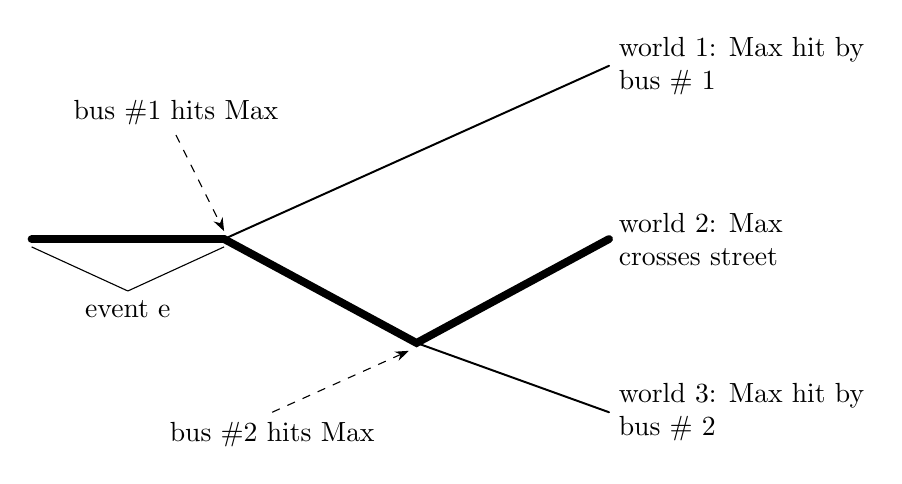
\begin{tikzpicture}
      \tikzmath{
        % x positions
        \x1 = 11;
        \xb1 = 2/9*\x1; \xb2 = 4/9*\x1; \xb3 = 6/9*\x1;
        % y positions
        \y1 = 2/5*\x1; \ymid = 1/2*\y1;
        \yw1 = \y1; \yw2 = 1/2*\y1; \yw3 = 0*\y1; \yb2 = 1/5*\y1;
        % event e
        \xe = 1/2*\xb1; \yediff = \yw2 - \yb2;
        \ye = \yw2 - 1/2*\yediff;
        \enudge = .1;
        \xel = 0; \xer = \xb1; \yen = \yw2 - \enudge;
        % bus 1 description location
        \xbx = 1.5/9*\x1; \xby = 4/5*\y1;
        % bus 2 description location
        \xb9 = 2.5/9*\x1;
      }
      % Paths
      \draw[line width=0.25mm, line cap=round] (\xb1,\ymid) -- (\xb3,\yw1); % world 1
      \draw[line width=1mm, line cap=round] (0,\ymid) -- (\xb1,\ymid) -- (\xb2,\yb2) -- (\xb3,\yw2); % world 2
      \draw[line width=0.25mm, line cap=round] (\xb2,\yb2) -- (\xb3,\yw3); % world 3
      % World descriptions
      \filldraw[black] (\xb3,\yw1) circle (0pt) node[anchor=west, align=left]{world 1: Max hit by \\ bus \# 1};
      \filldraw[black] (\xb3,\yw2) circle (0pt) node[anchor=west, align=left]{world 2: Max \\ crosses street};
      \filldraw[black] (\xb3,\yw3) circle (0pt) node[anchor=west, align=left]{world 3: Max hit by \\ bus \# 2};
      % Event
      \draw[] (\xe,\ye) -- (\xel,\yen); % event l
      \draw[] (\xe,\ye) -- (\xer,\yen); % event r
      % Event description
      \filldraw[black] (\xe,\ye) circle (0pt) node[anchor=north, align=left]{event e};
      % Splits
      \filldraw[black, dashed] (\xbx,\xby) circle (0pt) node[anchor=south, align=left]{bus \#1 hits Max};
      \filldraw[black, dashed] (\xb9,\yw3) circle (0pt) node[anchor=north, align=left]{bus \#2 hits Max};
      % Split descriptions
      \draw[-Stealth, dashed] (\xbx,\xby) -- (\xb1,\ymid + \enudge); % bus 2 arrow
      \draw[-Stealth, dashed] (\xb9,\yw3) -- (\xb2 - \enudge,\yb2 - \enudge); % bus 2 arrow
    \end{tikzpicture}
    \caption{
      Continuation path of `Max was crossing the street'. \\
    }
    \label{fig:max-bus}
  \end{figure}
\end{note}

% \begin{note}
% {
%   \color{red}
%   It's not obvious that this is the case on \citeauthor{Landman:1992wh}'s account.
% }
%   Max was rather unfortunate to be hit by a bus, but fortunes may be reversed.
%   The same reasoning applies to

%   \begin{enumerate}
%   \item
%     \label{prog:max:good}
%     Max was failing at the exam.
%   \end{enumerate}

%   Multiple choice.
%   Max goes for broke.
%   For each question, Max puts down the right answer.
%   However, Max was not destined to write down the correct answer there is a branch from how things actually happened in which Max chose the incorrect answer.
%   And, after a sequence of incorrect choices, Max failed the exam.
% \end{note}

\paragraph[\citeauthor{Landman:1992wh}~(\citeyear{Landman:1992wh})]{\citeauthor{Landman:1992wh}'s (\citeyear{Landman:1992wh}) account of the progressive}

\begin{note}
  \citeauthor{Landman:1992wh}'s account of the progressive:

  \begin{quote}
    \(\sem{\text{PROG}(e, P)}_{w,g} = 1\) iff \(\exists f \exists v\colon \langle f,v \rangle \in \text{CON}(g(e), w)\)\newline
    \phantom{an} and \(\sem{P}_{v,g}(f) = 1\)\par

    where \(\text{CON}(g(e), w)\) is the continuation branch of \(g(e)\) in \(w\).\newline
    \mbox{ }\hfill\mbox{(\citeyear[27]{Landman:1992wh})}
  \end{quote}

  Immediate goal is to present \citeauthor{Landman:1992wh}'s account of a continuation branch.
  In turn, this will require expansion on three further points.
  Stages of an event.
  Continuations and stops with respect to events.
  Reasonable options.

  With understanding in hand algorithmic reconstruction of continuation branch.
  Expand in two ways.
  First, tree, to allow for forks.
  Second, a different account of how to identify branches.
\end{note}

\subparagraph{Continuation branch}

\begin{note}
  \citeauthor{Landman:1992wh}'s account of a continuation branch is as follows:
  \begin{quote}
    The \emph{continuation branch} for \(e\) in \(w\) is the smallest set of pairs of events and worlds such that
    \begin{enumerate}
    \item
      \label{Landman:CB:continues}
      for every event \(f\) in \(w\) such that \(e\) is a stage of \(\langle f,w \rangle \in C(e,w)\);
      the continuation stretch of \(e\) in \(w\);
    \item
      \label{Landman:CB:stops}
      if the continuation stretch of \(e\) in \(w\) stops in \(w\), it has a maximal element \(f\) and \(f\) stops in \(w\).
      Consider the closest world \(v\) where \(f\) does not stop:
      \begin{enumerate}[label=--]
      \item
        if \(v\) is not in \(R(e, w)\), the continuation branch stops.
      \item
        if \(v\) is in \(R(e, w)\), then \(\langle f,v \rangle \in C(e,w)\).
        In this case, we repeat the construction:
      \end{enumerate}
    \item
      \label{Landman:CB:continues:again}
      for every \(g\) in \(v\) such that \(f\) is a stage of \(g\), \(\langle g,v \rangle \in C(e,w)\), the continuation stretch of \(e\) in \(v\);
    \item
      \label{Landman:CB:stops:again}
      if the continuation stretch of \(e\) in \(v\) stops, we look at the closest world \(z\) where its maximal element \(g\) does not stop:
      \begin{enumerate}[label=--]
      \item
        if \(z\) is not in \(R(e, w)\), the continuation branch stops.
      \item
        if \(z\) is in \(R(e, w)\), then \(\langle g,z \rangle \in C(e,w)\) and we continue as above, etc.%
        \mbox{ }\hfill\mbox{(\citeyear[26--27]{Landman:1992wh})}
      \end{enumerate}
    \end{enumerate}
  \end{quote}

  Describes the process of following an event \(e\) and a world \(w\) and jumping to nearby reasonable worlds when \(e\) stops in \(w\) (or \(w'\), etc.).

  Observe, the construction of a continuation branch is iterative.
  Clauses~\ref{Landman:CB:continues:again} and~\ref{Landman:CB:stops:again} and duplicates of Clauses~\ref{Landman:CB:continues} and~\ref{Landman:CB:stops} shifted to \(g\) --- some development of \(e\) --- in some possible world \(v\).

  Reconstruction via a recursive algorithm.
  For the moment we leave \citeauthor{Landman:1992wh}'s account of a continuation branch without commentary.
\end{note}

\subparagraph{Stages}

\begin{note}
  An event being a stage of some other event.
  Clause~\ref{Landman:CB:continues} (and~\ref{Landman:CB:continues:again}).

  \citeauthor{Landman:1992wh}'s definition is light:
  \begin{quote}
    An event is a stage of another event if the second can be regarded as a more developed version of the first, that is, if we can point at it and say, ``It's the same event in a further stage of development.''\newline
    \mbox{ }\hfill\mbox{(\citeyear[23]{Landman:1992wh})}
  \end{quote}
  \citeauthor{Landman:1992wh}'s definition is from an agent's perspective.
  Even if the elaboration is ignored, the initial expansion is qualified by the term `can be regarded as'.
  However, we may provide a definition of a stage independent of an agent's perspective:
  \begin{definition}[Stage]
    For events \(e\) and \(f\):

    \begin{itemize*}
    \item
      \(e\) is a stage of \(f\).
    \item
      \emph{If and only if}
    \item
      \(f\) is a development of \(e\).
    \item
      \mbox{ }
    \end{itemize*}
  \end{definition}
  At issue is what it is for \(f\) to be a \emph{development} of \(e\).

  Stage is distinguished from part-of.
  \nocite{Davidson:1967aa}

  Buttering the toast.
  Bread was toasted.
  But, toasting the bread was not a stage of buttering the toast.
  Sufficiently distinct events.
  Marked by `toast'.
  Toasting and buttering the bread, then plausible stage.
  Likewise, scooping butter onto the knife, stage of buttering the toast.

  Stage does not entail anything of significance happens.
  Waiting for the post to arrive.
  Stage, nothing is happening, event has developed.

  So, definition by intuitive distinction.

  Importance is for shifting-to and tracing-events-through possible worlds.
\end{note}

\subparagraph{Continuations and Stops}

\begin{note}[Continuations and Stops]
  The definition of a stage is important for defining both the continuation and when an event stops.
  We present \citeauthor{Landman:1992wh}'s definition of both terms, and then provide restated definitions.
\end{note}

\begin{note}
  \citeauthor{Landman:1992wh} combines the definition of a continuation and when an event stops:
  \begin{quote}
    This is where stages come in: we cannot say that when an event stops in a world, there is no bigger event of which it is part in that world, but we can say that when it stops, there is no bigger event in the world of which it is a \emph{stage}:
    \begin{enumerate}[label=, noitemsep]
    \item
      Let \(e\) be an event that goes on at \(i\) in \(w\).
      Let \(f\) be an event that goes on at \(j\) in where \(i\) is a subinterval of \(j\).
    \item
      \(j\) is a continuation of \(e\) iff \(e\) is a stage of \(f\).
    \item
      Let \(j\) be a non-final interval.
    \item
      \(f\) stops at \(j\) in \(w\) iff no event of which \(f\) is a stage goes on beyond \(i\) in \(w\) (i.e., at a later ending interval).\newline
      \mbox{ }\hfill\mbox{(\citeyear[23--24]{Landman:1992wh})}
    \end{enumerate}
  \end{quote}

  To clarify the definitions, we borrow the relevant definitions regarding intervals from \textcite{Dowty:1979vq}:

  \begin{quote}
    \(I\) is a subinterval of \(J\) iff \(I \subseteq J\), where \(I\) and \(J\) are intervals.
    \(I\) is a proper subinterval of \(J\) iff \(I \subset J\).
    \(I\) is an \emph{initial subinterval} of \(J\) iff \(I\) is a subinterval of \(J\) and there is no \(t \in (J - I)\) for which there is \(t' \in I\) such that \(t \leq t'\).
    \emph{Final subinterval} is defined similarly\dots\newline
    \mbox{ }\hfill\mbox{(\citeyear[140]{Dowty:1979vq})}
  \end{quote}
  So, following \citeauthor{Dowty:1979vq}:
  \begin{quote}
    \(I\) is a \emph{final subinterval} of \(J\) iff \(I\) is a subinterval of \(J\) and there is no \(t \in (J - I)\) for which there is \(t' \in I\) such that \(t' \leq t\).
  \end{quote}
  And, from the definition of a non-final subinterval follows similarly:
  \begin{quote}
    \(I\) is a \emph{non-final subinterval} of \(J\) iff \(I\) is a subinterval of \(J\) and there is \emph{some} \(t \in (J - I)\) for which there is \(t' \in I\) such that \(t' \leq t\).
  \end{quote}
  Intuitively, then, \(I\) is a \emph{non}-final interval of \(J\), just in case \(I \subseteq J\) and \(J\) progresses further in time than \(I\).

  Let us now turn to restating the definitions of a continuation and a stop.
  We take each in turn.
\end{note}

\begin{note}
  The definition of \(f\) being a continuation of \(e\) requires two things:
  First, it must be the case the event at which \(e\) takes place is a subinterval of the event at which \(f\) takes place, and it must be the case that \(e\) is a stage of \(f\).%
  \footnote{
    Though, it seems to me the latter/\ref{def:Landman:conts:stage} implies the former/\ref{def:Landman:conts:interval}.
    I.e.\ if \(e\) is a stage of \(f\) then the interval at which \(e\) takes place must be a subinterval of the interval at which \(f\) takes place.
  }
  In full:

  \begin{definition}[Continuations]
    \label{def:Landman:conts}
    For events \(e\) and \(f\):
    \begin{itemize}
    \item \(f\) is a \emph{continuation} of \(e\)
    \end{itemize}
    \emph{if and only if}
    \begin{itemize}
    \item
      The following jointly hold:
      \begin{enumerate}[label=\alph*., ref=(\alph*)]
      \item
        \label{def:Landman:conts:interval}
        \begin{enumerate}
        \item[\emph{If}:]
          \begin{enumerate}[label=\roman*.]
          \item
            \(i\) is the interval at which \(e\) takes place in \(w\).
          \end{enumerate}
        \item[\emph{And}:]
          \begin{enumerate}[label=\roman*., resume]
          \item
            \(j\) is the interval at which \(f\) takes place.
          \end{enumerate}
        \item[\emph{Then}:]
          \begin{enumerate}[label=\roman*., resume]
          \item
            \(i\) is a subinterval of \(j\).
          \end{enumerate}
        \end{enumerate}
      \item
        \label{def:Landman:conts:stage}
        \(e\) is a stage of \(f\).
      \end{enumerate}
    \end{itemize}
    \vspace{-\baselineskip}
  \end{definition}
\end{note}

\begin{note}
  The definition of \(f\) stopping at \(j\) in \(w\) takes a little more work.

  There are two immediate issues with \citeauthor{Landman:1992wh}'s definition.

  First, the definition requires that \(j\) is a non-final interval.
  But, of what?
  By assumption \(i\) is a subinterval of \(j\), so \(j\) cannot be a non-final interval of \(i\).%
  \footnote{
    The term `non-final interval' only appears in the above quote from \citeauthor{Landman:1992wh}.
  }

  Second, there must be no event of which \(f\) is a stage that goes beyond \(i\) in \(w\).
  However, by assumption \(f\) is an event that goes on at \(j\), and \(i\) is a subinterval of \(j\).
  But why is \(f\) bound by some arbitrary interval \(i\)?

  I propose to resolve both issues with the following definition:
  \begin{definition}[Stops]
    \label{def:Landman:Stops}
    For an event \(e\), interval \(i\), and world \(w\):
    \begin{itemize}
    \item
      \(e\) \emph{stops} at \(i\) in \(w\)
    \end{itemize}
    \emph{If and only if:}
    \begin{itemize}
    \item
      There no is interval \(j\) nor event \(f\) such that the following jointly hold:
      \begin{enumerate}[label=\alph*., noitemsep]
      \item
        \(i\) is non-final subinterval of \(j\).
      \item
        \(f\) goes on at \(j\).
      \item
        \(f\) is a stage of \(e\).
      \end{enumerate}
    \end{itemize}
    \vspace{-\baselineskip}
  \end{definition}
  In short, there is no expansion from \(i\) \emph{forward} in time to obtain an interval \(j\) such that an event which is a stage of \(e\) got on at \(j\).

  Hence, \autoref{def:Landman:Stops} captures \citeauthor{Landman:1992wh}'s initial gloss: `[W]hen [\(e\)] stops, there is no bigger event in the world of which [\(e\)] is a \emph{stage}' (\citeyear[23]{Landman:1992wh})
\end{note}

\begin{note}[Example of \autoref{def:Landman:Stops}]
  Interesting case to consider.
  Time limits.
  Running the race in record time.
  But, falls short of the record.

  Now, it may be false.
  Or, it may be true.
  Stops, no longer possible to complete race in record time.
  Shift to possible world.
  However, stops when event is still in progress.
  So, shift two possible world at time when stop will be completing race in record time.
\end{note}

\subparagraph{Reasonable options}

\begin{note}
  Reasonable options
  \begin{quote}
    \(v \in R(e, w)\) iff there is a reasonable chance on the basis of what is internal to \(e\) in \(e\) that \(e\) continues in \(w\) as far as it does in \(v\).%
    \mbox{ }\hfill\mbox{(\citeyear[26]{Landman:1992wh})}
  \end{quote}

  Look at possible worlds.
  Consider event \(e\) in possible world \(v\).
  Consider \(e\) in actual world.
  If there is a reasonable chance that \(e\) continues in \(w\) as in \(v\), then \(v\) is reasonable, on the basis of what is `internal' to \(e\).

  Not at all clear.
  However, significant insight from role in \citeauthor{Landman:1992wh}'s account of the progressive.
  \autoref{cha:sec:fcs-def:progressive-landman:alg:branches} considers in detail.

  Briefly, however, `reasonable' is intuitively epistemic, but need not be.
\end{note}

\paragraph{An algorithmic (re)construction}
\label{cha:sec:fcs-def:progressive-landman:alg}

\begin{note}
  Breaking this down into a recursive algorithm.
  Goal is to create a tree, which will be a set of ordered event-world-pairing pairs indexed according to depth.
  For example:
  \[\text{Tree} = \{\langle \langle e,w \rangle_{1}, \langle f,w \rangle_{1} \rangle, \langle \langle f,w \rangle_{1}, \langle g,v \rangle_{2} \rangle, \langle \langle f,w \rangle_{1}, \langle g,v' \rangle_{2} \rangle, \dots \}\]

  Root, inital event world pair, and then branch from event world pair to some distinct event world pair just in case ordered pair.
  %
  \footnote{
    The indexing is not required to construct the tree.
    However, important for keeping track of the stage of construction.
  }

  {\color{red} Pseudocode}
  \nocite{Cormen:2009uw}

  We start by identifying three basic functions, and following a (re)construction of these functions with explanation added, we (re)construct a recursive function to build a continuation branch of some event-world pairing.

  The four basic algorithms will be termed:
  `\AlgAC{}', `\AlgGetStops{}', `\AlgGetPStops{}', and `\AlgFindBranches{}'.
  The recursive algorithm will be termed:
  `\AlgDevelopTree{}'.

  Interest will be in difference between \AlgGetStops{} and \AlgGetPStops{}.
\end{note}

\subparagraph{Continuations}
\label{cha:sec:fcs-def:progressive-landman:alg:conts}

\begin{note}[\AlgAC{}]
  Clause~\ref{Landman:CB:continues} (and~\ref{Landman:CB:continues:again}) of \citeauthor{Landman:1992wh}'s definition of a continuation branch, which characterises the idea of a `continuation stretch' of some event \(g\) in world \(u\).
  We term the algorithm `\AlgAC{}':

  \begin{algorithm}[H]
    \label{PrAl:g-a-c}
    \caption{\AlgAC{}}
    \SetAlgoLined
    \DontPrintSemicolon
    \Input{\(\langle g,u \rangle_{i}\) \hfill An (indexed) event-world pairing}
    \KwResult{Continuation \hfill The continuation of \(g\) in \(u\)}
    \Begin{
      \(\text{Continuation} \longleftarrow \emptyset\)\;
      \label{PrAl:g-a-c:CSetInt}
      \(t_{s} \longleftarrow \text{start time of }g\text{ in }u\)\;
      \label{PrAl:g-a-c:ts}
      \(t_{e} \longleftarrow \text{end time of }g\text{ in }u\)\;
      \label{PrAl:g-a-c:te}
      \(g_{x} \longleftarrow g\)\;
      \label{PrAl:g-a-c:gx}
      \While{\(g_{x}\) is an event in \(u\)}
      {
        \label{PrAl:g-a-c:while:s}
        \(g_{x} \longleftarrow \emptyset\)\;
        \label{PrAl:g-a-c:gx:discard}
        \(t_{e} \longleftarrow t_{e} + 1\)\;
        \label{PrAl:g-a-c:te:plus}
        \(I \longleftarrow [t_{s},t_{e}]\)\;
        \label{PrAl:g-a-c:te:I}
        \For{\(g_{y} \in \{g_{y} \mid g_{y} \text{ is an event in } u\}\)}{
          \label{PrAl:g-a-c:for:s}
          \If{\(g_{y}\) occurs in \(I\) \emph{and} \(g_{y}\) is a stage of \(g\)}
          {
            \label{PrAl:g-a-c:for:test}
            \(\text{Continuation} \longleftarrow \text{Continuation} \cup \langle \langle g_{x},u \rangle_{i}, \langle g_{y},u \rangle_{i} \rangle\)\;
            \label{PrAl:g-a-c:C:new}
            \(g_{x} \longleftarrow g_{y}\)\;
            \label{PrAl:g-a-c:gx:new}
          }
        }
      }
      \label{PrAl:g-a-c:while:e}
      \Return{\(\text{Continuation}\)}
      \label{PrAl:g-a-c:return}
    }
  \end{algorithm}

  \AlgAC{} takes an event-world pairing \(\langle g,u \rangle_{i}\) and returns a set containing a (non-branching tree) which captures the continuation stretch of \(g\) in \(u\).

  Intuitively, \AlgAC{} starts with \(\langle g,u \rangle_{i}\).
  Then, \AlgAC{} finds the smallest event \(g^{+}\) such that \(g^{+}\) is a stage of \(g\) in \(u\), and adds \(\langle g,u \rangle_{i}, \langle g^{+},u \rangle_{i} \rangle\) as a continuation.
  Now, \(g\) may develop further in \(u\).
  So, \AlgAC{} continues to the smallest \(g^{++}\) such that \(g^{++}\) is a stage of \(g\) in \(u\) at a later time than \(g^{+}\), and adds \(\langle g^{+},u \rangle_{i}, \langle g^{++},u \rangle_{i} \rangle\) as a continuation.
  The hypothetical set \(\text{Continuation}\) is now \(\{\langle g,u \rangle_{i}, \langle g^{+},u \rangle_{i} \rangle, \langle g^{+},u \rangle_{i}, \langle g^{++},u \rangle_{i} \rangle\}\).

  This process repeats until there are no further stages of \(g\) in \(u\).
\end{note}

\begin{note}[Motivation for \AlgAC{}]
  There are two pieces of motivation for the construction of \(\text{Continuation}\).

  The first piece of motivation is \citeauthor{Landman:1992wh}'s account of the progressive.
  For, \(\sem{\text{PROG}(e, P)}_{w,g}\) checks to see if there exists \emph{some} event-world pairing \(\langle f,v \rangle\) in the continuation branch of \(e\) (in \(w\)) such that \(\sem{P}\) is true of \(f\) in \(v\).
  Hence, it is not possible, in general, to only consider the `maximal' continuation of \(g\) in \(u\).
  Rather, we must have the option of identifying the particular stage \(f'\) of \(f\) such that \(P\) is true of \(f'\).

  The second piece of motivation is the critiques of \textcite{Bonomi:1997uq} and \textcite{Szabo:2004ul} which suggest modifying \citeauthor{Landman:1992wh}'s account of the progressive to include universal quantification over branches of a continuation tree.
  Therefore, it is important to ensure that the continuation of \(g\) in \(u\) does not itself involve branching.%
  \footnote{
    I.e., this constraint rules out including both \(\langle \langle g,u \rangle_{i}, \langle g^{+},u \rangle_{i} \rangle\) and \(\langle \langle g,u \rangle_{i}, \langle g^{++},u \rangle_{i} \rangle\), as this would indicate a branch.
  }
\end{note}

\begin{note}[Construction of \AlgAC{}]
  Finally, then, we have the way in which \(\text{Continuation}\) is constructed.

  We start by initialising \(\text{Continuation}\) as an empty set (\autoref{PrAl:g-a-c:CSetInt}).
  Then, we identify the start and end times of the interval in which \(g\) takes place (Lines~\ref{PrAl:g-a-c:ts} and~\ref{PrAl:g-a-c:te}).

  The task is then to continue to expand \(\text{Continuation}\) so long as there are further stages of \(g\) in \(u\).
  We achieve this a while loop %
  (Lines~\ref{PrAl:g-a-c:while:s}--\ref{PrAl:g-a-c:while:e}) %
  that will fail when we are no longer considering an event in \(u\).
  The variable event \(g_{x}\) is initially set to \(g\), to guaranteed at least one pass through the loop (\autoref{PrAl:g-a-c:gx}).

  In a instance of the while loop we first discard \(g_{x}\) to ensure the loop will fail if there are no further stages of \(g\) (\autoref{PrAl:g-a-c:gx:discard}).
  Then, we construct an interval \(I\) by shifting forward one step in time (Lines~\ref{PrAl:g-a-c:te:plus}~and~\ref{PrAl:g-a-c:te:I}).

  At this point, we have a new interval \(I\) to consider, but no immediate event.
  So, we consider every event \(g_{y}\) which occurs in \(u\) and test to see if \(g_{y}\) happens in \(I\) \emph{and} is a stage of \(g\) (Lines~\ref{PrAl:g-a-c:for:s}~and~\ref{PrAl:g-a-c:for:test}).
  If successful, we update \(\text{Continuation}\) and \(g_{x}\) (Lines~\ref{PrAl:g-a-c:C:new}~and~\ref{PrAl:g-a-c:gx:new}).

  Here we make two assumptions:
  \begin{itemize}[noitemsep]
  \item
    First, if there is some stage of \(g\), then there is stage of \(g\) at an interval obtained by stepping one tick forward in time.%
  \footnote{
    This may be avoided by separating the test on~\autoref{PrAl:g-a-c:for:test} into two separate tests, and shifting the reassignment on~\autoref{PrAl:g-a-c:gx:new} outside the scope of the if-clause.
    Though the while-loop will then only terminate when there are no further events in \(u\).
  }
  \item
    Second, for any interval, if there is an event which is a stage of \(g\), then the event is unique.%
    \footnote{
      This assumption is key to ensure \(\text{Continuation}\) does not introduce branching.
      Though, the assumption may be avoided by choosing a different representation for the tree.
    }
  \end{itemize}

  After the stages of \(g\) in \(u\) have been exhausted, \AlgAC{} returns \(\text{Continuation}\) (\autoref{PrAl:g-a-c:return}) and terminates.
\end{note}

\subparagraph{Stops}
\label{cha:sec:fcs-def:progressive-landman:alg:stops}

\begin{note}[\AlgGetStops{}]
  To the \emph{antecedent} of Clause~\ref{Landman:CB:stops} (and~\ref{Landman:CB:stops:again}) of \citeauthor{Landman:1992wh}'s definition of a continuation branch asks whether the continuation stretch of \(g\) stops in \(u\), and considers the `maximal' event \(g'\) in \(u\) (if \(g\) stops).

  Intuitively, the algorithm `\AlgGetStops{}' searches through some continuation stretch of \(g\) in \(i\) (i.e.\ the result of \AlgAC{\((\langle g,u \rangle_{i})\)}) to identify the stopping point of \(g\) in \(u\).
  Hence, if \(g\) stops in \(u\) \AlgGetStops{} returns the relevant `maximal' event.
  Otherwise, \AlgGetStops{} does not return an event-world pairing.
  So, by inspecting the result of \AlgGetStops{} we may determine whether the antecedent of Clause~\ref{Landman:CB:stops} (and~\ref{Landman:CB:stops:again}) is fulfilled.

  Strictly, the construction of \AlgGetStops{} is generalised to cover finding the stopping points of multiple continuation stretches, but the same intuition extends to the more general case.

  After identifying the relevant stopping points of an event \(g\) in world \(u\), the following task will be to find continuations of \(g\) in other worlds.

  \AlgGetStops{} is as follows:

  \begin{algorithm}[H]
    \label{PrAl:g-s}
    \caption{\AlgGetStops{}}
    \SetAlgoLined
    \DontPrintSemicolon
    \Input{\(\text{Continuations}\) \hfill I.e.\ results of \AlgAC{} --- in general, a tree}
    \KwResult{Stops \hfill Stopping points for each event in \(\text{Continuations}\)}
    \Begin{
      \(\text{Stops} \longleftarrow \emptyset\)\;
      \label{PrAl:g-s:mk-st-Stops}
      \For{\(\langle \langle f,v \rangle_{i-1}, \langle g,u \rangle_{i} \rangle \in \text{Continuation}\)}
      {
        \label{PrAl:g-s:for:start}
        \If{\(g\text{ stops in }u\)}
        {
          \label{PrAl:g-s:if:start}
          % \(g' \longleftarrow\text{ the stopping point of }g\text{ in }u\)\;
          % \label{PrAl:g-s:max}
          \(\text{Stops} \longleftarrow \text{Stops} \cup \{\langle \langle f,v \rangle_{i-1}, \langle g,u \rangle_{i} \rangle\}\)\;
          \label{PrAl:g-s:make}
        }
      }
      \Return{\(\text{Stops}\)}
      \label{PrAl:g-s:return}
    }
  \end{algorithm}
\end{note}

\begin{note}[Construction of \AlgGetStops{}]
  The construction of \AlgGetStops{} is simple:%
  \footnote{
    \AlgGetStops{} differs in presentation from \citeauthor{Landman:1992wh}.
    Recall:
    \begin{quote}
      \begin{enumerate}
        \setcounter{enumi}{1}
      \item
        if the continuation stretch of \(e\) in \(w\) stops in \(w\), it has a maximal element \(f\) and \(f\) stops in \(w\).
        Consider the closest world \(v\) where \(f\) does not stop:\dots
      \end{enumerate}
    \end{quote}
    Clause~\ref{Landman:CB:continues} reads as an imperative to find the relevant maximal event.
    Still, so long as \AlgGetStops{} is applied to results \AlgAC{}, the result is equivalent, for the set of continuation given by \AlgAC{} will include the relevant maximal event.
  }

  \AlgGetStops{} initialises \(\text{Stops}\) as an empty set (\autoref{PrAl:g-s:mk-st-Stops}), and for every element of \(\text{Continuations}\), \AlgGetStops{} takes the right-event-world pairing and queries whether the event stops in the world (Lines~\ref{PrAl:g-s:for:start}--\ref{PrAl:g-s:if:start}).
  If the event stops, \AlgGetStops{} takes the point at which the event stops and adds the element of \(\text{Continuations}\)%
  % with the maximal continuation substituted for the event
  to \(\text{Stops}\) (\autoref{PrAl:g-s:make}).
  \AlgGetStops{} returns \(\text{Stops}\) (\autoref{PrAl:g-s:return}) and terminates.
\end{note}

\begin{note}
  Applied to a single instance of \AlgAC{}, \AlgGetStops{} will either return an empty set or a singleton set containing a pairing in which the event of the right element stops.
  And, applied to a set containing multiple results of \AlgAC{}, \AlgGetStops{} will either return an empty set or a set of size bounded by the instances of \AlgAC{}.
\end{note}

\begin{note}
  Role of \AlgGetStops{} is somewhat artificial.
  It would be far more effective to identify a stopping event in the construction of \AlgAC{}.

  However, after introducing \AlgFindBranches{} to find the continuations of a stopping event in some possible world (\autoref{cha:sec:fcs-def:progressive-landman:alg:branches}) we will introduce variant of \AlgGetStops{} (\autoref{cha:sec:fcs-def:progressive-landman:alg:R-stops}).
\end{note}

\subparagraph{Branches}
\label{cha:sec:fcs-def:progressive-landman:alg:branches}

\begin{note}
  The \emph{consequent} of Clause~\ref{Landman:CB:stops} (and~\ref{Landman:CB:stops:again}) of \citeauthor{Landman:1992wh}'s definition of a continuation branch requires identifying the continuation of an event \(g\) which stops in \(u\) in some possible world \(u'\), if the continuation exists.

  The algorithm `\AlgFindBranches{}' is designed to return such continuations of event-world pairings in general.%
  \footnote{
    As with \AlgGetStops{}, the existence of a continuation is given by contrasting the inputs to the output of \AlgFindBranches{}.
  For, if \(\langle \langle f,v \rangle_{i-1}, \langle g,u \rangle_{i}\rangle\) is an element of the input to \AlgGetStops{}, then there is a continuation of \(g\) in some other world \(u'\) just in case \(\langle \langle f,v \rangle_{i-1}, \langle g,u' \rangle_{i}\rangle\) is an element of the output.
  }
  Though, the primary use-case is applying \AlgFindBranches{} to the result of \AlgGetStops{}.

  \AlgFindBranches{} is as follows:

  \begin{algorithm}[H]
    \label{PrAl:find-branches}
    \caption{\AlgFindBranches{}}
    \SetAlgoLined
    \DontPrintSemicolon
    \Input{\(\langle \langle f,v \rangle_{i-1}, \langle g,u \rangle_{i}\rangle\) \hfill An element of a tree\\
      \(e\) \hfill An event \\
      \(w\) \hfill A world
    }
    \KwResult{Branches \hfill A set containing event-world pairs \\
      \hfill such that \(g\) continues in \(u'\)}
    \Begin{
      \(\text{CloseWorlds} \longleftarrow \{u' \mid u' \text{ is among the closest world to } u\}\)\;
      \label{PrAl:find-branches:close}
      \(\text{ReasonableWorlds} \longleftarrow \text{CloseWorlds} \cap R(e,w)\)\;
      \label{PrAl:find-branches:loop:R}
      \(\text{Branches} \longleftarrow \emptyset\)\;
      \For{\(u' \in \text{ReasonableWorlds}\)}{
        \label{PrAl:find-branches:loop:start}
        \If{\(g\) is an event in \(u'\)}{
          \(\text{Branches} \longleftarrow \text{Branches} \cup \{ \langle \langle f,v \rangle_{i-1}, \langle g,u' \rangle_{i}\rangle \}\)\;
        }
      }
      \label{PrAl:find-branches:loop:end}
      \Return{\(\text{Branches}\)}
    }
  \end{algorithm}
\end{note}

\begin{note}
  From a broad perspective, \AlgFindBranches{} considers some event-world pairing \(\langle g,u \rangle\) and returns a collection of event-world pairings \(\langle g,u' \rangle\) where \(u'\) is some possible world.

  From this broad perspective, the core of \AlgFindBranches{} is a for-loop (Lines~\ref{PrAl:find-branches:loop:start}--\ref{PrAl:find-branches:loop:end}) which scans through some collection of possible worlds and identifies those worlds in which \(g\) is present in the possible world.

  From a more nuanced perspective, the core of \AlgFindBranches{} is with how the possible worlds are specified (i.e.\ Lines~\ref{PrAl:find-branches:close} and~      \ref{PrAl:find-branches:loop:R}).
\end{note}

\begin{note}
  Let us begin by considering \AlgFindBranches{} applied to a particular event-world pair \(\langle g,u \rangle\).

  First, observe that \(g\) is an event in \(u\).
  Hence, \AlgFindBranches{} return some \(\langle g,u' \rangle\)-pairing such that \(g\) happened in \(u'\) in parallel to \(g\) happening in \(u'\).
  Stressed, \AlgFindBranches{} \emph{does not} return \(\langle g,u' \rangle\)-pairing such that \(g\) happened in \(u'\) even though \(g\) didn't happen in \(u'\).
  This follows \citeauthor{Landman:1992wh}'s definition.
  For, while \(g\) stopping in \(u\) means only that \(g\) does not continue in \(u\) (cf.~\autoref{def:Landman:Stops} on \autopageref{def:Landman:Stops}).

  In turn, this means \(\langle g,u' \rangle\) may be passed as an argument to \AlgFindBranches{}.
  So, second, observe Line~\autoref{PrAl:find-branches:close} considers possible worlds close to the argument event-world pairing.
  Hence, repeated application of \AlgFindBranches{} may lead to `drift'.
  \(u'\) may be close to \(u\), and \(u''\) may be close to \(u'\), but \(u''\) need not be close to \(u\).
  This is an important feature of \citeauthor{Landman:1992wh}'s account of the progressive.
  Recall the instance of the progressive from \autopageref{prog:max:bad}:
  \begin{enumerate}
  \item
    Max is crossing the street.
  \end{enumerate}
  Also recall \ref{prog:max:bad} is true even though Max is hit by a bus.
  Now, in close worlds to the actual world, Max may be hit by a bus in various different ways, and hence there is no close world \emph{to the actual world} in which Max crosses the street.
  However, by the process of drifting through possible worlds, we expect to find a possible world in which Max is not hit by a bus (and crosses the street).
  {
    \color{red} not to counterfactual reduction?
  }

  However, in principle it seems possible to drift though possible worlds so that (almost) any arbitrary eventuality results from some event.
  The point is especially clear if we combine \AlgFindBranches{} with \AlgAC{} to allow events to develop.

  Now, consider:
  \begin{enumerate}[label=\arabic*., ref=(\arabic*)]
    \setcounter{enumi}{1}
  \item
    Cyril is stating the first ten digits of (the decimal representation of) \(\pi\).
  \end{enumerate}
  Cyril does not know the first ten digits of \(\pi\) but has started with `\(3\)' and then `\(1\)'.
  In the actual world, Cyril it interrupted, but in a close world Cyril utters `\(4\)', and we may continue drifting through possible worlds until Cyril utters the first ten digits of \(\pi\).%
  \footnote{
    And, indeed any finite sequence of digits from (the decimal representation of) \(\pi\).
    See \citeauthor{Landman:1992wh} (\citeyear[\S2.3]{Landman:1992wh}) for additional examples and discussion.
  }

  Considerations such as the above motivate Line~\ref{PrAl:find-branches:loop:R}.
  Recall:
  \begin{quote}
    \(v \in R(e, w)\) iff there is a reasonable chance on the basis of what is internal to \(e\) in \(e\) that \(e\) continues in \(w\) as far as it does in \(v\).%
    \mbox{ }\hfill\mbox{(\citeyear[26]{Landman:1992wh})}
  \end{quote}
  Consider a possible world where \(e\) continues, and query whether \(e\) may have continued in \(v\).

  Phrased otherwise, \(\text{CloseWorlds}\) captures closeness between worlds, while \(R(e,w)\) captures closeness between events.

  Perhaps uttering `\(4\)' in place of `\(5\)' is reasonable, but as we progress through `\(1\)', `\(5\)', `\(9\)', `\(2\)', \dots it is, intuitively, quite unreasonable.
  For that Cyril does not know the first ten digits of \(\pi\).
  Hence, Cyril uttering the correct sequence of digits would require considerable luck.%
  \footnote{
    If ten digits seems borderline, extend the sequence.
    Given a decimal representation and random choice by Cyril, the probability of the Cyril uttering the correct sequence is \(.1^{l}\) where \(l\) is the length of the sequence.
  }
  In addition, note the set of reasonable worlds is determined by two arguments given to \AlgFindBranches{} that are independent of the event-world pairing given as an argument.
  Intuitively, and in practice, these arguments correspond to the initial event and world from which the continuation tree is constructed.
  Therefore, the extent to which \AlgFindBranches{} may lead to drift through possible worlds is limited by the initial event in the actual world.
\end{note}

\begin{note}
  Still, \citeauthor{Landman:1992wh}'s account is difficult.

  Unclear how to think about \(e\) continuing in \(w\).
  Can't be closest worlds in which \(e\) does not stop.
  For, by assumption, drifted from \(w\).

  Problem to solve is clear.
  Allow event to drift, but not indefinitely.
  And, restriction given by initial event in actual world.
  Events in progress.
  Failure not because there is no possibility, but because things required to secure possibility stray too far from the event as it has developed in the actual world.

  So, \(g\) is a reasonable stage of \(e\).

  Following \citeauthor{Landman:1992wh}, no way to reduce to similarity between worlds.
  For, \citeauthor{Landman:1992wh} holds that unreasonable even though what happened.
  Suppose Cyril hadn't been interrupted.
  Still unreasonable.

  Best I can do, if \(g\) then \(e\) from \(w\), where restrict interest in \(w\) up until \(e\) happening and interest in worlds up until \(g\) happens.%
  \footnote{
    \color{red}
    May captured by attention to fact.

  \citeauthor{Veltman:2005tj}'s (\citeyear{Veltman:2005tj}) revision to~\citeauthor{Tichy:1976tp}'s (\citeyear{Tichy:1976tp}) counterexample to \citeauthor{Lewis:1979vm}'s (\citeyear{Lewis:1973th,Lewis:1979vm}) theory of counterfactuals.

  Some `facts' are fixed, and it is not possible to alter these facts under a counterfactual assumption.
  \(e\) has been set in motion.
  Now, keeping \(e\) fixed, if not X then e would continue.

  Fix what has been set in motion by \(e\), keep all laws the same.
  Then, buses at different times, but Mary doesn't get superpowers.
  }
  So, getting \(g\) `because' continuation of \(e\).

  These are different.
  For, we look to see whether \(g\) is the case in \(u'\) but also that \(g\) is the result.
  Though, this clause is indirect.
  Really part of \AlgAC{}.
  Inefficient, but better placed here.
  As, we won't include in tree if not returned by this algorithm.
\end{note}

\begin{note}
  Motivated restriction on world.
  What about converse?
  Is it possible to consider only the `reasonable' worlds?
  No, because requires that search for \(g\).
  Even after drifting, don't get a continuation of \(g\) in close worlds.
\end{note}

\begin{note}
  See if the event at some world continues in some other world.
  \citeauthor{Landman:1992wh} assumes closest world, but following \textcite[37]{Szabo:2004ul} and~\textcite{Bonomi:1997uq}, allow for multiple close worlds.%
  \footnote{
    See in particular \citeauthor{Bonomi:1997uq}'s discussion of the `multiple-choice paradox' (\citeyear[\S4]{Bonomi:1997uq}).
  }
  Note, importance of \(e\) and \(w\)!
  No shift in index, as the function identifies the same event in some other possible world.
\end{note}

\begin{note}
  Two general notes:

  \citeauthor{Landman:1992wh}, existential, so risk of finding some continuation in `unreasonable' worlds.
  Now suggested universal, then failure in an `unreasonable' world does not entail failure of the progressive.
\end{note}

\begin{note}
  Here, shift the index.
  When run recursive algorithm, each call of the algorithm will explore branches.
  Increase index for next call.

  Also, note, \AlgGetPStops{}.
  Pass the result of \AlgGetPStops{}, and this will get 
\end{note}

\subparagraph{Reasonable stops}
\label{cha:sec:fcs-def:progressive-landman:alg:R-stops}

\begin{note}
  In \autoref{cha:sec:fcs-def:progressive-landman:alg:R-stops} we gave a reconstruction of the antecedent of Clause~\ref{Landman:CB:stops} (and~\ref{Landman:CB:stops:again}) of \citeauthor{Landman:1992wh}'s definition of a continuation branch.

  In this section, we motivate and detail an alternative algorithm.

  The basic observations are
  \begin{enumerate}[label=\arabic*., ref=(\arabic*), noitemsep]
  \item
    \label{landman:alg:R-stops:ob:1}
    If an agent performs some action \(\alpha\), then so long as \(\alpha\) is not instantaneous, there is some prior event such that the agent is \(\alpha\)ing.
  \item
    \label{landman:alg:R-stops:ob:2}
    It is not the case that Observation~\ref{landman:alg:R-stops:ob:1} holds, in general.
  \end{enumerate}
  To resolve this tension, we consider a modification of \AlgGetStops{} which returns `reasonable' rather than actual stops of an event.
  We term the modification `\AlgGetPStops{}'.

  First, we substantiate Observations~\ref{landman:alg:R-stops:ob:1} and~\ref{landman:alg:R-stops:ob:2}.
\end{note}

\begin{note}
  Observation~\ref{landman:alg:R-stops:ob:1} follows from  Clause~\ref{Landman:CB:stops} (and~\ref{Landman:CB:stops:again}) of \citeauthor{Landman:1992wh}'s definition of a continuation branch.
  For, Clause~\ref{Landman:CB:stops} (and~\ref{Landman:CB:stops:again}) is a conditional:
  \begin{quote}
    \begin{enumerate}
      \setcounter{enumi}{1}
    \item
      if the continuation stretch of \(e\) in \(w\) stops in \(w\), it has a maximal element \(f\) and \(f\) stops in \(w\).
      Consider the closest world \(v\) where \(f\) does not stop: \dots
    \end{enumerate}
  \end{quote}
  Hence, for an event \(e\) and world \(w\), Clause~\ref{Landman:CB:stops} only includes the closest world where \(e\) does not stop \emph{if} \(e\) stops in \(w\).
  So, if \(e\) does not stop in the actual world, and \(e\) develops into an event \(e'\) such that the agent \(\alpha\)s in \(e'\), then it will be true that the agent is \(\alpha\)ing with respect to \(e\).
\end{note}

\begin{note}
  We now turn to Observation~\ref{landman:alg:R-stops:ob:2}.

  Observation~\ref{landman:alg:R-stops:ob:2} is the converse of the above%
  \footnote{
    See the discussion of the imperfective paradox on~\autopageref{imperfective-paradox:intro}.
  }
  observation that an event in which an agent \(\alpha\)s does not need to happen for it to be true that the agent is \(\alpha\)ing.
  For, restated, Observation~\ref{landman:alg:R-stops:ob:2} reads:%
  \footnote{
    \citeauthor{Landman:1992wh} considers a similar observation under the term `the problem of non-interruptions' (\citeyear[14--17,30--31]{Landman:1992wh}).
    \citeauthor{Landman:1992wh}'s suggestion is to distinguish events by the perspective of the agent. (\citeyear[31]{Landman:1992wh})
    The basic idea, as I understand \citeauthor{Landman:1992wh} is to deny that the event \(e'\) in which the agent \(\alpha\)s is sufficiently distinct from any prior event \(e\).
    Hence, it seems that strictly speaking \citeauthor{Landman:1992wh} does not endorse Observation~\ref{landman:alg:R-stops:ob:2}.
  }
  \begin{enumerate}[label=\arabic*\('\)., ref=(\arabic*\('\))]
    \setcounter{enumi}{1}
  \item
    There are cases in which \(e\) is not an instance of an agent \(\alpha\)ing, though \(e\) develops into \(e'\) and \(e'\) is an event in which the agent \(\alpha\)s.
  \end{enumerate}

    We present a pair of \illu{1} with both provide instances of Observation~\ref{landman:alg:R-stops:ob:2}.
    Following, we turn to theoretical motivation.
\end{note}

\begin{note}
  \begin{illustration}[Flipping coins]
    \label{illu:fc:coins}
    Agent is flipping a coin in the air and recording how it lands.%
    \footnote{
      Cf.~\textcite{Gelman:2002ww} and~\textcite{Keller:1986tz}.
    }
    The coin lands heads ten times in a row.

    The following seem true:
    \begin{itemize}
    \item
      The coin landed heads ten in a row.
    \item
      The agent landed the coin heads ten times in a row.
    \end{itemize}
    However, the following seem false:
    \begin{itemize}
    \item
      The coin was landing heads ten times in a row.
    \item
      The agent was landing a coin heads ten times in a row.
    \end{itemize}
    \vspace{-\baselineskip}
  \end{illustration}
  Intuition is clear.
  No time prior to the coin landing heads on the tenth flip was the coin landing heads ten times in a row.
  Consider prior.
  \begin{itemize}
  \item
    I am landing this coin heads ten times in a row.
  \end{itemize}
  Only reasonable interpretation is if the agent will continue to keep flipping the coin until the coin lands heads ten times in a row.
  However, if the agent is limited to ten flips, absurd.

  Though, the tenth flip is a clear continuation of the event containing the previous nine coin flips.

  Possible objection.
  Event was not the result of the agent.
  And, if agent then works out because prior to agent completing action, progressive.
  However, the action is flipping the coin so that it lands heads.
  No different from encrypting a message so that it will not be understood by the messenger.
  Once sent, the agent has no involvement in the messenger's understanding.
  Though, given a sufficiently strong algorithm, it seems true that the agent is encrypting the message when working through the algorithm.
\end{note}

\begin{note}[Second]
  \begin{illustration}[Chess III]
    \label{illu:fc:chess:III}
    Consider as the game state on the left transitions to the game state on the right.

    \noindent\mbox{ }\hspace{2em}%
    \begin{adjustbox}{minipage=.4\linewidth,scale=.75}%
      \centering%
      \newchessgame[%
      setwhite={ka6,pa5,pb6,pc7,rg2,bh1},%
      addblack={ka8,rg8,na3},%
      ]%
      \setchessboard{showmover=false}%
      \chessboard%
    \end{adjustbox}%
    \hfil%
    \begin{adjustbox}{minipage=.4\linewidth,scale=.75}%
      \centering%
      \newchessgame[%
      setwhite={ka6,pa5,pb6,pc7,rg2,bh1},%
      addblack={ka8,rc8,na3},%
      ]%
      \setchessboard{showmover=false}%
      \chessboard%
    \end{adjustbox}%
    \hspace{2em}\mbox{ }

    On the left, white has just moved their pawn from c6 to c7.
    Though, white is quite bad at chess.
    And, the strength of their pieces on the board is the result of black intentionally playing even worse.
    So, it is not true that:
    \begin{itemize}
    \item
      White is winning the game of chess.
    \end{itemize}
    For example, if black moves their rook to h8 then on the following turn white may move their pawn to c8 and exchange it for a rook which black may then capture, etc.\dots

    Still, on the following turn, black moves their rook from g8 to c8, as shown on the right.
    As a result:
    \begin{itemize}
    \item
      White wins the game of chess.
    \end{itemize}
  \end{illustration}

  May argue about the interpretations of `wins'.
  For, white still needs to make a move.
  However, any move made by white results in checkmate for black.
  Hence, true.

  In contrast to \autoref{illu:fc:coins}, \autoref{illu:fc:chess:III} does not involve luck.
  Instead, \autoref{illu:fc:chess:III} involves the action by some other agent which leads to desired outcome.
  %
  \footnote{
    More generally, one consider the structure of \autoref{illu:fc:chess:III} applied to any competitive activity in which a mistake by one participant hands victory to the other participant.
    It seems clear to me that a win does not entail that the participant was winning at any point throughout the game.
    E.g.\ a racing car driver may be handed a win due to their competitor having a bad pit stop, or a football team may be handed a win due to an unexpected injury on the other team, etc.
  }
\end{note}

\begin{note}[Theoretical motivation]
  On the one hand, intuition.
  On the other hand, motivated by \citeauthor{Landman:1992wh}'s analysis.
  Distinction between event and world.
  Interested in the event getting to completion regardless of what happens in the world.
  Hence, allows us to shift to possible worlds.
  Progressive is not false because of contingencies of the actual world.
  By parallel, progressive is not true because of contingencies of actual world.
\end{note}

\begin{note}
  Given this, understand both \illu{1}.
  Deviance.

  Once noted, plausible to distinguish where in event progressive comes true.
  Final \illu{}.
  \begin{illustration}[Choosing cards]
    An agent is presented with a shuffled deck of playing cards and is asked to choose a number \(1 < n \leq 52\).
    After the agent announces the number, the presenter of the deck of cards will remove \(n - 1\) cards from the top of the deck and reveal the \(n\)th card.

    The agent considers their options with gravitas.
    \begin{itemize}
    \item
      First, the agent decides they will choose and odd number
    \item
      Second, the agent decides they will choose a card from the top half of the deck.
    \item
      Third, the agent decides they will choose a prime number.
    \item
      Finally, the agent chooses \(17\).
    \end{itemize}
    The agent is unaware that the pack is shuffled so that every card corresponding to a prime number is a red card, though the \(9\)th card isn't a red card.
    Hence, after the third choice, but not before, it is true that:
    \begin{itemize}
    \item
      The agent is choosing a red card.
    \end{itemize}
    \vspace{-\baselineskip}
  \end{illustration}
  So, before third decision, agent may have chosen a non-prime number.
  In particular, \(9\) is not a prime number and the \(9\)th card is not a red card.
  However, after the decision, no turning back.
\end{note}

\begin{note}
  So, Observations~\ref{landman:alg:R-stops:ob:1} and~\ref{landman:alg:R-stops:ob:2}.

  The suggestion is simple.
  Rather than search the continuation of an event \(f\) in world \(v\) 

  Slight difficulty is closest world.
  Instead, closest worlds.
  Intuitively, obtained from counterfactuals against what happened in the actual world.
  However, reasonable, as these are worlds in which the event continues.
\end{note}

\begin{note}
  Modification builds on principles for \AlgFindBranches{}.
  For, \AlgFindBranches{} finds continuation of event in nearby world.


  \AlgGetPStops{}:

  \begin{algorithm}[H]
    \label{PrAl:g-s}
    \caption{\AlgGetPStops{}}
    \SetAlgoLined
    \DontPrintSemicolon
    \Input{%
      \(\text{Continuation}\) \hfill I.e.\ the result of \AlgAC{} --- in general, a tree \\
      \(e\) \hfill An event \\
      \(w\) \hfill A world
    }
    \KwResult{ReasonableStops \hfill \emph{Reasonable} stopping points \\
      \mbox{ } \hfill for each event in \(\text{Continuation}\)}
    \Begin{
      \(\text{R-Stops} \longleftarrow \emptyset\)\;
      \For{\(\langle \langle f,v \rangle_{i-1}, \langle g,u \rangle_{i} \rangle \in \text{Continuation}\)}
      {
        \(\text{Branches} \longleftarrow \AlgFindBranches{(\langle \langle f,v \rangle_{i-1}, \langle g,u \rangle_{i} \rangle, e,w)}\)\;
        \For{\(\langle \langle f,v \rangle_{i-1}, \langle g,u' \rangle_{i} \rangle \in \text{Branches}\)}
        {
          \If{\(g\text{ stops in }u'\)}
          {
            \(\text{R-Stops} \longleftarrow \text{R-Stops} \cup \{\langle \langle f,v \rangle_{i-1}, \langle g,u' \rangle_{i} \rangle\}\)\;
          }
        }
      }
      \Return{\(\text{R-Stops}\)}
    }
  \end{algorithm}

  Test%
  \footnote{
    Expanding and simplifying a little, the body of \AlgGetPStops{} reads:

    \begin{algorithm}[H]
      % \SetAlgoLined
      \DontPrintSemicolon
      \Begin{
        \(\text{R-Stops} \longleftarrow \emptyset\)\;
        \For{\(\langle \langle f,v \rangle_{i-1}, \langle g,u \rangle_{i} \rangle \in \text{Continuation}\)}
        {
          \(\text{CloseWorlds} \longleftarrow \{u' \mid u' \text{ is among the close world to } u\}\)\;
          \(\text{ReasonableWorlds} \longleftarrow \text{CloseWorlds} \cap R(e,w)\)\;
          \For{\(u' \in \text{ReasonableWorlds}\)}
          {
            {
              \If{\(g\text{ is an event in }u'\text{ and }g\text{ stops in }u'\)}
              {
                \(\text{R-Stops} \longleftarrow \text{R-Stops} \cup \{\langle \langle f,v \rangle_{i-1}, \langle g,u' \rangle_{i} \rangle\}\)\;
              }
            }
          }
        }
        \Return{\(\text{R-Stops}\)}
      }
    \end{algorithm}
  }

  \AlgGetPStops{} is a variation on \AlgGetStops{}.

  The for-loop from \AlgGetStops{}, repeated, and check from \AlgGetStops{} is repeated.
  However, check within a for-loop for whether there is a `reasonable world' in which the event of some event-world pairing stops.
\end{note}

\begin{note}
  Note, branch.
  However, only if result of \AlgGetPStops{} is part of tree.
  And, antecedent of conditional.
  Branches will be included, but only when calling \AlgFindBranches{}.
  This we now turn to.
\end{note}


\subparagraph{Build tree}
\label{cha:sec:fcs-def:progressive-landman:alg:tree}

\begin{note}
  With \AlgAC{}, \AlgGetStops{}/\AlgGetPStops{}, and \AlgFindBranches{} in hand, we now turn to \AlgDevelopTree{}, a recursive algorithm which completes any tree.

  Focus here is on linking \AlgAC{}, \AlgGetStops{}/\AlgGetPStops{}, and \AlgFindBranches{} in the same way as \citeauthor{Landman:1992wh}, and clarifying the `\dots and we continue as above, etc.' from \ref{Landman:CB:stops:again}.

  \begin{algorithm}[H]
    \label{PrAl:dev-tree}
    \caption{\AlgDevelopTree{}}
    \SetAlgoLined
    \DontPrintSemicolon
    \Input{%
      \(\text{Tree}\) \hfill A partially completed tree\\
      \(e\) \hfill The initial event of the tree\\
      \(w\) \hfill The initial world of the tree\\
      \(n\) \hfill An index to keep track recently added branches\\
    }
    \KwResult{Tree expanded so that there are no further stopping events}
    \Begin{
      \label{PrAl:dev-tree:start}
      \(\text{Stems} \longleftarrow \{ \langle g,u \rangle_{n} \mid \exists f,v \colon \langle \langle f,v \rangle_{n - 1}, \langle g,u \rangle_{n}\rangle \in \text{Tree}\}\)\;
      \label{PrAl:dev-tree:Extend:start}
      \label{PrAl:dev-tree:Extend:Stems}
      \(\text{GrownStems} \longleftarrow \emptyset\)\;
      \label{PrAl:dev-tree:Extend:FreshContsVar}
      \For{\(\langle g,u \rangle_{n} \in \text{Stems}\)}
      {
        \label{PrAl:dev-tree:Extend:Loop:start}
        \(\text{Growth} \longleftarrow \AlgAC{}(\langle g,u \rangle_{n})\)\;
        \(\text{GrownStems} \longleftarrow \text{GrownStems} \cup \text{Growth}\)\;
      }
      \label{PrAl:dev-tree:Extend:end}
      \(\text{Tree} \longleftarrow \text{Tree} \cup \text{GrownStems}\)\;
      \label{PrAl:dev-tree:Extend:merge}
      \textcolor{comment}{\texttt{//} \(\text{Stops} \longleftarrow \AlgGetStops{}(\text{GrownStems})\)}\;
      \label{PrAl:dev-tree:Stops:Land}%
      \(\text{Stops} \longleftarrow \AlgGetPStops{}(\text{GrownStems})\)\;
      \label{PrAl:dev-tree:Stops:Me}
      \eIf{\(\text{Stops} == \emptyset\)}
      {
        \label{PrAl:dev-tree:Stops:cond:start}
        \textbf{return} \(\text{Tree}\)\;
        \label{PrAl:dev-tree:Stops:cond:no-stops-finish}
      }
      {
        \label{PrAl:dev-tree:Stops:cond:else:start}
        \(\text{Tree} \longleftarrow \text{Tree} \cup \text{Stops}\)\;
        \label{PrAl:dev-tree:Stops:cond:tree-fix}
        \(\text{Branches} \longleftarrow \emptyset\)\;
        \label{PrAl:dev-tree:Stops:cond:else:futureB:start}
        \For{\(\langle \langle g,u \rangle_{n}, \langle h,u \rangle_{n+1}\rangle \in \text{Stops}\)}
        {
          \label{PrAl:dev-tree:Stops:cond:else:futureB:loop:start}
          \(\text{Temp} \longleftarrow \AlgFindBranches{}(\langle \langle g,u \rangle_{n}, \langle h,u \rangle_{n+1}\rangle, e, w)\)\;
          \label{PrAl:dev-tree:Stops:cond:else:futureB:loop:getBranches}
          \(\text{Branches} \longleftarrow \text{Branches} \cup \text{Temp}\)\;
          \label{PrAl:dev-tree:Stops:cond:else:futureB:loop:gather}
        }
        \label{PrAl:dev-tree:Stops:cond:else:futureB:end}
        \eIf{\(\text{Branches} == \emptyset\)}{
          \label{PrAl:dev-tree:Stops:cond:else:futureB:process:start}
          \textbf{return} Tree\;
          \label{PrAl:dev-tree:Stops:cond:else:futureB:process:cancel}
        }
        {
          \(\text{Tree} \longleftarrow \text{Tree} \cup \text{Branches}\)\;
          \label{PrAl:dev-tree:Stops:cond:else:futureB:process:expand}
          \AlgDevelopTree{}(\(\text{Tree}, e,w, n+1\))\;
          \label{PrAl:dev-tree:Stops:cond:else:futureB:process:end}
        }
        \label{PrAl:dev-tree:Stops:cond:else:end}
      }
      \label{PrAl:dev-tree:Stops:cond:end}
    }
  \end{algorithm}

  \AlgDevelopTree{} processes single instance of branching on each run.
  So, given a tree, where terminal nodes are event world pairing \(\langle f,v \rangle_{i}\) such that \(f\) \emph{may} continue in \(v\).
  Term these terminal nodes `stems'.

  Three tasks.
  \begin{enumerate}
  \item
    Extend stems.%
    \hfill%
    Lines~\ref{PrAl:dev-tree:Extend:start}--\ref{PrAl:dev-tree:Extend:merge}.
  \item
    Identify any (immediate) branches of the stems.%
    \hfill%
    \autoref{PrAl:dev-tree:Stops:Land} or \autoref{PrAl:dev-tree:Stops:Me}.
  \item
    Process the (immediate) branches of the stems.%
    \hfill%
    Lines~\ref{PrAl:dev-tree:Stops:cond:start}--\ref{PrAl:dev-tree:Stops:cond:end}.
  \end{enumerate}

  \begin{itemize}
  \item
    Extend
    \begin{itemize}
    \item
      Lines~\ref{PrAl:dev-tree:Extend:start}--\ref{PrAl:dev-tree:Extend:end} extend tree given as input with continuations of all terminal branches.

      \autoref{PrAl:dev-tree:Extend:Stems}, collect all the fresh branches.
      \autoref{PrAl:dev-tree:Extend:FreshContsVar} create a set.
      Lines \ref{PrAl:dev-tree:Extend:Loop:start}--\ref{PrAl:dev-tree:Extend:end} loop over fresh branches, adding extensions to set.
    \item
      \autoref{PrAl:dev-tree:Extend:merge}, merge continuations.
      Now have extension of tree.
      However, only for fresh branches.
      Interest is whether there is further branching.
      Remainder of algorithm checks for branching, and for whether to continue.
    \end{itemize}
  \item Choices
    \begin{itemize}
    \item
      \autoref{PrAl:dev-tree:Stops:Land} gets \citeauthor{Landman:1992wh}.
    \item
      \autoref{PrAl:dev-tree:Stops:Me} gets revised.
    \end{itemize}
  \item Branches
    \begin{itemize}
    \item
      \autoref{PrAl:dev-tree:Stops:cond:start} to \autoref{PrAl:dev-tree:Stops:cond:end}, determining whether to pursue completion.
      Else 
      \begin{itemize}
      \item
        Have branches from \autoref{PrAl:dev-tree:Stops:Me}.
        \autoref{PrAl:dev-tree:Stops:cond:start} is simple check.
        If no stops, then \autoref{PrAl:dev-tree:Stops:cond:no-stops-finish} return Tree.
        Done.
      \item
        Else, some stops.
        Lines~\ref{PrAl:dev-tree:Stops:cond:else:start}--\ref{PrAl:dev-tree:Stops:cond:else:end}.
      \item
        Given stops, does the event continue in some other world?
        \autoref{PrAl:dev-tree:Stops:cond:else:futureB:start}, variable to collect branches.
        \autoref{PrAl:dev-tree:Stops:cond:else:futureB:loop:start} starts loop over stops.
        \autoref{PrAl:dev-tree:Stops:cond:else:futureB:loop:getBranches}, get branches via function.
        \autoref{PrAl:dev-tree:Stops:cond:else:futureB:loop:gather}, add these to future branches.
      \item
        \autoref{PrAl:dev-tree:Stops:cond:else:futureB:process:start} to \autoref{PrAl:dev-tree:Stops:cond:else:futureB:process:end} process future branches.
        \begin{itemize}
        \item
          \label{PrAl:dev-tree:Stops:cond:else:futureB:process:start} check to see if there are.
        \item
          \autoref{PrAl:dev-tree:Stops:cond:else:futureB:process:cancel} if none, then nothing more to do.
        \item
          Else, branched, so \autoref{PrAl:dev-tree:Stops:cond:else:futureB:process:expand}, expand tree and \autoref{PrAl:dev-tree:Stops:cond:else:futureB:process:end} recursive call, with index shifted.
        \end{itemize}
      \end{itemize}
    \end{itemize}
  \end{itemize}
  Now, start with \(\langle e,w \rangle\).
  Slight thing, ordered pairs.
  So, pass a vacant event.
  Run, \AlgDevelopTree{}(\(\langle \langle -,- \rangle_{0}, \langle e,w \rangle_{1} \rangle, e, w, 1\))
\end{note}

\begin{note}
  \autoref{PrAl:dev-tree:Stops:cond:tree-fix} is important given \AlgGetPStops{}.
  For, reasonable stop and may be stopping point which shows the progressive is false.%
  \footnote{
    Careful consider shows that we don't include all branches.
    This is an interesting issue.
    For, truth of the progressive looks to see whether description is true of event.
    May think that, given stops in reasonable worlds, should also consider continuations.

    Relevant possibility is in all cases where event stops, continuation where thing happens.
    But, some continuation in possible world where didn't stop and thing didn't happen.

    This doesn't strike me as plausible.

    Note, only relevant on first pass through the tree, and \AlgAC{} applies to all stops.

    Still, if inclined, cover the case by modifying \AlgGetPStops{} where conditional is switched to false, and adding the results to \(\text{Tree}\) prior to \autoref{PrAl:dev-tree:Stops:cond:start}.
    }
\end{note}

\begin{note}
  This gives us continuation tree.
  Following \citeauthor{Szabo:2004ul}, revise account of the progressive.

  \begin{quote}
    \begin{enumerate}[label=(\Roman*), ref=(\Roman*)]
      \setcounter{enumi}{5}
    \item
      \emph{Prog}[\(\varphi\)] is true at \(t\) in \(w\) iff there is an \(e\) at \(t\) in \(w\) and for every \(\langle e^{\ast}, w^{\ast} \rangle\) on the continuation tree for \(e\) in \(w\) if \(\varphi\) is not true of \(e^{\ast}\) at \(w^{\ast}\) then there is an \(\langle e', w' \rangle\) on the continuation tree for \(e\) in \(w\) such that \(e'\) is a continuation of \(e^{\ast}\) in \(w'\) and \(\varphi\) is true of \(e'\) at \(w'\).%
      \mbox{ }\hfill\mbox{(\citeyear[37]{Szabo:2004ul})}
    \end{enumerate}
  \end{quote}

  Note, here, for every there exists.
  Existential is important, because there are so many events.

  As an aside, this plausibly also gets failure of \BoyVS{}.
  Surprising, this seems to capture all the entailments that \citeauthor{Boylan:2020aa} is interested in.
  Though, I think we've just reduced ability to choice of action.
\end{note}

\begin{note}
  \pevent{} just in case there is some action avaiable to the agent, and were the agent to perform the action, the agent would be \(\alpha\)-ing.
\end{note}

\begin{note}
  With respect to concluding, reasonable constraint is neat.
  How the agent is in the actual world.
  And, shifts to closest worlds avoid blunders.
\end{note}

\begin{note}
  False negatives.
  \(\varphi\) to \(prog \varphi\).
  But, this entailment isn't really of interest.
  At least get this in the case of concluding.
\end{note}

\paragraph{Summary}

\begin{note}
  \citeauthor{Landman:1992wh}'s account with two key changes.

  First, allow for multiple branching.
  Motivated by concerns from \citeauthor{Bonomi:1997uq} and \citeauthor{Szabo:2004ul}.
  Important for \fc{1}, as explore all paths in reasoning.

  Second, possible stops.
  Other ways things could have gone.
  Motivated by intuitive instances of the progressive.
  Important for \fc{1}, again, all parts in reasoning.

  So, basically, progressive is true just in case, some event in progress, and no matter how the event develops, there is always some possibility in which complete.
  Possibility is existential as shift to possible world.
\end{note}

\paragraph{The progressive and ability}

\begin{note}
  Now, \BoyVS{}.
  Holds on \citeauthor{Landman:1992wh}'s account of the progressive.
  Holds on revised account, \emph{only} if disjoin all possible results.

  Two aspects.
  First, \AlgGetPStops{}, different from how things actually happen.
  Second, universal quantification over branches.

  So, if some point not considered, then disjunction without point fails to hold.

  This seems good.

  Then can't works, because \AlgGetPStops{}.

  Finally, \BoyPS{}.
  Complex.

  Holds, given the same method of evaluation.
  Which worlds are nearby worlds.

  Doesn't hold for the progressive in general.
  Though, I don't think it holds for ability.

  However, will hold when fully determined.
  Had the ability to win the race, after got into first.
  Had the ability to hit the bullseye, just before releasing the dart.

  Deals with wind.

  And, then this also gets joint abilities.
\end{note}

\subsection{`Foregone-concluding'}
\label{sec:fc-progressive}

\begin{note}
  So, action such that would be concluding.
  On understanding of the progressive, no matter what happens, still conclude.
  Might need to get `lucky' with action.
  However, start then path to the conclusion.

  This `luck' is limited.
  Nothing conflicting.
\end{note}

\begin{note}
  Worry, jumping to conclusions.
  But, in this case, \pevent{} in which agent concludes that step of reasoning is bad.
  Hence, incompatible.
\end{note}

\section{\fc{3} and \support{0}}
\label{cha:fcs:sec:fcs-support}

\begin{note}
  \autoref{cha:sec:fcs-def}, account of \fc{1}.
  Now tie to \support{0}.
\end{note}

\begin{note}
  \begin{proposition}
    \label{prop:fcs-only-if-support}
    For an agent \vAgent{} and proposition-value-premises pairing \(\pvp{\phi}{v}{\Phi}\):
    \begin{enumerate}
    \item[\emph{If}:]
      \begin{enumerate}[label=\alph*., ref=(\alph*.)]
      \item
        \(\pvp{\phi}{v}{\Phi}\) is a \fc{0}, from \vAgent{}' perspective.
      \end{enumerate}
    \item[\emph{then}:]
      \begin{enumerate}[label=\alph*., ref=(\alph*.), resume]
      \item
        \support{2} holds between \(\pv{\phi}{v}\) and \(\Phi\), from \vAgent{}' perspective.
      \end{enumerate}
    \end{enumerate}
    \vspace{-\baselineskip}
  \end{proposition}

  {
    \color{red}
    Why this is somewhat interesting.
  }
  However, before turning to the argument for \autoref{prop:fcs-only-if-support}, it is important to note the limitations of \autoref{prop:fcs-only-if-support} with respect to \issueConstraint{}.
  For, in order to argue against \issueConstraint{}, need some \(\pvp{\psi}{v'}{\Psi}\) such that answers \qWhyV{}.
  Answer \qWhyV{} only with dependence.
  Does not follow from \fc{0} that we get dependence.

  Note, also, qualifications.
  From the agent's perspective.
  Mirrored in both cases.
  Plausible that variant of \autoref{prop:fcs-only-if-support} holds unqualified.
  However, we have said nothing of \support{} independent of agent's perspective.
\end{note}

\begin{note}
  The argument for \autoref{prop:fcs-only-if-support} is {\color{red} mostly immediate for ideas regarding support}.

  \begin{goal}
    If conclude only if \fc{}, then support, in part, answers \qWhyV{}.
  \end{goal}

  So, to get answer to \qWhyV{}, need dependency.
  Here, if not \support{} then not \fc{}.
  If not \fc{} then not conclude.

  This is fine, just need to be careful with the counterfactual.
  Relation between \support{} and \fc{} is plain conditional.
  So, it survives any counterfactual changes.
\end{note}

\begin{note}[Argument]
  Argument is straightforward.
  Possible support, by assumption.
  Contraposition.
  If not support, then no \fc{}.
\end{note}

\paragraph{Potential relations of support}

\begin{note}
  Start with the following proposition.
  \begin{proposition}
    \label{prop:fcs-only-if-pot-support}
    For an agent \vAgent{} and proposition-value-premises pairing \(\pvp{\phi}{v}{\Phi}\):
    \begin{enumerate}
    \item[\emph{If}:]
      \begin{enumerate}[label=\alph*., ref=(\alph*.)]
      \item
        \(\pvp{\phi}{v}{\Phi}\) is a \fc{0}, from \vAgent{}' perspective.
      \end{enumerate}
    \item[\emph{then}:]
      \begin{enumerate}[label=\alph*., ref=(\alph*.), resume]
      \item
        (A) potential (relation of) \support{} holds between \(\pv{\phi}{v}\) and \(\Phi\), from \vAgent{}' perspective.
      \end{enumerate}
    \end{enumerate}
    \vspace{-\baselineskip}
  \end{proposition}

  Argument is fairly straightforward:
  \begin{argument}
    Suppose \(\pvp{\phi}{v}{\Phi}\) is a \fc{0}.
    Then, from agent's perspective, \pevent{} in which concludes.
    Now, consider the \pevent{}.
    The culmination of the event, agent concludes.

    So, from~\autoref{idea:support}, a relation of support holds, from the agent's perspective.

    Therefore, in whatever sense event is potential, \support{} between \(\pv{\phi}{v}\) and \(\Phi\) is likewise potential.
  \end{argument}
  From the agent's perspective, there is no difference between witnessed relation of support and potential relation of support.
\end{note}

\begin{note}
  \emph{Potential} relation of support, but it does not follow that there is a relation of support, from the agent's perspective.
\end{note}

\begin{note}
  \begin{proposition}
    \label{prop:pot-support-onlyIf-support}
    For an agent \vAgent{} and proposition-value-premises pairing \(\pvp{\phi}{v}{\Phi}\):
    \begin{enumerate}
    \item[\emph{If}:]
      \begin{enumerate}[label=\alph*., ref=(\alph*.)]
      \item
        (A) potential (relation of) \support{} holds between \(\pv{\phi}{v}\) and \(\Phi\), from \vAgent{}' perspective.
      \end{enumerate}
    \item[\emph{then}:]
      \begin{enumerate}[label=\alph*., ref=(\alph*.), resume]
      \item
        \support{2} holds between \(\pv{\phi}{v}\) and \(\Phi\), from \vAgent{}' perspective.
      \end{enumerate}
    \end{enumerate}
    \vspace{-\baselineskip}
  \end{proposition}

  \begin{argument}
    \autoref{idea:support:possible}.
    It is possible for there to be.
    So, we have everything needed.
    Both necessary and sufficient.
    Hence, form agent's perspective, relation of support.

    So, every necessary property that does not involve witnessing.
    But, then, every necessary property.
    Therefore, sufficient.
    For, if not sufficient, then missing a necessary property.
    Contradiction.

    Slight issue, disjunction of properties.
    But, this doesn't change the argument.
    Disjunction.
  \end{argument}
\end{note}

\begin{note}
  \color{red}
  Worry.
  \support{2} doesn't rely on witnessing.
  Now, if this goes through, then seems \support{} for any conclusion before making the conclusion.
  However, possible for the agent to reason to different conclusions.
  For, some faulty reasoning.
  Toggle the fault.
  Therefore, \support{} for contradictory conclusions.
\end{note}

\section{Conclusions, foregone}
\label{sec:fc3-1}

\paragraph{Premises and past conclusions}

\begin{note}[Premises]
  So, as we have seen with testimony, status of a premises blocks a \requ{}.

  Whether the same may hold for this problem.

  It's the case that, part of agent's present epistemic state that they would conclude.

  Problem is, if attempt and fail, then this premise does nothing.
  Their present epistemic state develops into a dead-end.
\end{note}

\begin{note}[Note!]
  This doesn't hold in general, for all premises.

  In particular, premise is past conclusion.

  Consider cases of being somewhat impaired, e.g., via exhaustion.
  Indeed, exhaustion is interesting.
  Basic consistency checks.
  Should be the case that conclude A, but just concluded \emph{not}-A, or something like this\dots

  Denying that past continues to secure in all instances.
  So, just need the potential to revise perspective on previous conclusion.
\end{note}

\section{\fc{3} and support}
\label{cha:fcs:sec:fc3-support}

\begin{note}
  \begin{proposition}
    For any path, present epistemic state determines availability of path.
  \end{proposition}

  Start.
  Then, continue.
  Started from \(\Phi\), so will conclude.
  Hence, no matter choice made, must have taken the possibility of this choice into account.
  So, it must be the case that determined.

  Hence, if witness, then via some path.

  So, witnessing predetermined path.
  Any instances of concluding by witnessing reduces to witnessing predetermined path.

  Witnessing may provide information about path, but witnessing doesn't contribute given a \requ{}.

  For any X from W,
  present determines whether or not X from agent's point of view, then \fc{}.

  In other words, agent's present epistemic state determines.
  Agent may need to witness to figure out how determined, but witnessing does not influence.
\end{note}

\begin{note}[Two worries]
  Two worries.

  First, that even though \fc{0}, the agent would not conclude.
  Either because \(\Phi\) is unavailable, or because no \pevent{}.
  So, can't remove \fc{0} from account of why.

  However, then \fc{0} does not support.

  If grant that \fc{0} supports, then this seems to work out.
  Further, if require existence, then things that support get very messy.
  Dopeganger cases.
  Reason is I saw A, but it wasn't A, appealing to something that doesn't exist.
  Various other cases like this.

  Difference.
  In these cases, have premise, thing is that the truth value is distinct.
  Here, possibly no premise.

  Well, this is different.
  However, I don't think this is sufficient to reject the idea.
  Just because this distinction doesn't arise in the case of witnessing doesn't really do much.

  Look, a `bad' premise offers no more support for the agent than no premise.

  Second, need \emph{that} \fc{0}.
  However, the point is that this is about the agent's present epistemic state.
  \emph{Without} \fc{0}, the agent would reason.
  This is just the key point reiterated.
  Know whether, \fc{0} just adds information about which.
\end{note}

\subsection{Interpretation}
\label{cha:zSpA:sec:interpretation}

\begin{note}
  Doxastic justification.
\end{note}

% \begin{note}
%   Important to observe here that with dispositions and ability, the subjunctive analysis is an analysis.
%   So, in principle possible to provide a distinct analysis.
%   This is surely the case, and I can probably find some example.

%   By contrast, in the case of positive answers to \qzS{}, the subjunctive is `built in' to the question.
% \end{note}

% \subsubsection{Dispositions and ability}
% \label{sec:dispositions}

% \begin{note}[Parallel between dispositions and ability]
%   Consider \citeauthor{Choi:2021wg}'s characterisation of the Simple Conditional Analysis of dispositions:
%   \begin{quote}
%     An object is disposed to \emph{M} when \emph{C} iff it would \emph{M} if it were the case that \emph{C}.\nolinebreak
%     \mbox{}\hfill\mbox{(\citeyear{Choi:2021wg})}
%   \end{quote}
%   For example, an object is disposed to dissolve when it is placed in water iff the object would dissolve if it were the case that it is placed in water.

%   The Simple Conditional Analysis may be challenged, but for our purposes it is adequate.
%   We are interested in the broad form of the truth condition, and various more refined analyses share the same broad form.
%   Note, in particular, that it being the case that \emph{C} and \emph{M} happening describes an event.
%   Given appropriate conditions; salt dissolves, glass breaks, and I mumble when I am tired.
%   The key idea is that the property of being disposed to \emph{M} when \emph{C} is analysed in terms of the (possible) event of \emph{M} happening when \emph{C}.

%   The parallel to ability is established by noting that ability may also be analysed in terms of a (possible) event, as we have seen.
%   In particular, by incorporating volition in the analysans of the Simple Conditional Analysis.
%   To illustrate, \citeauthor{Mandelkern:2017aa} trace the Conditional Analysis of ability  to \textcite{Hume:1748tp} and \textcite{Moore:1912te}, among others:
%   \begin{quote}
%     S can \(\phi\) iff S would \(\phi\) if S tried to \(\phi\)\nolinebreak
%     \mbox{}\hfill\mbox{(\citeyear[Cf.][308]{Mandelkern:2017aa})}
%   \end{quote}
%   Compare to the Simple Conditional Analysis of dispositions:
%   The object is some agent \emph{S}, \emph{C} is `S tried to \(\phi\)' and \emph{M} is `S \(\phi\)s' --- it is volition alone which distinguishes the analyses.
% \end{note}


\subsubsection{Doxastic justification}
\label{cha:fcs:sec:dox-just}

\begin{note}
  \citeauthor{Turri:2010aa}

  \begin{quote}
    Necessarily, for all S, \emph{p}, and \emph{t}, if \emph{p} is propositionally justified for S at \emph{t}, then \emph{p} is propositionally justified for S at \emph{t} because S currently possesses at least one means of coming to believe \emph{p} such that, were S to believe \emph{p} in one of those ways, S's belief would thereby be doxastically justified.%
    \mbox{ }\hfill\mbox{(\citeyear[316]{Turri:2010aa})}
  \end{quote}

  Key is that doxastic justification depends on what the agent does.

  \citeauthor{Turri:2010aa}'s focus is on how reasons are used.
  What the agent does.

  Seen with example.

  \begin{quote}
    \begin{enumerate}[label=(P\arabic*)]
      \setcounter{enumi}{4}
    \item
      The Spurs will win if they play the Pistons.
    \item
      The Spurs will play the Pistons.
    \end{enumerate}

    \hbox to \hsize{\hfil{\vdots}\hfil}

    \begin{enumerate}[label=(P\arabic*), resume]
    \item
      Therefore, the Spurs will win.%
    \mbox{ }\hfill\mbox{(\citeyear[317]{Turri:2010aa})}
    \end{enumerate}
  \end{quote}

  Rather than \emph{modus ponens}, `\emph{modus profusus}'.
  Conclude \(r\) from \(p\) and \(q\).
  (\citeyear[317]{Turri:2010aa})

  \begin{quote}
    The way in which the subject performs, the manner in which she makes use of her reasons, fundamentally determines whether her belief is doxastically justified.
    Poor utilization of even the best reasons for believing \emph{p} will prevent you from justifiedly believing or knowing that \emph{p}.%
    \mbox{ }\hfill\mbox{(\citeyear[316]{Turri:2010aa})}
  \end{quote}

  Variant of ~\cite{Prior:1960wh}'s `tonk' connective.
  Though, difference is between connective and rule.
  \(p\) tonk \(q\) would not be propositionally justified.
\end{note}

\begin{note}
  \citeauthor{Turri:2010aa} is similar to \citeauthor{Goldman:1979ui}

  Begin with justification.

  \begin{quote}
    \begin{enumerate}[label=(\arabic*)]
      \setcounter{enumi}{10}
    \item
      Person \emph{S} is \emph{ex ante} justified in believing \emph{p} at \emph{t} if and only if there is a reliable belief-forming operation available to \emph{S} which is such that if \emph{S} applied that operation to this total cognitive state at \emph{t}, \emph{S} would believe \emph{p} at \emph{t}-plus-delta (for a suitably small delta) and that belief would be \emph{ex post} justified.
    \end{enumerate}
  \end{quote}

  Where, sufficient condition for belief would be \emph{ex post} justified:
  \begin{quote}
    \begin{enumerate}[label=(\arabic*)]
      \setcounter{enumi}{4}
    \item
      If S's believing \emph{p} at \emph{t} results from a reliable cognitive belief-forming process (or set of processes), then S's belief in \emph{p} at \emph{t} is justified.%
      \mbox{ }\hfill\mbox{(\citeyear[13]{Goldman:1979ui})}
    \end{enumerate}
  \end{quote}
  Roughly, at least.
  \citeauthor{Goldman:1979ui} refines this a fair bit, but this isn't important.

  Availability of a reliable belief-forming operation!

  Relation here is brittle.
  Account of justification, apply to concluding.
  Well, then all we get is that before concluding, would make sense to conclude only if available.
  Running something like the \citeauthor{Carroll:1895uj} regress, not some state.
  But, this only tells us about suitability to conclude.

  Still, key point is process.

  Another useful thing to highlight is the suitably small delta.
  With \requ{}, this is captured in terms of the option.
\end{note}

\begin{note}
  Significant difference is in the case of justification, we're not interested in the agent's perspective.
  Hence, these accounts are understood in terms of the agent having the ability, roughly.
\end{note}

%%% Local Variables:
%%% mode: latex
%%% TeX-master: "master"
%%% End:


\chapter{\zSN{2}}
\label{cha:zS}

\begin{note}[Intro, locating]
  Now turn to \zSN{}.

  Our goal motivate a positive resolution to~\issueConstraint{}.
  And, as sketched in~\autoref{cha:outline}, \zSN{} has key role in developing tension.

  Question.
  Positive answer answers why.
  Positive answer only if either concluded or \fc{}.
  Concluded or \fc{} answers why.
  \fc{} answers why only if relation of support answers why.
  Relation of support answers why only if proposition-value-premises pairing answers why.

  But, \fc{}, so proposition-value-premises pairing is not an answer to how, as the agent has not witnessed reasoning.

  Now, it is consistent that positive answer only if agent has concluded, hence has witnessed reasoning, and hence is, in part, an answer to how.

  Figuring out instances where this does not hold will wait until later.


  In contrast to sketch given, being with focus on motivation.

  Motivate \zSN{} via plain language question, similar to initial \qWhy{} and \qHow{} from~\autoref{cha:introduction}.
  Follow similar pattern.
  Just as \qWhy{} and \qHow{} were developed in~\autoref{cha:clarification}, \zSN{}, is developed in a similar way.
  Here, like with \qWhy{}, specifically, two things reduce to the same.
\end{note}

\begin{note}[Map]
  Start with a question.

  Certain kind of support \zSN{}, or \zS{}.

  Understanding of \zS{}.

  Argue negative answer \zS{} if and only if \zetaS{}.
\end{note}

\begin{note}
  In order to establish tension we narrow our attention to when concluding \(\pv{\phi}{v}\) concluding \(\pv{\phi}{v}\) involves the agent establishing a particular property with respect to \(\pv{\phi}{v}\).
  We term the property `\zSN{0}', or `\zS{}' for short.

  Positive resolution only requires existence of cases.
  Hence, existence of cases with this property.
  This will be sufficient.
  Any case of concluding which involves \csVImp{} will also be an instance of concluding.

  As sketched, tension by {\color{red} \dots}.

  For the moment, however, we focus on providing a clear account of \csN{}.
  Tension delayed until \dots
  Indeed, following \csN{}, revise resolutions to ~{\color{red} issue:Main}.
  And, additional building blocks for tension via two types of concluding.
\end{note}

\paragraph{Naming}

\begin{note}[Naming]
  Our choice of the term `\zgb{0}' is metaphorical.
  \zgb{2} is a family of flower plants which, typically, have the appearance of a single stem with no branches.
  If one starts just before the flower and works back down the stem, one will not find a branch which, if taken, would lead to a different flower.
  In comparison, if one starts with an agent's epistemic state prior to the agent concluding \(\pv{\phi}{v}\) from \(\Phi\) and~\autoref{question:zs} has a negative answer with respect to \(\pvp{\phi}{v}{\Phi}\), then one will not find a branch which leads to a different conclusion.

  I have some doubts as to whether or not this metaphor really works, but some term is required.
  `Palm-tree-support', or `Arecaceae-support' would also work.
\end{note}

\begin{note}[The token `\qzS{}']
  As {\color{red} noted}, we {\color{red} will} associate \zS{} with positive answers to~\autoref{question:zs}.
  So, in anticipation of this connexion we will use the token `\qzS{}' to name and refer to \autoref{question:zs}.
  Though, to be clear, \zS{} will concern an agent \emph{after} concluding \(\pv{\phi}{v}\) from \(\Phi\) while \qzS{} concerns the agent \emph{when} concluding \(\pv{\phi}{v}\) from \(\Phi\).
  So, strictly speaking an instance of \zS{} is not equivalent with a positive answer to some instance of \qzS{}.%
  \footnote{
    Whether, when concluding \(\pv{\phi}{v}\) from \(\Phi\), it is the case that the following conditional which quantifies over proposition-value-premises pairings:

    \begin{itemize}
    \item
      For all \(\pvp{\psi}{v'}{\Psi}\) [\emph{if}~\ref{question:zs:subjunctive} and~\ref{question:zs:option} hold, \emph{then} \ref{question:zs:may-fail} holds].
    \end{itemize}
    Where `hold(s)' expands to `hold(s) from the agent's perspective'.
  }
\end{note}

\section{\zS{}}
\label{cha:zS:sec:question}

\begin{note}
  A question about an agent's epistemic state when concluding \(\pv{\phi}{v}\) from \(\Phi\).
  Goal here is to get why involved.
\end{note}

\subsection{A question}
\label{cha:zS:sec:the-question}

\begin{note}
  We begin with the question.

  \begin{restatable}[\qzS{}]{question}{questionZS}
    \label{question:zs}
    For an agent \vAgent{}, when concluding \(\pv{\phi}{v}\) from \(\Phi\), is it the case that:

    \begin{itemize}
    \item
      From \vAgent{}' perspective:
      \begin{itemize}
      \item
        For any proposition-value-premises pairing \(\pvp{\psi}{v'}{\Psi}\):
        \begin{itemize}
        \item[\emph{If}]
          \begin{enumerate}[label=\alph*., ref=(\alph*)]
          \item
            \label{question:zs:option}
            \vAgent{} has the option of concluding \(\pv{\psi}{v'}\) from \(\Psi\), given the agent's reasoning from \(\Phi\) to \(\pv{\phi}{v}\).
          \end{enumerate}
        \item[\emph{and}]
          \begin{enumerate}[label=\alph*., ref=(\alph*), resume]
          \item
            \label{question:zs:subjunctive}
            \vAgent{} would not conclude \(\pv{\phi}{v}\) from \(\Phi\), if \vAgent{} were to attempt and fail to conclude \(\pv{\psi}{v'}\) from \(\Psi\).%
          \end{enumerate}
        \item[\emph{then}]
          \begin{enumerate}[label=\alph*., ref=(\alph*), resume]
          \item
            \label{question:zs:may-fail}
            \vAgent{} would conclude \(\pv{\psi}{v'}\) from \(\Psi\), if \vAgent{} were to attempt to conclude \(\pv{\psi}{v'}\) from \(\Psi\).
          \end{enumerate}
        \end{itemize}
      \end{itemize}
    \end{itemize}
    \vspace{-\baselineskip}
  \end{restatable}
\end{note}

\paragraph{Cases}

\begin{note}
  \autoref{question:zs} concerns an agent when concluding \(\pv{\phi}{v}\) from \(\Phi\), but just prior to having concluding \(\pv{\phi}{v}\) from \(\Phi\).
  And, in paraphrase, asks whether there is some proposition-value-premises pairing \(\pvp{\psi}{v'}{\Psi}\) such that for the agent and from their perspective:
  \begin{itemize}
  \item
    The agent \emph{may} fail to conclude \(\pv{\psi}{v'}\) from \(\Psi\), and hence \emph{may} refrain from concluding \(\pv{\phi}{v}\) from \(\Phi\).
  \end{itemize}

  This paraphrase combines and makes implicit various aspects of clauses~\ref{question:zs:option},~\ref{question:zs:subjunctive}, and~\ref{question:zs:may-fail} to form a single simple statement which is assessed from the agent's point of view.

  We step through~\ref{question:zs:may-fail},~\ref{question:zs:option}, and then~\ref{question:zs:subjunctive}:

  \begin{itemize}
  \item
    \ref{question:zs:may-fail}, the question, would the agent conclude \(\pv{\psi}{v'}\) from \(\Psi\) for any such \(\pvp{\psi}{v'}{\Psi}\).

    the question is whether the agent may \emph{refraining} to conclude \(\pv{\phi}{v}\) from \(v\), while \autoref{question:zs} (in particular~\ref{question:zs:may-fail}) asks whether the \emph{would} conclude \(\pv{\phi}{v}\) from \(v\).

  Still, given the broader context,%
  \footnote{
    In general the agent may also get sidetracked and so on, but the broader context \autoref{question:zs} is that the agent is (in the process of) concluding \(\pv{\phi}{v}\) from \(\Phi\), and likewise for the paraphrase.
  }
  these are equivalent questions.
  The difference is how negative and positive answers are characterised.
  \autoref{question:zs} has a positive answer just in case the agent would conclude, and the paraphrase has a positive answer just in case the agent would \emph{not} conclude.

  \emph{At issue} is whether there exists some \(\pvp{\psi}{v'}{\Psi}\).
\item
    \ref{question:zs:option} is implicit in the reading of `may' --- the agent may fail to conclude \(\pv{\psi}{v'}\) from \(\Psi\) only if the agent has the option of concluding \(\pv{\psi}{v'}\) from \(\Psi\).

    In~\autoref{question:zs}, ensuring that the antecedent of the `would' conditional is always interpreted relative to the agent's present epistemic state.%
    \footnote{
      Basic understanding of subjunctive conditionals: Lewis, Stalnaker, Veltman, etc.
    }
    In the paraphrase the three clauses are combined into a single statement with an implicit temporal ordering, so the relevant subjunctive antecedents are already in place.%
    \footnote{
      Possible to omit \ref{question:zs:option} if rewrite \ref{question:zs:subjunctive}.
    }

  \item
    The relationship between failing to conclude \(\pv{\psi}{v'}\) from \(\Psi\) and refraining to conclude \(\pv{\phi}{v}\) from \(\Phi\) captured by~\ref{question:zs:subjunctive} is replaced in the paraphrase by `hence'.
    Implicit is that failing to conclude \(\pv{\psi}{v'}\) from \(\Psi\) explains why the agent would refrain from concluding \(\pv{\phi}{v}\) from \(\Phi\).

  \end{itemize}
\end{note}

\begin{note}[Quantified conditional]
  Whether there is such a \(\pvp{\psi}{v'}{\Psi}\).

  Clauses~\ref{question:zs:option},~\ref{question:zs:subjunctive}, and~\ref{question:zs:may-fail} of~\autoref{question:zs} from a quantified conditional, so there are three distinct ways in which~\ref{question:zs} may receive a positive answer.
  \begin{itemize}
  \item
    For any proposition-value-premises pairing \(\pvp{\psi}{v'}{\Psi}\), either:
    \begin{enumerate}[label=\alph*\('\).]
    \item
      It is not the case that the agent has the option of concluding \(\pv{\psi}{v'}\) from \(\Psi\), given the agent's reasoning from \(\Phi\) to \(\pv{\phi}{v}\).
    \item
      The agent may conclude \(\pv{\phi}{v}\) from \(\Phi\), (even) if they were to attempt and fail to conclude \(\pv{\psi}{v'}\) from \(\Psi\).
    \item
      The agent would conclude \(\pv{\psi}{v'}\) from \(\Psi\), if they attempted to do so.
    \end{enumerate}
  \end{itemize}

  In other words, negative answer only if from the agent's perspective there is some \(\pvp{\psi}{v'}{\Psi}\) such that the agent may fail to conclude \(\pv{\psi}{v'}\) from \(\Psi\), and if the agent were to fail they would not conclude \(\pv{\phi}{v}\) from \(\Phi\).%
  \footnote{
    Same for the paraphrase.
    Existential.
  }
\end{note}

\begin{note}
  Our interest is primarily in cases where both~\ref{question:zs:option} and~\ref{question:zs:subjunctive} hold for some \(\pvp{\psi}{v'}{\Psi}\)-pairing.

  \autoref{cha:zS:sec:question:illu} will contain additional \illu{1} of positive and negative answers to~\autoref{question:zs}, and in particular \illu{1} where~\ref{question:zs:option} and~\ref{question:zs:subjunctive} fail.

  However, our motivation for considering~\autoref{question:zs} is the relation between concluding (or failing to conclude)  \(\pv{\phi}{v}\) from \(\Phi\) and concluding (or failing to conclude) \(\pv{\psi}{v'}\) from \(\Psi\).

  First link the kind of case we are interested in asking~\autoref{question:zs} to \cScen{1}, and make this link explicit by revisiting a pair of \scen{1}.

  Second, highlight why.

  Third, features in additional detail.

  Following, in~\autoref{cha:zS:sec:zS}, kind of support: \zS{}.
  Examples of \zS{} will also provide additional examples of \scen{0}.
\end{note}

\begin{note}[\cScen{1}, examples]
  {
    \color{red}
    In such cases,~\autoref{question:zs} focuses on whether the agent, from their perspective, would conclude \(\pv{\psi}{v'}\) from \(\Psi\).

    We are already familiar with cases of this kind.
    Indeed, as case of this kind is a \cScen{0}.
    For, \cScen{1}, \dots.

    For the relevant conditionals in \cScen{1}, is it the case, from the agent's perspective, that they would conclude.
  }

  To illustrate, consider again \autoref{illu:gist:roots} and \autoref{illu:sketch:prop-logic}:
\end{note}

\begin{note}[\autoref{illu:gist:roots}]
  \autoref{illu:gist:roots} involves an agent concluding either \(x = 1\) or \(x = -\sfrac{1}{2}\) from premise that for some \(x \in \mathbb{R}\), \(2x^{2} - x - 1 = 0\).%
  \footnote{
    Abstractly, \autoref{illu:gist:roots} is a case where the agent would not conclude \(\pv{\phi}{v}\) from \(\Phi\) if the agent failed to conclude \(\pv{\phi}{v}\) from \(\Psi\).
    I.e.\ the relevant conclusion is the same in both proposition-value-premises pairings, the only difference is the relevant pools of premises (and method of reasoning).
  }
  And, when concluding either \(x = 1\) or \(x = -\sfrac{1}{2}\) the agent observes that \emph{if} \(x = 1\) or \(x = -\sfrac{1}{2}\), then they would also be able to observe this via factorisation.

  In other words, if the agent attempted to conclude either \(x = 1\) or \(x = -\sfrac{1}{2}\) via factorisation and failed, the agent would not conclude either \(x = 1\) or \(x = -\sfrac{1}{2}\) via (their application of) the quadratic formula.
\end{note}

\begin{note}[\autoref{illu:sketch:prop-logic}]
  Likewise, \autoref{illu:sketch:prop-logic} involves an agent concluding some sentence \(A\) is a syntactic theorem of propositional logic via a formula derivation.%
  \footnote{
    Abstractly, \autoref{illu:gist:roots} is a case where the agent would not conclude \(\pv{\phi}{v}\) from \(\Phi\) if the agent failed to conclude \(\pv{\psi}{v}\) from \(\Psi\), where \(\phi\) is distinct from \(\psi\) and \(\Phi\) is distinct from \(\Psi\).
    Soundness (and completeness) relates syntactic and semantic theorems of propositional logic, but these are distinct, as may be observed by considering, for example, a logic which is incomplete, or an unsound proof system.
  }

  And, when concluding \(A\) is a syntactic theorem, the agent observes that \(A\) is a syntactic theorem only if \(A\) is also a semantic theorem (from soundness).

  In other words, if the agent attempt to show \(A\) is true under an arbitrary valuation and failed, the agent would not conclude \(A\) is a syntactic theorem.
\end{note}

\begin{note}[In general]
  Generally speaking, the proposition-value-premises pairing present in a \cScen{0} just is what is required for both~\ref{question:zs:option} and~\ref{question:zs:subjunctive} to hold.
  Hence, when~\autoref{question:zs} is paired with an \cScen{0},~\autoref{question:zs} asks whether the agent, from their perspective, would conclude the relevant proposition-value pair from the relevant pool of premises.
\end{note}


\begin{note}
  With example, failure to conclude because 


  Broader, failure to conclude because no conclusion.

  `\emph{Unless}'
  {
    \color{red}
    Strong understanding.
    In short, always question regarding anything weaker.
    However, we will argue for this.
  }
\end{note}

\subsection[Visualisation]{Visualisation of what is at issue when asking \qzS{}}

\begin{figure}[h]
  \centering
  \begin{tikzpicture}
    \node (origin) at (0,0) {};
    \node (psiSplit) at (1,0) {};
    \node (phiSplit) at (4,0) {};
    %
    \node[anchor=west] (psiV) at  (6,-1)  {\(\pvp{\psi}{v'}{\Psi}\)};
    \node[anchor=west] (psiNv) at (6,-2) {\(\pvp{\psi}{\overline{v'}}{\Psi}\)};
    \node[anchor=west] (psiQ) at (6,-3) {\(\pvp{\psi}{?}{\Psi}\)};
    %
    % \node[anchor=west] (psiVPhiV) at (9,-1) {\(\pv{\phi}{v}\)};
    \node[anchor=west] (psiNvPhiU) at (9,-2) {\(\pv{\phi}{\{\overline{v},?\}}\)};
    \node[anchor=west] (psiQPhiU) at (9,-3) {\(\pv{\phi}{\{\overline{v},?\}}\)};
    %
    \node[anchor=west] (phiQ) at (10,1) {\(\pv{\phi}{?}\)};
    \node[anchor=west] (phiNv) at (10,2) {\(\pv{\phi}{\overline{v}}\)};;
    \node[anchor=west] (phiV) at (10,0) {\(\pv{\phi}{v}\)};
    %
    \draw[-]  (origin) -- (phiV);
    %
    \path[-,dashed] (phiSplit) edge [out=0, in=180] (phiNv);
    \path[-,dashed] (phiSplit) edge [out=0, in=180] (phiQ);
    %
    \path[-.] (psiSplit) edge [out=0, in=180] (psiV);
    \path[-, dashed] (psiSplit) edge [out=0, in=180] (psiNv);
    \path[-, dashed] (psiSplit) edge [out=0, in=180] (psiQ);
    %
    \draw[<-,dotted] (psiV) edge [out=0, in=180] (phiV);
    \draw[->, dotted] (psiNv) edge (psiNvPhiU);
    \draw[->, dotted] (psiQ) edge (psiQPhiU);
    \end{tikzpicture}
    \caption{Sketch of when \qzS{} has a negative answer.}
    \label{fig:csN:illu:overview}
  \end{figure}

\begin{note}[Figure]
  \autoref{fig:csN:illu:overview} provides a rough visualisation of~\qzS{}.

  The flat line captures the agent's reasoning, which concludes with \(\pv{\phi}{v}\).
  In concluding \(\pv{\phi}{v}\) the agent rules out two possibilities with respect to \(\phi\).
  First, that \(\phi\) does not have value \(v\), indicated by \(\pv{\phi}{\overline{v}}\).
  Second, that the agent does not assign any value to \(v\), indicated by \(\pv{\phi}{?}\).
  Prior to concluding \(\pv{\phi}{v}\), the agent's reasoning may have branched to either alternative path, but as the agent has concluded \(\pv{\phi}{v}\), neither path is viable, and hence both paths are represented with a dashed line.

  So far, we have seen only that the agent has concluded \(\pv{\phi}{v}\).

  We now consider some proposition-value-premises pairing \(\pv{\psi}{v'}{\Psi}\) such that if the agent were to fail to conclude \(\pv{\psi}{v'}\) from \(\Phi\), the agent would not conclude \(\pv{\phi}{v}\) from \(\Phi\).

  Intuitively, the dotted arrows from the various combinations of \(\psi\) and \(\{v',\overline{v'},?\}\) read, from top to bottom:
  \begin{itemize}
  \item If \(\phi\) has value \(v\) then the agent may conclude \(\pv{\psi}{v'}\) from \(\Psi\), and:
  \item If the agent concludes \(\psi\) has some value \(\overline{v'}\) from \(\Psi\), then the agent either concludes \(\phi\) has some value other than \(v\), or the agent fails to reach a conclusion regarding \(\phi\) from \(\Phi\).
    Both options are combined via the shorthand \(\pv{\phi}{\{\overline{v},?\}}\).
  \item
    And, likewise if the agent fails to conclude \(\pv{\psi}{v'}\) from \(\Psi\).
  \end{itemize}

  With respect to concluding, observe that prior to ruling out alternative branches with respect to \(\pv{\phi}{\{\overline{v},?\}}\), the agent may have reasoned about whether \(\psi\) has value \(v\).
  And, from the agent's perspective, \(\phi\) has value \(v\) only if \(\psi\) has value \(v'\).
  If \(\psi\) does not have value \(v'\), then either \(\phi\) does not have value \(v\), or the agent's reasoning would not conclude with a value for \(\phi\), indicated by \(\pv{\phi}{\{\overline{v},?\}}\).

  Hence, prior to concluding \(\pv{\phi}{v}\), the agent has concluded \(\pv{\psi}{v'}\).
\end{note}

\begin{note}
  Broadly, then, we may say that an agent has {\color{red} particular kind of conclusion} for \(\pv{\phi}{v}\) just in case when concluding \(\pv{\phi}{v}\) it is not the case that the agent's reasoning would have branched to a different conclusion with respect to \(\phi\).

  However, the visualisation of~\autoref{fig:csN:illu:overview} and this broad statement of {\color{red} positive answer to \qzS{}} are a little too broad.
  For, we are only interested in proposition-value pairs guaranteed by \(\phi\) having value \(v\).
  {\color{red} positive answer to \qzS{}} is not global with respect to all proposition-value pairs that the agent may have reasoned about, but local to those guaranteed by the proposition.
\end{note}

\section{\emph{Why}}

\begin{note}
  Intuitively, positive answer in \scen{1}.

  Some care has been taken.

  \autoref{illu:sketch:prop-logic}.
  Only if semantic proof.
  Syntactic proofs, at least in my experience, may be out of reach.
  However, semantic proofs, often straightforward.

  Converse may hold, but more challenging than \autoref{illu:sketch:prop-logic}.

  Similarly, \autoref{illu:gist:roots}.
  Factorisation isn't too difficult.

  \autoref{illu:sketch:math}.
  \(345 \div 15 = 23\) \emph{only if} \(23 \times 15 = 345\).

  Agent has the opportunity, and current result looks good.
\end{note}

\begin{note}
  Now, answers, in part, why.
\end{note}

\begin{note}
  Rough understanding.
  In terms of broader argument, \emph{why}.

  Idea is that agent's perspective regarding \(\pvp{\psi}{v'}{\Psi}\) in part explains why.

  Preferred \illu{0} concerns whether one has or has not lost their keys.
\end{note}

\begin{note}[Motivating \illu{0}]
  {
    \color{red}
    Interest in terms of explaining why and agent did or didn't conclude.
  }

  \begin{illustration}[Lost keys]
    \label{illu:lost-key}
    Tempting as it may be to conclude that a pair of keys are lost after some searching, if the keys really are lost then there aren't in a handful of places you haven't yet thought to look. And, until you have concluded that the keys really aren't in those places, and that there is no-where else to look, the keys aren't really lost.
  \end{illustration}

  For the agent's perspective, there is some \(\pvp{\psi}{v'}{\Psi}\), and this explains why the agent does not conclude they have lost their keys.
\end{note}

\begin{note}
  Similar points for examples given.

  Check via factorising, check via a semantic proof.
\end{note}

\begin{note}
  Here, important, \issueConstraint{} asks about whether a relation of support is part of why an agent \emph{concludes} (only if agent has witnessed).

  With~\autoref{illu:lost-key},~\autoref{illu:gist:roots}, and~\autoref{illu:sketch:prop-logic}, failure to conclude!
\end{note}

\begin{note}
  Still, \emph{negative} answers to~\autoref{question:zs}.

  Interest, what about \emph{positive} answers?

  Positive answer only if from agent's perspective, would conclude.
  No witnessing.
  Relation of support is part of why.

  Lack of support explains, in part, why agent does \emph{not} conclude.
  Conversely, presence of support explains, in part, why agent \emph{does} conclude.
\end{note}

\paragraph{Basic principle}

\begin{note}
  \begin{idea}[\autoref{question:zs} and \emph{Why}]
    \label{prop:qzS-answers-why}
    In some cases:

    \begin{itemize}
    \item[\(\pm\)]
      Answers to \autoref{question:zs} answer, in part, why an agent concludes or fails to conclude \(\pv{\phi}{v}\) from \(\Phi\).
    \end{itemize}

    Specifically:
    \begin{itemize}
    \item[\(-\)]
      A negative answer to~\autoref{question:zs} answers, in part, why an agent does not conclude \(\pv{\phi}{v}\) from \(\Phi\).
    \item[\(+\)]
      A positive answer to~\autoref{question:zs} answers, in part, why an agent does conclude \(\pv{\phi}{v}\) from \(\Phi\), and hence is, in part, an answer to both \qWhy{} and \qWhyV{}.
    \end{itemize}
  \end{idea}

  Argument for \autoref{prop:qzS-answers-why} is by cases.
  See additional cases in \autoref{cha:zS:sec:question:illu}.

  Weak point.
  \autoref{prop:qzS-answers-why} is central to overall argument.
  Hence, something else which captures cases.
  Something else does not involve whether or not the agent would conclude.

  I do not think so.
  But, generalising from exhaustion.
  Have no exhausted every possibility, but I've exhausted myself.

  Preferable, I think, to hold that \qzS{} is not relevant.
  \autoref{prop:qzS-answers-why} is an existential.
  Generally speaking, would be good.
  Only trouble when \(\pvp{\psi}{v'}{\Psi}\) is such that the agent has not witnessed reasoning to \(\pv{\psi}{v'}\) from \(\Psi\).
  So, if \qzS{} only applies in such cases, then no problem.

  However, already seen, \autoref{illu:lost-key}.
  Absence of reasoning.

  So, narrow to no cases where a positive answer, but consider \cScen{1}.
\end{note}

\begin{note}
  Run this through \scen{1} listed.
\end{note}

\begin{note}
  \fc{}!
  Or, forgone conclusion, but this is different from a \fc{}.
\end{note}

\begin{note}
  What's needed is positive answer only if support.

  Here, maybe illustrate with general ability.
  Got X.
  General ability.
  So, specific ability to Y.
\end{note}

\begin{note}
  {
    \color{red}
    There's a difference between answering `no' and failing to answer.
    But, the point I'm arguing for works given this distinction.
    There's no real different.
    I mean, the conditional is either true or false.
    But, it's possible that the falsity of the conditional has a role where the truth of the conditional does not.
  }
\end{note}



\paragraph{From the agent's point of view\dots}

\begin{note}
  Important point is whether or not, from agent's perspective, rather than whether or not the agent would conclude.

  Help make this clear, parallel with knowledge.
  Knowledge is a state while concluding is an act, strictly assessing whether an agent knows some proposition has some value.

  Factivity.

  \begin{principle}[Factivity]
    \label{principle:factivity}
    \vAgent{} knows \(\phi\) has value \(v\) \emph{only if} \(\phi\) has value \(v\).
  \end{principle}

  \(\phi\) does not have value \(v\) answers, in part, why the agent does not know \(\phi\) has value \(v\).

  Plausible, but the converse is puzzling.

  \(\phi\) has value \(v\) answers, in part, why the agent knows \(\phi\) has value \(v\).

  Problem, (and may be references here), from agent's perspective knowledge, but don't know.
  In these cases, \(\phi\) having value \(v\) doesn't answer, in part (or whole), why the agent (from their perspective) knows \(\phi\) has value \(v\).

  Relevant principle is with belief.

  \begin{principle}
    \label{principle:k-belief}
    \vAgent{} knows \(\phi\) has value \(v\) \emph{only if} \vAgent{} believes \(\phi\) has value \(v\).
  \end{principle}

  Here, things work out.

  So, don't believe, then explains, in part, why don't know.
  Do believe, then explains, in part, why know.

  Answers here do not depend on \(\phi\) having value \(v\).

  Shift to belief, but this is not needed.

  Consider closure of knowledge under known entailment.

  \begin{principle}[Closure]\mbox{ }\vspace{-\baselineskip}
    \label{principle:closure}
    \begin{itemize}[noitemsep]
    \item[]
      \emph{If}:
        \vAgent{} knows [\(\phi\) has value \(v\) \emph{only if} \(\psi\) has value \(v'\)],
    \item[]
      \emph{then}:
        [\vAgent{} knows \(\phi\) has value \(v\)] \emph{only if} [\vAgent{} knows \(\psi\) has value \(v'\)]
    \end{itemize}
  \end{principle}

  Parallel to belief.

  Though, also the other condition.

  Contrast

  \begin{principle}[Two-step factivity]\mbox{ }\vspace{-\baselineskip}
    \label{principle:tsf}
    \begin{itemize}[noitemsep]
    \item[]
      \emph{If}:
      \(\phi\) has value \(v\) \emph{only if} \(\psi\) has value \(v'\),
    \item[]
      \emph{then}:
      [\vAgent{} knows \(\phi\) has value \(v\)] \emph{only if} \(\psi\) has value \(v'\)
    \end{itemize}
  \end{principle}

  \autoref{principle:tsf} is a straightforward consequence of \autoref{principle:factivity}, factivity.%
  \footnote{
    Suppose \(\phi\) has value \(v\) \emph{only if} \(\psi\) has value \(v'\), and further suppose \vAgent{} knows \(\phi\) has value \(v\).
    Then, by factivity, \(\phi\) has value \(v\).
    Hence, by the initial assumption, \(\psi\) must have value \(v'\).
  }

  
  No explanation from agent's point of view.
\end{note}

\begin{note}
  So, important point is that support is also from the agent's perspective, and we're always thinking about \qzS{} in this respect.

  So long as negative, then question, hence positive.

  Concluding is an act performed by the agent.

  Key is that all of this is from agent's perspective.
  
\end{note}

\subsection{Details}
\label{cha:zS:sec:details}

\subsubsection{Clauses~\ref{question:zs:option},~\ref{question:zs:subjunctive}, and the idea of a \requ{0}}
\label{cha:zS:sec:clauses-idea-requ1}

\paragraph{The components of \qzS{}}

\begin{note}
  The primary clauses of interest are clauses~\ref{question:zs:option} and~\ref{question:zs:subjunctive}.

  Intuitively, clause~\ref{question:zs:option} means that, so long as \(\phi\) has value \(v\), the agent has the option of checking whether it makes sense for the agent to conclude \(\pv{\phi}{v}\) from \(\Phi\).
\end{note}
  And, clause~\ref{question:zs:subjunctive} expresses that concluding \(\pv{\psi}{v'}\) from \(\Psi\) is a check on whether it makes sense for the agent, from their perspective, to conclude \(\pv{\phi}{v}\) from \(\Phi\).

\paragraph{General}

\begin{note}
  Constraints placed on \(\pvp{\psi}{v'}{\Psi}\).
  From reasoning involved in process of concluding \(\pv{\phi}{v}\) from \(\Phi\).
  Would lead to failure.

  Conditionals.

  Involved in concluding \(\pv{\phi}{v}\) from \(\Phi\).
  First, enough to break.
  Second, reasoning makes this proposition-value-premises pairing available.

  Pair of additional features

  Second highlights why \(\pvp{\psi}{v'}{\Psi}\) is of interest.
  However, in this respect, not strictly required.
  Given universal, will also include these.

  First,
  Don't need \(\phi\) to have value \(v\).
  Also, implicit, no revision.
  Built up various things in reasoning, and given all of this\dots


  And, maybe reasoning offers something new.
  Though, not the case that \(\pvp{\psi}{v'}{\Psi}\) only from something new.
  Might be the case that negative answer because go off on wrong reasoning.
\end{note}

\paragraph{Option}

\begin{note}
  Hence, it need not be the case that the agent has the option of concluding \(\pv{\psi}{v'}\) from \(\Psi\) from their epistemic state prior to starting line of reasoning (as the agent has not yet concluded that \(\phi\) has value \(v\)).
\end{note}


\paragraph{Would not conclude}

\begin{note}
  Noted failure.
\end{note}

{
  \color{red}
  Note, \ref{question:zs:may-fail} is delicate.
  For, the combination of \ref{question:zs:subjunctive} and \ref{question:zs:option} suggest there is a way of concluding \(\pv{\psi}{v'}\) from \(\Psi\).
  Hence, \ref{question:zs:may-fail} may be read in reference to this.
  However, \ref{question:zs:may-fail} is intended to allow other ways of concluding \(\pv{\psi}{v'}\) from \(\Psi\).
  What matters is that the agent has not concluded \(\pv{\psi}{v'}\) from \(\Psi\), the agent has the option, and the agent may fail.%
  \footnote{
    This is important for witnessing, but also motivated by different methods.
    A different way to putting this is that concluding is two place relation.
    Between premises and conclusion.
    Concluding is not a three place relation between premises, conclusion, and method.
    I should really have this stated as an assumption.

    Still, there is a variant where method comes into play, as I have this via ability.
  }
}

%%%% TEMP from question
\footnote{
  Clause~\ref{question:zs:subjunctive} is expressed by a subjunctive conditional as there is no requirement that the agent will attempt to conclude \(\pv{\psi}{v'}\) from \(\Psi\).

  \color{red}
  As this alternative expression makes clear,~\autoref{question:zs} focuses on the agent (and their epistemic state).
  At no point do we consider any variation of the agent's epistemic state.
  Likewise,~\autoref{question:zs} concerns only the agent's perspective on concluding \(\pv{\psi}{v'}\) from \(\Psi\).
  Whether or not the agent would conclude \(\pv{\psi}{v'}\) from \(\Psi\) is irrelevant.
  What matters is whether, from the agent's perspective, there is potential for reasoning about whether \(\pv{\psi}{v'}\) follows from \(\Psi\) to block concluding \(\pv{\phi}{v}\) from \(\Phi\).
}

\paragraph*{Minor clarifications}

\begin{note}[Importance of \csN{}]
  First, agent's reasoning.
  At issue is whether the agent may reason to a different conclusion.
  There's nothing that would lead me elsewhere.

  Second, agent's reasoning.
  Independent of whether \(\phi\) has value \(v\), \(\psi\) has value \(v'\), or any of the premises.
  Need not be the case that satisfaction amounts to anything substantial.
  No clause for justification, etc.

  Third, competence, rather than performance.
\end{note}

\subsection{\requ{3}}

\begin{note}
  We begin by refining the relevant \(\pvp{\psi}{v'}{\Psi}\) proposition-value-premises pairings of interest from~\qzS{}.
  We term such proposition-value-premises pairings `\requ{1}' of concluding \(\pv{\phi}{v}\) from \(\Phi\).
\end{note}

\begin{note}[Notion of a \requ{}]
  \begin{idea}[\iRequ{}]
    \label{idea:requ}
    \(\pvp{\phi}{v'}{\Psi}\) is a \emph{\requ{}} of concluding \(\pv{\phi}{v}\) from \(\Phi\), with respect to an agent \vAgent{}'s epistemic state if:
    \begin{enumerate}
    \item
      \label{idea:requ:main}
      From the perspective of \vAgent{}' epistemic state, \(\phi\) has value \(v\) only if:
      \begin{enumerate}[label=\alph*., ref=\named{R:\alph*}]
      \item
        \label{idea:requ:pool}
        \vAgent{} has the option of concluding \(\pv{\psi}{v'}\) from \(\Psi\) where:
        \begin{enumerate}[label=\roman*., ref=\named{R:a.\roman*}, series=csIdeaCounter]
        \item
          \label{idea:requ:pool:int}
          \vAgent{} may conclude \(\pv{\psi}{v'}\) from \(\Psi\) without concluding \(\pv{\phi}{v}\) from \(\Phi\) as an intermediary step.
        \item
          \label{idea:requ:pool:ind}
          For any proposition-value pair \(\pv{\psi_{i}}{v_{i}}\) in \(\Psi\), \vAgent{} either has concluded or may conclude \(\pv{\psi_{i}}{v_{i}}\) without concluding \(\pv{\phi}{v}\) from \(\Phi\).
        \end{enumerate}
      \item
        \label{idea:requ:nPsi-nPhi}
        If \vAgent{} were to fail to conclude \(\pv{\psi}{v'}\) from \(\Psi\) prior to reasoning about whether \(\phi\) has value \(v\) given \(\Phi\), \vAgent{} would not conclude \(\pv{\phi}{v}\) from \(\Phi\).
      \end{enumerate}
    \end{enumerate}
    \vspace{-\baselineskip}
  \end{idea}

  With the key clause linking~\autoref{idea:requ} to~\qzS{} is clause~\ref{idea:requ:nPsi-nPhi}.
  For, clause~\ref{idea:requ:nPsi-nPhi} captures the core idea of failure to conclude \(\pv{\psi}{v'}\) from \(\Psi\) leading to failure to conclude \(\pv{\phi}{v}\) from \(\Phi\).

  The role of clause~\ref{idea:requ:pool} is explicitly state various properties \(\pv{\psi}{v'}{\Psi}\) must have in order for any failure to conclude \(\pv{\psi}{v'}\) from \(\Psi\) is relevant to concluding \(\pv{\phi}{v}\) from \(\Phi\).%
  \footnote{
    Indeed, we take \ref{idea:requ:pool:int} and~\ref{idea:requ:pool:ind} to be more-or-less implicit constraints on \(\pvp{\psi}{v'}{\Psi}\) in the statement of \qzS{}.
  }
  In particular, \ref{idea:requ:pool:int} and~\ref{idea:requ:pool:ind} are required to ensure the agent may conclude \(\pv{\psi}{v'}\) from \(\Psi\) independently of concluding \(\pv{\phi}{v}\) from \(\Phi\).

    For, if \ref{idea:requ:pool:int} and \ref{idea:requ:pool:ind} were to fail to hold then:
  \begin{itemize}
  \item
    By~\ref{idea:requ:pool:int}, the agent would need to conclude \(\pv{\phi}{v}\) from \(\Phi\) as a sub-conclusion when reasoning from the relevant pool of premises \(\Psi\).
    Hence, it would not be possible to conclude \(\pv{\psi}{v'}\) from \(\Psi\) without first concluding \(\pv{\phi}{v}\) from \(\Phi\).
  \item
    And, likewise, by~\ref{idea:requ:pool:ind}, the agent need to have already concluded \(\pv{\phi}{v}\) from \(\Phi\) in order to appeal to some of the proposition-value pairs in the relevant pool of premises \(\Psi\).
  \end{itemize}

  Conversely, if both~\ref{idea:requ:pool:int} and~\ref{idea:requ:pool:ind} hold, the agent may conclude \(\pv{\psi}{v'}\) from \(\Psi\) independently of concluding \(\pv{\phi}{v}\) from \(\Phi\).

  Note, however, neither~\ref{idea:requ:pool:int} nor~\ref{idea:requ:pool:ind} rule out the possibility of the agent concluding \(\pv{\phi}{v}\) from \(\Phi\) when concluding \(\pv{\psi}{v'}\) from \(\Psi\) or, conversely, concluding \(\pv{\psi}{v'}\) from \(\Psi\) when concluding \(\pv{\phi}{v'}\) from \(\Phi\).
  There may be an interesting variant of the notion of a \requ{} with such a constraint in place, but such a constraint is not of interest with respect to \qzS{}.
  For, at issue is only whether the agent may at interest is only failure to conclude \(\pv{\psi}{v'}\) from \(\Psi\), and both~\ref{idea:requ:pool:int} and~\ref{idea:requ:pool:ind} ensure lack of concluding \(\pv{\phi}{v}\) from \(\Phi\) will not prevent the agent from reaching a conclusion regarding whether \(\psi\) has value \(v\) given \(\Psi\).
\end{note}

\begin{note}
  \color{red}
  Has the option.
\end{note}

\begin{note}[\requ{2}: Partial check]
  Intuitively, concluding \(\pv{\psi}{v'}\) from \(\Psi\) would serve as a partial check on whether the agent may reason to a conclusion other than \(\pv{\phi}{v}\), captured by~\ref{idea:requ:nPsi-nPhi}.

  Concluding \(\pv{\psi}{v'}\) from \(\Psi\) is a check.
  For, if the agent were to fail to conclude \(\pv{\psi}{v'}\) from \(\Psi\) then, from the perspective of the agent's epistemic state, the agent would not conclude \(\pv{\phi}{v}\) from \(\Phi\).
  Hence, contraposing, the agent would conclude \(\pv{\phi}{v}\) from \(\Phi\) only if the agent would conclude \(\pv{\psi}{v'}\) from \(\Psi\).
  However, the check is partial, as it need not be the case that the agent would conclude \(\pv{\psi}{v'}\) from \(\Psi\) only if the agent \(\pv{\phi}{v}\) from \(\Phi\).
  Therefore, failing to conclude \(\pv{\psi}{v'}\) from \(\Psi\) may block concluding \(\pv{\phi}{v}\) (from the perspective of the agent's epistemic state) though concluding \(\pv{\psi}{v'}\) from \(\Psi\) need not ensure that the agent would conclude \(\pv{\phi}{v}\).

  Now, \ref{idea:requ:nPsi-nPhi} contains a slight subtlety.
  For, from~\autoref{assu:conc:d-free}, an agent may conclude various proposition-value pairs from some instance of reasoning without explicit recognition.
  Therefore,~\ref{idea:requ:nPsi-nPhi} does not state that the agent may fail to conclude \(\pv{\phi}{v}\) from \(\Phi\).
  Rather, \ref{idea:requ:nPsi-nPhi} holds that from the perspective of the agent's epistemic state, the agent may fail to conclude \(\pv{\phi}{v}\) from \(\Phi\).
  Again, we tread a fine line between the role of an agent's epistemic state and the role of the agent's \stance{}.
  The role of an agent's epistemic state determines whether \(\pv{\psi}{v'}\) is a \requ{} of concluding \(\pv{\phi}{v}\) from \(\Phi\).
  And, an agent's epistemic state may determine whether an agent concludes \(\pv{\chi}{v''}\) when concluding \(\pv{\phi}{v}\).%
  \footnote{
    Recall the above discussion of \(\pv{\phi}{v}\) \indicatePr{} \(\pv{\chi}{v'}\) in relation to~\autoref{assu:conc:d-free}.
  }
  Therefore, the agent's epistemic state --- the agent's perspective on how things are --- is key.
  However, the agent's \stance{} is unimportant.
  Whether an agent has concluded \(\pv{\phi}{v}\), or whether \(\pv{\psi}{v'}\) is a \requ{} is not a question of whether the agent recognises the have concluded \(\pv{\phi}{v}\) or recognises \(\pv{\psi}{v'}\) is a \requ{}.

  Combining these two ideas, intuitively, \(\pv{\psi}{v'}\) is a \requ{} of concluding \(\pv{\phi}{v}\) just in case there is some pool of premises \(\Psi\) such that determining whether the agent would conclude \(\pv{\psi}{v'}\) is an independent partial check on whether the agent may reason to a conclusion other than \(\pv{\phi}{v}\).
\end{note}


\subsubsection{Abstract}

\begin{note}[Abstract motivation]
  First, the combination of~{\color{red} ???} and~{\color{red} ???} keeps the complexity of resolving~\autoref{question:zs} relatively low.
  We only need to consider what \(\phi\) having value \(v\) would commit the agent to, so to speak.
  For example, we do not need to consider the consequences of the agent reasoning about some arbitrary proposition-value pair \(\pv{\chi}{v''}\) prior to concluding \(\pv{\phi}{v}\) from \(\Phi\).

  Of course, if the agent would conclude both \(\pv{\chi}{v''}\) and \(\pv{\chi}{\overline{v''}}\) for some \(\chi\), then it seems the agent's epistemic state is in bad shape.
  Still, given that an agent will typically revise their epistemic state upon concluding both \(\pv{\chi}{v''}\) and \(\pv{\chi}{\overline{v''}}\) for some \(\chi\), such concerns may be isolated to a distinct question.

  Second, we avoid --- to some extent --- concerns about over-generating.
  Our overall argument will put~\autoref{question:zs} to work in motivating a negative resolution to~{\color{red} issue:Main}.
  Primarily by drawing consequences from what we will argue is an equivalent characterisation of negative resolutions to~\autoref{question:zs}.
  A concern is that this overall argument may over-generate.
  Given that a negative resolution to~{\color{red} issue:Main} seems by no means clear, unintended consequences of our interest in~\autoref{question:zs} may diminish interest in the tension we hope to motivate, and hence tip favour to a positive answer to~{\color{red} issue:Main}.
  Whether or not there are unintended consequences of broadening the scope of~\autoref{question:zs} is unclear to me.
  Still, without need to investigate, we may ignore any such consequences that may arise.
\end{note}

\subsection*{Narrowing \requ{1}}

\begin{note}[Expanding pool constraints]
  To~\ref{idea:requ:pool} of~\autoref{idea:requ} the following clause may also be added:
  \begin{enumerate}[label=]
  \item
    \begin{enumerate}[label=]
    \item
      \begin{enumerate}[label=\roman*., ref=(\roman*), resume*=csIdeaCounter]
        \setcounter{enumiii}{3}
      \item
        \label{idea:requ:pool:method}
        Concluding \(\pv{\psi}{v'}\) from \(\Psi\) involves the same general method the agent would use to conclude \(\pv{\phi}{v}\) from \(\Phi\).
      \end{enumerate}
    \end{enumerate}
  \end{enumerate}
  We omit~\autoref{idea:requ:pool:method} from the idea of \csN{} for two (related) reasons.
  First, it is not clear what `the same general method' amounts to in detail.
  Second, avoiding questions about method affords flexibility when providing \illu{1} of \zS{}.
  However,~\autoref{idea:requ:pool:method} may be imposed with no loss to the role of \zS{} in the overall argument.
  However, always a check on whether one has the general ability.
\end{note}

\begin{note}
  Reasoning, \support{}, would not reason to a different conclusion.

  Specifically, \requ{} of some conclusion.
  So long as conclusion, then it is possible to reason about whether \(\psi\) has value \(v'\), and unless conclude \(\psi\) has value \(v'\), would not conclude \(\phi\) has value \(v\).

  Intuitively, \requ{} as an independent check on the reasoning.
  If don't hold \(\psi\) from premises, then question about whether \(\phi\).

  Claiming support, necessary condition is satisfying all \requ{1}.
  Claiming support, then, is weaker than having support.
  Restricted to whether conclusion of reasoning would introduce a \requ{}.
  And, may be further restricted without impact to the tension we will develop to whether the conclusion would `clearly' introduce a \requ{}.
\end{note}

\subsubsection{Prior to concluding\dots}

\begin{note}[Prior to concluding\dots]
  An important feature of \qzS{} \dots

  Not particularly marked.
  Allow agent to have built up a bunch of stuff in the reasoning.

  Example.

  \begin{illustration}[Velocity]
    \label{ill:velocity}
    Agent is provided with information about how far a car has travelled north as a function of time travelled.

    From this, take the derivative of the function to obtain the (instantaneous) velocity of the car at a handful of points in time.

    And, from the (instantaneous) velocity of the car, the agent calculates the (instantaneous) acceleration of the car at each of the points in time.

    The agent also has information about the speed of the car as a function of time travelled, and the agent may calculate speed by the taking magnitude of the (instantaneous) velocity of the car.
  \end{illustration}

  

  \autoref{ill:velocity}, two step calculation.
  Velocity, acceleration.
  After the first step, check by taking the magnitude.
  Calculation of velocity is correct only if taking the magnitude matches speed.

  Just before concluding to include cases such as this.

  Note, \cScen{}.
\end{note}

\begin{note}
  Example highlights how `intermediate conclusions' relate.
  Further point of interest:
  Failure to conclude.

  Two ways to view agent's calculation of the velocity of the car.

  First, as a conclusion.
  Same status as the function.

  Or, as temporary.

  Difference in how we understand agent's present epistemic state.

  On first, the agent's present epistemic state is inconsistent.
  Two proposition-value pairs which conflict.
  Not possible for the car to have velocity the agent calculated and acceleration the agent has been informed of.

  May also be that the function and information about acceleration are inconsistent, but may also be that the agent made a mistake in calculating the velocity of the car.

  On second, the agent's present epistemic state may%
  \footnote{
    Don't have complete perspective on agent's present epistemic state.
  }
  consistent.

  For, made a mistake.
  But, proposition-value pair is not part of present epistemic state, so distinguished from function and information about acceleration, which are consistent.

  This is a distinction we have little interest in.
  What matters is failure to conclude speed.
  Result is either revising inconsistent epistemic state, or abandoning intermediary steps of reasoning.
\end{note}


\section{\zS{}}
\label{cha:zS:sec:zS}

\begin{note}[Answers to \qzS{}]
  For ease of reference, define.
  \begin{definition}[\izS{}]
    \label{idea:zS}
    For an agent \vAgent{}, after concluding \(\pv{\phi}{v}\) from \(\Phi\):
    \begin{itemize}
    \item
      \vAgent{} has \zS{} with respect to \(\pvp{\phi}{v}{\Phi}\).
    \end{itemize}

    \emph{if and only if}

    \begin{itemize}
    \item
      \qzS{} had a \emph{positive} answer when \vAgent{} was concluding \(\pv{\phi}{v}\) from \(\Phi\).
    \end{itemize}
  \end{definition}

  Slight problem here with going for after concluding.
  Possible, it seems, for relation of support to no longer hold.
  Likewise for \zS{}.
  For ease, assume agent has not retracted conclusion.
\end{note}

\begin{note}
  Now, two basic propositions follow.

  \begin{proposition}[When a agent has \zS{}]
    Agent and proposition-value-premises pairing.

    \begin{itemize}
    \item
      Agent \emph{has} \zS{} for \(\pv{\phi}{v}\) after concluding \(\pv{\phi}{v}\) from \(\Phi\).
    \end{itemize}

    \emph{if and only if}

    \begin{itemize}
    \item
      Either:
      \begin{enumerate}[label=(\alph*), ref=\alph*]
      \item
        There is no proposition-value-premises pairing \(\pvp{\psi}{v'}{\Psi}\) for which the relevant conditions are met.
      \item
        There is some proposition-value-premises pairing \(\pvp{\psi}{v'}{\Psi}\) but, from the agent's perspective, the agent would not fail to conclude \(\pv{\psi}{v'}\) from \(\Psi\).
      \end{enumerate}
    \end{itemize}
  \end{proposition}

  Second, when an agent does not have \zS{}.

  \begin{proposition}[When a agent does not have \zS{}]
    Agent and proposition-value-premises pairing.
    \begin{itemize}
    \item
      Agent \emph{does not} have \zS{} for \(\pv{\phi}{v}\) after concluding \(\pv{\phi}{v}\) from \(\Phi\).
    \end{itemize}

    \emph{if and only if}

    \begin{itemize}
    \item
      There is some proposition-value-premises pairing \(\pvp{\psi}{v'}{\Psi}\) such that, from the agent's perspective, the agent may fail to conclude \(\pv{\psi}{v'}\) from \(\Psi\).
    \end{itemize}
  \end{proposition}
\end{note}


\section{Additional \illu{1}}
\label{cha:zS:sec:question:illu}

\begin{note}
  Some \illu{1}.
  Two broad sections.

  \begin{itemize}
  \item
    First,~\autoref{cha:zS:sec:question:illu:basic} provides a collection of \illu{1} in which an agent (plausibly) would or would not have \zS{} if they were to conclude some proposition-value pair.

    This section is further subdivided:
    \begin{itemize}
    \item
      \autoref{cha:zS:sec:question:illu:basic:does-not-have} provides a pair of \illu{1} in which an agent (plausibly) would not have \zS{} if they made the relevant conclusion.
    \item
      \autoref{cha:zS:sec:question:illu:basic:has} provides a handful of \illu{1} in which an agent (plausibly) would have \zS{} if they made the relevant conclusion.
      In particular, this section provides discussion of when an agent would (plausibly) have \zS{} due to the absence of any \requ{1}.
    \end{itemize}
  \item
    Second, \autoref{cha:zS:sec:question:illu:carroll} provides an involved \illu{1} which links \qzS{} to \citeauthor{Carroll:1895uj}'s tale about the Tortoise and Achilles.

    These \illu{1} as a whole are optional, but this section is particularly so.
    The discussion of \citeauthor{Carroll:1895uj}'s tale is involved, and focuses in roughly equal parts on providing further clarification of \zS{} and providing a novel (at least to my awareness) \emph{interpretation} of \citeauthor{Carroll:1895uj}'s tale.%
    \footnote{
      I doubt very much that the interpretation given is what \citeauthor{Carroll:1895uj} had in mind.
      On the other hand, it's not clear that \citeauthor{Carroll:1895uj} had any particular interpretation in mind (\cite[Cf.][]{Thomson:2010tt}).
    }
  \end{itemize}
\end{note}

\subsection{Basic \illu{1}}
\label{cha:zS:sec:question:illu:basic}

\subsubsection{The agent (plausibly) does not have \zS{}}
\label{cha:zS:sec:question:illu:basic:does-not-have}

\begin{note}[Simple negative answers]
  Variant on lost keys, where agent considers plausible they may reason from some other premise.
  {
    \color{red}
    \begin{illustration}
      \begin{enumerate}
      \item
        A search for `Measurement Theory' via the LCC `H61 .R593' returned no results.
      \item
        The library does not have a copy of `Measurement Theory'.
      \end{enumerate}
    \end{illustration}

    So, if conclude, then option of concluding the library does not use DDC indexing.
    May fail to conclude.
  }

  A more direct variant is spot the difference without a clear statement of how many differences are in the picture.
  Continue to search.
\end{note}

\begin{note}[A copper kettle]
  A further \illu{0} builds on a story as told by~\citeauthor{Freud:1960wx}.
  \begin{illustration}[A copper kettle]
    \label{illu:kettle}
    \mbox{ }
    \vspace{-\baselineskip}
    \begin{quote}
      `A.\ borrowed a copper kettle from B.\ and after he had returned it was sued by B.\ because the kettle now had a big hole in it which made it unusable.
      His defence was:
      ``%
      First, I never borrowed a kettle from B.\ at all;
      secondly, the kettle had a hole in it already when I got it from him;
      and thirdly, I gave him back the kettle undamaged.%
      '''\newline
      \mbox{ }\hfill\mbox{(\citeyear[62]{Freud:1960wx})}
    \end{quote}
    An agent listens to A.'s defence, but does not conclude A.\ has provided testimony.
  \end{illustration}

  The agent's failure to conclude A.\ has provided testimony may be understood in terms of a \requ{}.
  For, A.\ has provided testimony only if what A.\ has said is true.
  And, what A.\ has said is true only if the three points of A.'s defence are jointly consistent.
  Putting these observations together, we have the following conditional:
  \begin{itemize}
  \item
    A.\ has provided testimony \emph{only if} if the three points of A.'s defence are jointly consistent.
  \end{itemize}
  Hence, failure for the agent to conclude the consequent would prevent the agent from concluding the antecedent.

  Here, then, clause \ref{idea:requ:nPsi-nPhi} of \iRequ{} is satisfied.

  Likewise, there are only three points, and checking for consistency does not require the agent to establish whether the points are (actually) true.
  Hence, clause \ref{idea:requ:pool} of \iRequ{} is also satisfied.

  Sp, before concluding A.\ has provided testimony, the agent reasons about whether the three points of A.'s defence are jointly consistent.
  After, the agent does not conclude A.\ has provided testimony.%
  \footnote{
    Any pair of points are jointly inconsistent.
    For example, consider the first and third:
    If A.\ never borrowed the kettle from B, then it is not possible for A.\ to have returned the kettle to B.
  }

  The story as told by \citeauthor{Freud:1960wx} is comical, but the \requ{0} identified is fairly general.
  In many cases one may only accept a story if the details add up, and imbalance would lead to rejection.
\end{note}


\subsubsection{The agent (plausibly) has \zS{}}
\label{cha:zS:sec:question:illu:basic:has}

\paragraph{Already}

\begin{note}
  And, more commonplace examples involve the gradual accumulation of proposition-value pairs.

  \begin{illustration}
    \nagent{16} \emph{said} they're coming to the party, but you know from \nagent{17} that \nagent{16} is coming to the party only if \nagent{18} is coming to the party.
    Without further information, reasoning about whether \nagent{18} is coming to the party might prevent you from taking \nagent{16} at the word.
    However, you have already have conformation from \nagent{18} that they are coming to the party.
  \end{illustration}
\end{note}

\begin{note}
  In this case, \requ{}, but concluded.
\end{note}

\begin{note}
  The logic instance is interesting here.
  Only if option of concluding via syntactic derivation.

  Well, in this case, agent collapses both at once.
\end{note}

\paragraph{No option}

\begin{note}
  Failures of clause~\ref{idea:requ:pool} of \iRequ{} seem common.

  Indeed, any agent will have some limitations on the proposition-value pairs they have the option of concluding from some pool of premises.

  For non-idealised agents, simple examples involve lack of ability or information.

  For example, I do not think I have the ability to provide syntactic derivations of arbitrary propositional tautologies, even when limited to small number of propositional atoms, and so there is no corresponding contrast to the key conditional of \autoref{illu:sketch:prop-logic}.%
  \footnote{
    \begin{quote}
      The construction is a proof of \(A\) \emph{only if} \(A\) is true given an arbitrary valuation.
    \end{quote}
  }
  Similarly, a skilled ecologist may have a good understanding of tracking, and so have the option of drawing various conclusions from a set of animal footprints, but without the set of footprints available as premises, lack the option to draw any conclusions.

  The second option holds equally for idealised agents that lack omnipotence, at least.
  However, even granting omnipotence clause~\ref{idea:requ:pool} fails for various instances of \(\pvp{\psi}{v'}{\Psi}\).
  For, recall that \requ{1} are from an agent's point of view.
  And, generally speaking, there is no requirement that \(\pv{\psi}{v'}\) follows from \(\Psi\).
  Hence, a for a non-idealised agent \(\pv{\psi}{v'}{\Psi}\) may be a \requ{} of concluding \(\pv{\phi}{v}\) from \(\Phi\), in part because the agent's present epistemic state is not sound.
  And, so long as an idealised agent's present epistemic state is always sound, the agent will not have the option for any unsound \(\pvp{\psi}{v'}{\Psi}\) instance.
\end{note}

\begin{note}
  The following is a simple \illu{0}.

  \begin{illustration}[Testimony as a layperson]
    \label{illu:testimony-layperson}
    An agent is informed that there are exactly five intermediate logics that have the interpolation property.\nolinebreak
  \footnote{Cf.\ \textcite{Maksimova:1977un}}

    The agent does not have the means to query the proof.

    The agent concludes there are exactly five intermediate logics that have the interpolation property.
  \end{illustration}

  The agent does not have the means to query the proof that there are exactly five intermediate logics that have the interpolation property, hence clause~\ref{idea:requ:pool} fails.
\end{note}

\begin{note}
  Note, in cases such as \autoref{illu:testimony-layperson}, clause~\ref{idea:requ:nPsi-nPhi} of \iRequ{} almost trivially fails.
  For, clause~\ref{idea:requ:nPsi-nPhi} is read with respect to the agent's present epistemic state.
  Therefore, if the agent does not have the option of concluding the theorem is true, the agent is bound to fail to conclude the theorem is true prior to reasoning about whether the statement is testimony.
  Hence, it seems straightforward that failure to conclude has no bearing on whether the agent would conclude the statement is testimony.
\end{note}

\paragraph{No relation}

\begin{note}
  Finally, clause~\ref{idea:requ:nPsi-nPhi} of \iRequ{} may fail to hold.
  In such cases \qzS{} may have a positive answer, because there is no \(\pvp{\psi}{v'}{\Psi}\) such that the agent would not conclude \(\pv{\phi}{v}\) from \(\Phi\) if the agent failed to conclude \(\pv{\psi}{v'}\) from \(\Psi\).

  Generally speaking, \(\pvp{\psi}{v'}{\Psi}\) not being a \requ{} of concluding \(\pv{\phi}{v}\) from \(\Phi\) is this way is fairly uninteresting.
  For, clause~\ref{idea:requ:nPsi-nPhi} will fail to hold when \(\pvp{\psi}{v'}{\Psi}\) and \(\pvp{\phi}{v}{\Phi}\) are unrelated (from the agent's point of view).
  For example, an agent may have the option of concluding \(9^{6} \times 3^{2} = 3^{14}\), but failing to do so would not prevent the agent from concluding their dog would like a walk from the behaviour it is exhibiting.

  Still, we offer a slightly more subtle \illu{0}:
\end{note}

\begin{note}[No entanglement]
  \begin{illustration}[Multiplying Turing Machines]
    \label{illu:turing-add-mult}
    An agent regards following statement as testimony:

    \begin{itemize}
    \item
      If you manage to construct a Turing Machine that performs addition, then you will have no trouble constructing a Turing Machine that performs multiplication.
    \end{itemize}

    The agent then constructs a Turing Machine that performs addition.

    And, given the statement they received as testimony, the agent considers it to be the case that they will have no trouble constructing a Turing Machine that performs multiplication.
  \end{illustration}

  Now, given the testimony, the agent \emph{may} think that they have constructed a Turing Machine that performs addition \emph{only if} they are able to construct a Turing Machine that performs multiplication.
  However, such a conditional does not follow directly from the statement received as testimony.

  There is (without further context) no indication that failure to construct a Turing Machine that performs multiplication would reveal a problem with the Turing Machine that performs addition.
  Strictly, the statement received as testimony only states the agent will have no trouble constructing such a Turing Machine.
  Hence, even if the agent does have trouble constructing such a machine, it is not clear this trouble would indicate a problem with their machine for addition.
  Instead, this may only suggest the content of the statement they received as testimony is not, in fact, true.

  So, while the agent \emph{may} think clause~\ref{idea:requ:nPsi-nPhi} of \iRequ{} is satisfied, the agent may also think clause~\ref{idea:requ:nPsi-nPhi} of \iRequ{} is not satisfied.%
  \footnote{
    \autoref{illu:turing-add-mult} is also interesting with respect to the agent concluding the statement is testimony.

    For, is it the case that constructing a TM that adds and having trouble constructing a TM that multiplies is a \requ{} of concluding the information is testimony?

    I am not sure.

    On one hand, it seems plausible the agent has the option of concluding whether the conjunction holds given their present epistemic state.

    On the other hand, it also seems plausible that the agent may conclude they will not have trouble constructing a TM that multiplies \emph{even if} they were to have trouble to constructing a TM that multiplies on attempting.
    For, the agent may only be interested in concluding the future facing `will' if they have not yet attempted to construct a TM that multiplies.
    %
    % In general, I doubt that \qzS{} has a positive answer in cases of testimony as the constraint a positive answer imposes seems too stringent.
    % However, here I think it is plausible  \qzS{} does have a positive answer.
  }
\end{note}

\begin{note}[Maybe?]
  Would not conclude external world if failed to conclude have hands.

  {
    \color{red}
    Might contrast in an interesting way with something from Wright.
  }
\end{note}

\paragraph{Same time}

\begin{note}[Importance of at same time]
  Propositional logic.
  These premises allow to conclude two things.
  Then, conclusion that \(\phi \land \psi\) is simultaneously a conclusion that \(\phi\) and that \(\psi\).

  Or, apples in a bag.
  Five.
  Well, could do at least four, three, etc.
  Conclude at the same time.
\end{note}

\begin{note}
  For example, counterexample for some formula of propositional logic.
  Constructed a truth table.
  Identified a line.
  If counterexample, then line makes any tautology of propositional logic true.
  And, do not need to appeal to the line being a counterexample to the relevant formula to do so.
  reason from line to any recognised tautology.
  Conclude, tautology would be true.
\end{note}

\paragraph{Caution}

\begin{note}
  So, with \citeauthor{Dretske:1970to}, things work out.
  Wouldn't reason to a different conclusion.
  However, this isn't to say that the agent gets knowledge.
  I'm inclined to say the agent does know, but there's no immediate link between \qzS{} and knowledge.

  Maybe also include Harman here, noting the possibility of checking the car.
\end{note}

\begin{note}
  Here, close to \citeauthor{Dretske:1970to}'s zebra case?
\end{note}

\begin{note}
  \begin{illustration}
    Computer, not turning on.
    Broken.
    Check that it's plugged in.
  \end{illustration}

  Well, this is not about reasoning.
\end{note}

\begin{note}
  Consider a familiar situation from \citeauthor{Harman:1986ux}:

  \begin{quote}
    Mary believes, prior to looking in the cupboard, that if she looks in the cupboard, then she will see a box of Cheerios.
    Mary then looks in the cupboard and does not see a box of Cheerios.
    Hence, Mary abandons her belief about what she would see if she looks in the cupboard.\nolinebreak
    \mbox{}\hfill\mbox{(\citeyear[Cf.][Chs.1\&2]{Harman:1986ux})}
  \end{quote}

  What this a \requ{}?
  No.
  Needed to look in the cupboard!

  However, \requ{} may fail to hold.

  So, book.
  Two problems.
  One is difficult.
  Think about other.
  Clear counterexample.
  No longer book.
  Hence, no longer \requ{}.
\end{note}

\subsubsection[The Tortoise and Achilles]{A dialogue between the Tortoise and Achilles}
\label{cha:zS:sec:question:illu:carroll}

\begin{note}
  In this section, relate \qzS{} to an interpretation of a dialogue between a Tortoise and Achilles, as told by \textcite{Carroll:1895uj}.

  Two things here.
  First, how \qzS{} relates to the puzzle.
  Second, how this is compatible with some other lessons drawn.

  Start with the key points of \textcite{Carroll:1895uj} and our interpretation.
  Provide \illu{0}.
  Relate to \citeauthor{Boghossian:2008vf}'s suggestion regarding rule primativism.
\end{note}

\begin{note}
  \color{red}
  Adding to all the other interpretations of this paper\dots
\end{note}

\begin{note}
  \begin{quote}
    ``Plenty of blank leaves, I see!'' the Tortoise cheerily remarked.
    ``We shall need them \emph{all}!''
    (Achilles shuddered.)
    ``Now write as I dictate:---

    \begin{enumerate}[label=(\emph{\Alph*}), ref=\emph{\Alph*}]
    \item
      \label{AatT:a}
      Things that are equal to the same are equal to each other.
    \item
      \label{AatT:b}
      The two sides of this Triangle are things that are equal to the same.
    \item
      \label{AatT:c}
      If~\ref{AatT:a} and~\ref{AatT:b} are true,~\ref{AatT:z} must be true.
      \setcounter{enumi}{25}
    \item
      \label{AatT:z}
      The two sides of this Triangle are equal to each other.''
    \end{enumerate}

    ``You should call it~\ref{AatT:d}, not~\ref{AatT:z},'' said Achilles.
    ``It comes \emph{next} to the other three.
    If you accept~\ref{AatT:a} and~\ref{AatT:b} and~\ref{AatT:c}, you \emph{must} accept~\ref{AatT:z}.''

    ``And why \emph{must} I?''

    ``Because it follows \emph{logically} from them.
    If~\ref{AatT:a} and~\ref{AatT:b} and~\ref{AatT:c} are true,~\ref{AatT:z} \emph{must} be true.
    You don't dispute \emph{that}, I imagine?''

    ``If~\ref{AatT:a} and~\ref{AatT:b} and~\ref{AatT:c} are true,~\ref{AatT:z} \emph{must} be true,'' the Tortoise thoughtfully repeated.
    ``That's \emph{another} Hypothetical, isn't it?
    And, if I failed to see its truth, I might accept~\ref{AatT:a} and~\ref{AatT:b} and~\ref{AatT:c}, and \emph{still} not accept~\ref{AatT:z}, mightn't I ?''

    \mbox{}\hfill\(\vdots\)\hfill\mbox{}

    ``Then Logic would take you by the throat, and force you to do it!''
    Achilles triumphantly replied.
    ``Logic would tell you 'You ca'n't help yourself.''%
    \mbox{ }\hfill\mbox{(\citeyear[279--280]{Carroll:1895uj})}
  \end{quote}

  The Tortoise has written down three premises,~\ref{AatT:a},~\ref{AatT:b}, and~\ref{AatT:c}.
  Achilles holds that~\ref{AatT:z} follows from~\ref{AatT:a},~\ref{AatT:b}, and~\ref{AatT:c}.
  The Tortoise observes they have the possibility of refraining to accept~\ref{AatT:z} follows from~\ref{AatT:a},~\ref{AatT:b}, and~\ref{AatT:c}.
  And (initially), the Tortoise does not accept~\ref{AatT:z} follows from~\ref{AatT:a},~\ref{AatT:b}, and~\ref{AatT:c}.
  Achilles requests the Tortoise accepts that~\ref{AatT:z} follows from~\ref{AatT:a},~\ref{AatT:b}, and~\ref{AatT:c}, and the Tortoise complies.
  Specifically, the Tortoise grants:

  \begin{quote}
    \begin{enumerate}[label=(\emph{\Alph*}), ref=\emph{\Alph*}]
      \setcounter{enumi}{3}
    \item
      \label{AatT:d}
      If~\ref{AatT:a} and~\ref{AatT:b} and~\ref{AatT:c} are true,~\ref{AatT:z} must be true.%
      \mbox{ }\hfill\mbox{(\citeyear[279]{Carroll:1895uj})}
    \end{enumerate}
  \end{quote}

  But, does not accept~\ref{AatT:z} follows from~\ref{AatT:a},~\ref{AatT:b},~\ref{AatT:c}, and~\ref{AatT:d}.

  General pattern.
  Pool of premises and conclusion.
  The Tortoise does not accept the conclusion follows from the pool of premises.
  Achilles requests the proposition \emph{that} the conclusion follows from the pool of premises is added to the pool of premises.
  The Tortoise does not accept the conclusion follows from the expanded pool of premises.

  Indeed,~\ref{AatT:c} in the passage is granted because the Tortoise (initially) did not accept~\ref{AatT:z} follows from~\ref{AatT:a} and~\ref{AatT:b}.
  (\citeyear[279]{Carroll:1895uj})
\end{note}

\begin{note}
  Problem of priority.
  \begin{quote}
    My paradox \dots turns on the fact that, in a Hypothetical, the \emph{truth} of the Protasis, the \emph{truth} of the Apodosis, and the \emph{validity of the sequence}, are 3 distinct Propositions.

    \mbox{}\hfill\(\vdots\)\hfill\mbox{}

    Suppose I say ``I grant~\ref{AatT:a} and~\ref{AatT:b} and~\ref{AatT:c}, but I do \emph{not} grant that I am thereby \emph{obliged} to grant~\ref{AatT:z}.''
    Surely, my granting~\ref{AatT:z} must \emph{wait} until I have been made to see the validity of this sequence: i.e.\ in order to grant~\ref{AatT:z}, I must grant~\ref{AatT:a},~\ref{AatT:b},~\ref{AatT:c}, and~\ref{AatT:d}! And so on.%
    \mbox{ }\hfill\mbox{(\citeyear[472]{Carroll:1977wl})}
  \end{quote}

  So, granting that \emph{C} or \emph{D} is true does not amount to granting that it's okay to move form the premises to the conclusion.
  What makes it okay to go from premises to conclusion?

  How distinct?
  \citeauthor{Carroll:1977wl} has priority.
  Valid only if implication is true.

  So, why not say both ways?
  Both at the same time.%
  \footnote{
    Applies to any logic for which the deduction theorem holds.
  }

  Well, rule is general.
  Here, get lots of instances of the rule.
  So, at least one way of understanding the puzzle is in terms of the relation between a general rule and particular instances of the rule.%
  \footnote{
    Or, no distinction between premises and rules.
    See, for example,~\textcite{Smiley:1995wk}.
    \begin{quote}
      Any attempt by Carroll to tackle the question of inference was bound to begin in confusion and end in constipation---all those premises piling up, but no motion.\newline
      \mbox{ }\hfill\mbox{(\citeyear[727]{Smiley:1995wk})}
    \end{quote}
  }

  The Tortoise has not (yet) accepted something of a general form, then no persuasion by requesting the Tortoise to accept specific instances of the specific form.

  Failure of Achilles is to provide the Tortoise with motivation to adopt the general rule.

  In this respect, variation on suggestion --- e.g.\ \textcite[21--22,33]{Thomson:2010tt} and~\textcite[573]{Wisdom:1974uc} ---  that the infinite regress \citeauthor{Carroll:1895uj} noted is a `red herring' and the task of Achilles is to clarify to the Tortoise \emph{that} they are under logically necessity to move from~\ref{AatT:a} and~\ref{AatT:b} to~\ref{AatT:z}.
\end{note}

\begin{note}
  However, equally, all these instances of the rule.
  Follow \textcite{Wisdom:1974uc}, go from the particulars.
  But, on the interpretation pressed here, this does nothing for the general problem.

  May think implicit in \citeauthor{Carroll:1895uj}'s paper, what other resource does Achilles have?
\end{note}


\begin{note}
  So, wrong to think that need to cover each individual case in order to get full.
  However, granting this, doubts about particular cases may block adopting rule.

  This is what \qzS{} picks up on.
\end{note}

\begin{note}
  Simple example, testimony.%
  \footnote{
    In keeping with \citeauthor{Carroll:1895uj}'s interest in \emph{modus ponens}, the similar reasoning may be constructed with apparent counterexamples to \emph{modus ponens}.
    For example, consider \textcite{McGee:1985tz}.
  }

  \begin{illustration}[Dodgson's testimony I]
    An agent reasons as follows:
    \begin{enumerate}[label=\arabic*., ref=(\arabic*)]
    \item
      \label{testimony:state}
      Charles Dodgson has testified to me that Lewis Carroll wrote \emph{Alice in Wonderland}.
    \item
      \label{testimony:result}
      I know Lewis Carroll wrote \emph{Alice in Wonderland}.
    \end{enumerate}
    But does not conclude~\ref{testimony:result} from~\ref{testimony:state}.
  \end{illustration}

  Going from~\ref{testimony:state} to~\ref{testimony:result}, general form:

  \begin{enumerate}[label=\(\gamma\)., ref=(\(\gamma\))]
  \item
    \label{testimony:general}
    If someone has testified to me that that \(\phi\) has value \(v\), then I know \(\phi\) has value \(v\).
  \end{enumerate}

  In other words, \emph{if} the agent were to conclude~\ref{testimony:result} from~\ref{testimony:state}, the agent would be committed to proposition of general form, and in turn to concluding \(\phi\) has value \(v\) from received testimony that \(\phi\) has value \(v\).

  This means the agent applies to other instances of received testimony.
  Though, the agent may fail to conclude \(\phi\) has value \(v\) from received testimony that \(\phi\) has value \(v\).

  Now, does the agent consider it the case that there may be some proposition-value pair such that the agent may fail to conclude?

  At a cursory glance,~\ref{testimony:general} seems about as good as conditional detachment, though I think an agent may consider this to be the case.
  And, the agent may even have a particular \(\pvp{\psi}{v'}{\Psi}\) in mind.

  To give a unrealistic but clear example, consider expanding previous \illu{0}.
  The agent recalls Charles Dodgson said more\dots

  \begin{illustration}[Dodgson's testimony II]
    The agent reasons as follows:
    \begin{enumerate}[label=\arabic*\('\)., ref=(\arabic*\('\))]
    \item
      \label{testimony:v:state}
      Charles Dodgson has testified to me that Lewis Carroll wrote \emph{Alice in Wonderland} and I don't know Lewis Carroll wrote \emph{Alice in Wonderland}.
    \end{enumerate}

    Given~\ref{testimony:general},~\ref{testimony:v:result} may be obtained from~\ref{testimony:v:state}.

    \begin{enumerate}[label=\arabic*\('\)., ref=(\arabic*\('\)), resume]
    \item
      \label{testimony:v:result}
      I know that Lewis Carroll wrote \emph{Alice in Wonderland} and I don't know Lewis Carroll wrote \emph{Alice in Wonderland}.
    \end{enumerate}

    Distribution of knowledge over conjunction.

    \begin{enumerate}[label=\arabic*\('\)., ref=(\arabic*\('\)), resume]
    \item
      \label{testimony:v:result:dist}
      I know that Lewis Carroll wrote \emph{Alice in Wonderland} and I know that I don't know Lewis Carroll wrote \emph{Alice in Wonderland}.
    \end{enumerate}

    Take right conjunct, and factivity of knowledge, get~\ref{testimony:v:right:fact}:

    \begin{enumerate}[label=\arabic*\('\)., ref=(\arabic*\('\)), resume]
    \item
      \label{testimony:v:right:fact}
      I don't know Lewis Carroll wrote \emph{Alice in Wonderland}.
    \end{enumerate}

    Combine left conjunct of~\ref{testimony:v:result:dist} with~\ref{testimony:v:right:fact} to obtain~\ref{testimony:v:bad}:

    \begin{enumerate}[label=\arabic*\('\)., ref=(\arabic*\('\)), resume]
    \item
      \label{testimony:v:bad}
      I know that Lewis Carroll wrote \emph{Alice in Wonderland} and I don't know that Lewis Carroll wrote \emph{Alice in Wonderland}.
    \end{enumerate}
    However, as~\ref{testimony:v:bad} is clearly a contradiction, the agent does not conclude~\ref{testimony:v:bad} from~\ref{testimony:v:state}.
  \end{illustration}

  Hence, reject~\ref{testimony:general}, general inference.
  For, if conclude then also this variant reasoning.

  Of course, various ways around this problem.
  But, without solution in hand, still enough to block acceptance of general.%
  \footnote{
    More interesting case is the surprise exam paradox.
    Arguably Same property of coming to know something after testimony.
    (Cf.~\textcite{Chow:1998vw} and~\textcite{Gerbrandy:2007vm})
  }


  (
  So, this can be re-formed with testimony.
  Get a different conclusion.
  It's possible to conclude that this is a bad conditional.

  Now, this is interesting.
  Because, typically, this has been taking to present a problem of infinite regress.
  Note, the formulation of \qzS{} is silent on this.
  We're not interested in whether there's some reasoning for the conditional, which does seem difficult, but whether there's something that could lead to a problem.
  )

  Alternatively, consider \citeauthor{Harman:1986ux} here, where logic might do other things.
\end{note}

% \begin{note}
%   \color{red}
%   Distinction this is pulling on is syntax versus semantics, roughly.
%   Well, I think this is one way of viewing what's going on._
%   The semantic rule of \emph{modus ponens} might be fine, but it's not clear syntax lines up.
%   Still, I don't think it's worth the added time and complexity to make this point.
% \end{note}

\begin{note}
  So, fails to conclude because unclear about what else would follow.

  Key, agent does not withhold because need something positive prior, but because unsure about what else happens if they do conclude.
\end{note}

\begin{note}
  Important, the agent may also conclude.
  Here, we've got a very cautious agent.
  But, \qzS{} is all about the agent's perspective.

  So, may go for testimony.
  Likewise, may conclude keys are lost even if there is some other place.

  So, three things.

  First, alternative interpretation of \citeauthor{Carroll:1895uj}'s paradox.
  Second, seen how \qzS{} may apply to reasoning involving testimony.
  Third, and most important, no regress.
\end{note}

\paragraph{\textcite{Boghossian:2008vf}}

\begin{note}
  Interpretation is different, but related, from \textcite{Boghossian:2008vf}.

  \begin{quote}
    The Carrollian argument, \dots is meant to raise a problem for the \emph{justification} of our rules of inference---How can we justify our belief that Modus Ponens, for example, is a good rule of inference?\newline
    \mbox{ }\hfill\mbox{(\citeyear[493]{Boghossian:2008vf})}
  \end{quote}

  Considered whether, descriptively, the agent may wonder about some problems happening.

  May think related, no worries only if justification.
  However, this is problematic.

  What~\textcite{Boghossian:2008vf} motivates (though does not explicitly endorse) is possibility that any motivation for general rule requires appeal to general rule.

  A kind of primitivism about rule following.
  \begin{quote}
    [W]e would have to take as primitive a \emph{general (often conditional) content serving as the reason for which one believes something}, without this being mediated by inference of any kind.%
    \mbox{ }\hfill\mbox{(\citeyear[500]{Boghossian:2008vf})}
  \end{quote}

  More basic than justification, but also, if primitive then no justification.

  Important is that the interpretation outlined, and the role of \qzS{} is compatible with this primitivism.
  Not saying that the agent needs specific ability.
  However, am holding that worries about bad cases are sufficient.

  In failure cases, not about what is required for the agent to conclude, but why an agent may fail to conclude.
  Two different cases.
  First, agent may have a general worry, in this case, there's no particular \(\pvp{\psi}{v'}{\Psi}\) at issue, and so no particular \(\pvp{\psi}{v'}{\Psi}\) is part of why the agent does not conclude.
  Second, agent may have a specific worry.
  In this case, there is some particular \(\pvp{\psi}{v'}{\Psi}\).
  Lack of support between \(\pv{\psi}{v'}\) and \(\Psi\) is part of why agent does not conclude.

  Parallel in converse cases.
\end{note}

\section{Notes}
\label{cha:zS:sec:notes}

\paragraph*{When}

\begin{note}
  \emph{When} concluding \(\pv{\phi}{v}\) from \(\Phi\) in order to keep things simple.
  A variant of the question may be asked if the agent has (already) concluded \(\pv{\phi}{v}\) from \(\Phi\).
  Here, rather than asking whether the agent would not conclude \(\pv{\phi}{v}\) from \(\Phi\), we may ask whether the agent would revise their conclusion of \(\pv{\phi}{v}\) from \(\Phi\).
\end{note}

\paragraph*{Whether the agent may conclude \(\phi\) has value \(v\), regardless of \(\Phi\)}

\begin{note}
  Not about the proposition-value pair.
  Rather, it is about the concluding.
  At interest is not whether \(\phi\) has value \(v\), but whether it makes sense to conclude \(\pv{\phi}{v}\) from \(\Phi\).
  Of course, if the agent has no information about whether \(\phi\) has value \(v\), then this is also part of the picture, but that is a consequence of the base concern.
\end{note}

\paragraph*{Introduced by \(\pv{\phi}{v}\) from \(\Phi\)}

\begin{note}[Proposition-value-premise pairing introduced by \(\pv{\phi}{v}\) from \(\Phi\)]
  This restriction may seem arbitrary, and to some degree I think it is.
  Ideally, an agent concluding \(\pv{\phi}{v}\) is an instance of \csN{} just in case the agent would not have reasoned to a different conclusion if they were to reason first about any other proposition-value pair.
  However, the advantage of focusing on some proposition-value pair `required' by \(\phi\) having value \(v\) is a significant constraint on the range of proposition-value pairs an agent needs to consider in order to \csN{}.

  In general, it may not be clear which proposition-value pairs may lead an agent to fail to conclude \(\phi\) has value \(v\), but so long the proposition-value pair of interest is given by \(\phi\) having value \(v\), an exhaustive search over all other proposition-value pairs may be avoided.

  Indeed, we will say that an agent has \emph{\support{}} for \(\phi\) having value \(v\) just in case they would not have reasoned otherwise, and reserve \emph{\claiming{}} \support{} for the weaker notion.
\end{note}


\paragraph*{Inductive, abductive, etc.\ reasoning}

\begin{note}
  Narrow, but not too narrow.
\end{note}

\begin{note}
  This doesn't rule out inductive or abductive reasoning.
  Consider standard induction.
  Here, there may be novel information, but this is not available from the agent's present epistemic state, and \qzS{} only concerns the agent's present epistemic state.
  Perhaps the possibility alone would prevent conclusion.
  However, it seems most conclude in recognition of such possibility.
  Instead, what one would need is considerations against uniformity principle.

  Same for any bridge between probabilistic and full.
  Toss a coin \(n\) times, conclude it is fair.
  Possible to toss \(m\) more times, not fair.
  However, \(n\) is sufficient, then no problem.
  It is true that there is something more you could do, but this would require acquiring new information.
\end{note}



\paragraph*{Fragility}

\begin{note}
  Kind of fragility.
  If concludes \(\pv{\phi}{v}\) from \(\Phi\), and does not have \zS{}, then from agent's perspective, possibility of revision.

  Indeed, may break down into two components.

  First, possibility of different conclusion.
  Agent's epistemic state is potentially unstable.

  Second, isolation of potential instability to \(\pv{\phi}{v}\) from \(\Phi\).
\end{note}


\paragraph*{Normative?}

\begin{note}[Just a property]
  There's no kind of normative evaluation here.
  We do not hold any conclusion for which this fails is bad.
  Nor do we hold that any conclusion for which this holds is good.
  Indeed, \zS{} is narrow, far too narrow for a general evaluation.

  Indeed, whether or not \zS{} doesn't tell us anything about the relationship between \(\pv{\phi}{v}\) and \(\Phi\) in general, as relative to an agent's epistemic state.
  May be that there is some \(\pvp{\psi}{v'}{\Psi}\), but only due to some quirk of the agent.
\end{note}

\paragraph*{The agent concluding \(\pv{\psi}{v'}\) from \(\Psi\)}

\begin{note}
  From the perspective of the agent.
  It doesn't matter whether the agent really has the option.
  Indeed, this perspective is important for fragility.
\end{note}



%%% Local Variables:
%%% mode: latex
%%% TeX-master: "master"
%%% End:


\chapter{\zSN{2}: Additional \illu{1}}
\label{cha:zS:sec:question:illu}

\begin{note}
  Some \illu{1}.
  Two broad sections.

  \begin{itemize}
  \item
    First,~\autoref{cha:zS:sec:question:illu:basic} provides a collection of \illu{1} in which an agent (plausibly) would or would not have \zS{} if they were to conclude some proposition-value pair.

    This section is further subdivided:
    \begin{itemize}
    \item
      \autoref{cha:zS:sec:question:illu:basic:does-not-have} provides a pair of \illu{1} in which an agent (plausibly) would not have \zS{} if they made the relevant conclusion.
    \item
      \autoref{cha:zS:sec:question:illu:basic:has} provides a handful of \illu{1} in which an agent (plausibly) would have \zS{} if they made the relevant conclusion.
      In particular, this section provides discussion of when an agent would (plausibly) have \zS{} due to the absence of any \requ{1}.
    \end{itemize}
  \item
    Second, \autoref{cha:zS:sec:question:illu:carroll} provides an involved \illu{1} which links \qzS{} to \citeauthor{Carroll:1895uj}'s tale about the Tortoise and Achilles.

    These \illu{1} as a whole are optional, but this section is particularly so.
    The discussion of \citeauthor{Carroll:1895uj}'s tale is involved, and focuses in roughly equal parts on providing further clarification of \zS{} and providing a novel (at least to my awareness) \emph{interpretation} of \citeauthor{Carroll:1895uj}'s tale.%
    \footnote{
      I doubt very much that the interpretation given is what \citeauthor{Carroll:1895uj} had in mind.
      On the other hand, it's not clear that \citeauthor{Carroll:1895uj} had any particular interpretation in mind (\cite[Cf.][]{Thomson:2010tt}).
    }
  \end{itemize}
\end{note}

\section{Basic \illu{1}}
\label{cha:zS:sec:question:illu:basic}

\subsection{The agent (plausibly) does not have \zS{}}
\label{cha:zS:sec:question:illu:basic:does-not-have}

\begin{note}[Simple negative answers]
  Variant on lost keys, where agent considers plausible they may reason from some other premise.
  {
    \color{red}
    \begin{illustration}
      \begin{enumerate}
      \item
        A search for `Measurement Theory' via the LCC `H61 .R593' returned no results.
      \item
        The library does not have a copy of `Measurement Theory'.
      \end{enumerate}
    \end{illustration}

    So, if conclude, then option of concluding the library does not use DDC indexing.
    May fail to conclude.
  }

  A more direct variant is spot the difference without a clear statement of how many differences are in the picture.
  Continue to search.
\end{note}

\begin{note}[A copper kettle]
  A further \illu{0} builds on a story as told by~\citeauthor{Freud:1960wx}.
  \begin{illustration}[A copper kettle]
    \label{illu:kettle}
    \mbox{ }
    \vspace{-\baselineskip}
    \begin{quote}
      `A.\ borrowed a copper kettle from B.\ and after he had returned it was sued by B.\ because the kettle now had a big hole in it which made it unusable.
      His defence was:
      ``%
      First, I never borrowed a kettle from B.\ at all;
      secondly, the kettle had a hole in it already when I got it from him;
      and thirdly, I gave him back the kettle undamaged.%
      '''\newline
      \mbox{ }\hfill\mbox{(\citeyear[62]{Freud:1960wx})}
    \end{quote}
    An agent listens to A.'s defence, but does not conclude A.\ has provided testimony.
  \end{illustration}

  The agent's failure to conclude A.\ has provided testimony may be understood in terms of a \requ{}.
  For, A.\ has provided testimony only if what A.\ has said is true.
  And, what A.\ has said is true only if the three points of A.'s defence are jointly consistent.
  Putting these observations together, we have the following conditional:
  \begin{itemize}
  \item
    A.\ has provided testimony \emph{only if} if the three points of A.'s defence are jointly consistent.
  \end{itemize}
  Hence, failure for the agent to conclude the consequent would prevent the agent from concluding the antecedent.

  Here, then, clause \ref{idea:requ:nPsi-nPhi} of \iRequ{} is satisfied.

  Likewise, there are only three points, and checking for consistency does not require the agent to establish whether the points are (actually) true.
  Hence, clause \ref{idea:requ:pool} of \iRequ{} is also satisfied.

  Sp, before concluding A.\ has provided testimony, the agent reasons about whether the three points of A.'s defence are jointly consistent.
  After, the agent does not conclude A.\ has provided testimony.%
  \footnote{
    Any pair of points are jointly inconsistent.
    For example, consider the first and third:
    If A.\ never borrowed the kettle from B, then it is not possible for A.\ to have returned the kettle to B.
  }

  The story as told by \citeauthor{Freud:1960wx} is comical, but the \requ{0} identified is fairly general.
  In many cases one may only accept a story if the details add up, and imbalance would lead to rejection.
\end{note}

\begin{note}[Wally]
  \begin{illustration}[Where's Wally]
    \label{illu:CS:wheres-wally}
    \nagent{15} has a book containing numerous drawings of bustling scenes in which various characters are doing a variety of things.
    And, somewhere in each scene is a character called `Wally', identifiable by a collection of individually necessary and jointly sufficient distinguishing features.
    These features include a red and white striped jumper, blue trousers, short brown wavy hair, and so on.

    \nagent{15} has searched through one particular scene, and has identified a character with a variety of the features.
    Before concluding that the character is Wally, \nagent{15} remembers that there is a picture of Wally On the cover of the book, with all the identifying features present.

    Wally is always wearing a pair of round glasses, but this was not a feature \nagent{15} kept in mind when searching for Wally, and it is \epVAd{} for \nagent{15} that the character they identified is not wearing round glasses  --- \nagent{15} only recalls the features they identified.
  \end{illustration}

  Interest is with whether \nagent{15} may conclude from the variety of features identified that the character is Wally.

  The difficulty for \nagent{15} is that if \nagent{15} were to check whether the character is wearing a pair of round glasses, and the character is not wearing a pair of round glasses, then \nagent{15} would conclude that the character is not Wally.
  Hence, a \requ{}.
  And, not a \fc{}.
\end{note}

\subsection{The agent (plausibly) has \zS{}}
\label{cha:zS:sec:question:illu:basic:has}

\subsubsection{Already}

\begin{note}
  And, more commonplace examples involve the gradual accumulation of proposition-value pairs.

  \begin{illustration}
    \nagent{16} \emph{said} they're coming to the party, but you know from \nagent{17} that \nagent{16} is coming to the party only if \nagent{18} is coming to the party.
    Without further information, reasoning about whether \nagent{18} is coming to the party might prevent you from taking \nagent{16} at the word.
    However, you have already have conformation from \nagent{18} that they are coming to the party.
  \end{illustration}
\end{note}

\begin{note}
  In this case, \requ{}, but concluded.
\end{note}

\begin{note}
  The logic instance is interesting here.
  Only if option of concluding via syntactic derivation.

  Well, in this case, agent collapses both at once.
\end{note}

\subsubsection{No option}

\begin{note}
  Failures of clause~\ref{idea:requ:pool} of \iRequ{} seem common.

  Indeed, any agent will have some limitations on the proposition-value pairs they have the option of concluding from some pool of premises.

  For non-idealised agents, simple examples involve lack of ability or information.

  For example, I do not think I have the ability to provide syntactic derivations of arbitrary propositional tautologies, even when limited to small number of propositional atoms, and so there is no corresponding contrast to the key conditional of \autoref{illu:sketch:prop-logic}.%
  \footnote{
    \begin{quote}
      The construction is a proof of \(A\) \emph{only if} \(A\) is true given an arbitrary valuation.
    \end{quote}
  }
  Similarly, a skilled ecologist may have a good understanding of tracking, and so have the option of drawing various conclusions from a set of animal footprints, but without the set of footprints available as premises, lack the option to draw any conclusions.

  The second option holds equally for idealised agents that lack omnipotence, at least.
  However, even granting omnipotence clause~\ref{idea:requ:pool} fails for various instances of \(\pvp{\psi}{v'}{\Psi}\).
  For, recall that \requ{1} are from an agent's perspective.
  And, generally speaking, there is no requirement that \(\pv{\psi}{v'}\) follows from \(\Psi\).
  Hence, a for a non-idealised agent \(\pv{\psi}{v'}{\Psi}\) may be a \requ{} of concluding \(\pv{\phi}{v}\) from \(\Phi\), in part because the agent's present epistemic state is not sound.
  And, so long as an idealised agent's present epistemic state is always sound, the agent will not have the option for any unsound \(\pvp{\psi}{v'}{\Psi}\) instance.
\end{note}

\begin{note}
  The following is a simple \illu{0}.

  \begin{illustration}[Testimony as a layperson]
    \label{illu:testimony-layperson}
    An agent is informed that there are exactly five intermediate logics that have the interpolation property.\nolinebreak
  \footnote{Cf.\ \textcite{Maksimova:1977un}}

    The agent does not have the means to query the proof.

    The agent concludes there are exactly five intermediate logics that have the interpolation property.
  \end{illustration}

  The agent does not have the means to query the proof that there are exactly five intermediate logics that have the interpolation property, hence clause~\ref{idea:requ:pool} fails.
\end{note}

\begin{note}
  Note, in cases such as \autoref{illu:testimony-layperson}, clause~\ref{idea:requ:nPsi-nPhi} of \iRequ{} almost trivially fails.
  For, clause~\ref{idea:requ:nPsi-nPhi} is read with respect to the agent's present epistemic state.
  Therefore, if the agent does not have the option of concluding the theorem is true, the agent is bound to fail to conclude the theorem is true prior to reasoning about whether the statement is testimony.
  Hence, it seems straightforward that failure to conclude has no bearing on whether the agent would conclude the statement is testimony.
\end{note}

\subsubsection{No relation}

\begin{note}
  Finally, clause~\ref{idea:requ:nPsi-nPhi} of \iRequ{} may fail to hold.
  In such cases \qzS{} may have a positive answer, because there is no \(\pvp{\psi}{v'}{\Psi}\) such that the agent would not conclude \(\pv{\phi}{v}\) from \(\Phi\) if the agent failed to conclude \(\pv{\psi}{v'}\) from \(\Psi\).

  Generally speaking, \(\pvp{\psi}{v'}{\Psi}\) not being a \requ{} of concluding \(\pv{\phi}{v}\) from \(\Phi\) is this way is fairly uninteresting.
  For, clause~\ref{idea:requ:nPsi-nPhi} will fail to hold when \(\pvp{\psi}{v'}{\Psi}\) and \(\pvp{\phi}{v}{\Phi}\) are unrelated (from the agent's perspective).
  For example, an agent may have the option of concluding \(9^{6} \times 3^{2} = 3^{14}\), but failing to do so would not prevent the agent from concluding their dog would like a walk from the behaviour it is exhibiting.

  Still, we offer a slightly more subtle \illu{0}:
\end{note}

\begin{note}[No entanglement]
  \begin{illustration}[Multiplying Turing Machines]
    \label{illu:turing-add-mult}
    An agent regards following statement as testimony:

    \begin{itemize}
    \item
      If you manage to construct a Turing Machine that performs addition, then you will have no trouble constructing a Turing Machine that performs multiplication.
    \end{itemize}

    The agent then constructs a Turing Machine that performs addition.

    And, given the statement they received as testimony, the agent considers it to be the case that they will have no trouble constructing a Turing Machine that performs multiplication.
  \end{illustration}

  Now, given the testimony, the agent \emph{may} think that they have constructed a Turing Machine that performs addition \emph{only if} they are able to construct a Turing Machine that performs multiplication.
  However, such a conditional does not follow directly from the statement received as testimony.

  There is (without further context) no indication that failure to construct a Turing Machine that performs multiplication would reveal a problem with the Turing Machine that performs addition.
  Strictly, the statement received as testimony only states the agent will have no trouble constructing such a Turing Machine.
  Hence, even if the agent does have trouble constructing such a machine, it is not clear this trouble would indicate a problem with their machine for addition.
  Instead, this may only suggest the content of the statement they received as testimony is not, in fact, true.

  So, while the agent \emph{may} think clause~\ref{idea:requ:nPsi-nPhi} of \iRequ{} is satisfied, the agent may also think clause~\ref{idea:requ:nPsi-nPhi} of \iRequ{} is not satisfied.%
  \footnote{
    \autoref{illu:turing-add-mult} is also interesting with respect to the agent concluding the statement is testimony.

    For, is it the case that constructing a TM that adds and having trouble constructing a TM that multiplies is a \requ{} of concluding the information is testimony?

    I am not sure.

    On one hand, it seems plausible the agent has the option of concluding whether the conjunction holds given their present epistemic state.

    On the other hand, it also seems plausible that the agent may conclude they will not have trouble constructing a TM that multiplies \emph{even if} they were to have trouble to constructing a TM that multiplies on attempting.
    For, the agent may only be interested in concluding the future facing `will' if they have not yet attempted to construct a TM that multiplies.
    %
    % In general, I doubt that \qzS{} has a positive answer in cases of testimony as the constraint a positive answer imposes seems too stringent.
    % However, here I think it is plausible  \qzS{} does have a positive answer.
  }
\end{note}

\begin{note}[Maybe?]
  Would not conclude external world if failed to conclude have hands.

  {
    \color{red}
    Might contrast in an interesting way with something from Wright.
  }
\end{note}

\subsubsection{Same time}

\begin{note}[Importance of at same time]
  Propositional logic.
  These premises allow to conclude two things.
  Then, conclusion that \(\phi \land \psi\) is simultaneously a conclusion that \(\phi\) and that \(\psi\).

  Or, apples in a bag.
  Five.
  Well, could do at least four, three, etc.
  Conclude at the same time.
\end{note}

\begin{note}
  For example, counterexample for some formula of propositional logic.
  Constructed a truth table.
  Identified a line.
  If counterexample, then line makes any tautology of propositional logic true.
  And, do not need to appeal to the line being a counterexample to the relevant formula to do so.
  reason from line to any recognised tautology.
  Conclude, tautology would be true.
\end{note}

\subsubsection{Caution}

\begin{note}
  So, with \citeauthor{Dretske:1970to}, things work out.
  Wouldn't reason to a different conclusion.
  However, this isn't to say that the agent gets knowledge.
  I'm inclined to say the agent does know, but there's no immediate link between \qzS{} and knowledge.

  Maybe also include Harman here, noting the possibility of checking the car.
\end{note}

\begin{note}
  Here, close to \citeauthor{Dretske:1970to}'s zebra case?
\end{note}

\begin{note}
  \begin{illustration}
    Computer, not turning on.
    Broken.
    Check that it's plugged in.
  \end{illustration}

  Well, this is not about reasoning.
\end{note}

\begin{note}
  Consider a familiar situation from \citeauthor{Harman:1986ux}:

  \begin{quote}
    Mary believes, prior to looking in the cupboard, that if she looks in the cupboard, then she will see a box of Cheerios.
    Mary then looks in the cupboard and does not see a box of Cheerios.
    Hence, Mary abandons her belief about what she would see if she looks in the cupboard.\nolinebreak
    \mbox{}\hfill\mbox{(\citeyear[Cf.][Chs.1\&2]{Harman:1986ux})}
  \end{quote}

  What this a \requ{}?
  No.
  Needed to look in the cupboard!

  However, \requ{} may fail to hold.

  So, book.
  Two problems.
  One is difficult.
  Think about other.
  Clear counterexample.
  No longer book.
  Hence, no longer \requ{}.
\end{note}

\paragraph{A difficult case}

\begin{note}[Spot the difference]
  \begin{illustration}[Spot the difference]
    \label{illu:CS:spot-the-diff}
    The agent has been working through a spot-the-difference to pass some time.

    Though the time is not completely passed, the agent examined the two images with what seems sufficient care to claim support that they have found all the differences.
    However, the agent did not keep track of the number of differences.

    The agent announces `I have found all the differences' and their companion responds `All fifteen?'

    \begin{enumerate}[label=\arabic*., ref=(I\ref{illu:CS:spot-the-diff}.\arabic*)]
      \setcounter{enumi}{-1}
    \item
      \label{illu:CS:spot-the-diff:info}
      If I have found all the differences, I have found fifteen differences.
    \end{enumerate}

    The agent then reasons as follows:

    \begin{enumerate}[label=\arabic*., ref=(I\ref{illu:CS:spot-the-diff}.\arabic*), resume]
    \item Exhaustive search.
    \item
      \label{illu:CS:spot-the-diff:all}
      I found all the differences.
    \item
      \label{illu:CS:spot-the-diff:fif}
      So, I have found fifteen differences. \hfill (From \ref{illu:CS:spot-the-diff:info} and \ref{illu:CS:spot-the-diff:all})
    \end{enumerate}
  \end{illustration}

  Before going further, structure of this.

  The agent performed some reasoning, and concluded that they found all the differences.
  However, that reasoning is mentioned but not stated in the \illu{0}.
  Rather, present is distinct instance of reasoning after being provided with information.
  ``If not 15, then problem''.
  Present reasoning appeals to past reasoning, and draws out consequence of this given new information.
  Important: the present reasoning does not consider possibility that the agent did not find all 15 differences.
  Instead, consequence of conclusion of previous instance of reasoning.
  Still, epistemically possible that the agent did not find 15 differences.
\end{note}

\begin{note}
  Information leads to \requ{}.

  Possibility of not fifteen.
  And, not merely that the agent performed the reasoning, but that the reasoning identified all.
  If not fifteen, then not all, so would involve appeal to something that is not the case.

  And, present reasoning does not include reasoning about \requ{}.
\end{note}

\begin{note}
  \color{red}
  Though, this is interesting.
  For, the agent may have found fifteen.
  This, then, helps stress the point that it's not just reasoning to the conclusion.
\end{note}

\section[The Tortoise and Achilles]{A dialogue between the Tortoise and Achilles}
\label{cha:zS:sec:question:illu:carroll}

\begin{note}
  In this section, relate \qzS{} to an interpretation of a dialogue between a Tortoise and Achilles, as told by \textcite{Carroll:1895uj}.

  Two things here.
  First, how \qzS{} relates to the puzzle.
  Second, how this is compatible with some other lessons drawn.

  Start with the key points of \textcite{Carroll:1895uj} and our interpretation.
  Provide \illu{0}.
  Relate to \citeauthor{Boghossian:2008vf}'s suggestion regarding rule primativism.
\end{note}

\begin{note}
  \color{red}
  Adding to all the other interpretations of this paper\dots
\end{note}

\begin{note}
  \begin{quote}
    ``Plenty of blank leaves, I see!'' the Tortoise cheerily remarked.
    ``We shall need them \emph{all}!''
    (Achilles shuddered.)
    ``Now write as I dictate:---

    \begin{enumerate}[label=(\emph{\Alph*}), ref=\emph{\Alph*}]
    \item
      \label{AatT:a}
      Things that are equal to the same are equal to each other.
    \item
      \label{AatT:b}
      The two sides of this Triangle are things that are equal to the same.
    \item
      \label{AatT:c}
      If~\ref{AatT:a} and~\ref{AatT:b} are true,~\ref{AatT:z} must be true.
      \setcounter{enumi}{25}
    \item
      \label{AatT:z}
      The two sides of this Triangle are equal to each other.''
    \end{enumerate}

    ``You should call it~\ref{AatT:d}, not~\ref{AatT:z},'' said Achilles.
    ``It comes \emph{next} to the other three.
    If you accept~\ref{AatT:a} and~\ref{AatT:b} and~\ref{AatT:c}, you \emph{must} accept~\ref{AatT:z}.''

    ``And why \emph{must} I?''

    ``Because it follows \emph{logically} from them.
    If~\ref{AatT:a} and~\ref{AatT:b} and~\ref{AatT:c} are true,~\ref{AatT:z} \emph{must} be true.
    You don't dispute \emph{that}, I imagine?''

    ``If~\ref{AatT:a} and~\ref{AatT:b} and~\ref{AatT:c} are true,~\ref{AatT:z} \emph{must} be true,'' the Tortoise thoughtfully repeated.
    ``That's \emph{another} Hypothetical, isn't it?
    And, if I failed to see its truth, I might accept~\ref{AatT:a} and~\ref{AatT:b} and~\ref{AatT:c}, and \emph{still} not accept~\ref{AatT:z}, mightn't I ?''

    \mbox{}\hfill\(\vdots\)\hfill\mbox{}

    ``Then Logic would take you by the throat, and force you to do it!''
    Achilles triumphantly replied.
    ``Logic would tell you 'You ca'n't help yourself.''%
    \mbox{ }\hfill\mbox{(\citeyear[279--280]{Carroll:1895uj})}
  \end{quote}

  The Tortoise has written down three premises,~\ref{AatT:a},~\ref{AatT:b}, and~\ref{AatT:c}.
  Achilles holds that~\ref{AatT:z} follows from~\ref{AatT:a},~\ref{AatT:b}, and~\ref{AatT:c}.
  The Tortoise observes they have the possibility of refraining to accept~\ref{AatT:z} follows from~\ref{AatT:a},~\ref{AatT:b}, and~\ref{AatT:c}.
  And (initially), the Tortoise does not accept~\ref{AatT:z} follows from~\ref{AatT:a},~\ref{AatT:b}, and~\ref{AatT:c}.
  Achilles requests the Tortoise accepts that~\ref{AatT:z} follows from~\ref{AatT:a},~\ref{AatT:b}, and~\ref{AatT:c}, and the Tortoise complies.
  Specifically, the Tortoise grants:

  \begin{quote}
    \begin{enumerate}[label=(\emph{\Alph*}), ref=\emph{\Alph*}]
      \setcounter{enumi}{3}
    \item
      \label{AatT:d}
      If~\ref{AatT:a} and~\ref{AatT:b} and~\ref{AatT:c} are true,~\ref{AatT:z} must be true.%
      \mbox{ }\hfill\mbox{(\citeyear[279]{Carroll:1895uj})}
    \end{enumerate}
  \end{quote}

  But, does not accept~\ref{AatT:z} follows from~\ref{AatT:a},~\ref{AatT:b},~\ref{AatT:c}, and~\ref{AatT:d}.

  General pattern.
  Pool of premises and conclusion.
  The Tortoise does not accept the conclusion follows from the pool of premises.
  Achilles requests the proposition \emph{that} the conclusion follows from the pool of premises is added to the pool of premises.
  The Tortoise does not accept the conclusion follows from the expanded pool of premises.

  Indeed,~\ref{AatT:c} in the passage is granted because the Tortoise (initially) did not accept~\ref{AatT:z} follows from~\ref{AatT:a} and~\ref{AatT:b}.
  (\citeyear[279]{Carroll:1895uj})
\end{note}

\begin{note}
  Problem of priority.
  \begin{quote}
    My paradox \dots turns on the fact that, in a Hypothetical, the \emph{truth} of the Protasis, the \emph{truth} of the Apodosis, and the \emph{validity of the sequence}, are 3 distinct Propositions.

    \mbox{}\hfill\(\vdots\)\hfill\mbox{}

    Suppose I say ``I grant~\ref{AatT:a} and~\ref{AatT:b} and~\ref{AatT:c}, but I do \emph{not} grant that I am thereby \emph{obliged} to grant~\ref{AatT:z}.''
    Surely, my granting~\ref{AatT:z} must \emph{wait} until I have been made to see the validity of this sequence: i.e.\ in order to grant~\ref{AatT:z}, I must grant~\ref{AatT:a},~\ref{AatT:b},~\ref{AatT:c}, and~\ref{AatT:d}! And so on.%
    \mbox{ }\hfill\mbox{(\citeyear[472]{Carroll:1977wl})}
  \end{quote}

  So, granting that \emph{C} or \emph{D} is true does not amount to granting that it's okay to move form the premises to the conclusion.
  What makes it okay to go from premises to conclusion?

  How distinct?
  \citeauthor{Carroll:1977wl} has priority.
  Valid only if implication is true.

  So, why not say both ways?
  Both at the same time.%
  \footnote{
    Applies to any logic for which the deduction theorem holds.
  }

  Well, rule is general.
  Here, get lots of instances of the rule.
  So, at least one way of understanding the puzzle is in terms of the relation between a general rule and particular instances of the rule.%
  \footnote{
    Or, no distinction between premises and rules.
    See, for example,~\textcite{Smiley:1995wk}.
    \begin{quote}
      Any attempt by Carroll to tackle the question of inference was bound to begin in confusion and end in constipation---all those premises piling up, but no motion.\newline
      \mbox{ }\hfill\mbox{(\citeyear[727]{Smiley:1995wk})}
    \end{quote}
  }

  The Tortoise has not (yet) accepted something of a general form, then no persuasion by requesting the Tortoise to accept specific instances of the specific form.

  Failure of Achilles is to provide the Tortoise with motivation to adopt the general rule.

  In this respect, variation on suggestion --- e.g.\ \textcite[21--22,33]{Thomson:2010tt} and~\textcite[573]{Wisdom:1974uc} ---  that the infinite regress \citeauthor{Carroll:1895uj} noted is a `red herring' and the task of Achilles is to clarify to the Tortoise \emph{that} they are under logically necessity to move from~\ref{AatT:a} and~\ref{AatT:b} to~\ref{AatT:z}.
\end{note}

\begin{note}
  However, equally, all these instances of the rule.
  Follow \textcite{Wisdom:1974uc}, go from the particulars.
  But, on the interpretation pressed here, this does nothing for the general problem.

  May think implicit in \citeauthor{Carroll:1895uj}'s paper, what other resource does Achilles have?
\end{note}


\begin{note}
  So, wrong to think that need to cover each individual case in order to get full.
  However, granting this, doubts about particular cases may block adopting rule.

  This is what \qzS{} picks up on.
\end{note}

\begin{note}
  Simple example, testimony.%
  \footnote{
    In keeping with \citeauthor{Carroll:1895uj}'s interest in \emph{modus ponens}, the similar reasoning may be constructed with apparent counterexamples to \emph{modus ponens}.
    For example, consider \textcite{McGee:1985tz}.
  }

  \begin{illustration}[Dodgson's testimony I]
    An agent reasons as follows:
    \begin{enumerate}[label=\arabic*., ref=(\arabic*)]
    \item
      \label{testimony:state}
      Charles Dodgson has testified to me that Lewis Carroll wrote \emph{Alice in Wonderland}.
    \item
      \label{testimony:result}
      I know Lewis Carroll wrote \emph{Alice in Wonderland}.
    \end{enumerate}
    But does not conclude~\ref{testimony:result} from~\ref{testimony:state}.
  \end{illustration}

  Going from~\ref{testimony:state} to~\ref{testimony:result}, general form:

  \begin{enumerate}[label=\(\gamma\)., ref=(\(\gamma\))]
  \item
    \label{testimony:general}
    If someone has testified to me that that \(\phi\) has value \(v\), then I know \(\phi\) has value \(v\).
  \end{enumerate}

  In other words, \emph{if} the agent were to conclude~\ref{testimony:result} from~\ref{testimony:state}, the agent would be committed to proposition of general form, and in turn to concluding \(\phi\) has value \(v\) from received testimony that \(\phi\) has value \(v\).

  This means the agent applies to other instances of received testimony.
  Though, the agent may fail to conclude \(\phi\) has value \(v\) from received testimony that \(\phi\) has value \(v\).

  Now, does the agent consider it the case that there may be some proposition-value pair such that the agent may fail to conclude?

  At a cursory glance,~\ref{testimony:general} seems about as good as conditional detachment, though I think an agent may consider this to be the case.
  And, the agent may even have a particular \(\pvp{\psi}{v'}{\Psi}\) in mind.

  To give a unrealistic but clear example, consider expanding previous \illu{0}.
  The agent recalls Charles Dodgson said more\dots

  \begin{illustration}[Dodgson's testimony II]
    The agent reasons as follows:
    \begin{enumerate}[label=\arabic*\('\)., ref=(\arabic*\('\))]
    \item
      \label{testimony:v:state}
      Charles Dodgson has testified to me that Lewis Carroll wrote \emph{Alice in Wonderland} and I don't know Lewis Carroll wrote \emph{Alice in Wonderland}.
    \end{enumerate}

    Given~\ref{testimony:general},~\ref{testimony:v:result} may be obtained from~\ref{testimony:v:state}.

    \begin{enumerate}[label=\arabic*\('\)., ref=(\arabic*\('\)), resume]
    \item
      \label{testimony:v:result}
      I know that Lewis Carroll wrote \emph{Alice in Wonderland} and I don't know Lewis Carroll wrote \emph{Alice in Wonderland}.
    \end{enumerate}

    Distribution of knowledge over conjunction.

    \begin{enumerate}[label=\arabic*\('\)., ref=(\arabic*\('\)), resume]
    \item
      \label{testimony:v:result:dist}
      I know that Lewis Carroll wrote \emph{Alice in Wonderland} and I know that I don't know Lewis Carroll wrote \emph{Alice in Wonderland}.
    \end{enumerate}

    Take right conjunct, and \factivity{} of knowledge, get~\ref{testimony:v:right:fact}:

    \begin{enumerate}[label=\arabic*\('\)., ref=(\arabic*\('\)), resume]
    \item
      \label{testimony:v:right:fact}
      I don't know Lewis Carroll wrote \emph{Alice in Wonderland}.
    \end{enumerate}

    Combine left conjunct of~\ref{testimony:v:result:dist} with~\ref{testimony:v:right:fact} to obtain~\ref{testimony:v:bad}:

    \begin{enumerate}[label=\arabic*\('\)., ref=(\arabic*\('\)), resume]
    \item
      \label{testimony:v:bad}
      I know that Lewis Carroll wrote \emph{Alice in Wonderland} and I don't know that Lewis Carroll wrote \emph{Alice in Wonderland}.
    \end{enumerate}
    However, as~\ref{testimony:v:bad} is clearly a contradiction, the agent does not conclude~\ref{testimony:v:bad} from~\ref{testimony:v:state}.
  \end{illustration}

  Hence, reject~\ref{testimony:general}, general inference.
  For, if conclude then also this variant reasoning.

  Of course, various ways around this problem.
  But, without solution in hand, still enough to block acceptance of general.%
  \footnote{
    More interesting case is the surprise exam paradox.
    Arguably Same property of coming to know something after testimony.
    (Cf.~\textcite{Chow:1998vw} and~\textcite{Gerbrandy:2007vm})
  }


  (
  So, this can be re-formed with testimony.
  Get a different conclusion.
  It's possible to conclude that this is a bad conditional.

  Now, this is interesting.
  Because, typically, this has been taking to present a problem of infinite regress.
  Note, the formulation of \qzS{} is silent on this.
  We're not interested in whether there's some reasoning for the conditional, which does seem difficult, but whether there's something that could lead to a problem.
  )

  Alternatively, consider \citeauthor{Harman:1986ux} here, where logic might do other things.
\end{note}

% \begin{note}
%   \color{red}
%   Distinction this is pulling on is syntax versus semantics, roughly.
%   Well, I think this is one way of viewing what's going on._
%   The semantic rule of \emph{modus ponens} might be fine, but it's not clear syntax lines up.
%   Still, I don't think it's worth the added time and complexity to make this point.
% \end{note}

\begin{note}
  So, fails to conclude because unclear about what else would follow.

  Key, agent does not withhold because need something positive prior, but because unsure about what else happens if they do conclude.
\end{note}

\begin{note}
  Important, the agent may also conclude.
  Here, we've got a very cautious agent.
  But, \qzS{} is all about the agent's perspective.

  So, may go for testimony.
  Likewise, may conclude keys are lost even if there is some other place.

  So, three things.

  First, alternative interpretation of \citeauthor{Carroll:1895uj}'s paradox.
  Second, seen how \qzS{} may apply to reasoning involving testimony.
  Third, and most important, no regress.
\end{note}

\subsection{\textcite{Boghossian:2008vf}}

\begin{note}
  Interpretation is different, but related, from \textcite{Boghossian:2008vf}.

  \begin{quote}
    The Carrollian argument, \dots is meant to raise a problem for the \emph{justification} of our rules of inference---How can we justify our belief that Modus Ponens, for example, is a good rule of inference?\newline
    \mbox{ }\hfill\mbox{(\citeyear[493]{Boghossian:2008vf})}
  \end{quote}

  Considered whether, descriptively, the agent may wonder about some problems happening.

  May think related, no worries only if justification.
  However, this is problematic.

  What~\textcite{Boghossian:2008vf} motivates (though does not explicitly endorse) is possibility that any motivation for general rule requires appeal to general rule.

  A kind of primitivism about rule following.
  \begin{quote}
    [W]e would have to take as primitive a \emph{general (often conditional) content serving as the reason for which one believes something}, without this being mediated by inference of any kind.%
    \mbox{ }\hfill\mbox{(\citeyear[500]{Boghossian:2008vf})}
  \end{quote}

  More basic than justification, but also, if primitive then no justification.

  Important is that the interpretation outlined, and the role of \qzS{} is compatible with this primitivism.
  Not saying that the agent needs \abspec{} ability.
  However, am holding that worries about bad cases are sufficient.

  In failure cases, not about what is required for the agent to conclude, but why an agent may fail to conclude.
  Two different cases.
  First, agent may have a general worry, in this case, there's no particular \(\pvp{\psi}{v'}{\Psi}\) at issue, and so no particular \(\pvp{\psi}{v'}{\Psi}\) is part of why the agent does not conclude.
  Second, agent may have a specific worry.
  In this case, there is some particular \(\pvp{\psi}{v'}{\Psi}\).
  Lack of support between \(\pv{\psi}{v'}\) and \(\Psi\) is part of why agent does not conclude.

  Parallel in converse cases.
\end{note}

%%% Local Variables:
%%% mode: latex
%%% TeX-master: "master"
%%% End:


\part{Stuff}

\chapter{Positive answers and \qWhyV{}}
\label{cha:zSpAwhy}

\begin{note}
  We are almost done.

  \qzS{}.
  Answers to \qzS{}.

  In \autoref{cha:zS}, introduced and looked at positive answers to \qzS{}.
  Argued potential event.
  In other words, potential event without qualification, from the \agpe{}.

  Of course, from the \agpe{}.
  And, the \agpe{} is a qualifier.
  In particular, non-factive.
  So, does not follow that there is a potential event.
\end{note}

\begin{note}
  So, we've got how potential events are linked to answers to \qzS{}.

  Second part of the argument.
  Answers to \qzS{} and \qWhyV{}.
\end{note}

\begin{note}
  Recall, the condition.
\end{note}

\begin{note}
  In broad outline, need to get \support{}.
  And, then need to get a link to concluding.

  Link to concluding via argument from {\color{red} \dots}.
\end{note}

\section{Propositions}
\label{cha:zSpAwhy:sec:proposition}

\begin{note}
  Proposition for this chapter.

  \begin{proposition}
    \label{prop:fc-answers-why}
    For an agent \vAgent{}, \(\pv{\phi}{v}\), \(\pv{\psi}{v'}\):

    \begin{enumerate}
    \item[\emph{If}:]
      \begin{enumerate}[label=\alph*., ref=(\alph*)]
      \item
        \vAgent{} has concluded \(\pv{\phi}{v}\) from \(\Phi\).
      \end{enumerate}
    \item[\emph{And}:]
      \begin{enumerate}[label=\alph*., ref=(\alph*), resume]
      \item
        \qzS{} has positive answer when concluding \(\pv{\phi}{v}\) from \(\Phi\).
      \end{enumerate}
    \item[\emph{And}:]
      \begin{enumerate}[label=\alph*., ref=(\alph*), resume]
      \item \(\pvp{\psi}{v'}{\Psi}\) was a \requ{} of concluding \(\pv{\phi}{v}\) from \(\Phi\).
      \end{enumerate}
    \item[\emph{Then}:]
      \begin{enumerate}[label=\alph*., ref=(\alph*), resume]
      \item \support{2} between \(\pv{\psi}{v'}\) and \(\Psi\) (from \agpe{\vAgent{}'}), in part, answers \qWhyV{}.
      \end{enumerate}
    \end{enumerate}
  \end{proposition}
  In other words, the potential event in which the agent concludes \(\pv{\psi}{v'}\) from \(\Psi\), in part, answers \qWhyV{} the agent concluded \(\pv{\phi}{v}\) from \(\Phi\).
\end{note}

\begin{note}
  \autoref{prop:fc-answers-why} is \emph{almost} immediate.
  \(\pvp{\psi}{v'}{\Psi}\) is a \requ{0}.
  But positive answer to \qzS{}.
  So, \(\pvp{\psi}{v'}{\Psi}\) is a \fc{0}.
  Therefore, by \autoref{prop:fcs-only-if-support}:
  \support{2} between \(\pv{\psi}{v'}\) and \(\Psi\).

  However, `answers \qWhy{}'.
  Here is where the difficulty is.

  Well, would not conclude if not \fc{}.

  So, here, then, need to ensure no deviance.

  However, further problem.
  Deny by `embedding' in relation of \support{}.
\end{note}

\begin{note}
  Key is \autoref{prop:fc-answers-why:REDUX}:
  \begin{proposition}
    \label{prop:fc-answers-why:REDUX}
    If \fc{} is embedded in \support{}, then (plausibly) a further instance of \qzS{}.
  \end{proposition}
  Qualification, however, this is fine as we're just looking for the existence of \scen{1}.
\end{note}

\begin{note}
  Would not conclude without support.

  Answer this in two steps.
  \begin{enumerate}
  \item
    Would not conclude unless \fc{}.
  \item
    \fc{} only if \support{}.
  \end{enumerate}
\end{note}

\section{\autoref{prop:fc-answers-why:REDUX}}
\label{sec:simple-argument}

\begin{note}
  Intuitively, \autoref{prop:fc-answers-why} follows from how \qzS{} relates to concluding \(\pv{\phi}{v}\) from \(\Phi\).

  For, the way things are set up.
  \qzS{} is about the act of concluding.
  Therefore, answer \qzS{}, is tied to concluding, and so \support{} answers \qWhyV{}.
\end{note}

\paragraph{What's going on}

\begin{note}
  Now, key observation is that \requ{} of concluding \(\pv{\phi}{v}\) from \(\Phi\).
  \qzS{} is about this instance of concluding.

  Regardless of whether embedded, whether conclude from \(\Phi\).

  Think back to \requ{}.
  Would not conclude otherwise.
  If not \fc{}, then may conclude otherwise.
  Hence, may \deadEnd{} \support{}.
\end{note}

\begin{note}
  \begin{observation}
    Relation of support holds between pool of premises and a conclusion.
  \end{observation}
\end{note}

\begin{note}
  Relation of support is an interesting thing.
  It holds between pool of premises and a conclusion.
  This answers \qWhy{}.

  Initial observation, then, is that some care should be given to what we get.
  There's a difference between a relation between pool and a proposition, and relation between pool of propositions and an event.

  Understanding is that relation between pool and proposition-value answers, in part, why an event took place.
\end{note}

\begin{note}
  Now, \qzS{} is about the event taking place.
  \qzS{} is not (directly) about whether \(\phi\) has value \(v\), but about the event of concluding \(\pv{\phi}{v}\) from \(\Phi\).
\end{note}

\begin{note}
  At issue with \qzS{} is \emph{not}:

  If agent were to fail to hold that you would conclude \(\pv{\psi}{v'}\) from \(\Psi\) as \emph{a premise}.
\end{note}

\begin{note}
  Note, the tension is not about whether \(\phi\) has value \(v\).
  Instead, the tension is about whether the agent would have a certain property if they were to conclude \(\phi\) has value \(v\).
  \zS{}.
  Expanded, property of holding that any independent check is satisfied.
  For any \requ{}, would not fail to conclude.
\end{note}

\begin{note}
  This is the plain reading.

  I think the plain reading is appropriate.
\end{note}

\begin{note}[Aside]
  Note, this is part of what I find appealing about a positive resolution to \issueConstraint{} and concluding, etc.

  When concluding, we're interested in how to go from premises to conclusion.
  The relevant content of the premises is distinguished from relation which holds between premises and conclusion.

  The way in which content relates, rather than content itself.

  To elaborate.
  Conclusion is \(\pv{\phi}{v}\).
  Now, \(\pv{\chi}{v''}\) is in part an answer to why \(\pv{\phi}{v}\) is the case from the \agpe{}.
  However, not, in part, an answer to why agent concluded, from \agpe{}.
  For, concluding, what matters is relation of support between pool of premises containing \(\pv{\chi}{v''}\) and \(\pv{\phi}{v}\).
\end{note}

\begin{note}
  Task is to show that \qzS{} is not answered.
\end{note}

\section{Second proposition}
\label{sec:flexible-argument}

\begin{note}
  The argument presented rests on \qzS{}.

  Key link is how \qzS{} tied whether or not \fc{} the event of concluding.

  On the one hand, valid argument.
  On the other hand, still a question.

  So, is it possible to avoid this.
  Grant \fc{} is important, but allow the possibility of embedding.

  So, whether the relevant issue may be raised in a way such that don't get an instance of \qzS{}.

  Idea is, agent concludes \(\pv{\phi}{v}\) in part from positive answer to weaker variant of \qzS{}.
  If so, then it looks as though what should matter is \support{} from positive answer to \(\pv{\phi}{v}\).

  Recall, from \autoref{cha:var:ros:Emb}.
  Embedding.
  If \support{} from positive answer then \support{} is embedded.
\end{note}

\begin{note}
  Well, look:

  There are two ways to view this.
  First, whether the question is relevant.
  Second, any particular instance of the question.

  Deny the question, then things fall apart.
  Connexion to concluding is too strong.

  However, allow the possibility and deny that it ever needs a positive answer.

  This is good methodology.

  Proposal, then, is any instance, embed.

  \begin{idea}
    \label{idea:possible-fc-matters}
    Possible that if not \fc{} would not conclude.
  \end{idea}

  Here, the abstract possibility.
  Reasoning.
  Various different conclusions.
  In some cases, matters that the conclusion is determined, so to speak.

  Abstract property, motivated by some cases.

  Lost keys, what matters is whether the agent may reach a different conclusion.
  \autoref{idea:possible-fc-matters}, different conclusion matters.
  Conversely, no other conclusion matters.

  However, for any case, deal with this in a different way.

  \begin{idea}
    Possible for whether or not \fc{} to be embedded in \support{}.
  \end{idea}

  Grant these, then we can get moving.
\end{note}

\begin{note}
  \begin{proposition}
    If \fc{} is embedded in \support{}, then plausible \requ{}
  \end{proposition}

  \begin{proposition}
    If \requ{} then instance of \qzS{} which applies to present instance of concluding.
  \end{proposition}
\end{note}

\paragraph{Puzzling}

\begin{note}
  On the one hand, aligns with intuition.
  Noting \fc{} is how the agent concludes.
  Agent has not got \(\pv{\psi}{v'}\) from \(\Psi\).

  On the other hand, this is puzzling.
  For, \support{}, relation between a pool of premises and a proposition-value pair.
  But, issue of \qzS{} is \support{}.

  So, not immediate how this proposal works.

  However, sketch a way.

  Reason, then no conclude.
  At this point, \qzS{}.
  Then, from positive answer, combined with reasoning, conclude.

  Here, the agent doesn't directly conclude \(\pv{\phi}{v}\) from \(\Phi\).

  Here, \qzS{} with respect to reasoning.
  Perhaps.

  So, the result is we get a decent account of why the agent is sensitive to \(\pv{\psi}{v'}\) from \(\Psi\) being a \fc{}, while retaining \issueConstraint{}.
\end{note}

\begin{note}
  Suggestion.
  
\end{note}

\begin{note}
  Now, the argument, it's less about \deadEnd{1}.
  More about the act of concluding.
  For, if sensitive, then still going to be an issue for concluding.
  If it's possible that this makes a difference for the agent, then if embedded, the \fc{} raises to the level of concluding.
\end{note}





\paragraph{Notes}

\begin{note}
  Now, \deadEnd{1} allow easy construction of a \requ{}.
  Why is it the case that this matters from the \agpe{}?
\end{note}

\begin{note}
  Type of \requ{1} generated are different.
  In the basic motivating cases, ability.
  It's the same reasoning.
  Here, it may be distinct way of reasoning.
  However, remains a \requ{}.
\end{note}

\begin{note}
  The problem arising from recursion is that there's no positive answer.
  And, as soon as you grant a positive answer, there's no need for the recursion.
\end{note}

\newpage

\subsection{Abstract}
\label{cha:zSpAwhy:sec:argument:abstract}

\begin{note}
  \color{red}
  Question is not about whether \(\phi\) has value \(v\).
  Question is about whether the agent would perform the act.

  So, embedding, fails to answer why performed the act.

  Assume embedding.

  Relation of support between pool of premises and conclusion.

  So, in this case, the relation is between the \fc{} and the conclusion.

  However, this can't be right.
  What is at issue is not the conclusion, but the act of concluding.

  This is the basic idea.

  Though, this is not immediate, because it's possible to embed answers.
  So, then it turns to getting the \requ{} again.
  This doesn't depend on a recursion principle, only the observation that an agent may reasonably view the \requ{} reapplying.

  What is of some interest here is that it's the same \requ{}.
  What changes is the concluding  that it applies to.
\end{note}

\begin{note}
  \begin{itemize}
  \item By assumption, positive answer to \qzS{} matters.
  \item And, by assumption, no witnessing.
  \item So, \support{} between \(\pv{\psi}{v'}\) and \(\Psi\) isn't direct.
  \item Therefore, \support{} is embedded.
  \item No assumptions about the `depth' of embedding.
  \item However, it remains the case that \qzS{} holds.
  \item The distinction used here is the problem.
  \item We've just expanded the pool.
  \item Make this a little clearer by isolating.
    \begin{itemize}
    \item \(\pvp{\psi}{v'}{\Psi}\) is a \fc{} and \(\Psi\), therefore \(\pv{\psi}{v'}\).
    \item \(\pvp{\psi}{v'}{\Psi}\) as a \requ{}.
    \item At issue is not whether \(\pv{\psi}{v'}\) follows from \(\pv{\psi}{v'}\) being a \fc{}.
    \item Rather, at issue is whether \(\pv{\psi}{v'}{\Phi}\) \emph{is} a \fc{}.
    \item Note, in this case, if you define \(\Psi = \Psi \cup{ \fc{} }\) then the relevant \requ{} is without the \fc{}.
    \end{itemize}
  \end{itemize}
\end{note}

\paragraph{As a premise\dots}

\begin{note}
  Now, how to get to \(\pv{\phi}{v}\) from this is a further issue.

  Though, I don't think it is implausible.

  For example.

  Witnessed reasoning.
  Pair with conclusion.

  In this case, conclude \(\pv{\phi}{v}\) from \(\Phi^{+}\), where \(\Phi^{+}\) includes the option.

  So, in this respect, intermediate conclusion.
  Concluding \(\pv{\phi}{v}\) from \(\Phi\) in part involves concluding that \qzS{} has a positive answer.
  I mean, further, then, the relation of support is embedded twice.
\end{note}


\paragraph{Ah!}

\begin{note}
  So, here we have the problem.
  Still have issue of \requ{}.

  Really, it's about the reasoning.

  If you grant there are cases in which \qzS{} matters, and hold to inclusion, then an additional \requ{}.
\end{note}

\subsection{Summarising}
\label{sec:summarising}

\paragraph{Recursive?}
\nocite{Besson:2018wz} % TODO: CHECK THIS FOR MORE!!!
\nocite{Wieland:2013vf} % But the passages for this aren't really helpful.

\begin{note}
  Well, to the extent \citeauthor{Carroll:1895uj} seems to be.

  For, break out of the loop at any time.
  There's nothing to prevent the Tortoise from accepting.

  However, something on the Tortoise's mind.
  Generates further hypotheticals.

  \begin{generator}[\citeauthor{Carroll:1895uj}]
    Instance of rule of inference is sound only if hypothetical is true and hypothetical without rule of inference.
  \end{generator}

  So, every time Achilles appeals to instance of rule of inference, generator a new hypothetical, and get this without the rule of inference.
  Look, the Tortoise is really clear that you can get the hypothetical without the rule of inference.

  So, hypothetical is necessary, independent, and (possibly) antecedent.%
  \footnote{
    Here might be the trouble.
    Understanding conditional just is getting rule of inference.
    But, this is not obvious.
    For, other connectives.
    It's not obvious that I get conjunction i/e from understanding conjunction.
    For, could be the case that always translate conjunction to some other connective when applying rules of inference.

    Now, still \emph{modus ponens}.
    But, in principle no need for this.

    Consider a Gentzen system for propositional logic termed \textbf{G3cp} (\cite[\S3.5]{Troelstra:2000ue},\cite[\S3.1]{Negri:2008wy}).

    In \textbf{G3c}(\textbf{p}) the two rules concerning material implication are:

    \begin{quote}
      \mbox{ }\hfill%
      \(
      \AxiomC{\(\Gamma \Rightarrow \Delta, A\)}
      \AxiomC{\(B,\Gamma \Rightarrow \Delta\)}
      \LeftLabel{L\(\rightarrow\)}
      \BinaryInfC{\(A \rightarrow B, \Gamma \Rightarrow \Delta\)}
      \DisplayProof
      \)%
      \hfill
      \(
      \AxiomC{\(A,\Gamma \Rightarrow \Delta,B\)}
      \LeftLabel{R\(\rightarrow\)}
      \UnaryInfC{\(\Gamma \Rightarrow \Delta, A \rightarrow B\)}
      \DisplayProof
      \)%
      \hfill\mbox{ }\newline
      \mbox{ }\hfill\mbox{(\citeyear[77]{Troelstra:2000ue})}
    \end{quote}
    By inspection, neither rule corresponds to \emph{modus ponens} in any direct way.
  }\(^{,}\)%
  \footnote{
    Puzzle about the general lesson from \citeauthor{Carroll:1895uj}.

    \citeauthor{Wieland:2013vf} (\citeyear{Wieland:2013vf}) characterises the general understanding of \textcite{Carroll:1895uj} in terms of two lessons:
  \begin{quote}
    [T]he negative lesson is that if you add ever more premises to an argument \dots, then you will never demonstrate that its conclusion follows logically.\newline
    \mbox{ }\hfill\mbox{(\citeyear[984]{Wieland:2013vf})}
  \end{quote}

  Parallel, static answers, still option for concluding otherwise.

  \begin{quote}
    [T]he positive lesson is that rules of inference, rather than premises of the form `if premises such and such are true, then the conclusion is true', will do the job.\newline
    \mbox{ }\hfill\mbox{(\citeyear[984]{Wieland:2013vf})}
  \end{quote}
  Positive lesson \emph{is} the puzzle.
}

\begin{quote}
  My paradox \dots turns on the fact that, in a Hypothetical, the \emph{truth} of the Protasis, the \emph{truth} of the Apodosis, \& the \emph{validity of the sequence}, are 3 distinct Propositions.
  \begin{quote}
    For instance, if I grant

    \begin{enumerate}[label=(\arabic*)]
    \item
      All men are mortal, \& Socrates is a man, but not
    \item
      The sequence “If all men are mortal and if Socrates is a man, then Socrates is mortal” is valid,
    \end{enumerate}

    then I do not grant

    \begin{enumerate}[label=(\arabic*), resume]
    \item Socrates is mortal.
    \end{enumerate}
    Again, if I grant (2), but not (1), I still fail to grant (3).

    Hence, before granting (3), I must grant (1) \& (2)\newline
    \mbox{ }\hfill\mbox{(\citeyear[10--11]{Carroll:2016wl})}
  \end{quote}
\end{quote}

  \begin{generator}[\requ{3}]
    Positive answer to only if \requ{} restated with respect to current instance of concluding.
  \end{generator}

  Every time embed in support, un-embed.
\end{note}

%%% Local Variables:
%%% mode: latex
%%% TeX-master: "master"
%%% End:


\chapter{Speculation}
\label{cha:speculation}

\paragraph{Sudoku}

\begin{note}
  Fill in the puzzle with hints.
  \ros{3} which answer \qWhyV{}?
  Well, absent hints.

  Same as initial \scen{0}.
  Is could just be testimony, but at the same time, is it only testimony?
\end{note}

\paragraph{New information}

\begin{note}
  \begin{scenario}
    Wason selection task.

    If X then Y.
  \end{scenario}

  This is really nice, if flip over the card, then would be concluding.

  Kind of trivial, huh.

  Of course, don't need to do this to conclude.
  However, expected.
  Indeed, something surprising if it is not a \fc{}.

  No \wit{}, clearly, as you have no seen the other side of the card.

  If any doubts, then clear problem.

  The difference here is that this requires new information.
  Need to turn over the card.
\end{note}


\section{Deduction theorem}

\begin{note}[Conditionals, a point of interest]
  More generally, we have the following result.
  If appeal to some conditional which links premises to a conclusion, such that agent may reason from premises to conclusion, then the agent has always concluded premises from conclusion.

  This is interesting.
  If agent has concluded from conditional in this way, then in effect the conditional drops out as a premise.

  If \(\Sigma, \phi \rightarrow \psi \vdash \psi\) then \(\Sigma, \phi \vdash \psi\).

  If \(\Sigma, \phi \vdash \phi \rightarrow \psi\) then \(\Sigma, \phi \vdash \psi\).

  The second is close to a restricted form of the deduction theorem.

  Note, this is only when the conditional has a special \requ{}.

  In cases where no checking the conditional, then the elimination does not hold.

  Whether anything of independent interest follows from this, unclear.
  One example, responsibility.
  Then, to another person, not only reasoning with conditional, but also full reasoning.
  No way to distinguish between the two cases.
  Or, from the converse perspective, no need to add any additional clauses to account of responsibility.
  However, issues of this kind are far beyond the scope of this document.
\end{note}

\begin{note}
  \citeauthor{Easwaran:2009tm} on proofs from discarded?
\end{note}

\section{Foregone-concluding}

\begin{note}
  Tentative suggestion.
\end{note}

\begin{note}[Foregone-concluding]
  So, generally seen that there's nothing too distinctive about \wit{1}.
  Hence, why care for these?

  \begin{restatable}[Foregone-concluding]{idea}{ideaForegoneCing}
    \label{idea:reassignment}
    If \fc{}, then may conclude.
    %\vspace{-\baselineskip}
  \end{restatable}

  Cases where concluding by witnessing reduces to witnessing an \fc{}.
  \emph{Concluding \(\pv{\psi}{v'}\) from \(\Psi\) is just witnessing \fc{}.}
  So, reduction, in certain cases.
  Further, if \fc{}, then conclude.
  At least, in certain cases.
\end{note}


%%% Local Variables:
%%% mode: latex
%%% TeX-master: "master"
%%% End:


\printbibliography

\appendix

\part{Appendices}

% \chapter{Two ways of concluding}
\label{chap:twoc}

\begin{note}[Goal]
  The goal here is to motivate a distinction between how and why.

  Introduce idea of an \itp{}.

  Suggest the possibility of negative resolution to \issueInclusion{}, though not to \issueConstraint{}.

  In part, motivation for focusing on \issueConstraint{}.

  However, sufficient motivation as negative to \issueConstraint{} entails negative to \issueInclusion{}.
\end{note}

\begin{note}[Two ways of concluding]
  In this section, broad idea.
  \adA{} and \adB{}.
\end{note}

\section{Broad}
\label{chap:twoc:broad}

\subsection{The first type of reasoning: \adA{}}

\begin{note}
  \begin{restatable}[\adA{}]{definition}{defADA}
    \label{AR:adA}
    \label{def:adA}
    \vAgent{} concludes \(\pv{\phi}{v}\) from \(\Phi\) by `\adA{}' if:
    \begin{enumerate}[label=\textsf{S:\arabic*}., ref=(\textsf{S}:\arabic*)]
    \item
      \label{def:adA:psi}
      \vAgent{} concludes \(\pv{\phi}{v}\) by witnessing reasoning from some pool of premises \(\pv{\phi_{1}}{v_{1}},\dots,\pv{\phi_{k}}{v_{k}}\)
    \item
      \(\Phi\) is the collection of all and only the premises \(\pv{\phi_{i}}{v_{i}}\).
    \end{enumerate}
    \vspace{-\baselineskip}
  \end{restatable}

  \adA{} is straightforward.

  As before, concern may be raised about what the relevant premises are, and whether the relevant agent identifies those premises as premises.
  However, granting that an agent always concludes from some collection of premises, the relevant collection exists.

  The restriction to the \emph{exact} collection of premises the agent reasons from is for convenience.
  Nothing in particular hangs on this distinction, but equally nothing much is gained by allowing the inclusion of redundant proposition-value pairs.
\end{note}

\begin{note}[\illu{1}]
  Time from positions of hands on a clock and understanding of how time is represented by such a clock.

  Whether to make a bet from tolerance for risk, distribution of cards in a pack, cards in hand, and rules of the game.
\end{note}

\begin{note}
  \adA{} does not outline a specific way of reasoning.
  Deductive, inductive, etc.\
\end{note}

\begin{note}
  \phantlabel{abstract-adA}
  Basic (abstract) instance of \adA{}:

  {
    \small
    \begin{enumerate}[label=\arabic*., ref=\arabic*, noitemsep]
    \item\label{def:adA:ex:C:Cp} I have concluded \(\phi\) has value \(v\).
    \item\label{def:adA:ex:C:p} So, \(\phi\) has value \(v\). \hfill(From~\ref{def:adA:ex:C:Cp})
    \item\label{def:adA:ex:C:Cps} Likewise, I have concluded \(\psi\) has value \(v'\) when \(\phi\) has value \(v\).
    \item\label{def:adA:ex:C:ps} So, \(\psi\) has value \(v'\) when \(\phi\) has value \(v\). \hfill(From~\ref{def:adA:ex:C:Cps})
    \item\label{def:adA:ex:C:T} If \(\psi\) has value \(v'\) when \(\phi\) has value \(v\) and \(\phi\) has value \(v\), then it must be the case that \(\psi\) has value \(v'\). \hfill (From understanding of `if\dots then\dots')
    \item\label{def:adA:ex:C:s} Hence, \(\psi\) has value \(v'\).\newline
      \mbox{}\hfill (From \ref{def:adA:ex:C:p},~\ref{def:adA:ex:C:ps}~and~\ref{def:adA:ex:C:T})
    \item Therefore, I conclude \(\psi\) has value \(v'\). \hfill (From \ref{def:adA:ex:C:Cp} -- \ref{def:adA:ex:C:s})
    \end{enumerate}
  }
  From this reasoning, two clear premises.
  \(\pv{CS(\pv{\phi}{v})}{\top}\) and \(\pv{CS(\pv{\pv{\phi}{v} \Rightarrow \pv{\psi}{v'}}{\top})}{\top}\).
  Witness reasoning from these premises.
  The reasoning is verbose, premises are that the agent has concluded.
  Here, concluding is not factive.

  % (Consider parallel reasoning with knowledge.%
  % \footnote{The parallel reasoning in full:
  %   \begin{enumerate}[label=\arabic*., ref=\arabic*]
  %   \item\label{def:adA:ex:K:Kp} I know \(\phi\) has value \(v\).
  %   \item\label{def:adA:ex:K:p} So, \(\phi\) has value \(v\). \hfill (From~\ref{def:adA:ex:K:Kp})
  %   \item\label{def:adA:ex:K:Kps} I know \(\psi\) has value \(v'\) when \(\phi\) has value \(v\).
  %   \item\label{def:adA:ex:K:ps} So, \(\psi\) has value \(v'\) when \(\phi\) has value \(v\). \hfill(From~\ref{def:adA:ex:K:Kps})
  %   \item\label{def:adA:ex:K:T} If \(\psi\) has value \(v'\) when \(\phi\) has value \(v\) and \(\phi\) has value \(v\), then it must be the case that \(\psi\) has value \(v'\). \hfill (From understanding of `if\dots then\dots')
  %   \item\label{def:adA:ex:K:s} Hence, \(\psi\) has value \(v'\). \hfill (From \ref{def:adA:ex:C:p},~\ref{def:adA:ex:C:ps}~and~\ref{def:adA:ex:C:T})
  %   \item So, I know \(\psi\) has value \(v'\) as \(\psi\) having value \(v'\) follows from~(\ref{def:adA:ex:K:Kp}) and~(\ref{def:adA:ex:K:Kps}).
  %     \mbox{}\hfill (From \ref{def:adA:ex:K:Kp} -- \ref{def:adA:ex:K:s})
  %   \end{enumerate}
  % }%
  % )
\end{note}


\subsection{The second type of reasoning: \adB{}}

\begin{note}[Turning to \adB{}]
  We now turn to the second type of reasoning: `\adB{}'.

  We begin with a definition of \adB{}.
  However, our attention will quickly turn to a pair of helper definitions which relate some proposition-value pair we identify as an `\itp{}' to some other proposition-value pair and pool of premises.
\end{note}

\begin{note}
  \begin{restatable}[\adB{}]{definition}{defADB}
    \label{def:adB}
    \vAgent{} concludes \(\pv{\phi}{v}\) from \(\Phi\) by `\adB{}' if:
    \begin{enumerate}[label=\textsf{I}:\arabic*., ref=(\textsf{I}:\arabic*)]
    \item
      \label{def:adB:itp}
      \vAgent{} has concluded \(\pv{\mu}{v}\) and  \(\pv{\mu}{v}\) is either:
      \begin{enumerate}
      \item
        \label{def:adB:itp:between}
        An \itp{} \emph{between} \(\pv{\phi}{v}\) and \(\Phi\), or:
      \item
        \label{def:adB:itp:for}
        An \itp{} \emph{for} \(\pv{\phi}{v}\), with \(\Phi\) as the relevant pool of premises.
      \end{enumerate}
    \item
      \label{def:adB:conclude}
      \vAgent{} concludes \(\pv{\phi}{v}\) by appeal to the premises \(\pv{\phi_{1}}{v_{1}},\dots,\pv{\phi_{k}}{v_{k}}\) from the pool of premises \(\Phi\) via the possibility of witnessing the relevant reasoning from \(\pv{\mu}{v}\).
    \end{enumerate}
    \vspace{-\baselineskip}
  \end{restatable}
\end{note}

\begin{note}
  Without definitions of what an \itp{0} between \(\pv{\phi}{v}\) and \(\Phi\) is, or what an \itp{0} for \(\pv{\phi}{v}\) is,~\autoref{def:adB} is incomplete.
  We will shortly turn to the relevant helper definitions.

  Though, working backwards from~\autoref{def:adB} gives a hint.
  An \itp{} should contain information that it is possible for the agent to witness reasoning that conclude \(\pv{\phi}{v}\) from some pool of premises \(\Phi\).
\end{note}

\begin{note}
  Still, before turning to the pair of helper definitions, let me stress a key aspect of~\autoref{def:adB}:
  From~\ref{def:adB:conclude}, the agent concludes \(\pv{\phi}{v}\) from \(\Phi\) and \(\Phi\) alone (without witnessing the relevant reasoning).
  The agent does not conclude \(\pv{\phi}{v}\) from \(\Phi\) and \(\pv{\mu}{v}\).
  From the perspective of defining \adB{}, the latter option may be included, but the possibility of the former will be important when we turn to tension.
\end{note}

\subsection{Contrast}

\begin{note}
  The key difference between \adA{} and \adB{}:
  \begin{itemize}
  \item \adA{} involves the agent appealing to \(\pv{\mu}{v}\) in order to conclude \(\pv{\phi}{v}\), while
  \item \adB{} does not involve the agent appealing to \(\pv{\mu}{v}\) to conclude \(\pv{\phi}{v}\).
    Instead, the role of \(\phi\) is to highlight \(\rho_{1},\dots,\rho_{k}\) and the agent appeals to propositions \(\rho_{1},\dots,\rho_{k}\) to claim support for \(\psi\).
  \end{itemize}

  For the definition to be satisfied, \(\phi\) needs only be involved to the extent that it provides the link.
  Hence, \(\phi\) is not irrelevant.
  Still, the agent does not appeal to \(\phi\).
\end{note}

\paragraph*{\adB{}: Helper definitions}

\begin{note}[]
  We briefly noted, working backwards from~\autoref{def:adB}, that an \itp{} should contain information that it is possible for the agent to witness reasoning that conclude \(\pv{\phi}{v}\) from some pool of premises \(\Phi\).
  We now detail what an \itp{0}.
  Or, rather, what \itp{1} are.

  There are two cases.
  First, an \itp{0} \emph{between} \(\pv{\phi}{v}\) and \(\Phi\).
  Second, an \itp{0} \emph{for} \(\pv{\phi}{v}\).
  The distinction between these cases is whether the relevant \itp{0} identifies a particular pool of premises.

  In practice, we will blur the distinction, but from a definitional perspective the latter is best seen as a generalisation of the former.
\end{note}

\subparagraph*{An \itp{0} between \(\pv{\phi}{v}\) and \(\Phi\)}

\begin{note}[\itp{} between]
  \begin{definition}[An \itp{0} between \(\pv{\phi}{v}\) and \(\Phi\) \hfill \named{I.b}]
    \label{def:itp:b}
    \(\pv{\mu}{v}\) is an \itp{} \emph{between} \(\pv{\phi}{v}\) and \(\Phi\) if and only if:

    \begin{enumerate}[label=\arabic*., ref=\named{\textsf{I.b}:\arabic*}]
    \item
      \label{def:itp:b:pR}
      \(\mu\) having value \(v\) ensures:
      \begin{itemize}
      \item
        It is possible for \vAgent{} to conclude \(\phi\) has value \(v\) by witnessing reasoning from \(\Phi\) to \(\pv{\phi}{v}\), given \vAgent{}'s present epistemic state.
      \end{itemize}
    \item
      \label{def:itp:b:distinct}
      \(\pv{\mu}{v}\) is not equivalent to any \(\pv{\phi_{i}}{v_{i}}\), given \vAgent{}'s present epistemic state.
    \end{enumerate}
    \vspace{-\baselineskip}
  \end{definition}
\end{note}

\begin{note}[Plan]
  The definition of an \itp{} between \(\pv{\phi}{v}\) and \(\Phi\) consists of two components:~\ref{def:itp:b:pR} and~\ref{def:itp:b:distinct}.

  \ref{def:itp:b:pR} is the core of the definition, while~\ref{def:itp:b:distinct} narrows the definition to cases of interest.

  We begin by expanding on~\ref{def:itp:b:pR}, and then motivate the restriction given by~\ref{def:itp:b:distinct}.
\end{note}

\begin{note}[Expanding on~\ref{def:itp:b:pR}]
  Intuitively, think of an \itp{} between \(\pv{\phi}{v}\) and \(\Phi\) as a particular kind of conditional of the (rough) form `if \(\Phi\) then \(\pv{\phi}{v}\)'.

  Indeed, an `\emph{if} \dots \emph{then} \dots' statement between \(\Phi\) and \(\pv{\phi}{v}\) may be constructed from any \itp{} between \(\pv{\phi}{v}\) and \(\Phi\).

  For, if it is possible for an agent to conclude \(\phi\) has value \(v\) by witnessing reasoning from \(\Phi\) to \(\pv{\phi}{v}\), then (from the agent's perspective at least), \(\pv{\phi}{v}\) whenever \(\pv{\phi_{i}}{v_{i}}\) for each \(\pv{\phi_{i}}{v_{i}}\) in \(\Phi\).
  So, if every proposition \(\phi_{i}\) in \(\Phi\) has it's respective value \(v_{i}\), then \(\phi\) also has value \(v\).
  Or, more colloquially, if \(\Phi\) then \(\pv{\phi}{v}\).

  However, an \itp{} between \(\pv{\phi}{v}\) and \(\Phi\) is stronger than `if \(\Phi\) then \(\pv{\phi}{v}\)'.
  For, not only is it the case that \(\pv{\phi}{v}\) whenever \(\pv{\phi_{i}}{v_{i}}\) for each \(\pv{\phi_{i}}{v_{i}}\) in \(\Phi\), but in addition it is possible for the agent to conclude \(\pv{\phi}{v}\) from \(\Phi\) given the agent's present epistemic state.

  Naturally, the possibility for the agent to conclude \(\pv{\phi}{v}\) from \(\Phi\) goes beyond a plain conditional between \(\pv{\phi}{v}\) and \(\Phi\).

  Breaking down \autoref{def:itp:b:pR}, observe we have an `inner' statement:
  \begin{quote}
     It is possible for \vAgent{} to conclude \(\phi\) has value \(v\) by witnessing reasoning from \(\Phi\) to \(\pv{\phi}{v}\).
  \end{quote}
  And, a qualifier:
  \begin{quote}
    [G]iven \vAgent{}'s present epistemic state.
  \end{quote}

  The statement is simple.
  The relevant possibility is just for the agent to conclude \(\pv{\phi}{v}\) from \(\Phi\) by an instance of \adA{}.
  Indeed, the relevant instances of \EAS{} we motivate by developing tension will always involve an \itp{}, and hence will always involve the possibility of witnessing reasoning to the relevant conclusion from some pool of premises.

  Turn now to the qualifier:
  \begin{quote}
    [G]iven \vAgent{}'s present epistemic state.
  \end{quote}
  This is a qualifier on possible witnessing.

  Generally speaking, it may be possible for an agent to conclude \(\pv{\phi}{v}\) from \(\Phi\) by an instance of \adA{} from a distinct epistemic state.
  For example, if the agent were to learn some \(\pv{\phi_{i}}{v_{i}}\) in \(\Phi\) is the case, or if the agent were to improve their reasoning skills.
  However, the innermost qualifier ensures that it possible for an agent to conclude \(\pv{\phi}{v}\) from \(\Phi\) without any revision to the agent's epistemic state.

  An important consequence of this qualifier is that the agent must already hold that for each \(\pv{\phi_{i}}{v_{i}}\) in \(\Phi\), \(\phi_{i}\) has value \(v_{i}\).
  For, if not, then \(\pv{\phi_{i}}{v_{i}}\) would not be available as a premise.
  Of course, the definition of an \itp{} between \(\pv{\phi}{v}\) and \(\Phi\) may be given without this assumption, but we have no use for any more general definition.
\end{note}

\begin{note}[\illu{2}]
  \color{red}
    For example, consider being informed that the first player in a game of tic-tac-toe may always guarantee a draw.
  No premises are specified, but on reflection it is clear to see that one may reason through all the possible games to identify the strategy.
  The relevant \itp{0}, then, is the combination of the novel information and one's understanding of tic-tac-toe, the premises, some general results about tic-tac-toe, and the conclusion the required strategy.

  What guarantees the possibility of concluding --- general properties of tic-tac-toe which follow from the rules --- is intuitively distinct from the relevant pool of premises, which likely be limited to the rules themselves combined with the \dots

\end{note}

\begin{note}
  A quick observation.

  \(\pv{\mu}{v}\) being an \itp{} between \(\pv{\phi}{v}\) and \(\Phi\) depend on whether or not it is actually possible for the agent to conclude \(\pv{\phi}{v}\) from \(\Phi\), given their epistemic state.
  If it is not possible for the agent to witness reasoning from \(\Phi\) to \(\pv{\phi}{v}\), then no such \itp{} will exist.

  However, whether or not an agent \emph{concludes} \(\pv{\mu}{v}\) is an \itp{} between \(\pv{\phi}{v}\) and \(\Phi\) does not depend on whether or not it is actually possible for the agent to conclude \(\pv{\phi}{v}\) from \(\Phi\), given their epistemic state.
  We do not assume that an agent concludes \(\pv{\phi}{v}\) only if \(\phi\) actually has value \(v\).
  And, our interest with \itp{1} will typically be from the perspective of the agent's present epistemic state.
\end{note}

\begin{note}[Expanding on~\ref{def:itp:b:distinct}]
  The above has expanded on~\ref{def:itp:b:pR}.
  Finally, we turn to~\ref{def:itp:b:distinct}.

  In short,~\ref{def:itp:b:distinct} ensures that if \(\pv{\mu}{v}\) is an \itp{0} between \(\pv{\phi}{v}\) and \(\Phi\), then \(\pv{\mu}{v}\) is not a premise that the agent would appeal to when witnessing the reasoning from \(\Phi\) to \(\pv{\phi}{v}\) captured by~\ref{def:itp:b:pR}.

  More strictly, not only is \(\pv{\mu}{v}\) not a premise, but is not equivalent to any \(\pv{\phi_{i}}{v_{i}}\) in \(\Phi\).
  Where, again, equivalence is evaluated from the perspective of the agent.

  From an abstract perspective, if \(\pv{\mu}{v}\) is an \itp{0} between \(\pv{\phi}{v}\) and \(\Phi\), then \(\pv{\mu}{v}\) is purely descriptive of the relationship between \(\pv{\phi}{v}\) and \(\Phi\).

  In other words, \(\pv{\mu}{v}\) is not required to conclude \(\pv{\phi}{v}\) from \(\Phi\).

  Now,~\ref{def:itp:b:distinct} is a somewhat arbitrary restriction.

  In general, it is plausible that some \(\pv{\mu}{v}\) may both inform an agent that they may conclude \(\pv{\phi}{v}\) from \(\Phi\), but is also a member of \(\Phi\).

  Indeed, consider the conditional `if \(\pv{\alpha}{v}\) then \(\pv{\beta}{v'}\)'.
  Granting the conditional allows detachment, then it is surely possible for an agent to reason from the pool of premises \(\{\pv{\alpha}{v}, \text{if} \pv{\alpha}{v} \text{ then } \pv{\beta}{v'}\}\) to \(\pv{\beta}{v'}\).%
  \footnote{
    So long as the agent has already concluded \(\pv{\alpha}{v}\).
  }

  Indeed, without~\ref{def:itp:b:distinct}, \itp{1} would be abundant.
  Hence,~\ref{def:itp:b:distinct} narrows our attention to cases of interest, cases where \(\pv{\mu}{v}\) merely describes --- and does not partake --- in the reasoning of interest.%
  \footnote{
    Our course, ruling out an abundance of potential \itp{1} via~\ref{def:itp:b:distinct} carries risk of ruling out interesting \itp{1}.
    I encourage further investigation.
    Still, as \itp{1} are only of indirect interest, simplicity via arbitrary restrictions is favoured over complexity from general definitions.
  }
\end{note}

\begin{note}[Summary of \itp{0} between]
  \dots
\end{note}

\subparagraph*{An \itp{} for \(\pv{\phi}{v}\)}

\begin{note}[\itp{2} for]
  We now turn to the second helper definition, that of an \itp{0} for some proposition-value pair.
  In short, an \itp{0} \emph{between} \(\pv{\phi}{v}\) and \(\Phi\) ensures the possibility of the agent concluding \(\pv{\phi}{v}\) from \(\Phi\).
  And, by contrast, an \itp{0} \emph{for} \(\pv{\phi}{v}\) ensures there is some \(\Phi\) such that it is possible for the agent to conclude \(\pv{\phi}{v}\) from \(\Phi\).
\end{note}

\begin{note}[def: \itp{2} for]
  \begin{definition}[An \itp{0} for \(\pv{\phi}{v}\) \dots --- \named{I.f}]
    \label{def:itp:f}
    \(\pv{\mu}{v}\) is an \itp{} \emph{for} \(\pv{\phi}{v}\) if and only if:
    \begin{enumerate}[label=\arabic*., ref=\named{I.f:\arabic*}]
    \item
      \label{def:itp:f:pR}
      \(\mu\) having value \(v\) ensures there is some pool of proposition-value pairs \(\Phi\) and proposition-value pair \(\pv{\mu'}{v'}\) such that:
      \begin{itemize}
      \item
        \(\pv{\mu'}{v'}\) is an \itp{} between \(\pv{\phi}{v}\) and \(\Phi\).
      \end{itemize}
    \item
      \label{def:itp:f:distinct}
      \(\pv{\mu}{v}\) is not equivalent to any \(\pv{\phi_{i}}{v_{i}}\), given \vAgent{}'s present epistemic state.
    \end{enumerate}
    \vspace{-\baselineskip}
  \end{definition}
\end{note}

\begin{note}
  As with~\autoref{def:itp:b},~\autoref{def:itp:f} contains two components; a core and a restriction.
\end{note}

\begin{note}
  The core is straightforward.
  \ref{def:itp:f:pR} requires \(\pv{\mu}{v}\) to do ensure two things:
  \begin{enumerate}
  \item The existence of some pool of proposition-value pairs \(\Phi\), and
  \item The existence of an \itp{0} between \(\pv{\phi}{v}\) and \(\Phi\).
  \end{enumerate}
  In other words, then, an \itp{0} \emph{for} \(\pv{\phi}{v}\) just is the guarantee of an \itp{0} \emph{between} \(\pv{\phi}{v}\) and some pool of premises \(\Phi\).

  Simply as it may be, the definition of a \itp{0} for will prove quite useful, as we avoid the need to specify any particular pool of premises.

  Further, any \itp{0} between \(\pv{\phi}{v}\) and \(\Phi\) is always an \itp{0} for \(\pv{\phi}{v}\).
  For, suppose \(\pv{\mu}{v}\) is an \itp{0} between \(\pv{\phi}{v}\) and \(\Phi\).
  Then, \(\Phi\) is the relevant pool of premises and \(\pv{\mu}{v}\) itself is the relevant \(\pv{\mu'}{v'}\), and by definition \(\pv{\mu}{v}\) is not equivalent to any \(\pv{\phi_{i}}{v_{i}}\) in \(\Phi\), given the agent's present epistemic state.

  Note, however, that in general, if \(\pv{\mu}{v}\) is an \itp{0} for \(\pv{\phi}{v}\) then \(\pv{\mu}{v}\) need not be an \itp{0} between \(\pv{\phi}{v}\) and some pool of premises.
  Simply, though any \itp{0} between is also an \itp{0} for, the converse does not hold.
  For, an \itp{0} requires a pool of premises to be specified.
  Therefore, \(\pv{\mu}{v}\) and \(\pv{\mu'}{v'}\) must, in general, be distinct.

  Of course, an \itp{0} for \(\pv{\phi}{v}\) may have the same general statement as an \itp{0} between \(\langle \phi,\Phi \rangle\).

  Consider again tic-tac-toe.
  Above, we considered the \itp{0} between the existence of a strategy for first player in a game to guarantee a draw from the rules of tic-tac-toe.
  Though, with a moments reflection the statement that there existence of a strategy for first player in a game to guarantee a draw will typically lead to an \itp{0} for the existence of the relevant strategy.
  For, some premises must exist, and given the simplicity of tic-tac-toe these are surely within the grasp of an agent who understands the rules of tic-tac-toe.
\end{note}

\begin{note}
  Finally, the restriction~\ref{def:itp:f:distinct} functions in parallel to the restriction \ref{def:itp:b:distinct} of~\autoref{def:itp:b}.
  An \itp{0} for \(\pv{\phi}{v}\) is purely descriptive, and does not participate in concluding \(\pv{\phi}{v}\) from the relevant pool of premises.
  A more general definition may be given without this restriction, but such a definition is beyond present interest.
\end{note}

\paragraph*{\adB{}}

\begin{note}
  With the two helper definitions in hand, let us return to the definition of \adB{}.

  Recall two components:~\ref{def:adB:itp} and~\ref{def:adB:conclude}.

  \ref{def:adB:itp} stated that the agent has concluded \(\pv{\mu}{v}\) where \(\pv{\mu}{v}\) is either:
  \begin{enumerate}[label=(\alph*)]
  \item An \itp{} \emph{between} \(\pv{\phi}{v}\) and \(\Phi\), or
  \item An \itp{} \emph{for} \(\pv{\phi}{v}\), with \(\Phi\) as the relevant pool of premises
  \end{enumerate}
  We have seen the relevant definitions.

  So, given the agent has concluded \(\pv{\mu}{v}\), for some \itp{0} \(\pv{\mu}{v}\) then it is possible for the agent to conclude \(\pv{\phi}{v}\) from some pool of premises \(\Phi\).

  \ref{def:adB:conclude} is key.

  The agent concludes \(\pv{\phi}{v}\) by appeal to the pool of premises \(\Phi\) \emph{via} the possibility of witnessing the relevant reasoning from \(\Phi\) to \(\pv{\phi}{v}\) given by the \itp{0} \(\pv{\mu}{v}\).

  Hence, the agent does \emph{not} conclude \(\pv{\phi}{v}\) from \(\pv{\mu}{v}\) or indeed from some pool of premises for which \(\pv{\mu}{v}\) is a member.
  Indeed, the latter point follows from~\ref{def:itp:b:distinct} and~\ref{def:itp:f:distinct} --- an \itp{0} is always purely descriptive of some possible reasoning.

  Instead, the pool of premises the agent concludes \(\pv{\phi}{v}\) from is the collection of those premises that they agent would appeal to if they were to witness the relevant instance of reasoning given by the \itp{0}.

  Of course, the presence of an \itp{0} is, intuitively, crucial.
  For, without an \itp{0} the agent would lack information that it is possible to conclude \(\pv{\phi}{v}\) from some pool of premises.
\end{note}

\paragraph{A pair of \illu{3}}

\begin{note}
  To \illu{0} \adA{} and \adB{} we work through two \illu{1} in some detail.
  Both \illu{1} share two components:
  \begin{enumerate}[label=\alph*., ref=(\alph*)]
  \item
    \label{adX:illu:struc:mem}
    Memory of creating a syntactic proof for some first order formula.
  \item
    \label{adX:illu:struc:concl}
    Concluding that the relevant formula is a theorem of first-order logic.
  \end{enumerate}

  The key difference between the two \illu{1} is whether the memory~\ref{adX:illu:struc:mem} serves as a premise or an \itp{0} for the conclusion~\ref{adX:illu:struc:concl}.

\end{note}
\begin{note}[Two premises]
  \begin{quote}
    \begin{enumerate}[%
      label={(Mem)},%
      ref={(Mem)}%
      ]
    \item
      \label{ill:Eproof:mem}
      I remember having created a syntactic proof of %\formula{\forall x Px \rightarrow \lnot \exists x \lnot P x} (using a sound first-order system).%
      \footnote{
        We use the phrasing `having created' rather than `creating' to imply completion.
      }
    \end{enumerate}
  \end{quote}
  And:
  \begin{quote}
    \begin{enumerate}[%
      label={(\(\exists\mathord{\vdash}{,}\top\))},%
      ref={(\(\exists\mathord{\vdash}{,}\top\))}%
      ]
    \item
      \label{ill:Eproof:def}
      The existence of a syntactic proof of a formula (using a sound first-order system) is sufficient to establish the formula is a (syntactic) theorem of first-order logic.
    \end{enumerate}
  \end{quote}
\end{note}

\paragraph{First \illu{0} (\adA{})}

\begin{note}
  \begin{illustration}[\adA{}]
    \label{ill:ad:proof:mem}
    \mbox{}
    \vspace{-\baselineskip}
    \begin{enumerate}[%
      label=\arabic*.,%
      ref=({I}.{\ref{ill:ad:proof:mem}}:\arabic*)%
      ]
    \item
      \illEproofMem{} \hfill \ref{ill:Eproof:mem}
    \item
      \label{ill:Eproof:exP}
      So, there exists a syntactic proof of \formula{\forall x Px \rightarrow \lnot \exists x \lnot P x} (using a sound first-order system)
    \item
      \label{ill:Eproof:thm}
      Hence, by \ref{ill:Eproof:def}, \formula{\forall x Px \rightarrow \lnot \exists x \lnot P x} is a theorem of first-order logic.
    \end{enumerate}
    \vspace{-\baselineskip}
  \end{illustration}
\end{note}

\begin{note}[Discussion of \autoref{ill:ad:proof:mem}]
  I take \autoref{ill:ad:proof:mem} to be a straightforward case of concluding.
  \ref{ill:Eproof:mem}, memory,


  and \ref{ill:Eproof:def}, to recast the existence of a proof from \ref{ill:Eproof:mem} in terms of the formula being a theorem.

  Neither premise from anything more basic, and without either premise the conclusion would not be obtained.
  For, without \ref{ill:Eproof:mem} no proof, and without \ref{ill:Eproof:def} no recasting.
\end{note}

\begin{note}
  It seems sufficient, generally speaking, to conclude some proposition has value \(v\) by appeal to memory, hence the agent claims support that there was some event which culminated in a syntactic proof of the formula.

  Of course, the agent may have misremembered.
  Still, we do not require that any agent concludes \(\pv{\phi}{v}\) from \(\Phi\) only if \(\phi\) \emph{actually} has value \(v\) and each \(\pv{\phi_{i}}{v_{i}}\) in \(\Phi\), \(\phi_{i}\) \emph{actually} has value \(v_{i}\).

  Following, this allows the agent to conclude a syntactic proof of the formula exists.
  As before, the agent may have failed to \emph{actually} create a syntactic proof of the formula
  Still, from the same perspective this does not prevent the agent from concluding they did (actually) create such a proof.

  Hence, finally, the agent claims support that the formula is a (syntactic) theorem of first-order logic.
\end{note}

\begin{note}
  To concisely summarise, we may say that the agent conclude the is a (syntactic) theorem of first-order logic \emph{because} of their understanding of syntactic theorem-hood and their memory of proving the formula.

  For sure,~\autoref{ill:ad:proof:mem} is designed to be as straightforward as possible.
  Of interest is not whether the agent claims support, but how the role the agent gives to their memory in claiming support.

  The agent appeals to their memory to establish that there exists a syntactic proof of the formula, and then combines the existence of a syntactic proof with~\ref{ill:Eproof:def} to claim support that the formula is a theorem.
  Hence, the agent's memory is directly involved in their claimed support for the formula being a theorem.%
    \footnote{
      \color{red}
      Whether proving is an unsatisfied \requ{}.
      However, recall that allowed a \requ{} to be satisfied by some instance of concluding.
      And, memory of concluding.
      Still question about original proof, but no problem with memory.
      Also, method.
    }
\end{note}

\paragraph{Second \illu{0} (\adB{})}

\begin{note}
  \begin{illustration}[\adB{}]
    \label{ill:ad:proof:eve}
    \mbox{}
    \vspace{-\baselineskip}
    \begin{enumerate}
    \item \illEproofMem{} \hfill \ref{ill:Eproof:mem}
    \item
      \label{ill:ad:proof:eve:app}
      In creating the syntactic proof I appealed to various aspects of some sound first-order system.
    \item
      \label{ill:ad:proof:eve:pos}
      As I created a proof, those various aspects of the sound first-order system are sufficient to ensure there exists a proof.
    \item
      Hence, by \ref{ill:Eproof:def}, \formula{\forall x Px \rightarrow \lnot \exists x \lnot P x} is a theorem of first-order logic.
    \end{enumerate}
    \vspace{-\baselineskip}
  \end{illustration}

  {
    \color{red}
    Premises are rules are part of a sound system, may be combined in this way.%
    \footnote{
      Indeed, relative simplicity is why we chose a syntactic rather than semantic proof.
      With semantic, need an argument which covers all models, and while premises plausibly exist, these have no common codification.
    }
  }

  As with~\autoref{ill:ad:proof:mem}, the agent's memory has a role in~\autoref{ill:ad:proof:eve}, but the role is quite different.
  Above, the agent claimed support for the formula being a theorem primarily \emph{because} they remembered creating a proof.
  By contrast, here the agent claims support for the formula being a theorem primarily because of the properties of some sound first-order system.

  Step~\ref{ill:ad:proof:eve:app} appeals to various aspects of some sound first-order system and, in turn, step~\ref{ill:ad:proof:eve:app} observes that those aspects are sufficient to ensure a proof exists.
  The agent claims support for the existence of a proof by appeal to the various aspects of some first-order system they appealed to when constructing the proof, rather than their memory of constructing the proof.
\end{note}

\begin{note}
  To help clarify, let's fix a particular syntactic proof using the Fitch-style proof system of~\textcite[557--560]{Barwise:1999tu}:

  \begin{figure}[H]
    \centering
    \begin{quote}
      \fitchprf{}{
        \subproof{\pline[1.]{\forall x P x}}{
          \subproof{\pline[2.]{\exists x \lnot Px}}{
            \boxedsubproof[3.]{a}{\lnot Pa}{
              \pline[4.]{Pa}[\lalle{1}] \\
              \pline[5.]{\bot}[\lfalsei{3}{4}]
            }
            \pline[6.]{\bot}[\lexie{2}{3--5}]
          }
          \pline[7.]{\lnot \exists x \lnot Px}[\lnoti{2--6}]
        }
        \pline[8.]{\forall x Px \rightarrow \lnot \exists x \lnot Px}[\lifi{1--7}]
      }
    \end{quote}
    \caption{A syntactic proof}\label{fig:syntx-prf}
  \end{figure}

  The proof consists of single instances of five introduction or elimination rules.
  Each rule is part of the Fitch-style proof system, and the specific application of the rules constitute the proof.
\end{note}


\begin{note}[Before\dots]
  Before returning to~\autoref{ill:ad:proof:eve}, let us observe that with the proof in hand one may claim support that a proof of the formula exists via the contents of~\autoref{fig:syntx-prf}.

  Broadly stated:

  \begin{enumerate}
  \item The proof is constructed from a sound first-order proof system.
  \item And, the particular application of some rules of the system to formulae is such that the proof begins with no assumptions and the last line of the proof is not part of any assumption made during the course of the proof.
  \end{enumerate}
\end{note}

\begin{note}
  Note, appeal to creation of the proof involves appeal to various aspects of the Fitch-style proof system.

  The object itself is mute to whether or not it is a proof.

  For example, adding `\formula{Ba}' as an assumption would void the proof, but you would need to observe that the appeal to existential elimination on line 6 requires that `\formula{a}' does not appear in the proof prior to its introduction on line 3 in order to claim support that the proof is void.

  Indeed, the proof consists of eight steps, each step is permitted by the first-order system, the proof begins with no assumptions, the last line of the proof is not part of any assumption made during the course of the proof and the proof, and so on.

  Sparing the details, claimed support that~\autoref{fig:syntx-prf} is a syntactic proof of \formula{\forall x Px \rightarrow \lnot \exists x \lnot P x} from the creation of~\autoref{fig:syntx-prf} is a matter of claiming support for each step of the creation.

  Indeed, to spare the details in general, let us instead talk of some collection of propositions and steps of reasoning.
  Claiming support that a proof exists from the some creation in the way under discussion is an instance of reasoning from details of the creation to the conclusion that a proof exists.
  Hence, as an instance of reasoning involves certain premises and steps of reasoning.
  And, whatever these turn out to be, the proceed from the creation of the proof rather than from some other source such as memory, testimony, and so on.
\end{note}

\begin{note}
  In other words, one may claim support that a proof of \formula{\forall x Px \rightarrow \lnot \exists x \lnot P x} exists (primarily) \emph{because} of their reasoning from some collection of premises and steps of reasoning concerning the creation to the existence of a proof of \formula{\forall x Px \rightarrow \lnot \exists x \lnot P x}.
\end{note}

\begin{note}[Return to \ref{ill:ad:proof:eve}]
  Now let us return to the reasoning of~\autoref{ill:ad:proof:eve}, and in particular steps~\ref{ill:ad:proof:eve:app} and~\ref{ill:ad:proof:eve:pos}:
  \begin{quote}
    \begin{enumerate}
      \setcounter{enumi}{1}
    \item In creating the syntactic proof I appealed to various aspects of some sound first-order system.
    \item As I created a proof, those various aspects of the sound first-order system are sufficient to ensure there exists a proof.
    \end{enumerate}
  \end{quote}
  Given that the agent remembers having created a syntactic proof, the `various aspects of some sound first-order system' of step~\ref{ill:ad:proof:eve} may be taken as those aspects of the first-order system that were appealed to in the premises and steps of reasoning when the agent created the proof.
  And step \ref{ill:ad:proof:eve}, in turn, appeals to how those various aspects of some sound first-order system were sufficient for the agent to claim support that a proof exists by the reasoning that occurred.

  In short, the agent remembers creating a syntactic proof and claiming support that a proof exists from the creation.
  The instance of claiming support involved reasoning from premises via steps to the relevant conclusion.
  Hence, it is possible to claim support for the conclusion by those premises and steps of reasoning.
  So, in~\ref{ill:ad:proof:eve} the agent observes that those premises and steps of reasoning are sufficient to claim support by way of their memory, and in turn appeals to those premises and steps of reasoning to claim support for the relevant conclusion.
\end{note}

\begin{note}
  {
    \color{red}
    Propositional support.
    (If I talk about this, it should be after the definitions.)
  }
\end{note}

\begin{note}
  Generalising, the way in which the agent claims support in~\autoref{ill:ad:proof:eve} is of interest because the agent appeals to premises and steps of reasoning that are not `part' of their present reasoning.
  The role of memory in the \illu{0} is (merely) a way for the agent to recognise that there are such premises and steps of reasoning.
  And, in the definitions that follow, we will abstract from any particular way in which the recognises that relevant premises and steps of reasoning are available.

  Still, even though memory is contingent, we may briefly observe that the way in which the agent claim support in~\autoref{ill:ad:proof:eve} is compatible with \ESU{}.
  For, \ESU{} requires that an agent may claim support for some conclusion from premises and steps of reasoning only if the agent has witnessed reasoning to the conclusion from those premises via those steps of reasoning.
  So, if the initial instance of claiming support conformed to \ESU{} then the agent will have witnessed reasoning from those steps and premises to the conclusion --- the instance of claiming support in~\autoref{ill:ad:proof:eve} does not involve such witnessing, but the agent's memory would be about how the relevant premises and steps were used to claim support.

  Of course, the way in which the agent claim support in~\autoref{ill:ad:proof:eve} is incompatible with a strengthened variant of \ESU{} which requires the agent to use any premises and steps they appeal to in the \emph{present} instance of reasoning, but the point for the moment is that the way in which the agent claims support in~\autoref{ill:ad:proof:eve} does not already require what we are arguing against: \ESU{}.
\end{note}

\begin{note}
  \color{red}
  In this case, \adB{} is not incompatible with \ESU{}.
  For, the agent has witnessed reasoning (granting memory).
  So, \ESU{} does not lead to an immediate rejection of \adB{}.

  Oh, this is noted.
\end{note}

\subsubsection{Additional illustrations}

\begin{note}

  \begin{illustration}
    \mbox{}
    \vspace{-\baselineskip}
    \begin{itemize}
    \item If bag are overweight then they can't be taken on the flight.
    \item Machine reads\dots
    \item Bag can't be taken on the flight.
    \end{itemize}
  \end{illustration}
  Contents of the bag are overweight.

  Combined weight of the items versus the combination of the individual weights.

  Compare, filling the bag and weighing it, versus summing the weight of the items as you fill the bag.

  Now, seems possible to fill the bag and weight it, then appeal to the sum of the items.

  So, this is a little more subtle.
  The bag has been weighed, and the distinction is between the weight of the contents of the bag, and the combined weight of the items that make up the contents of the bag.

  This is particularly interesting.
  Because, it seems clear that something is strange if someone talks about the weight of the contents of the bag without recognising that this is a function of the combined weight of all the individual elements of the bag.
  However, no idea what the contents of the bag are.

  So, claiming support from what is has been observed, the combined weight, rather than what must be the case in order to have made the observation.
\end{note}

%%% Local Variables:
%%% mode: latex
%%% TeX-master: "master"
%%% End:


\chapter{Motivation}
\label{cha:motivation}

\section{Theories}

\begin{note}

%   Note, a positive resolution to \autoref{issue:why-inc-in-how} does not require an answer to why to be equivalent to an answer to how.

%   Cases of redundancy.
% \end{note}

% \paragraph*{Causal}

% \begin{note}[Wedgwood]
%   \begin{quote}
%     Reasoning is a causal process, in which one mental event (say, one's accepting the conclusion of a certain argument) is caused by an antecedent mental event (say, one's considering the premises of the argument).%
%     \mbox{}\hfill\mbox{(\cite[660]{Wedgwood:2006ui})}
%   \end{quote}

%   \citeauthor{Wedgwood:2006ui} illustrates how to go about witnessing.
%   Of course, \citeauthor{Wedgwood:2006ui} here does not require positive resolution.
%   Only talking about instances of reasoning.
%   It is not immediate that any account of why is answered by reasoning.

%   \begin{quote}
%     Reasoning, I shall assume, is the process of \emph{revising ones beliefs or intentions, for a reason}.%
%     \mbox{}\hfill\mbox{(\citeyear[660]{Wedgwood:2006ui})}
%   \end{quote}

%   Various connexions to other elements of epistemic state.
%   At least include support.

%   So, plausibly goes all the way.

%   If why, then concluding is the result of reasoning.
%   All reasoning is causal.
%   So, positive resolution to \autoref{issue:why-inc-in-how}.
% \end{note}

% \begin{note}[Broome]
%   {
%     \color{red}
%     In a footnote.
%   }
%   \citeauthor{Broome:2013aa} also.
%   \begin{quote}
%     So far as I can see, then, no further conditions need be added.
%     I have arrived at necessary and sufficient conditions for a process to be active reasoning.
%     Active reasoning is a particular sort of process by which conscious premise-attitudes cause you to acquire a conclusion-attitude.
%     The process is that you operate on the contents of your premise-attitudes following a rule, to construct the conclusion, which is the content of a new attitude of yours that you acquire in the process.%
%     \mbox{}\hfill\mbox{(\cite[234]{Broome:2013aa})}
%   \end{quote}
% \end{note}

% \begin{note}[Illustration]
%   Causal trace from conclusion to calculator.
%   But, no relevance to understanding of arithmetic.
% \end{note}

% \begin{note}[Boghossian]
%   Consider \citeauthor{Boghossian:2014aa}'s Taking Condition:
%   \begin{quote}
%     (Taking Condition): Inferring necessarily involves the thinker \emph{taking} his premises to support his conclusion and drawing his conclusion because of that fact.%
%     \mbox{}\hfill\mbox{(\citeyear[5]{Boghossian:2014aa})}
%   \end{quote}
%   As with \citeauthor{Armstrong:1968vh}, inference --- and hence reasoning with beliefs --- rather than reasoning more broadly (\citeyear[cf][2]{Boghossian:2014aa}).

%   \begin{quote}
%     The intuition behind the Taking Condition is that no causal process counts as inference, unless it consists in an attempt to arrive at a belief by figuring out what, in some suitably broad sense, is supported by other things one believes.

%     In the relevant sense, reasoning is something we \emph{do}, not just something that happens to us.
%     And it is something \emph{we} do, not just something that is done by sub-personal bits of us.
%     And it is something that we do with an \emph{aim}---that of figuring out what follows or is supported by other things one believes.
%     It's hard to see how to respect these features of reasoning without something like the Taking Condition.%
%     \mbox{}\hfill\mbox{(\citeyear[5]{Boghossian:2014aa})}
%   \end{quote}

  % \begin{quote}
  %   \dots the property of a person's thinking something \emph{for a reason} is not response-dependent.
  %   To say that R was S's reason for A'ing implies that S took R to support his A'ing at the time that he A'ed, and that his so taking it led to his A'ing.

  %   I don't see how S's being disposed to \emph{say} that R was his reason for A'ing could \emph{make it the case} that he took R to support his A'ing and that this taking had a certain causal impact.
  %   His saying it might be very good evidence that R was his reason.
  %   But saying that R was his reason can't be \emph{constitutive} of R's being his reason.
  %   Causation is part of the idea of R's being his reason---and causation can't be a response-dependent property.%
  %   \mbox{}\hfill\mbox{(\citeyear[10--11]{Boghossian:2014aa})}
  % \end{quote}
\end{note}

\subsection{The basing relation}

\begin{note}[Theories of basing]
  Connexion between reasoning and basing.
\end{note}

\begin{note}
  \citeauthor{Pollock:1999tm} introduce the basing relation with the following observation:
  \begin{quote}
    To be justified in believing something it is not sufficient merely to \emph{have} a good reason for believing it.
    One could have a good reason at one's disposal but never make the connection.
    \dots
    Surely, you are not justified in believing [something], despite the fact that you have impeccable reasons for it at your disposal.
    What is lacking is that you do not believe the conclusion on the basis of those reasons.\linebreak
    \mbox{}\hfill\mbox{(\citeyear[35]{Pollock:1999tm})}
  \end{quote}
  The observation falls short of being an account of the basing relation, but the intuition \citeauthor{Pollock:1999tm} appeal to is instructive.
  It seems that an agent must connect reasons and the content of a belief in order for the belief to be formed on the basis of those reasons, and hence be justified by those reasons.
\end{note}

\begin{note}
  Apply same question to the basing relation.
\end{note}

\begin{note}
  Basing relation is delicate.
  No clear connexion with concluding.

  For example, consider \citeauthor{Evans:2013tw}' dispositional theory:

  \begin{quote}
    S's belief that \emph{p} is based on \emph{m} iff S is disposed to revise her belief that \emph{p} when she loses \emph{m}.%
    \mbox{}\hfill\mbox{(\citeyear[2952]{Evans:2013tw})}
  \end{quote}

  Intuitively, no witnessing.

  However, \citeauthor{Evans:2013tw}' dispositional theory is designed to capture why an agent sustains a belief, rather than why an agent forms a belief.%
  \footnote{
    See also \textcite{Audi:1986to} for a discussion of cases in which `[b]elieving for a reason does not entail having \textbf{come} to believe for that reason, or for any reason.' (\citeyear[32--33]{Audi:1986to})
  }

  \begin{quote}
    [T]he core of the basing relation is a particular sort of dependence:
    for one belief to be based on another is for the one to depend on the other in the right way.
    I think that the sort of dependence in question involves how one would respond were the basis of one's belief lost.
    Intuitively, one would revise one's belief, were its basis lost.
    If one's belief that \emph{p} really is based on one's belief that \emph{q}, one responds to a loss of the belief that \emph{q} by revising one's belief that \emph{p}.
    This is why we say that a belief stands or falls with its basis.%
    \mbox{}\hfill\mbox{(\citeyear[2951]{Evans:2013tw})}
  \end{quote}
\end{note}

\begin{note}
  More generally, what \citeauthor{Leite:2004uv} terms the `Spectatorial Conception' of the basing relation:%
  \footnote{
    See also~\textcite{Bondy:2018tk} for a detailed discussion of how the Spectatorial Conception of the basing relation relates to~\citeauthor{Schaffer:2010vq}'s (\citeyear{Schaffer:2010vq}) debasing demon.
  }
  \begin{quote}
    [T]he facts which determine basing relations are in place independently of the person’s explicit deliberation, reasoning, or declaration of reasons and are not directly determined by any of the person’s explicit deliberative or justificatory activity.%
    \mbox{}\hfill\mbox{(\citeyear[229]{Leite:2004uv})}
  \end{quote}

  Roughly, our approach to concluding is in line with the Spectatorial Conception.

  However, to the extent \citeauthor{Leite:2004uv} motivates rejecting the Spectatorial Conception, a problem.

  {
    \color{red}
    Also,~\cite{Sylvan:2016wq}
    Relation to inference.
  }
\end{note}

\begin{note}
  So, in short, there is no general connexion to the basing relation.

  For, in general, the relevant pre-theoretic characterisation of a basing relation between some basis and proposition-value pair need not bear any (pre-theoretic) relation to the agent concluding the proposition-value pair from the basis.

  Hence, there is no immediate connexion between issues~\ref{issue:why-inc-in-how} and~\ref{issue:has-witnessed} and accounts of the basing relation in general.

  Of course, if one is inclined to reject the Spectatorial Conception of the basing relation, then one may also be inclined to defer attention from issues~\ref{issue:why-inc-in-how} and~\ref{issue:has-witnessed}.
  For, it may be, following~\citeauthor{Evans:2013tw}, that why an agent comes to have some attitude toward some proposition-value pair would only be of interest in the context of why the agent sustains the attitude toward the proposition-value pair.
  And, at the same time, why an agent comes to have some attitude toward some proposition-value pair may have no clear relation to why the agent sustains the attitude toward the proposition-value pair.
\end{note}

\begin{note}
  So, I do not see any clear relation between issues~\ref{issue:why-inc-in-how} and~\ref{issue:has-witnessed} and accounts of the basing relation in general.

  However, specific account of the basing relation may hold some interest.
  In particular, we will briefly discuss two accounts of the basing relation which motivate interest in the broader idea of witnessing over causation.

  These accounts are:
  \begin{itemize}
  \item
    \citeauthor{Swain:1981wd}'s (\citeyear{Swain:1981wd}) causal-counterfactual theory of the basing relation.
  \item
    \citeauthor{Tolliver:1982us}'s (\citeyear{Tolliver:1982us}) doxastic theory of the basing relation.
  \end{itemize}
  We will explore both accounts in some detail, and particular attention will be given to the counterexamples \citeauthor{Tolliver:1982us} presses against \citeauthor{Swain:1981wd}'s theory.
\end{note}

\paragraph*{\citeauthor{Swain:1981wd}}

\begin{note}[\citeauthor{Swain:1981wd}]
  \begin{quote}
    \begin{enumerate}[label=(DB)]
    \item
      S's belief that \(h\) is based upon the set of causal reasons \(r\) at \(t\) \(=_{\text{\emph{df}}}\)
      \begin{enumerate}[label=(\arabic*)]
      \item
        S believes that \(h\) at \(t\); and
      \item
        For every member, \(r_{i}\) of \(R\), there is some time \(t_{n}\) (simultaneous or prior to \(t\)) such that
        \begin{enumerate}[label=(\alph*)]
        \item
          S has (or had) \(r_{j}\) at \(t_{n}\); and
        \item
          Either
          \begin{enumerate}
          \item[(\(i\))]
            S's having \(r_{j}\) at \(t_{n}\) is a cause or genuine overdeterminant of S's believing \(h\) at \(t\) or S's having \(r_{j}\) at \(t_{n}\) is a pseudo-overdeterminant of S's believing that \(h\) at \(t\);
          \item[(\(i\) + 1)]
            for some \(r_{i}\) and \(t_{i}\) that satisfy condition (i), S's having \(r_{j}\) at \(t_{n}\) is either a cause or a pseudo-overdeterminant of S's having \(r_{i}\) at \(t_{i}\).
          \end{enumerate}
        \end{enumerate}
      \end{enumerate}
    \end{enumerate}
  \end{quote}

  Pseudo-overdetermination:

  \begin{quote}
    \begin{enumerate}
    \item[(DPO)]
      Where \(c\) and \(e\) are occurrent events, \(c\) is a pseudo-overdeterminant of \(e\) if:
      \begin{enumerate}[label=(\arabic*)]
      \item
        \(c\) is not a cause of \(e\); and
      \item
        there is some set of occurrent events, \(D = \{d_{1}, d_{2},\dots, d_{n}\}\) (possibly having only one member), such that
        \begin{enumerate}
        \item
          each \(d_{i}\) in \(D\) is a cause of \(e\); and
        \item
          if no member of \(D\) had occurred, but \(c\) and \(e\) had occurred anyway, then there would have been a causal chain from \(c\) to \(e\), and \(c\) would have been causally prior to \(e\).
        \end{enumerate}
      \end{enumerate}
    \end{enumerate}
  \end{quote}

  Key here is occurrent events.

  In other words, only if the agent has witnessed reasoning.
\end{note}

\begin{note}[Swain]
  Here, with peduo overdetermination.

  With Swain, do not have witnessing.
  Well, it seems.
  But, this is not quite right.

  Here, very delicate.
  Present epistemic state.

  Key observation is that although Swain does not offer a causal account of the basing relation, it seems as though witnessed reasoning is required for pseudo-overdetermination.
\end{note}

\paragraph*{\citeauthor{Tolliver:1982us}}

\begin{note}[\citeauthor{Tolliver:1982us}]
  \citeauthor{Tolliver:1982us} is interesting.

  ``The pendulum case (and others like it) concerns problems arising from basing relations between beliefs which imply each other.''

  \begin{quote}
    Suppose A is a physics student who has learned that, from the period of a pendulum, one can calculate its length, and \emph{vice versa}.
    A observes that a particular pendulum \emph{b} has length \emph{l}.
    He calculates that \emph{b} must have period \emph{p}.
    As a result of his calculations, A has a couple of general beliefs:
    ``For all things, call them x, if x is a pendulum of length \emph{l} (call this ``Lx''), then x is a pendulum of period \emph{p} (``Px''), and (x) (if Px, then Lx).
    It seems clear that A's reason for believing Pb is his belief that Lb.
    But is A's belief that \emph{b} has period \emph{p} also one of A's reasons for his believing that \emph{b} has length \emph{l}?
    It would appear not.\newline
    \mbox{ }\hfill\mbox{(\citeyear[152]{Tolliver:1982us})}%
    \footnote{%
      The punctuation of this passage follows \citeauthor{Tolliver:1982us}'s paper, I am not sure why the initial left double quotation mark is not closed, nor am I clear on where it should be closed\dots

      As an aside, \citeauthor{Tolliver:1982us} presents the \scen{0} in this way to ease comparison with \citeauthor{Armstrong:1973vr}'s (\citeyear{Armstrong:1973vr}) account of the basing relation.
      We have, and will continue, to focus on \citeauthor{Swain:1981wd}'s account as \citeauthor{Armstrong:1973vr}'s account explicitly involves causation in a way \citeauthor{Swain:1981wd}'s does not.
    }
  \end{quote}
  \citeauthor{Tolliver:1982us} does not expand on why it appears A's belief that \emph{b} has period \emph{p} is \emph{not} also one of A's reasons for his believing that \emph{b} has length \emph{l}.
\end{note}

\begin{note}[Back to Swain]
  Have:
  \(P = 2\pi\sqrt{\sfrac{L}{g}}\) iff \(L = g \left(\sfrac{P}{2\pi}\right)^{2}\)

  Here, these are numbers rather than variables.

  So, if nothing changes, \(g(\sfrac{P}{2\pi})^{2}\) is \(L\).
  But, then \(P\) is involved.

  This is on 155 of \citeauthor{Tolliver:1982us}.

  So, the objection is delicate.
  The problem is not that the agent would measure the period, and then calculate the length.
  Rather, it's that we have a biconditional.
  And, it is assumed to be immediate that given the biconditional, substitution, roughly.

  Hence, the apparent flaw with Swain's account is the witnessed reasoning from length to period.
  This leads to an strange form of pseudo-overdetermination.
\end{note}

\begin{note}[\citeauthor{Tolliver:1982us}'s theory]
  \citeauthor{Tolliver:1982us} proposes the following doxastic account of the basing relation.
  \begin{quote}
    \begin{enumerate}[label=(B\('\))]
    \item
      A bases his belief that q on p at time t, iff
      \begin{enumerate}[label=(\arabic*)]
      \item
        A believes that q at t and A believes that p at t, and
      \item
        A believes that the truth of p is evidence for the truth of q at t,andd
      \item
        Where A's estimate of the likelihood of q equals h at t \((0 < \text{h} \leq 1)\), \emph{if it were the case that}:
        \begin{enumerate}[label=(\roman*)]
        \item
          A's second·order estimate of the L-proposition ``the likelihood of q is greater than or equal to h'' is less prior to t than it at t, and
        \item
          A did not believe p prior to t, and
        \item
          A came to belive p at t,
        \end{enumerate}
        then, at t, A's second-order estimate of the L-proposition ``the likelihood of q is greater than or equal to h'' would be greater than it was prior to t.%
        \mbox{}\hfill\mbox{(\citeyear[159]{Tolliver:1982us})}
      \end{enumerate}
    \end{enumerate}
  \end{quote}

  Intuitively, combining to believe p makes a difference.

  Now, return to the pendulum case.
  Here, \citeauthor{Tolliver:1982us} argues for no basing.

  \begin{quote}
    [A]ll we need consider is whether the introduction of the belief that Pb into A's doxastic framework is sufficient to increase A's propensity to hold an estimate of the likelihood of Lb higher than or equal to its present value.
    The answer is ``no.''
    The strength of A's propensity for his estimate of the likelihood of Lb not to drop below its present level is not at all increased by his belief that Pb.
    A's belief that Pb will not tend to counteract the influence of any factor tending to reduce A's confidence in the truth of Lb.
  \end{quote}

  So, does belief about the period make any difference with respect to length.

  \citeauthor{Tolliver:1982us}'s point is that this does nothing.

  Footnote, because of no information about period.

  But, this is puzzling.

  Unless witness reasoning from period to length, then it's not clear why getting the period would have any influence.
  This is the agent's estimate.
  Not, a second order estimate given the agent's beliefs.

  So, not causal, and no clear statement of witnessing, but hard to understand without.
\end{note}

\subsubsection{Enthymematic inferences}

\begin{note}[\citeauthor{Moretti:2019wx}]
  Above we considered how various account of the basing relation seem to imply \issueConstraint{}/\issueInclusion{}.
  Roughly, because such accounts of the basing relation required a premise or step of reasoning to be used in order to be a candidate member of the base of some conclusion of reasoning --- motivated by either causal and representational considerations.
  In contrast, \citeauthor{Moretti:2019wx} argue for an account of the basing relation which does not entail \issueConstraint{}/\issueInclusion{}.

  In our terminology, \citeauthor{Moretti:2019wx} argue that: A belief held by an agent may be \emph{based} on premises that the agent did not use when forming the belief.

  The following is a fragment of the general principle relating propositional justification to well-grounded belief (alternatively doxastistcally justified belief) containing the two clauses of interest:

  \begin{quote}
    IF

    \dots

    OR

    \begin{enumerate*}[label=(\arabic*.2\(^{\ast}\))]
    \item
      \label{LT:1.2}
      Q is propositionally justified for S in virtue of P1, P2, \(\dots\), Pn being justifiedly true from her perspective because S justifiedly believes P1, P2, \(\dots\), Pn, and in virtue of her being aware that Q is an inductive or deductive consequence of P1, P2, \(\dots\), Pn jointly, and
    \item
      \label{LT:2.2}
      S carries out a \emph{plain} inference from P1, P2, \(\dots\), Pn to Q.
    \end{enumerate*}

    OR

    \begin{enumerate*}[label=(\arabic*.3), ref=(\arabic*.3)]
    \item
      \label{LT:1.3}
      Q is propositionally justified for S in virtue of P1, P2, \(\dots\), Pn being justifiedly true from her perspective, though S doesn't believe at least some P1, P2, \(\dots\), Pn, and in virtue of S being aware that Q is an inductive or deductive consequence of P1, P2, \(\dots\), Pn jointly, and
    \item
      \label{LT:2.3}
      S carries out a (fully or partly) \emph{enthymematic inference} from P1, P2, \(\dots\), Pn to Q.
    \end{enumerate*}

    THEN
    \begin{enumerate}[label=(3)]
    \item S's belief that Q is well-grounded.\nolinebreak
      \mbox{}\hfill\mbox{(\citeyear[87]{Moretti:2019wx})}
    \end{enumerate}
  \end{quote}

  The `plain' inference of~\ref{LT:1.2} and~\ref{LT:2.2} corresponds to cases in which an agent uses P1, P2, \(\dots\), Pn to reason to Q.
  By contrast, the `enthymematic' inference of~\ref{LT:1.3} and~\ref{LT:2.3} involves reasoning in which an agent does not use some or all of P1, P2, \(\dots\), Pn to reason to Q as the agent does not believe some of P1, P2, \(\dots\), Pn (though the agent has propositional support for each of P1, P2, \(\dots\), Pn).

  To illustrate the distinction between `plain' and `enthymematic' inferences (\citeyear[Cf.][85]{Moretti:2019wx}) consider reasoning from the premise that \nagent{5} is shorter than \nagent{6} to the conclusion that someone is taller than \nagent{5}.
  An instance of plain (non-enthymematic) may take the intermediary step that \nagent{6} is taller than \nagent{5} before abstracting from \nagent{6}.
  In contrast, an instance of enthymematic reasoning consists of the (single) premise and conclusion noted without forming the belief that \nagent{6} is taller than \nagent{5}.\nolinebreak
  \footnote{Cf.\ (\citeyear[87--89]{Moretti:2019wx}) for examples given by \citeauthor{Moretti:2019wx}.}

  The key idea is that if an agent reasons enthymematically, then the agent's belief may be based on those premises that the agent would use in the corresponding plain inference.
  (\citeyear[Cf.][86--87]{Moretti:2019wx})
  Hence, we have a proposal on which an agent's belief may be supported by premises and steps of reasoning that an agent has not used.
  And, in addition, because S carries out a (fully or partly) enthymematic inference \ref{LT:2.3}, it seems S \emph{may} appeal to P1, P2, \(\dots\), Pn when reasoning to Q, in conflict with \issueConstraint{}/\issueInclusion{}.

  Whether or not \citeauthor{Moretti:2019wx}'s account is correct is not of interest.
  Rather, \emph{grating} that \citeauthor{Moretti:2019wx}'s account is correct allows us to make two (related) observations.
  First, \citeauthor{Moretti:2019wx}'s account does not conflict with \issueConstraint{}/\issueInclusion{}.
  Second, \dots ???
\end{note}

\begin{note}[First point]
  To establish the first point we require further details about how \citeauthor{Moretti:2019wx} define a (fully or partly) enthymematic inference.
  The following quote combines the relevant definitions:

  \begin{quote}
    \textbf{(}[\textbf{Partly}/\textbf{Fully}] \textbf{Enthymematic Inference)}

    S carries out a [\emph{partly}/\emph{fully}] \emph{enthymematic} inference from P1, P2, \(\dots\), Pn to Q if and only if

    \begin{enumerate}[label=(\alph*), ref=(\alph*)]
       \setcounter{enumi}{1}
    \item \emph{S doesn't actually believe} [\emph{at least some of the premises}/\emph{any of}] P1, P2, \(\dots\), Pn, though some constituents M1, M2, \(\dots\), Mm of S's perspective cause in S the \emph{disposition} to believe P1, P2, \(\dots\), Pn, and
    \item M1, M2, \(\dots\), Mm [together with the premises believed by S jointly/jointly] cause S's belief that Q through a process that is shaped by S's taking Q to be a consequence of P1, P2, \(\dots\), Pn at a personal level.\nolinebreak
      \mbox{}\hfill\mbox{(\citeyear[85]{Moretti:2019wx})}
    \end{enumerate}
  \end{quote}

  In short, an enthymematic inference involves reasoning with premises M1, M2, \(\dots\), Mm which are related to the premises P1, P2, \(\dots\), Pn of some corresponding plain inference.
  In order to complete the definition, we require an account of what it is for S to take Q to be a consequence of P1, P2, \(\dots\), Pn at a personal level:

  \begin{quote}
    \textbf{(Personal Level\(^{\ast}\))}

    S's mental states M1, M2, \(\dots\), Mm and any premises believed by S, among P1, P2, \(\dots\), Pn, jointly cause S's belief that Q through a process shaped by S's taking Q to be a consequence of P1, P2, \(\dots\), Pn at a personal level if and only if M1, M2, \(\dots\), Mm and any premise believed by S, among P1, P2, \(\dots\), Pn, jointly cause S to believe Q and S would adduce the reasons that P1, P2, \(\dots\), Pn and that Q is a consequence of P1, P2, \(\dots\), Pn in response to a request to explain why she believes Q.\nolinebreak
    \mbox{}\hfill\mbox{(\citeyear[85--86]{Moretti:2019wx})}
  \end{quote}

  So, loosely reconstructed an enthymematic inference involves constituents M1, M2, \(\dots\), Mm of S's perspective which ensure that S has the disposition to believe P1, P2, \(\dots\), Pn.
  And, the way in which M1, M2, \(\dots\), Mm lead to S forming the belief that Q allow S to explain that they believe Q on the basis of P1, P2, \(\dots\), Pn.
  In short, an enthymematic inference is an inference in which may be \emph{post hoc} expanded to some corresponding plain inference (in part) because performing the enthymematic inference requires the agent to be disposed to believe the required premises of the corresponding plain inference.
  And, as such the premises of the corresponding plain inference may be considered as (constitutive of) the basis of S's belief that Q.

  In contrast, \issueConstraint{}/\issueInclusion{} concerns the way in which M1, M2, \(\dots\), Mm lead to S forming the belief that Q do not necessarily require the agent to appeal to P1, P2, \(\dots\), Pn.
  It is consistent with \citeauthor{Moretti:2019wx} account that the reasoning from M1, M2, \(\dots\), Mm to Q may only appeal to premises and steps of reasoning used.
  That Q may be based on P1, P2, \(\dots\), Pn is due to the requirement that S is disposed to believe P1, P2, \(\dots\), Pn and the possibility of S retroactively appealing to Q being a consequence of P1, P2, \(\dots\), Pn.
  Hence, the account does not conflict with \issueConstraint{}/\issueInclusion{}.

  The insight offered is that there does not necessarily need to be a structure preserving mapping between premises and steps providing propositional support for a belief and the premises and steps appealed to when forming the belief.
  However, this does not constrain what the agent appeals to when forming a belief.
\end{note}

\begin{note}
  {
    \color{red}
    What to make of this?

    \textbf{
      It's not from the agent's perspective.
      Instead, it's a reconstruction.
    }

    I mean, from one perspective, \citeauthor{Moretti:2019wx} can understood as being motivated by justification.
    In this sense, there are parallels to \citeauthor{Lehrer:1971aa}.
    Intuition that ethymemetic reasoning doesn't appropriately justify, but at the same time the agent has a justified belief.

    Still, this seems to be a distinct question.
    Why is the agent justified is distinct from why did the agent conclude.

    So, although this is somewhat similar, it's not clear that there's sufficient relation to issues of interest.
  }
\end{note}



%%% Local Variables:
%%% mode: latex
%%% TeX-master: "master"
%%% End:

\chapter{Positive answers to \qzS{}}
\label{cha:positive-answers}

\begin{note}
  Focus of this chapter is two key propositions which expand on positive answers to \qzS{}.

  First, potential event.
  Second, how the potential event functions.

  Combined, potential event answers, but is not a premise of the agent's reasoning.

  In following chapter, expand on this with \fc{1}, and relations of support.
\end{note}

\begin{note}
  Details matters.

  Key point of interest is propositions.
  Arguments matter.

  Present first proposition.
  Then second.
  Argument for second.
  Expand on second.

  Argument for the first in detail.
  Here, make use of ideas from the argument for the second.
\end{note}

\section{Outline}
\label{sec:outline}

\begin{note}
  So, the way in which past reasoning relates is by ensuring that the agent would reach the same conclusion.
  About the agent's reasoning.
  \emph{How} rather than \emph{that}.

  Look, what we are getting is that the agent would conclude.
  If something were to happen, then some action would be performed.
  There's no distinction between the answer and performing the act, roughly.
  Or, better put, the answer \emph{is about present reasoning}.
  Answer states that in present reasoning, would not fail.

  In this respect, \fc{}.

  Perhaps obvious, this is what the question asks.
  But, very important.
  Characterisation of the answer in terms of something forward looking.
  \fc{}.
  It is about the agent's present epistemic state, and in particular what the agent's present epistemic state is capable of.

  In other words, ability.
  What answers is ability, in the sense that ability iff would.

  This is very important to the understanding of \fc{}.

  And, I kind of want to have ability as a gloss, while focusing on \fc{} to avoid going into ability in too much detail.

  So, positive answer, then it's the pairing \emph{being} a \fc{}.
  (I should always use this instance of the copula.)
\end{note}

\begin{note}
  An interesting observation here is that in certain this all arises, to a certain extent, because of general abilities.
  General ability spans multiple different proposition-value-premises pairings.
  Hence, all of these function as \requ{1}, so long as the agent has the option.
\end{note}

\section{Outline}

\begin{note}
  \begin{itemize}
  \item
    The point is, \requ{1} for any general ability, and these are also \requ{1} for main pairing.
    (%
    Note --- or perhaps emphasise --- here, that the problem is \emph{not} recursive.
    Instead, the problem is about the spread.%
    )
  \item
    Here, then, ability is both the problem and the answer.
    What's interesting is the way in which ability functions.
    It's not merely \emph{that} the agent has the ability.
    Instead, it \emph{is} the ability.
  \end{itemize}
\end{note}

\begin{note}
  Somewhere at the end, or perhaps on a speculative chapter:
  Deduction theorem for reasoning.
  And, support, so why not conclude from without witnessing the reasoning.
  This would just be witnessing a foregone-conclusion.
\end{note}

\section{Fragments}

\begin{note}
  A \fc{} is not something which functions as a premise.
  This is a category mistake.

  So, answer to \qzS{} can't be a premise, because, in principle, for any premise, if we have a \requ{}, then any premise which states that the \requ{} is satisfied is subject to the \requ{}.

  I mean, do I get an infinite regress here?
  Even if I do, I don't think it's important.
  The point is, even granting that the agent is correct, hum.
  The \requ{} remains, but that is true in both cases.
  The task isn't getting rid of the \requ{}.
  Rather, the task is to show that the agent would conclude.
  But, now, fails to answer, because think!

  \fc{} answers by pointing to the reasoning.
  Alternative answers by not doing so.
  As you have not pointed to the reasoning, it remains the case that whatever this is, the \requ{} applies.

  This is probably a better way of doing things.
  I have a clearer understanding of pointing to the reasoning.
  And, with respect to the reasoning, it's clear.
  There's no question about whether the agent would conclude, that is what the agent is pointing to.
  The only question is whether there really is such an event.

  By contrast, if we're not pointing to the reasoning, then\dots
  Whatever it is the agent is pointing to, the agent has the option of appealing to this regardless of whether there is a witnessing event.
  Hence, if there is no witnessing event, then useless???

  \emph{The same \requ{} applies}
  Because, failure to conclude, then this thing is useless.

  This is quite subtle.
  The point is, potential witnessing event.
  Without this, without this doing the work, whatever one thinks of, the same question still applies.
  (No recursion!)

  If one does appeal to the potential witnessing event, then one is pointing to the very thing that matters.

  Now, failure to conclude, then something has gone wrong.
  Yes.
  The key observation is that in the failure case, the alternative thing, whatever this happens to be, persists, or at least may persist.
  It's independent of there being a potential witnessing event.

  This is what shows it doesn't work.

  So, looking.
  If mistake, then bad things all around.

  If not a mistake, then still a problem.
  For, independence of potential witnessing event.
  Therefore, failure would prevent from doing work.

  Thing is, right about potential, done.
  Right about alternative, then still a question regarding the potential.
\end{note}

\section{Potential events}
\label{sec:positive-answers-qzs}

\begin{note}

  When concluding \(\pv{\phi}{v}\) from \(\Phi\), an instance of \qzS{} has a positive answer only if, for any \requ{} \(\pvp{\psi}{v'}{\Psi}\) of concluding \(\pv{\phi}{v}\) from \(\Phi\), from the agent's perspective, the agent would conclude \(\pv{\psi}{v'}\) from \(\Psi\).

  Expanding, the following \hyperref[prop:PWEs]{proposition}:

  \begin{proposition}
    \label{prop:PWEs}
    For an agent \vAgent{}, when concluding \(\pv{\phi}{v}\) from \(\Phi\):

    \begin{itemize}
    \item[]
      For any thing \(\qzSaV{}\):
      \begin{enumerate}[label=\alph*., ref=(\alph*)]
      \item
        \label{prop:PWEs:a}
        \(\qzSaV{}\) is a positive answer to \qzS{}.
      \end{enumerate}
      \begin{itemize}
      \item[\emph{Only if}]
        For any proposition-value-premises pairing \(\pvp{\psi}{v'}{\Psi}\):
        \begin{itemize}
        \item[\emph{If}]
          \begin{enumerate}[label=\alph*., ref=(\alph*), resume]
          \item
            \label{prop:PWEs:b}
            \(\pvp{\psi}{v'}{\Psi}\) is a \requ{} of \vAgent{} concluding \(\pv{\phi}{v}\) from \(\Phi\).
          \end{enumerate}
        \item[\emph{then}]
          \begin{enumerate}[label=\alph*., ref=(\alph*), resume]
          \item
            \label{prop:PWEs:c}
            \(\qzSaV{}\) involves, in part, there being a potential event in which \vAgent{} concludes \(\pv{\psi}{v'}\) from \(\Psi\), from \vAgent{}' perspective.
          \end{enumerate}
        \end{itemize}
      \end{itemize}
    \end{itemize}
  \end{proposition}

  {
    \color{red}
    \(\qzSaV{}\) involves, in part, \vAgent{}' judgement that there is a potential event in which \vAgent{} concludes \(\pv{\psi}{v'}\) from \(\Psi\).
  }

  \autoref{prop:PWEs}, takes an arbitrary positive answers to \qzS{}, \(\qzSaV{}\), and expresses a \emph{necessary} condition on \(\qzSaV{}\).%
  \footnote{
    Otherwise expressed, \autoref{prop:PWEs} has the following form:

    \begin{quote}
      For an agent \vAgent{}, when concluding \(\pv{\phi}{v}\) from \(\Phi\):
      \begin{quote}
        For any thing \(\qzSaV{}\), (\hyperref[prop:PWEs:a]{a} \emph{only if} (for any \(\pvp{\psi}{v'}{\Psi}\), \emph{if} \hyperref[prop:PWEs:b]{b} \emph{then} \hyperref[prop:PWEs:c]{c}))
      \end{quote}
    \end{quote}
    Alternatively, \autoref{prop:PWEs} may be reformulated in terms of a single conditional by shifting the internal quantifier to scope over the both conditionals, and appealing to \emph{import-export}:
    \begin{quote}
      \begin{quote}
        For any thing \(\qzSaV{}\), and for any \(\pvp{\psi}{v'}{\Psi}\), ((\hyperref[prop:PWEs:a]{a} and \hyperref[prop:PWEs:b]{b}) \emph{only if} \hyperref[prop:PWEs:c]{c})
      \end{quote}
    \end{quote}
  }

  Hence, \autoref{prop:PWEs} states that in order for some thing \(\qzSaV{}\) to be a positive answer to an instance of \qzS{}, \(\qzSaV{}\) involves, in part, a potential event in which \vAgent{} concludes \(\pv{\psi}{v'}\) from \(\Psi\).
\end{note}

\begin{note}
  Two minor points of clarification, and then why \autoref{prop:PWEs} is difficult.
  Following, argument for \autoref{prop:PWEs}.

  Two minor points of clarification are:
  Necessary condition.
  Potential event.
\end{note}

\begin{note}
  First, the form of \autoref{prop:PWEs} as a necessary condition has syntactic and dialectical motivation.

  The syntactic motivation is straightforward:
  \begin{shiftpar}
    \ref{prop:PWEs:b} and \ref{prop:PWEs:c} are within the scope of quantification over all proposition-value-premises pairings, with \ref{prop:PWEs:b} serving to restrict instances of \ref{prop:PWEs:c} to pairings which are \requ{}.
    And, we have observed that, for an agent, there may be more than one \requ{} of concluding \(\pv{\phi}{v}\) from \(\Phi\).
    Therefore, it is not possible for the potential event of \ref{prop:PWEs:c} to, in general, be identified with \(\qzSaV{}\).%
    \footnote{
      For example, suppose two \requ{1}.
      \(\pvp{\psi}{v'}{\Psi}\) and \(\pvp{\theta}{v''}{\Theta}\).
      A potential event in which \vAgent{} concludes \(\pv{\psi}{v'}\) from \(\Psi\) (trivially) involves a potential event in which \vAgent{} concludes \(\pv{\psi}{v'}\) from \(\Psi\).
      However, such a potential event need not involve the agent concluding \(\pv{\theta}{v''}\) from \(\Theta\).
    }
  \end{shiftpar}

  The dialectical motivation is likewise straightforward:

  \begin{shiftpar}
    We will have no interest in whether or not the collection of potential events for every \requ{} is sufficient for \(\qzSaV{}\) is a positive answer to \qzS{}.
    I suspect such a collection would be sufficient, but nothing will depend on this.
  \end{shiftpar}
\end{note}

\begin{note}
  Second, what is meant by a `potential event'.
  Potential is subjunctive, an instance of a possible event.
  However, interested in answers to \qzS{}.
  Constraints on the event.
  `Potential' is a restriction of possible which satisfies constraints.
\end{note}

\subsubsection{A simple (tentative) argument}
\label{sec:simple-argument}

\begin{note}
  Simple argument for~\autoref{prop:PWEs}:

  [The simple argument]
\end{note}

\begin{note}
  Argument captures the core.
  However, details matter, and expand on this later.
  Get to the important proposition.
\end{note}

\section{The role of the potential event}
\label{sec:no-premise}

\begin{note}
  Stated \ref{prop:PWEs:c}.

  Focus on event.

  This is, delicate.

  From agent's perspective, it is true that there is a potential event in which \dots

  So, functions as a premise.
  In this respect, no problem.
  Agent will witness reasoning.
\end{note}

\begin{note}
  In general?
  No, because here there's the assumption of \(\pvp{\psi}{v'}{\Psi}\) being a \requ{}.

  \begin{proposition}[The role of potential events]
    \label{prop:qzS-ans-event}
    For an agent \vAgent{}.

    Concluding \(\pvp{\phi}{v}{\Phi}\) from \(\Phi\) such that positive answer.

    If \(\pvp{\psi}{v'}{\Psi}\) is a \requ{}.

    Potential event conclude \(\pv{\psi}{v'}\) from \(\Psi\) is not a premise or intermediary step of \vAgent{}' reasoning.
  \end{proposition}

  Strictly, conditional.
  If~\autoref{prop:PWEs}, then~\autoref{prop:qzS-ans-event}.
\end{note}

\begin{note}
  Proposition is negative.
  Doesn't assign a clear status to the potential event.

  No clear account of the role.
  Reasoning, premises, rules, conclusion.
  But, rule goes from proposition-value pairs to proposition-value pair.

  Still, like a rule.
\end{note}

\begin{note}
  Disposition.

  From agent's perspective, answer, disposition.

  Same problem.
  That disposed also as premise.
  But, clear reading where this isn't a premise.

  Well, maybe in terms of the car breaking down.
  Well, here, non-premise conclusion structure.
  Rather, a statement of how things are.
  Explains in the same way.

  So, with premise an conclusion, it being true explains why it is true.
  With other form of explanation, the event of X explains the event of X.
  Causal explanation.
  \citeauthor{Scriven:1962vq} vs Hempel.
\end{note}


\subsection{Understanding}
\label{sec:understanding}

\paragraph{Making this clear with ability (maybe)}

\begin{note}
  Ability to conclude.
  On the one hand, static perspective on ability.
  On the other hand, dynamic perspective.
\end{note}

\subsection{Argument}
\label{sec:argument-1}

\begin{note}
  Argument for~\autoref{prop:qzS-ans-event}.
\end{note}

\begin{note}[A \deadEnd{}]
  Piece of terminology for the argument.

  \begin{definition}[A \deadEnd{0}]
    \label{def:dead-end}
    For an agent \vAgent{}:

    \begin{itemize}
      \item
        \vAgent{}' epistemic state is a \emph{\deadEnd{0}} if:
        \begin{itemize}
        \item
          No conclusion without revision, from \vAgent{}' perspective.
        \end{itemize}
      \end{itemize}
      \vspace{-\baselineskip}
    \end{definition}

    Typical instance of dead end is conflicting proposition-value pairings.

    Qualifier, from \vAgent{}' perspective.
    Some difficulty.
    \deadEnd{} prevents agent from concluding.

    In this respect, \deadEnd{} does not need to be genuine.
    For example, further reasoning, so not conflicting.
    Understand as distinct epistemic state, as no longer block.

    Conversely, don't need proposition-value pairs to be in genuine conflict.
\end{note}

\begin{note}
  \begin{argument}
    Well, it's an event!
    Wow, this doesn't work, because I don't have the option of making a distinction.
    Yikes.
  \end{argument}
  Still, direct argument.
  \begin{argument}
    {
      \color{green}
      So, another way to do this:
      Construct so that the answer has not yet been given.
      Now, we have \(\Phi\).
      Problem is, adding anything to \(\Phi\), there question still remains.
      For, failure would dead-end anything added.

      In \emph{this} presentation, parallel to \citeauthor{Carroll:1895uj}.
    }
  \end{argument}

  Important, this is still from the agent's perspective.
  So, there's no guarantee that there really is a potential witnessing event.%
  \footnote{
    This works even with reduction to knowledge that, as there's no guarantee that the agent really has the knowledge (that).
  }
  What we get is the way in which \qzS{} receives a positive answer from the agent's perspective, and that is, in part, in terms of potential witnessing event, or something that depends on such an event.
\end{note}

\paragraph{Premises and past conclusions}

\begin{note}[Premises]
  So, as we have seen with testimony, status of a premises blocks a \requ{}.

  Whether the same may hold for this problem.

  It's the case that, part of agent's present epistemic state that they would conclude.

  Problem is, if attempt and fail, then this premise does nothing.
  Their present epistemic state develops into a dead-end.
\end{note}

\begin{note}[Note!]
  This doesn't hold in general, for all premises.

  In particular, premise is past conclusion.

  Consider cases of being somewhat impaired, e.g., via exhaustion.
  Indeed, exhaustion is interesting.
  Basic consistency checks.
  Should be the case that conclude A, but just concluded \emph{not}-A, or something like this\dots

  Denying that past continues to secure in all instances.
  So, just need the potential to revise perspective on previous conclusion.
\end{note}

\begin{note}[Past conclusions and positive answers]
  \begin{itemize}
  \item
    \emph{If} positive answer due to some past conclusion \emph{then} possible for the agent to conclude.
  \end{itemize}
  This conditional is immediate, because \qzS{} is about whether the agent would conclude, given that they have the option.
  \begin{itemize}
  \item
    \emph{If} possible to conclude, \emph{then} fact is insufficient.
  \end{itemize}
  This conditional is also immediate, because if the agent failed to conclude, then the fact that they had concluded wouldn't go anywhere.
\end{note}


\subsection{Literature}
\label{sec:literature}

\subsubsection{\citetitle{Carroll:1895uj}}
\label{sec:carroll}

\begin{note}
  \color{red}

  ~\cite{Besson:2018wz} in here somewhere.
\end{note}

\begin{note}
  \color{red}
  Point here is role of rule of inference is key.
  And,~\autoref{prop:PWEs} is observing this.
\end{note}

\begin{note}
  Similar to \citeauthor{Carroll:1895uj}.
  \begin{quote}
    Logic would take you by the throat, and \emph{force} you to do it!%
    \mbox{ }\hfill\mbox{(\citeyear[280]{Carroll:1895uj})}
  \end{quote}
  Looking at something static.
  Achilles fails to convey this to the Tortoise, arguably through some fault of Achilles' own.

  In parallel, we could stack up additional passives in the same way, but there's little interest in doing so.
  The point is the base \requ{} is not satisfied.
\end{note}

\begin{note}
  So, with \citeauthor{Carroll:1895uj}, we get a rule of inference, great.

  \citeauthor{Wieland:2013vf} characterises the general understanding of \textcite{Carroll:1895uj} in terms of two lessons:
  \begin{quote}
    [T]he negative lesson is that if you add ever more premises to an argument \dots, then you will never demonstrate that its conclusion follows logically.%
    \mbox{ }\hfill\mbox{(\citeyear[984]{Wieland:2013vf})}
  \end{quote}

  Parallel, static answers, still option for concluding otherwise.

  \begin{quote}
    [T]he positive lesson is that rules of inference, rather than premises of the form `if premises such and such are true, then the conclusion is true', will do the job.%
    \mbox{ }\hfill\mbox{(\citeyear[984]{Wieland:2013vf})}
  \end{quote}

  Parallel, the dynamic status of a rule.
\end{note}

\begin{note}
  Similar, but a little different.
\end{note}

\begin{note}
  No regress.

  Following \citeauthor{Wieland:2013vf}:

  \begin{quote}
    \begin{itemize}[noitemsep]
    \item[IR]
      For any item x of a certain type, S \(\varphi\)-s x only if
      \begin{enumerate}[label=(\roman*),noitemsep]
      \item
        there is a new item y of that same type, and
      \item
        S \(\varphi\)-s y.%
        \mbox{ }\hfill\mbox{(\citeyear[996]{Wieland:2013vf})}
      \end{enumerate}
    \end{itemize}
  \end{quote}

  Now, concluding, versus would conclude.
  However, focus is before concluding.
  So, would conclude and would conclude.

  Difficulty is, it's not at all clear this is the case.
  Need to be sure that there is a \requ{} for any \requ{}.
  Yet, from agent's perspective.
\end{note}

\begin{note}
  Interesting thing here is that it's not `just' the rule.

  \emph{And}, important difference is that the agent isn't moving from premises to conclusion.
  Following the standard interpretation, \citeauthor{Carroll:1895uj} gets us that there's a rule in play when agent concludes.
  (Or, more strictly, modus ponens\dots)
  But, this is very different from something similar being active when drawing some other conclusion.

  So, there is a link to \citeauthor{Carroll:1895uj}, but it is somewhat indirect.
  Still, this should soften the conclusion.

  In short, with \citeauthor{Carroll:1895uj} it's the rule.
  Here, it's the ability to employ the rule.
\end{note}


\subsubsection{Dispositions}
\label{sec:dispositions}

\begin{note}[Parallel between dispositions and ability]
  Consider \citeauthor{Choi:2021wg}'s characterisation of the Simple Conditional Analysis of dispositions:
  \begin{quote}
    An object is disposed to \emph{M} when \emph{C} iff it would \emph{M} if it were the case that \emph{C}.\nolinebreak
    \mbox{}\hfill\mbox{(\citeyear{Choi:2021wg})}
  \end{quote}
  For example, an object is disposed to dissolve when it is placed in water iff the object would dissolve if it were the case that it is placed in water.

  The Simple Conditional Analysis may be challenged, but for our purposes it is adequate.
  We are interested in the broad form of the truth condition, and various more refined analyses share the same broad form.
  Note, in particular, that it being the case that \emph{C} and \emph{M} happening describes an event.
  Given appropriate conditions; salt dissolves, glass breaks, and I mumble when I am tired.
  The key idea is that the property of being disposed to \emph{M} when \emph{C} is analysed in terms of the (possible) event of \emph{M} happening when \emph{C}.

  The parallel to ability is established by noting that ability may also be analysed in terms of a (possible) event, as we have seen.
  In particular, by incorporating volition in the analysans of the Simple Conditional Analysis.
  To illustrate, \citeauthor{Mandelkern:2017aa} trace the Conditional Analysis of ability  to \textcite{Hume:1748tp} and \textcite{Moore:1912te}, among others:
  \begin{quote}
    S can \(\phi\) iff S would \(\phi\) if S tried to \(\phi\)\nolinebreak
    \mbox{}\hfill\mbox{(\citeyear[Cf.][308]{Mandelkern:2017aa})}
  \end{quote}
  Compare to the Simple Conditional Analysis of dispositions:
  The object is some agent \emph{S}, \emph{C} is `S tried to \(\phi\)' and \emph{M} is `S \(\phi\)s' --- it is volition alone which distinguishes the analyses.
  For example, I have the ability to demonstrate that a rectangle with dimensions \(19\text{cm}\) by \(7\text{cm}\) has area \(133\text{cm}^{2}\) only if I would demonstrate that a rectangle with dimensions \(19\text{cm}\) by \(7\text{cm}\) has area \(133\text{cm}^{2}\) if it were the case that I tried that a rectangle with dimensions \(19\text{cm}\) by \(7\text{cm}\) has area \(133\text{cm}^{2}\).
\end{note}

\subsubsection{Doxastic justification}
\label{cha:fcs:sec:dox-just}

\begin{note}
  \citeauthor{Turri:2010aa}

  \begin{quote}
    Necessarily, for all S, \emph{p}, and \emph{t}, if \emph{p} is propositionally justified for S at \emph{t}, then \emph{p} is propositionally justified for S at \emph{t} because S currently possesses at least one means of coming to believe \emph{p} such that, were S to believe \emph{p} in one of those ways, S's belief would thereby be doxastically justified.%
    \mbox{ }\hfill\mbox{(\citeyear[316]{Turri:2010aa})}
  \end{quote}

  Key is that doxastic justification depends on what the agent does.

  \citeauthor{Turri:2010aa}'s focus is on how reasons are used.
  What the agent does.

  Seen with example.

  \begin{quote}
    \begin{enumerate}[label=(P\arabic*)]
      \setcounter{enumi}{4}
    \item
      The Spurs will win if they play the Pistons.
    \item
      The Spurs will play the Pistons.
    \end{enumerate}

    \mbox{}\hfill\(\vdots\)\hfill\mbox{}

    \begin{enumerate}[label=(P\arabic*), resume]
    \item
      Therefore, the Spurs will win.%
    \mbox{ }\hfill\mbox{(\citeyear[317]{Turri:2010aa})}
    \end{enumerate}
  \end{quote}

  Rather than \emph{modus ponens}, `\emph{modus profusus}'.
  Conclude \(r\) from \(p\) and \(q\).
  (\citeyear[317]{Turri:2010aa})

  \begin{quote}
    The way in which the subject performs, the manner in which she makes use of her reasons, fundamentally determines whether her belief is doxastically justified.
    Poor utilization of even the best reasons for believing \emph{p} will prevent you from justifiedly believing or knowing that \emph{p}.%
    \mbox{ }\hfill\mbox{(\citeyear[316]{Turri:2010aa})}
  \end{quote}

  Variant of ~\cite{Prior:1960wh}'s `tonk' connective.
  Though, difference is between connective and rule.
  \(p\) tonk \(q\) would not be propositionally justified.
\end{note}

\begin{note}
  \citeauthor{Turri:2010aa} is similar to \citeauthor{Goldman:1979ui}

  Begin with justification.

  \begin{quote}
    \begin{enumerate}[label=(\arabic*)]
      \setcounter{enumi}{10}
    \item
      Person \emph{S} is \emph{ex ante} justified in believing \emph{p} at \emph{t} if and only if there is a reliable belief-forming operation available to \emph{S} which is such that if \emph{S} applied that operation to this total cognitive state at \emph{t}, \emph{S} would believe \emph{p} at \emph{t}-plus-delta (for a suitably small delta) and that belief would be \emph{ex post} justified.
    \end{enumerate}
  \end{quote}

  Where, sufficient condition for belief would be \emph{ex post} justified:
  \begin{quote}
    \begin{enumerate}[label=(\arabic*)]
      \setcounter{enumi}{4}
    \item
      If S's believing \emph{p} at \emph{t} results from a reliable cognitive belief-forming process (or set of processes), then S's belief in \emph{p} at \emph{t} is justified.%
      \mbox{ }\hfill\mbox{(\citeyear[13]{Goldman:1979ui})}
    \end{enumerate}
  \end{quote}
  Roughly, at least.
  \citeauthor{Goldman:1979ui} refines this a fair bit, but this isn't important.

  Availability of a reliable belief-forming operation!

  Relation here is brittle.
  Account of justification, apply to concluding.
  Well, then all we get is that before concluding, would make sense to conclude only if available.
  Running something like the \citeauthor{Carroll:1895uj} regress, not some state.
  But, this only tells us about suitability to conclude.

  Still, key point is process.

  Another useful thing to highlight is the suitably small delta.
  With \requ{}, this is captured in terms of the option.
\end{note}

\begin{note}
  Significant difference is in the case of justification, we're not interested in the agent's perspective.
  Hence, these accounts are understood in terms of the agent having the ability, roughly.

  With \qzS{}, we're interested in the agent's perspective, and there is no guarantee that the agent really has the ability.
\end{note}

\subsubsection{Ryle}

\begin{note}
  Ideas regarding \citeauthor{Ryle:1946tu}'s distinction between knowing \emph{how} and knowing \emph{that} (Cf.~\citeyear{Ryle:1946tu}).

  Now, I confess my understanding of \citeauthor{Ryle:1946tu}'s distinction is limited --- I have not taken whatever opportunities I have had to read through \citeauthor{Ryle:1946tu}'s work.%
  \footnote{
    Though, I understand enough from passing commentary to note that the idea \emph{I} am perusing here does not, strictly, require that knowledge how and knowledge that are distinct kinds of knowledge.
    (See~\textcite{Pavese:2022up} for more!)
  }

  Following analogy from~\textcite{Ryle:2009us}:

  \begin{quote}
    Knowing `\emph{if p, then q}' is, \dots rather like being in possession of a railway ticket.
    It is having a licence or warrant to make a journey from London to Oxford.
    (Knowing a variable hypothetical or `law' is like having a season ticket.)
    As a person can have a ticket without actually travelling with it and without ever being in London or getting to Oxford, so a person can have an inference warrant without actually making any inferences and even without ever acquiring the premisses from which to make them.%
    \mbox{ }\hfill\mbox{(\citeyear[250]{Ryle:2009us})}
  \end{quote}

  Continuing~\citeauthor{Ryle:2009us}'s analogy, in the case of positive answers to \qzS{}:
  What matters is that the agent is currently in possession of the (season) ticket.

  Even if current possession of the (season) ticket is knowledge that, it is present knowledge.
  And, present without being applied.
\end{note}


\subsection{Argument}
\label{sec:argument}

\subsection{Simple argument}
\label{sec:quick-argument}

\begin{note}
  The simple argument for~\autoref{prop:PWEs} highlights that \qzS{} asks whether a conditional holds, and observes it is not possible for the conditional to hold without~\autoref{prop:PWEs} holding.
\end{note}

\begin{note}
  Recall \qzS{}:
  \begin{quote}
    \questionZS*
  \end{quote}
\end{note}

\begin{note}
  Quick argument is \qzS{} asks whether the agent would conclude.
  So, that the agent would conclude.
\end{note}

\begin{note}
  \qzS{} asks whether agent would conclude.
  Concluding is an event.
  Whether there is the potential for some event.
  Depends, whatever the answer is as a whole, need this.

  \begin{argument}
    Two steps.
    First, importance of content.
    Second, property.

    Suppose independence.
    Then, focusing only on \(X\), we have the possibility of \(X\) and there not being a potential witnessing event.
    So, we then have \(X\) and failure to conclude.
    But, then, \requ{} still.
    Because, everything is as it was, but the agent has not concluded \(\pv{\phi}{v}\).
  \end{argument}

\end{note}

\subsection{Limitation}
\label{sec:limitation}

\begin{note}
  Agent's perspective.
  Distinguish.
\end{note}

\begin{note}
  Limitation requires three basic observations.

  \begin{enumerate}
  \item
    Establish that \(\phi\) has some value \(v\) from agent's perspective.
  \item
    An agent may recognise that it is the case that \(\phi\) has value \(v\) from their perspective.
  \item
    Distinguish between \(\phi\) has some value \(v\) and \(\phi\) has value \(v\) from their perspective.
  \end{enumerate}

  From agent's perspective.

  Reflexive.
  ~\cite{Perry:1979vc}
\end{note}

\begin{note}
  First, perspective:

  \begin{quote}
    To form the idea of an object and to form an idea simply is the same thing; the reference of the idea to an object being an extraneous denomination, of which in itself it bears no mark or character (Fodor 1981, 225, quoting from Book I of Hume’s Treatise).
    (Fodor 1981, 225, quoting from Book I of Hume’s Treatise).
  \end{quote}

  So, content is distinct.

  Otherwise say agent believes (that) \(\phi\) has value \(v\), etc.
\end{note}

\begin{note}
  Second, recognise this is my perspective.

  \cite{Descartes:1996vp}

  \begin{quote}
    \dots
    But for all that I am a thing which is real and truly exists.
    But what kind of a thing?
    As I have just said --- a thinking things.%
    \mbox{ }\hfill\mbox{(\citeyear[18]{Descartes:1996vp})}
  \end{quote}

  

  Also, \citeauthor{Perry:1986aa}.

  \begin{quote}
    I see a cup of coffee in front of me. I reach out, pick it up, and drink from it. I must then have learned how far the cup was \emph{from me}, and in what direction, for it is the position of the cup relative to me, and not its absolute position, that determines how I need to move my arm.

    Perhaps I am able to infer where the cup is from me, because I know how things look, when they are a certain distance and direction from me. Without a component standing for me, how could this knowledge guide my action, so that it is suited to the distance the cup is from me?%
    \mbox{ }\hfill\mbox{(\citeyear[205]{Perry:1986aa})}
  \end{quote}

  \citeauthor{Perry:1986aa} setting up a puzzle.
  \citeauthor{Lichtenberg:1991tf} against Descartes.%
  \footnote{
    \citeauthor{Zoller:1992ud}'s translation follows:
    \begin{quote}
      One should say, \emph{it thinks}, just as one says, \emph{it lightens}.
      It is already saying too much to say \emph{cogito}, as soon as one translates it as \emph{I think}.
      \mbox{ }\hfill\mbox{(\citeyear[418]{Zoller:1992ud})}
    \end{quote}
  }
  \begin{quote}
    \emph{Es denkt}, sollte man sagen, so wie man sagt: \emph{es blitzt}.
    Zu sagen \emph{cogito}, ist schon zu viel, so bald man es durch \emph{Ich denke} \"{U}bersetzt.
    \mbox{ }\hfill\mbox{(\citeyear[412]{Lichtenberg:1991tf}/K76)}
  \end{quote}
\end{note}

\begin{note}
  Distinct between representation and what is represented.

  So, clock.

  
\end{note}

\begin{note}
  From these two observations, appropriate characterisation is:

  \(\phi\) is perceived to have value \(v\) from agent's perspective.

  To move from this to what we want in general, need `\emph{\ptivity{0}}'%
  \footnote{
    The term is a play on factivity.

    Factivity, know \(\pv{\phi}{v}\) only if \(\phi\).
    \ptivity{2}: drop perspective.
  }

  \begin{idea}[\ptivity{2}]
    \label{def:perspectivity}
    \mbox{ }
    \begin{enumerate}
    \item[\emph{If}]
      \begin{enumerate}[label=\alph*., ref=(\alph*)]
      \item
        \(\phi\) is perceived to have value \(v\) from agent's perspective.
      \end{enumerate}
    \item[\emph{then}]
      \begin{enumerate}[label=\alph*., ref=(\alph*), resume]
      \item
        \(\phi\) has value \(v\) from agent's perspective.
      \end{enumerate}
    \end{enumerate}
  \end{idea}
\end{note}

\begin{note}
  \(\phi\) has value \(v\) from agent's perspective.
  Therefore, from the agent's perspective,

  Not possible for ()
\end{note}

\subsection{Less quick argument}
\label{sec:less-quick-argument}

\subsubsection{Given question}
\label{sec:given-question}

\begin{note}
  Given the question, weakening doesn't work, because anything weaker is a \requ{}.
\end{note}

\begin{note}
  Understanding of `why'.

  Why, from the agent's perspective.

  But, this doesn't entail anything.
  Doesn't follow there is a potential witnessing event.

  Only have something psychological.

  So, whether there is a relation of support is dispensable.

  So, contents is not part of the explanation why from our perspective.
  This is what \citeauthor{Hieronymi:2011aa} terms `Dancy's gap'.
  Worry here is whether we have a clear account of why.
  For, whether the content holds isn't clearly relevant.

  As I understand the gap, issue in terms of our answers to why.
  In some cases, the agent's perspective, and in other cases more than this.

  Or, another way of putting thing, in some cases the agent's perspective is only part.

  Different perspective, even the agent.

  Now, the problem.
  Agent recognises from their perspective.

  So, the idea is, only psychological facts matter.
  Agent recognises this.
  Then, this breaks down the role of the content.
  So, there's no easy movement from content to account of why from agent's perspective.
  For, there's no clear factive presence from the agent's point of view.

  But, this can't work.
  Still matters that the agent thinks.
  And, if non-factive, then no positive answer.

  Push this gap from our perspective, and raise an issue about whether there is anything beyond agent's perspective.
  But, this fails when internalised, at least for positive answers.

  Still, question is irrelevant.
  But, the issue here is that we're talking about mental states.
  It's concluding.

  There's no way to ask this question.
  For, then the question is independent of whether the agent would conclude.
  What the agent would do with other proposition value pairs.
  But, if all that matters is what's going on in the present, this fails.

  Only understand this in terms of our perspective, and then, because reasoning, there's no pressing issue.

  But, I don't think this is relevant.
  For, what we are interested in accounting for is concluding.
\end{note}

\subsubsection{Right question}
\label{sec:right-question}

\begin{note}
  Two points here.
  First, if think weaker question is only question of interest, then there is no distinction.
  Here, relation of support isn't what matters, but judgement that there is a relation of support.

  Second, if distinction, then clearly intelligible.

  Switch these, I think there is a clear distinction.
  However, if you insist, then it doesn't really matter.
\end{note}

\begin{note}
  
\end{note}

\subsubsection{Problem of linking proposition to \qWhy{}}
\label{sec:probl-link-prop}

\begin{note}
  Here, causal deviance.
\end{note}

\newpage

\begin{note}
  Point is potential event in which concludes.

  \autoref{prop:PWEs} may seem straightforward.
  \qzS{} asks whether the agent would conclude.
  So, from agent's perspective, must be the case would conclude.
  And, would conclude only if there is a potential event in which the agent concludes.

  Parallel with more standard case of reason explanation.

  Davidson.
  Pro-attitude.
  Belief.
  So, from agent's perspective, contents of belief.
\end{note}

\begin{note}
  Key move, \(\phi\) has value \(v\) from agent's perspective answers why.
  To, \(\phi\) has value \(v\) from agent's perspective.

  First, Includes a statement about the agent's perspective.
  Second, states how things are from agent's perspective.

  Point is, from perspective, X from perspective.
  Then, X from perspective.

  Doesn't follow that from perspective, X regardless of perspective.

  Don't immediately get any further commitment to X beyond it being the case that X from the agent's perspective.

  Disspaernace of perspective when adopting perspective.

  So, for this arugment I end up using belief, but it's really independent of belief, as you can make the relevant role of agent's perspective as weak as you like.

  Point is, perspective can't limit.

  Problem is dropping the agent's perspective.
\end{note}

\begin{note}
  \citeauthor{Moore:1993wk}
  Here, look, there's something bad about I believe \emph{p} but not-\emph{p}.
  Nothing bad about I believe \emph{p} but I do not know \emph{p}.

  This is the distinction I'm after.
\end{note}

\begin{note}
  Distinction.
  Problem.
\end{note}

\begin{note}[Distinction]
  Importance, \qWhy{} from agent's perspective.
  Potential event in which agent concludes, then from agent's perspective, relation of support between \(\pv{\psi}{v'}\) and \(\Psi\).

  Important thing here is distinction between potential event in which the agent concludes and \emph{that} there is a potential event in which the agent concludes.

  \emph{That} there is is agent's perspective.
  Intuitively, same as why an agent concludes they know.
  \emph{That} something or other, but also the something or other.
  Something or other matters, because knolwedge is factive.

  Contrast to belief.
  Here, don't need to cite how things are.
  ``It seems to me that''

  This is not particularly clean.
  Might be belief has this property.

  Difficult when no clear attitude.
  Why rushing?
  Late for meeting.
  Here, that the time is\dots
  Though, at the same time \emph{think} the time is.

  Why sad?
  They said.
  I think they said.

  This is an interesting case, as sadness persists.
  Though, not of emotions in general.

  Happy.
  Results were\dots

  Why did the food taste salty.
  Answer, too much salt.
  What answers is, in part, excess salt.
  Well, might be something else.

  One way to put this, answering why from the agent's perspective.
  Hence, how things appear to me, the agent.
  Here, we're just expressing the agent's perspective, making clear how it is involved.

  Not so straightforward.
  ~\cite{Collins:1997wn}.
  Moore.

  \citeauthor{Collins:1997wn} contrasts two statements, and argues for two points.
  The two statements:
  \begin{enumerate}[noitemsep]
  \item
    I am doing this because \emph{p}.
    \begin{itemize}[noitemsep]
    \item[\emph{Ex.}]
      I am driving to the ferry because the bridge is closed.\newline
      \mbox{ }\hfill(\citeyear[108]{Collins:1997wn})
    \end{itemize}
  \item
    I am doing this because I believe that \emph{p}.
    \begin{itemize}[noitemsep]
    \item[\emph{Ex.}]
      I am driving to the ferry because I believe that the bridge is closed.\newline \mbox{ }\hfill(\citeyear[109]{Collins:1997wn})
    \end{itemize}
  \end{enumerate}
  The two points:
  \begin{enumerate}
  \item
    properly understood, both formulas actually do express endorsement of p (\citeyear[117--118]{Collins:1997wn})
  \item
    the explanation proffered by ‘I am doing it because I believe that p’ absolutely depends on the fact that these words do express the speaker’s commitment to the truth of p.
    (\citeyear[118]{Collins:1997wn})
  \end{enumerate}

  First point is fine.
  Agree with~\citeauthor{Collins:1997wn} on this.
  No clear sense in which belief but indifferent on truth.

  Here, for example,~\citeauthor{Moore:1993wk}'s paradox.

  Second point, is not fine.

  The argument \citeauthor{Collins:1997wn} gives is difficult to me.%
  \footnote{
    Argument for second motivated from (then) contemprary theories in philosophy of mind.
    Don't have the background to evaluate.
  }
  Understanding following exposition given by \citeauthor{Dancy:2000aa} (\citeyear{Dancy:2000aa}).

  \begin{quote}
    No explanation that obliterated that endorsement would be the correct explanation of the action, since it would fail to give the agent’s perspective on things, and hence fail to capture the light in which the action was done.
    \citeyear[108]{Dancy:2000aa}
  \end{quote}

  Explanation from agent's point of view.%
  \footnote{
    \begin{quote}
      If Joe takes no stand on ‘The bridge is closed,’ then Joe does not believe that it is closed. In that case, he cannot give the explanation ‘I am going to the ferry because I believe that the bridge is closed.’

      \mbox{}\hfill\(\vdots\)\hfill\mbox{}

      Joe does not delete the claim about the objective circumstance made in the unrestated form.
      If he deleted that claim he would drop the explanation that he first gave.
      \cite[113--114]{Collins:1997wn}
    \end{quote}

  }
  From agent's point of view, belief \emph{p}.
  So, from agent's point of view \emph{p}.

  But, missing step.
  Don't get everything from the agent's point of view.

  Is it the case that, from the agent's point of view, what is the case from the agent's point of view is relevant to the explanation?

  From agent's point of view, all that matters is that \emph{p} is the case from the agent's point of view.
  \emph{p} is not part of the explanation.

  Explanation stops at agent's point of view.

  It is the case that:
  \begin{itemize}
  \item
    from agent's point of view \emph{p}, and
  \item
    \emph{p} from agent's point of view answers, and
  \item
    \emph{p} does not matter.
  \end{itemize}

  Sollopsistic, to a degree.

  Distinction here between belief and knowledge.
  Note, only that belief we have the option, not claiming this holds for all cases.

  Get the converse in other cases.
  \emph{p}, but don't take my word for it, check yourself.
  Or, that's only my point of view, check yourself.

  Highlights the possibility of mistake.


  However, whether this answers why.
  Point is, possibility of mistake.

  Cite explanation, bridge etc.
  However, there's a difference between belief, and this answering the question.

  Similar observation in \textcite[132ish]{Dancy:2000aa}.
  However, \citeauthor{Dancy:2000aa} is quite different, really.
  From the agent's point of view.
  Case of knowledge.
  From our perspective, fine, mental states, etc.
  However, from agent's point of view, different.

  Well, \citeauthor{Dancy:2000aa} ends up arguing that there's really no difference between factive and non-factive.
  To make this argument, first person is factive.
  But, this is what I'm denying.

  \citeauthor{Collins:1997wn}.
  \textcite[108+]{Dancy:2000aa}
  Moore phenomena.
  As I understand things, it is not the case that the agent has the option of dissenting from \emph{p}.
  However, it is the case that the agent has the option for dissenting from \emph{p} as an answer to \qWhy{}.

  From the agent's perspective, yes, but agent's perspective recognises this is what they consider to be the case.

  Difficult in general.
  No account of general case.
  Here, just answers to \qzS{}.
\end{note}

\begin{note}
  So, some parallel to factivity.

  Why factivity?
  Instead, extract content.

  Main task is getting parallel to factivity, then.
\end{note}

\begin{note}[Argument for~\autoref{prop:PWEs}]
  \begin{argument}
    {
      \color{blue}
      So, this leads to a possible objection.
      The only relevant questions to ask are in terms of proposition-value pairs, or something like this.
      I don't think this works, given all the examples, but it's an option.
    }
  \end{argument}
\end{note}

\subsection{Objections to the argument}
\label{sec:objections-argument}

\begin{note}
  Argument relies two things.
  First, apparent factivity.
  Second, content of \qzS{} relating to event.

  I don't see a way around this.
  However, two possible avenues.
  Deny either of these two things.
  Attempt plausible motivation for both, but show how the motivation fails to move.

  Following, a more interesting chance for failure.
  Does raise problems, but not for this argument.
\end{note}

\subsection{A shortcoming}
\label{sec:shortcoming}

\begin{note}
  \color{red}
  Need to shift.
  This isn't really about positive answers to \qzS{}.
  Rather, this is about how \qzS{} relates to why.
\end{note}

\begin{note}
  Argument relies on tying content to explanation.

  In this respect, there is room for an objection.
  Deviant causal chains.
  Point here is that there are cases where these come apart.

  This isn't only a problem for causal theories of reasoning.
  The point is, some instantiation, and so long as act may be caused by something else, then possibly caused by the instantiation.

  So, possible here.

  Well, hold on.
  What is need is the relevance of the content.
  For this objection to work, need to take a theoretical perspective.
  See, in Davidson's case, the idea is fusing these two things together.
  We answer two different questions with a common thing viewed in two ways.

  Still, I think the objection can be pressed!
  Only \emph{really} an explanation is no deviance.
  To the same extent that potential event matters, it matters to the agent that there is no deviance.

  {
    \color{red}
    Resolution is, if deviance, then no agency.
  }

  I think this makes sense, or at least makes enough sense.
  Answers to `why', on this understanding, are tentative.

  Or, rest on presupposition that agent performed the action.

  So, contingent on showing there is no causal deviance.

  This is different to error.
  With error, thing appealed to isn't the case, but appeal still did work.
  Here, it doesn't matter whether or not the case, no work is done.

  In contrast to more typical instances of the problem, don't need to rule out deviant causal chains.
  Instead, just need one instance to fail to hold.
  One instance of non-deviousness.

  Still a problem for a compatible account which avoids.
  For, here, there can't be any direct link from perspective to reason.

  For example, \citeauthor{Hieronymi:2011aa}

    \begin{quote}
      [W]e explain an event that is an action done for reasons by appealing to the fact that the agent took certain considerations to settle the question of whether to act in some way, therein intended so to act, and successfully executed that intention in action.
    [\emph{T}]\emph{his} complex fact, [\dots] is the reason that rationalizes the action---that explains the action by giving the agent’s reason for acting.%
    \mbox{ }\hfill\mbox{(\citeyear[431]{Hieronymi:2011aa})}
  \end{quote}

  So, here, considerations which settle question, and in so settling question.
  Link between settling the question and acting.

  Following \citeauthor{Hieronymi:2011aa}, no room for deviance.
  Too tight.

  In other words, so long as this fact holds, there is no distinction between settling the question and acting.
  Therefore, no deviance.

  Compatible, I think.
  Question is whether in resolving \qzS{} is sufficiently tied to resolving the question \citeauthor{Hieronymi:2011aa} identifies.
  And, plausibly is.
  This is what the motivation for \qzS{} did.

  Trouble is, for our purposes, need at least sufficient conditions for when this complex fact obtains.
  And, no account of this.

  \citeauthor{Hieronymi:2011aa} notes the gaps.

  Some tension.
  These considerations aren't premises.
\end{note}

\subsection{Issues}
\label{sec:issues}

\begin{note}
  Something wrong.
\end{note}

\subsubsection{Other questions}
\label{sec:other-questions}

\nocite{Smith:1988aa,Smith:1987tz}

\begin{note}
  Similar question:

  By assumption, there is no external world, no food, and no excess salt.
  But, from agent's perspective.

  What happened, what was the case.
\end{note}

\begin{note}
  Put an explicit proposition-value pair in the question.
  Why is it true that the food tasted salty.
  It is true that there was too much salt.

  Still, in part, circumstances.
  True.
  Interpreted.

  No account of true without the circumstances having a role.
\end{note}

\begin{note}
  Any other variation without interpreting, don't get a good answer to the question.
\end{note}

\paragraph{No getting carried away}

\begin{note}[Different values]
  Desire, then something else, likely.
\end{note}

\begin{note}[Mental states]
  Question about why believed, after finding belief is mistaken.
\end{note}

\subsection{Rationalisations}
\label{sec:rationalisations}


\subsubsection{Deviant causal chains}
\label{sec:devi-caus-chains}

\begin{note}
  So, the other option is to embrace deviant causal chains.
  Have the content, but this doesn't work in the way the agent thinks it does.

  Example from Davidson.

  The trouble here is that the content and resulting action match.
  So, things make sense from the agent's point of view.

  Deviant, but maybe not so deviant here.

  Systematic deviance, where content is separated from role of mental state.

  But, I see no motivation for this.

  Solution to causal chains doesn't get round this, because the result is a restricted account.
  So, there's no guaranteed trade-off here.
  Trouble is, it seems hard to see a case where this wouldn't be the case.
\end{note}

\subsubsection{Mistakes and vats}

\begin{note}
  Well, it's possible that the agent is wrong.
  This is fine, from the agent's perspective.
\end{note}


\subsubsection{Answers which are not proposition-value pairs, in part}
\label{sec:answers-which-are}

\begin{note}
  \begin{itemize}
  \item
    Somewhat simple.
  \item
    Is there a flaw?
  \item
    Well, point is there's something that isn't a proposition-value pair.
  \item
    Parallel?
  \item
    Knowledge how and knowledge that.
  \item
    Same argument applies to dispute, in a fairly straightforward way.
    Specifically, regarding knowledge that, regardless of knowledge how.
  \end{itemize}
\end{note}

\begin{note}
  Sketch of the argument.

  \begin{enumerate}
  \item
    Potential witnessing event in which agent concludes.
  \item
    \label{pwe-iff-kh}
    This is the case if and only if knows how to conclude (if not knowledge, then insufficient grasp on witnessing event).
  \item
    \label{kw-is-kt}
    Knowledge how is a species of knowledge that.
  \item
    Knowledge that \(\varphi\)
  \item
    Knowledge that \(\varphi\) does not involve event.
  \item
    Equivalent.
  \item
    So, at least possible to answer with something that does not involve event.
  \end{enumerate}

  So, replacement.

  Limitation is option to replace.

  Still, this is enough to highlight a flaw in \autoref{prop:PWEs}.

  In addition, given that agent is not literally answering the question, additional argument that this is how to understand.
\end{note}

\begin{note}
  \dots In outline, depends on how the details are filled in.

  \autoref{pwe-iff-kh} and \autoref{kw-is-kt} in particular.

  Grant \autoref{pwe-iff-kh}, explore \autoref{kw-is-kt}.
\end{note}

\begin{note}
  Not just strong intellectualism, but\dots

  Knowing that is not,~\cite{Stalnaker:2012tp} `justified true belief, painted over with a Gettier-proof coating of some kind.' (\citeyear[754]{Stalnaker:2012tp})

  Instead, ~\citeauthor{Stanley:2011ut} (and~\citeauthor{Stalnaker:2012tp}'s) views are compatible with knowing that involving, at least in part, a potential witnessing event.
  Sparing the details, characterisation by~\citeauthor{Weatherson:2017tb}:%
  \footnote{
    \textcite{Weatherson:2017tb} investigates kind of dispositions involved.
  }

  \nocite{Stanley:2012wg}
  \begin{quote}
    Knowing that \emph{p} is not just a matter of having \emph{p} written in a knowledge box somewhere in the brain; it can in part be constituted by active dispositions.%
    \mbox{ }\hfill\mbox{(\citeyear[8]{Weatherson:2017tb})}
  \end{quote}

  \citeauthor{Stalnaker:2012tp} highlights irony.

  Active disposition.
  Hence, potential witnessing event.%
  \footnote{
    Question whether views such as those of \cite{Stalnaker:2012tp} and \citeauthor{Stanley:2011ut} help with argument here.
    I have no idea.
    Trying to find ways to argue against proposition.
  }
\end{note}

\begin{note}
  So, finding a theory to make this argument work is not immediate.
  Hence, even if valid, not clear sound.
  Still, this won't deter.
\end{note}


%%% Local Variables:
%%% mode: latex
%%% TeX-master: "master"
%%% End:


\part{Temporary}

\chapter{Abstract tension}
\label{cha:tension-abstract}

\begin{note}[\requCluster{3}]
  We begin with the definition of a \cluster{}.
  \begin{definition}[A \requCluster{1}]
    \label{def:requCluster}
    Some collection of proposition-value-premises pairings \(\mathcal{C} = \{\pvp{\phi_{i}}{v_{i}}{\Phi_{i}}\}_{i}\) is a \emph{\cluster{}} with respect to some agent \vAgent{}('s epistemic state) just in case:
    \begin{itemize}
    \item
      For any \(\pvp{\phi_{i}}{v_{i}}{\Phi_{i}}\) in \(\mathcal{C}\), each \(\pvp{\phi_{j}}{v_{j}}{\Phi_{j}}\) in \(\mathcal{C}\) (such that \(j \ne i\)) is a \requ{} of \(\pvp{\phi_{i}}{v_{i}}{\Phi_{i}}\).
    \end{itemize}
    \vspace{-\baselineskip}
  \end{definition}

  Intuitively, a \cluster{0} is a collection of proposition-value-premises pairings such that every proposition-value-premises pairing is a \requ{} of every other proposition-value-premises pairing in the collection.
\end{note}

\paragraph*{Examples}

\begin{note}[Examples of \requCluster{0}]
  Focused primarily on \scen{1} where we don't have a \requCluster{}.
  Lots of \emph{only if} conditionals.
  In some of these \scen{0}, plausible the conditional goes both ways.
  Hence, get a \requCluster{}.

  More generally, fairly mundane.
  Basic abilities.
\end{note}

\begin{note}[Ability]
  Ability to reason in certain ways leads to \cluster{1}.
  However, not interested in ability in general, but rather relatively simple instances of ability concerning specific problem types.

  Arithmetic.
  Sudoku.
  Chess.

  Indeed, the latter pair for \requCluster{1}.
  For, different starting positions.
\end{note}

\begin{note}
  Finally, ability.

  General ability, specific ability.

  Claim support for having some general ability.

  Now, here, simple cases.
  Basic arithmetic.
  Sudoku puzzles.
  Chess problems with winning strategies.

  Roughly the same.
  More broadly:

  Logic problems.

  Crossword.

  Reading novels up to a certain level.
  Here, if you can't read, then the writing is bad.

  Fluency.

  So, specific instances of the general ability.
\end{note}

\begin{note}
  Indeed, narrow interest to \ragCluster{1}.

  \begin{definition}[\ragCluster{3}]
    For any cluster \(\mathcal{C}\), \(\mathcal{C}\) is a \emph{\ragCluster{}} if and only if:
    \begin{enumerate}
    \item
      There is some \(\pvp{\phi_{i}}{v_{i}}{\Phi_{i}}\) and \(\pvp{\phi_{j}}{v_{j}}{\Phi_{j}}\) such that \(\Phi_{i}\) and \(\Phi_{j}\) do not overlap.
    \end{enumerate}
    \vspace{-\baselineskip}
  \end{definition}

  A \ragCluster{}, then, is just a cluster where at least some distinct premises.

  Now, some caution.
  It may be the case that reason from some non-minimal collection of premises.
  Hence, some care when establishing \ragged{}.
  This means, argue that \cluster{} \emph{and} argue \cluster{} is \ragged{}.
\end{note}

\begin{note}[Relative \jag{1}]
  Given importance of \ragged{} and specific proposition-value-premises pairings of \ragged{}, terminology:

  \begin{definition}[Relative \jag{1} of a \ragCluster{}]
    \(\mathcal{C}\) some \ragCluster{}.
    \(\pvp{\psi}{v'}{\Psi}\) is a \emph{\jag{0}} relative to \(\pvp{\phi}{v}{\Phi}\) if \(\Psi\) differs from \(\Phi\).
  \end{definition}
\end{note}

\begin{note}[Pointed cluster]
    \begin{definition}[Pointed cluster]
    For any cluster \(\mathcal{C}\), \(\mathcal{C}\) is a \emph{pointed cluster} if and only if:
    \begin{enumerate}
    \item
      Conclusions are the same.
    \end{enumerate}
    \vspace{-\baselineskip}
  \end{definition}
\end{note}

%%% Local Variables:
%%% mode: latex
%%% TeX-master: "master"
%%% End:


\chapter{Notes}
\label{cha:notes}

\paragraph{Reflection}

\begin{note}[Reflection]
  \begin{quote}
    Reflection states that agents should treat their future selves as experts or, roughly, that an agent’s current credence in any proposition A should equal his or her expected future credence in A.\linebreak
    \mbox{}\hfill\mbox{(\Citeyear[59]{Briggs:2009up})}
  \end{quote}
\end{note}

\begin{note}[Difference to reflection]
  Key difference is that in these cases, there's no guarantee that the agent will go through with ability.
  So, it's not necessarily a future self of the agent.
  Though, that's only on a quick surface reading of reflection.

  This is somewhat delicate.
  For, reflection has some strong background assumptions.
  Problem with ability is that agent might witness ability.
  With reflection, we don't consider restrictions on the reasoning the agent would do.

  Now, weakening reflection is difficult.

  One the one hand, can consider all evidence that the agent would reason through.
  If so, then it looks as though ability is going to fall within the scope.
  Problem here, however, because the argument for reflection is in terms of coherence.
  And, it's not clear how to apply conditionalisation to boundedness.
  Dutch books are about coherent credence functions.

  So, it is not clear that there's a way to derive instances of \aben{the} from principles which motivate reflection.
\end{note}

\begin{note}
  Taking a step back, in these kinds of cases it's something like evidence of evidence.
  This is in \textcite[2]{Tal:2017uw}, linking to another paper.

  And, this is kind of similar to what's going on with ability.

  This only works easily from \AR{} perspective.
  Still\dots

  Things get complex here.
  For, if this is the case, then it's not clear that the agent needs to worry about \aben{the}.
  So, the issues arising from the matrix don't really apply.

  Point here is that the agent could go straight for general ability.

  Problem is that agent still needs to get specific ability.

  Same issues with \ESU{} and \nI{} apply here.
  Still get something appealed to but not used.
\end{note}

\paragraph{That theory of testimony}

\begin{note}
  For example, \citeauthor{Owens:2006tw} argues for a belief expression model of assertion in which the rationality of a belief formed by an agent on the basis of testimony depends whatever justification the speaker has for the relevant propositional content.
    \begin{quote}
      Trusting an expression of belief by accepting what a speaker says involves entering a state of mind which gets its rationality from the rationality of the belief expressed. This state's rationality depends on the speaker's justification for the belief he expresses, not on his justification for the action of expressing it. And to hear a speaker as making a sincere assertion, as expressing a belief, is \emph{ceteris paribus} to feel able to tap into \emph{that} justification (whether or not his assertion was directed at you) by accepting what he says.\nolinebreak
      \mbox{}\hfill\mbox{(\Citeyear[123]{Owens:2006tw})}
    \end{quote}
    \color{red} Some more
\end{note}


%%% Local Variables:
%%% mode: latex
%%% TeX-master: "master"
%%% End:


\chapter{TempExamples}
\label{cha:tempexamples}

\begin{note}[Gifts]
  \begin{illustration}
    \label{illu:S:gifts}
    \begin{enumerate}
    \item S knows me very well.
    \item Whatever S has gifted me satisfies some desire I have.
    \end{enumerate}
  \end{illustration}
  Perhaps wishful thinking, but fine with respect to \zS{}.

  {
    \color{red}
    Maybe useful to include, as this shows how \zS{} is kind of weak.
    The key thing to think about is whether there is something that could lead the agent to conclude that their friend doesn't know them very well.
  }

  The same basic idea underlying~\autoref{illu:S:gifts} extends to various other premise-conclusion instances.
  Consider, for example:

  \begin{enumerate}
  \item The newspaper reported \(S\) said that \(p\).
  \item \(S\) said that \(p\).
  \end{enumerate}

  It seems plausible that the reasoning from premise to conclusion assumes that the paper has a history of accurate reporting.
  And, and if available to the agent are various premises which suggest that the paper does not have such a history, then the agent may refrain from concluding \(S\) said that \(p\) from the report.
  Still, even if the agent were to relax their epistemic state so that the newspaper lacking such a history is \epVAd{}, the agent may still have sufficient premises to conclude that the newspaper does have the history, those premises may resist questioning, and so on.
  Hence, whether or not an agent has \support{} for the conclusion broadly depends on the agent's epistemic state.
  Further, the agent may also have some other premise from which to conclude \(S\) said that \(p\).
  For example, by having been in the room when \(S\) said that \(p\).
\end{note}

\begin{note}
  Pair of trivial instances.
  Inspection immediately grants.
  \begin{illustration}
    \begin{figure}[h!]
    \mbox{}\hfill
    \begin{subfigure}{0.45\linewidth}
      \begin{enumerate}
      \item
        That persons' eyes have been closed for a long time and their breathing is slow.
      \item
        That person is asleep.
      \end{enumerate}
      \caption{}
    \end{subfigure}
    \hfill
    \begin{subfigure}{0.45\linewidth}
      \begin{enumerate}
      \item
        The die has rolled even in \(5251\) of \(6000\) samples.
      \item
        The die is biased.
      \end{enumerate}
      \caption{}
    \end{subfigure}
    \hfill\mbox{}
    \caption{}
    \label{fig:ideaS:basic-examples}
  \end{figure}
\end{illustration}
\end{note}

% % % Spot the difference % % %

\paragraph{A trip to the zoo}

\begin{note}[Failure but no option]
  \citeauthor{Dretske:1970to}.
  \begin{scenario}[A trip to the zoo]\mbox{ }
    \label{scen:trip-to-zoo}
    \vspace{-\baselineskip}
    \begin{quote}
      You take your son to the zoo, see several zebras, and, when questioned by your son, tell him they are zebras.
      Do you know they are zebras?
      [\dots]
      We know what zebras look like, and, besides, this is the city zoo and the animals are in a pen clearly marked ``Zebras.''
      Yet, something's being a zebra implies that it is not a mule and, in particular, not a mule cleverly disguised by the zoo authorities to look like a zebra.
      Do you know that these animals are not mules cleverly disguised by the zoo authorities to look like zebras?\newline
      \mbox{ }\hfill\mbox{(\citeyear[1015--1016]{Dretske:1970to})}
    \end{quote}
    \vspace{-\baselineskip}
  \end{scenario}

  \autoref{scen:trip-to-zoo} is framed in terms of knowledge, and is designed to raise a problem for conclude of knowledge under known entailment.
  Intuitively, you know the animals in the pen are zebras.
  And, you know the following conditional is true:
  The animals in the pen are zebras \emph{only if} the animals in the pen are not cleverly disguised mules.
  However, you (intuitively) don't know the animals in the pen are not cleverly disguised mules.

  If knowledge is closed under known entailment, then you:

  \begin{enumerate}
  \item
    \(\phi\) has value \(v\) only if \(\psi\) has value \(v'\)
  \end{enumerate}

  then, if

  \begin{enumerate}
  \item
    \(\phi\) has value \(v\), then
  \end{enumerate}

  \begin{enumerate}
  \item
    \(\psi\) has value \(v'\)
  \end{enumerate}

  So, if closure of knowledge under know entailment, and conclusion is that you know, then any further reasoning, need to conclude.

  So, right now, from the current \poP{}, not counting additional information.

  Intuitively, don't know, and there is no \pevent{}.
  However, this is not due to.

  For, holds regardless of whether or not.
\end{note}

\begin{note}
  Still, knowledge.

  Not concluding unless knows.
  Then, if no \pevent{}, then agent doesn't know.
  {
    \color{red}
    I should come back to this point.
    For, it does seem a weakness.
    One could deny that knowledge ever interacts in this way.
    For example, possibility of no external world.

    However, if this is a concern, then it's not clear to me that there is anything interesting to be said about concluding.
    To the extent have concluded via understanding of rules of Sudoku, know that \pevent{}.
    If worried about lack of external world, then no guarantee that concluded from rules of Sudoku.

    So, really, the point is that it seems strange to break this link.
  }

  Event does not develop unless know.
  Therefore, does not develop unless there is some \pevent{}.

  Because, if do not know then will check.
  And, if check fails then will not conclude.
\end{note}

% \begin{note}
%   \begin{illustration}[Fraction]
%     \label{illu:fc:surds}
%     \[\frac{(3 + \sqrt{3})^{2} + \sqrt{6}^{2} - (2\sqrt{3})^{2}}{2(3 + \sqrt{3})\sqrt{6}} = \frac{1}{\sqrt{2}}\]
%   \end{illustration}

%   Granting knowledge of a handful of equalities, beyond basic addition and subtraction,%
%   \footnote{
%     \(\sfrac{ab}{ac} = \sfrac{b}{c}\),
%     \(\sqrt{a b} = \sqrt{a}\sqrt{b}\), and
%     \((a + b)^{2} = (a^{2} + 2ab + b^{2})\).
%   }
%   whether or not the equation is true a \fc{}, and further the truth of the equation is a \fc{}.%
%   \footnote{
%     \label{illu:fc:surds:fn}
%     First, consider the numerator.
%     Each element of the numerator may be rewritten as follows:
%     \((3 + \sqrt{3})^{2} = 12 + 6\sqrt{3}\), \(\sqrt{6}^{2} = 6\), \((2\sqrt{3})^{2} = 12\).
%     By summing the elements we obtain \(6\sqrt{3} + 6\).
%     Hence, by rewriting, the numerator may be replaced with, \(2(3\sqrt{3} + 3)\).

%     Now consider the denominator.
%     Observe we may cancel multiplication by \(2\) from both the numerator and denominator.
%     Further, observe \(\sqrt{6} = \sqrt{2}\sqrt{3}\).
%     Hence, by distributing we  obtain, \((3\sqrt{3} + \sqrt{3}\sqrt{3})\sqrt{2}\).
%     Likewise, observe \(\sqrt{3}\sqrt{3} = \sqrt{9} = 3\).
%     Hence, by rewriting the denominator reads \((3\sqrt{3} + 3)\sqrt{2}\).
%     As both the numerator and denominator contain \((3\sqrt{3} + 3)\), we may cancel to obtain the desired equality.
%   }
%   Though, if like me you may end up exploring a handful of unsuccessful ideas before stumbling across the path to the solution.
%   In particular, don't conclude any intermediary miscalculations.
%   And, keep going until solution is clear.
% \end{note}

\begin{note}[Wally]
  \begin{illustration}[Where's Wally]
    \label{illu:CS:wheres-wally}
    \nagent{15} has a book containing numerous drawings of bustling scenes in which various characters are doing a variety of things.
    And, somewhere in each scene is a character called `Wally', identifiable by a collection of individually necessary and jointly sufficient distinguishing features.
    These features include a red and white striped jumper, blue trousers, short brown wavy hair, and so on.

    \nagent{15} has searched through one particular scene, and has identified a character with a variety of the features.
    Before concluding that the character is Wally, \nagent{15} remembers that there is a picture of Wally On the cover of the book, with all the identifying features present.

    Wally is always wearing a pair of round glasses, but this was not a feature \nagent{15} kept in mind when searching for Wally.
    So, perhaps the character \nagent{15} identified is not wearing round glasses  --- \nagent{15} only recalls the features they identified.
  \end{illustration}

  Interest is with whether \nagent{15} may conclude from the variety of features identified that the character is Wally.

  The difficulty for \nagent{15} is that if \nagent{15} were to check whether the character is wearing a pair of round glasses, and the character is not wearing a pair of round glasses, then \nagent{15} would conclude that the character is not Wally.
  Hence, a \requ{}.
  And, not a \fc{}.

  I'm going to ask whether Wally is usually carrying a cane.

  Here, keep in mind premises.
  Most plausible thing is that go back and check.
  However, this plausibly results in an additional premise.
  There is some information that is missing, and once you add it, you will conclude.
  However, not from present information.
\end{note}

\begin{note}
  Two ways in which this works.

  First, soundness of `Squish'-elimination.

  Second, from basic rules.

  \begin{center}
    \begin{fitch}
      \fa (P \rightarrow Q) \rightarrow P \\
      \fj Q \\
      \fa \fh P & \\
      \fa \fa Q & \textbf{Reit:} 2 \\
      \fa P \rightarrow Q & \(\rightarrow\)\textbf{Intro:} 3--4 \\
      \fa P & \(\rightarrow\)\textbf{Elim:} 1,5 \\
      \fa P \land Q & \(\land\)\textbf{Intro:} 2,6
    \end{fitch}
  \end{center}
\end{note}


\begin{note}[Spot the difference]
  \begin{illustration}[Spot the difference]
    \label{illu:CS:spot-the-diff}
    The agent has been working through a spot-the-difference to pass some time.

    Though the time is not completely passed, the agent examined the two images with what seems sufficient care to claim support that they have found all the differences.
    However, the agent did not keep track of the number of differences.

    The agent announces `I have found all the differences' and their companion responds `All fifteen?'

    \begin{enumerate}[label=\arabic*., ref=(I\ref{illu:CS:spot-the-diff}.\arabic*)]
      \setcounter{enumi}{-1}
    \item
      \label{illu:CS:spot-the-diff:info}
      If I have found all the differences, I have found fifteen differences.
    \end{enumerate}

    The agent then reasons as follows:

    \begin{enumerate}[label=\arabic*., ref=(I\ref{illu:CS:spot-the-diff}.\arabic*), resume]
    \item Exhaustive search.
    \item
      \label{illu:CS:spot-the-diff:all}
      I found all the differences.
    \item
      \label{illu:CS:spot-the-diff:fif}
      So, I have found fifteen differences. \hfill (From \ref{illu:CS:spot-the-diff:info} and \ref{illu:CS:spot-the-diff:all})
    \end{enumerate}
  \end{illustration}

  So, as doing the exhaustive search, get this information.

  Here, plausibly a \wit{}.
  For, proposition is just a state of affairs.
  These are the same state of affairs.

  Ugh, too messy.
\end{note}

\begin{note}
  \begin{illustration}
    A search for `Measurement Theory' via the LCC `H61 .R593' returned no results.

    Consider the possibility that library does not use DDC indexing.

    Checked the indexing system, do not conclude the library does not have a copy of `Measurement Theory'.
  \end{illustration}

  So, this is type B because there is no clear entailment.
  However, incompatible, as then may have searched.
  Indeed, this is just a variant on lost keys.
\end{note}

\subsection{Not a \requ{}}
\label{sec:not-requ}

\begin{note}
  \illu{3}~\ref{illu:lost-key}~\ref{scen:squish} are \illu{1} of \requ{1}.
  The contrast between~\ref{illu:lost-key} and~\ref{scen:squish} is whether the agent is concluding \(\pv{\phi}{v}\) from \(\Phi\) given that \(\pvp{\psi}{v'}{\Psi}\) is a \requ{} of concluding \(\pv{\phi}{v}\) from \(\Phi\).

  Still, \requ{1} are various ways in which \(\pvp{\psi}{v'}{\Psi}\) may fail to be a \requ{0} of concluding \(\pv{\phi}{v}\) from \(\Phi\).
  Consider the following \scen{0}:

  \begin{scenario}[Testimony as a layperson]
    \label{illu:testimony-layperson}
    An agent is informed that there are exactly five intermediate logics that have the interpolation property.%
    \footnote{Cf.\ \textcite{Maksimova:1977un}}
  \end{scenario}

  

  The agent does not have the means to query the proof.

    The agent concludes there are exactly five intermediate logics that have the interpolation property.

  Here, also, logic with syntax and semantics.
\end{note}

\subsubsection{Kettle logic}
\label{sec:failures-1}

{
  \color{blue}
  This isn't a particularly helpful example for \requ{1}, ass there is no general/specific tension present.
}

\begin{note}
  Typically, \(\pv{\phi}{v}\) from \(\Phi\) is not a \requ{}.
  You don't need to know that you are concluding in order to be concluding.
\end{note}

\begin{note}[A copper kettle]
  A further \illu{0} builds on a story as told by~\citeauthor{Freud:1960wx}.
  \begin{illustration}[A copper kettle]
    \label{illu:kettle}
    \mbox{ }
    \vspace{-\baselineskip}
    \begin{quote}
      `A.\ borrowed a copper kettle from B.\ and after he had returned it was sued by B.\ because the kettle now had a big hole in it which made it unusable.
      His defence was:
      ``First, I never borrowed a kettle from B.\ at all;
      secondly, the kettle had a hole in it already when I got it from him;
      and thirdly, I gave him back the kettle undamaged.%
      '''\newline
      \mbox{ }\hfill\mbox{(\citeyear[62]{Freud:1960wx})}
    \end{quote}
    An agent listens to A.'s defence, but does not conclude A.\ has provided testimony.
  \end{illustration}

  The agent's failure to conclude A.\ has provided testimony may be understood in terms of a \requ{}.
  For, A.\ has provided testimony only if what A.\ has said is true.
  And, what A.\ has said is true only if the three points of A.'s defence are jointly consistent.
  Putting these observations together, we have the following conditional:

  \begin{itemize}
  \item
    A.\ has provided testimony \emph{only if} if the three points of A.'s defence are jointly consistent.
  \end{itemize}

  The story as told by \citeauthor{Freud:1960wx} is comical.
  Still, when listening, never borrowed, but got it and gave it back.

  Failure for the agent to conclude the consequent would prevent the agent from concluding the antecedent.

  Likewise, there are only three points, and checking for consistency does not require the agent to establish whether the points are (actually) true.

  \requ{} but not \fc{}.

  Before the agent concludes A.\ has provided testimony, the agent reasons about whether the three points of A.'s defence are jointly consistent.
  After, the agent does not conclude A.\ has provided testimony.%
  \footnote{
    Any pair of points are jointly inconsistent.
    For example, consider the first and third:
    If A.\ never borrowed the kettle from B, then it is not possible for A.\ to have returned the kettle to B.
  }

  The \requ{0} identified is fairly general.
  In many cases one may only accept a story if the details are in harmony, and dissonance leads to rejection.
\end{note}


%%% Local Variables:
%%% mode: latex
%%% TeX-master: "master"
%%% TeX-engine: luatex
%%% End:


% \part{Things}

% \chapter{Ideas, etc\dots restated}
\label{cha:restatable}

\subsection{Epistemic states}

\defEState*

\subsection{Claiming support}

\paragraph{Basic assumptions}

\assuCSVP*

\assuCSRR*

\assuIndicate*

Where:

\defIndicate*

\paragraph{Ideas}

\iCSA*

Where:

\defSink*

\ideaEIS*

\paragraph{Core assumption}

\subparagraph{Background for the core assumption: \requ{1}}

\ideaRequisite*

\defResult*

\defRequisite*

\defRequisiteP*

\defRequisiteC*

\defRequisiteCP*

\subparagraph{The core assumption}

\assuCSRReq*


\subsection{Claiming support and `use'}
\label{sec:claiming-support-use}

\paragraph{Basic idea}

\ideaUSE*

\paragraph*{Target}

\targetESU*

\paragraph*{Goal}

\goalEAS*

\thoughtEASw*


\hozline

\paragraph{???}

\ideaCSbyAR*

\ideaCSbyWR*

\subsection*{Definitions}

\defMoM*

\defGSI*

\defDSI*

\defAE*

\defAttribution*

\defWitnessing*

\defADA*

\defADB*

\subsection*{Propositions}

\propRecogniseDefeaters*

% \propCSNai*

\propScenariosExist*

\propAbilityExuastive*

\propNoESUandADB*

\propLCS*

\propFCS*

%%% Local Variables:
%%% mode: latex
%%% TeX-master: "master"
%%% End:


\end{document}

%%% Local Variables:
%%% mode: latex
%%% TeX-master: t
%%% End:
